\documentclass{article}
\usepackage{graphicx} % Required for inserting images
\usepackage[document]{ragged2e}
\usepackage[hidelinks]{hyperref}
\usepackage{amsmath, amssymb, amsfonts}
\graphicspath{{.images}}
\usepackage{comment}
\usepackage{listings} % For including code
\usepackage{xcolor} % For syntax highlighting
\usepackage[dvipsnames]{xcolor}
\usepackage{tcolorbox}
\usepackage{ulem} % For underlining customization
\usepackage{tikz}
\usetikzlibrary{arrows.meta, positioning}
\usepackage{tabularx}
\usepackage{calrsfs}
\usepackage{float}
\usepackage{steinmetz}

\usetikzlibrary{positioning,arrows.meta}


\DeclareMathAlphabet{\pazocal}{OMS}{zplm}{m}{n}
\newcommand{\fourier}{\mathcal{F}}
\newcommand{\Null}{\mathcal{N}}

\title{DSP \& Algorithms}
\author{Keenon Shields}
\date{December 2025}

\begin{document}

\lstdefinelanguage{MyMatlab}{
  language=Matlab,
  morecomment=[s][\color{ForestGreen}]{\%\{}{\%\}}, % block comment: %{ ... %}
}

\lstdefinestyle{mystyle}{
    language=MyMatlab,
    backgroundcolor=\color{white},   
    commentstyle=\color{ForestGreen},
    keywordstyle=\color{Plum},
    numberstyle=\tiny\color{gray},
    stringstyle=\color{Plum},
    basicstyle=\ttfamily\footnotesize,
    breakatwhitespace=false,         
    breaklines=true,                 
    captionpos=b,                    
    keepspaces=true,                 
    numbers=none,                    
    numbersep=5pt,                  
    showspaces=false,                
    showstringspaces=false,
    showtabs=false,                  
    tabsize=2,
}
\lstset{style=mystyle}


\maketitle

\tableofcontents  % This will generate the table of contents
\newpage
\section{Introduction}

\subsection{Diagram of Analog Signal Processor}
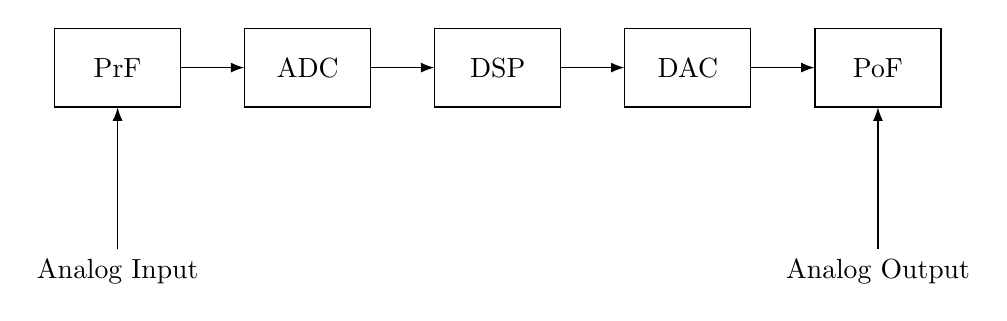
\begin{tikzpicture}[
  node distance=1.8cm and 0.8cm,
  box/.style={draw, minimum width=1.6cm, minimum height=1cm},
  arrow/.style={-Latex}
]
    

% Nodes
\node[box] (n1) {PrF};
\node[box, right=of n1] (n2) {ADC};
\node[box, right=of n2] (n3) {DSP};
\node[box, right=of n3] (n4) {DAC};
\node[box, right=of n4] (null) {PoF};
\node[below=of n1] (n5) {Analog Input};
\node[below=of null] (n6) {Analog Output};

% Pointers
\draw[arrow] (n5) -- (n1);
\draw[arrow] (n1) -- (n2);
\draw[arrow] (n2) -- (n3);
\draw[arrow] (n3) -- (n4);
\draw[arrow] (n4) -- (null);
\draw[arrow] (n6) -- (null);
\end{tikzpicture}

\vspace{1em}
Keywords: \\
PrF - This is a prefilter or an antialiasing filter, which conditions the analog
signal to prevent aliasing. \\
ADC: This is an analog-to-digital converter, which produces a stream of
binary numbers from analog signals. \\
Digital Signal Processor: This is the heart of DSP and can represent a general purpose computer or a special-purpose processor, or digital hardware,
and so on. \\
DAC: This is the inverse operation to the ADC, called a digital-to-analog
converter, which produces a staircase waveform from a sequence of
binary numbers, a first step toward producing an analog signal. \\
PoF: This is a postfilter to smooth out staircase waveform into the desired
analog signal. \\

\newpage
\subsection{Advantages of DSP}

\begin{itemize}
    \item  Systems using the DSP approach can be developed using software running on a general-purpose computer. Therefore DSP is relatively convenient to develop and test, and the software is portable.
    \item DSP operations are based solely on additions and multiplications, leading to extremely stable processing capability, for example, stability independent of temperature.
    \item DSP operations can easily be modified in real time, often by simple
    programming changes, or by reloading of registers.
    \item The DSP has a lower cost because of VLSI technology, which reduces the costs of memories, gates, microprocessors, etc.
\end{itemize}
\subsection{Key Disadvantage}
The principal disadvantage of DSP is the limited speed of operations
limited by the DSP hardware, especially at very high frequencies. Primarily because of its advantages, DSP is now becoming a first choice in many
technologies and applications, such as consumer electronics, communications, wireless telephones, and medical imaging.

\subsection{Advantages over Analog Signal Processing}
\begin{itemize}
    \item Quick reconfiguration. A digital programmable system allows flexibility in reconfiguring the
digital signal processing operations simply by changing the program
    \item Accuracy. Tolerances in analog circuit components make it extremely
difficult for the system designer to control the accuracy of an analog signal processing system. 
    \item Some components may not be available in the construction of the analog circuitry, so DSP may be preferred. 
    \item Cheaper. DSP is cheaper than purchasing parts. 
\end{itemize}


\subsection{Types of DSP}
Most DSP operations can be categorized as being either signal analysis
tasks or signal filtering tasks:

\subsubsection{Signal Analysis}
\begin{itemize}
    \item spectrum (frequency and/or phase) analysis
    \item speech recognition
    \item speaker verification
    \item target detection
\end{itemize}

\subsubsection{Signal filtering}
This task is characterized by the signal-in signal-out
situation. The systems that perform this task are generally called filters.
It is usually (but not always) a time-domain operation. Some of the applications are

\begin{itemize}
    \item removal of unwanted background noise
    \item removal of interference
    \item separation of frequency bands
    \item shaping of the signal spectrum
    
\end{itemize}
In some applications, such as voice synthesis, a signal is first analyzed
to study its characteristics, which are then used in digital filtering to
generate a synthetic voice.

\subsection{Applications of DSP}
\begin{itemize}
    \item speech/audio (speech recognition/synthesis, digital audio, equalization, etc.)
    \item image/video (enhancement, coding for storage and transmission,
    robotic vision, animation, etc.)
    \item military/space (radar processing, secure communication, missile guidance, sonar processing, etc.)
    \item biomedical/health care (scanners, ECG analysis, X-ray analysis, EEG
    brain mappers, etc.)
\end{itemize}
\begin{tabularx}{\textwidth}{|X|X|X|}

\end{tabularx}

\subsection{DSP Hardware (unfinished)}
There are many different hardware options for DSP. It is possible to implement DSP algorithms on any digital computer, but different applications and algorithms shape the type of hardware that is used. There are five main hardware platforms used for DSP:
\begin{itemize}
    \item Special-purpose chips / application specific integrated circuits (ASIC)
    \item Field-Programmable Gate Array (FPGA) 
    \item General-Purpose Microprocessors or Microcontrollers 
    \item General-Purpose DSP processors 
    \item DSP processors with application specific hardware accelerators
\end{itemize}

\section{Basic DSP Scripts in MATLAB}
\subsection{Basic signals}
Consider the signal: \\
\[
x(t) = sin(2\pi t ) + \frac{1}{3}sin(5\pi t )+\frac{1}{5}sin(10\pi t )=\sum_{k=1}^{3}\frac{1}{k}sin(2\pi kt), 0 \leq t \leq 1
\]

Using MATLAB, we want to generate samples of x(t) at time instances
0:0.01:1. We will discuss two approaches.

\subsubsection{Approach 1}
Here we will consider a typical C or Fortran approach, that is, we will use two
for..end loops, one each on t and k. This is the most inefficient approach in
MATLAB, but possible
\begin{lstlisting}
 t = 0:0.01:1; N = length(t); xt = zeros(1,N);
 for n = 1:N
      temp = 0;
      for k = 1:3
          temp = temp + (1/k)*sin(2*pi*k*t(n));
      end
      xt(n) = temp;
 end
    
\end{lstlisting}
\subsubsection{Approach 2}
In this approach, we will compute each sinusoidal component in one step as a
vector, using the time vector t = 0:0.01:1 and then add all components using
one for..end loop.
\begin{lstlisting}
 t = 0:0.01:1; xt = zeros(1,length(t));
 for k = 1:3
 xt = xt + (1/k)*sin(2*pi*k*t);
 end
\end{lstlisting}

\subsection{Fourier signals}
Consider the signal: \\
\[
x(t) = \sum_{k=1}^{K}c_{k}sin(2\pi kt )
\]
If we want to experiment with different values of the coefficients ck and/or
the number of terms K, then we should create a script file.
\begin{lstlisting}[language=MATLAB]
t = 0:0.01:1; k = 1:2:5; ck = 1./k;
xt = ck * sin(2*pi*k'*t);    
\end{lstlisting}

\subsection{Functions}
Source code for the above program written as a function: \\
\begin{lstlisting}[language=MATLAB]
function xt = sinsum(t,ck)
% Computes sum of sinusoidal terms of the form in (1.1)
%x= sinsum(t,ck)
%
K = length(ck); k = 1:K;
ck = ck(:)'; t = t(:)';
xt = ck * sin(2*pi*k'*t);    
\end{lstlisting}
The vectors t and ck should be assigned prior to using the sinsum
function. Note that ck(:)' and t(:)' use indexing and transposition
operations to force them to be row vectors. 

\subsection{Plotting}
One of the most powerful features of MATLAB for signal and data analysis
is its graphical data plotting. MATLAB provides several types of plot,
starting with simple two-dimensional (2D) graphs to complex, higher-dimensional plots with full-color capability. 

We will examine only the 2D 
plotting, which is the plotting of one vector versus another in a 2D coordinate system. The basic plotting command is the plot(t,x) command,
which generates a plot of x values versus t values in a separate figure
window.

\subsubsection{Simple CT Sine wave}
The following set of commands creates a list of sample points, evaluates the sine function at those points, and then generates a plot of a
simple sinusoidal wave, putting axis labels and title on the plot.
\begin{lstlisting}[language=MATLAB]
 t = 0:0.01:2; % sample points from 0 to 2 in steps of 0.01
 x = sin(2*pi*t); % Evaluate sin(2 pi t)
 plot(t,x,'b'); % Create plot with blue line
 xlabel('t in sec'); ylabel('x(t)'); % Label axis
 title('Plot of sin(2\pi t)'); % Title plot    
\end{lstlisting}
\subsubsection{Simple DT Sine Wave}
For plotting a set of discrete numbers (or discrete-time signals), we
will use the stem command which displays data values as a stem, that
is, a small circle at the end of a line connecting it to the horizontal axis.
The circle can be open (default) or filled (using the option 'filled').
Using Handle Graphics (MATLAB's extensive manipulation of graphics
primitives).
\begin{lstlisting}
 n = 0:1:40; % sample index from 0 to 20
 x = sin(0.1*pi*n); % Evaluate sin(0.2 pi n)
 Hs = stem(n,x,'b','filled'); % Stem-plot with handle Hs
 set(Hs,'markersize',4); % Change circle size
 xlabel('n'); ylabel('x(n)'); % Label axis
 title('Stem Plot of sin(0.2 pi n)'); % Title plot    
\end{lstlisting}
\subsubsection{Dirac Signal DT}
The Unit Step signal is defined as: \\
\begin{equation}
\delta(n) = \begin{cases}
1 , &  n = 0 \\
0, & n\neq 0
\end{cases}
\end{equation}
In MATLAB the function zeros(1,N) generates a row vector of N
zeros, which can be used to implement $\delta$(n) over a finite interval. However, the logical relation n==0 is an elegant way of implementing $\delta$(n).
For example, to implement
\begin{equation}
\delta(n-n_o) = \begin{cases}
1 , &  n = n_o \\
0, & n\neq n_o
\end{cases}
\end{equation}
We use the following MATLAB function \\
\begin{lstlisting}
function [x,n] = impseq(n0,n1,n2)
% This defines a function named 'impseq' 
% Takes three inputs: `n0`, `n1`, and `n2`
% - Returns two outputs: 
% 'x':  the step sequence values  
%  'n': the corresponding time indices
% Generates x(n) = delta(n-n0); n1 <= n <= n2
% ----------------------------------------------
% [x,n] = impseq(n0,n1,n2)
%
n = [n1:n2]; x = [(n-n0) == 0];    
\end{lstlisting}

\subsubsection{Unit Step Signal DT}
\begin{lstlisting}
function [x,n] = stepseq(n0,n1,n2)
% Generates x(n) = u(n-n0); n1 <= n <= n2
% ------------------------------------------
% [x,n] = stepseq(n0,n1,n2)
%
n = [n1:n2]; x = [(n-n0) >= 0];
\end{lstlisting}

\subsubsection{Real Exponential Signal}
\begin{equation}
x(n) = a^n, \forall n; a\in\Re
\end{equation}
\begin{lstlisting}
 n = [0:10]; x = (0.9).^n;
\end{lstlisting}
\subsubsection{Complex-value exponential sequence}
\begin{equation}
x(n) = e^{(\sigma+jw_0)n}, \forall n
\end{equation}
\begin{lstlisting}
 n = [0:10]; x = exp((2+3j)*n);
\end{lstlisting}
\subsubsection{Sinusoidal sequence}
\begin{equation}
x(n) = Acos(w_0n+\theta_0),\forall n
\end{equation}
\begin{lstlisting}
 % x(n)=3 cos(0.1*pi*n + pi/3) + 2 sin(0.5*pi*n)
 n = [0:10]; x = 3*cos(0.1*pi*n+pi/3) + 2*sin(0.5*pi*n);    
\end{lstlisting}
\subsubsection{Periodic Signal}
Defined by: \begin{equation}
x(n) = x(n+N) , \forall n
\end{equation}
\begin{lstlisting}
 xtilde = x' * ones(1,P); % P columns of x; x is a row vector
 xtilde = xtilde(:); % long column vector
 xtilde = xtilde'; % long row vector
\end{lstlisting}
\subsection{Source code for some signals}
\begin{equation}
x(n) = 2\delta(n+2)-\delta(n-4), -5\leq n \leq 5.
\end{equation}
\begin{lstlisting}
 n = [-5:5];
 x = 2*impseq(-2,-5,5) - impseq(4,-5,5);
 stem(n,x); title('Sequence in Problem 2.1a')
 xlabel('n'); ylabel('x(n)');    
\end{lstlisting}
\begin{equation}
x(n) = n[u(n)-u(n-10)]+10e^{-0.3(n-10)}[u(n-10)-u(n-20)], 0 \leq n \leq 20
\end{equation}
\begin{lstlisting}
 n = [0:20]; x1 = n.*(stepseq(0,0,20)-stepseq(10,0,20));
 x2 = 10*exp(-0.3*(n-10)).*(stepseq(10,0,20)-stepseq(20,0,20));
 x = x1+x2;
 subplot(2,2,3); stem(n,x); title('Sequence in Problem 2.1b')
 xlabel('n'); ylabel('x(n)');
\end{lstlisting}
\begin{equation}
x(n) = {..., 5, 4, 3, 2, 1, 5, 4, 3, 2, 1, 5, 4, 3, 2, 1, ...}; -10 \leq n \leq 9.
\end{equation}
\begin{lstlisting}[language=MATLAB]
 n = [-10:9]; x = [5,4,3,2,1];
 xtilde = x' * ones(1,4); xtilde = (xtilde(:))';
 subplot(2,2,4); stem(n,xtilde); title('Sequence in Problem 2.1d')
 xlabel('n'); ylabel('xtilde(n)');
\end{lstlisting}

\subsection{Operations on signals}
\subsubsection{Shifting}
In this operation, each sample of x(n) is shifted by an
amount k to obtain a shifted sequence y(n).
\begin{equation}
y(n) = {x(n-k)}
\end{equation}
\begin{lstlisting}
function [y,n] = sigshift(x,m,k)
% implements y(n) = x(n-k)
% -------------------------
% [y,n] = sigshift(x,m,k)
%
n = m+k; y = x;
\end{lstlisting}
\subsubsection{Folding}
In this operation each sample of x(n) is flipped around n = 0
to obtain a folded sequence y(n).
\begin{equation}
y(n) = {x(-n)}
\end{equation}
\begin{lstlisting}
function [y,n] = sigfold(x,n)
% implements y(n) = x(-n)
% -----------------------
% [y,n] = sigfold(x,n)
%
y = fliplr(x); n = -fliplr(n);    
\end{lstlisting}
\subsubsection{Convolution}
\begin{equation}
y(n) = x(n)*h(n)
\end{equation}
Given the sequences \\
x(n) = [3, 11, 7, 0, -1, 4, 2]; $-3 \leq n \leq 3$;

h(n) = [2, 3, 0, -5, 2, 1], $-1 \leq n \leq 4$;

\begin{lstlisting}
 x = [3, 11, 7, 0, -1, 4, 2]; h = [2, 3, 0, -5, 2, 1];
 y = conv(x, h)
%output
y =
6 31 47 6 -51 -5 41 18 -22 -3 8 2    
\end{lstlisting}
The default convolution function works when no timing information is required, but if there is timing information required, other methods must be used. The below function is a modified version of the convolution function.
\begin{lstlisting}
function [y,ny] = conv_m(x,nx,h,nh)
% Modified convolution routine for signal processing
% --------------------------------------------------
% [y,ny] = conv_m(x,nx,h,nh)
% [y,ny] = convolution result
% [x,nx] = first signal
% [h,nh] = second signal
%
nyb = nx(1)+nh(1); nye = nx(length(x)) + nh(length(h));
ny = [nyb:nye]; y = conv(x,h);    
\end{lstlisting}
Solution to above program with new function:
\begin{lstlisting}
 x = [3, 11, 7, 0, -1, 4, 2]; nx = [-3:3];
 h = [2, 3, 0, -5, 2, 1]; ny = [-1:4];
 [y,ny] = conv_m(x,nx,h,nh)
%output 
y =
6 31 47 6 -51 -5 41 18 -22 -3 8 2
ny =
-4 -3 -2 -1 0 1 2 3 4 5 6 7
\end{lstlisting}

\subsection{Digital Filters}
Filter is a generic name that means a linear time-invariant system designed
for a specific job of frequency selection or frequency discrimination. Hence
discrete-time LTI systems are also called digital filters. There are two
types of digital filters.
\subsubsection{FIR filter}
If the unit impulse response of an LTI system is of finite
duration, then the system is called a finite-duration impulse response (or
FIR) filter. Hence for an FIR filter h(n) = 0 for n<n1 and for n>n2.
The following part of the difference equation (2.21) describes a causal FIR
filter:
\begin{equation}
y(n) = \sum_{m=0}^{M}b_mx(n-m)
\end{equation}
\subsubsection{IIR filter}
If the impulse response of an LTI system is of infinite duration, then the system is called an infinite-duration impulse response (or
IIR) filter. The following part of the difference equation describes a recursive filter in which the output y(n) is recursively computed from its previously computed values and is called an autoregressive
(AR) filter. The impulse response of such filter is of infinite duration and
hence it represents an IIR filter. The general equation (2.21) also describes
an IIR filter. It has two parts: an AR part and an MA part. Such an IIR
filter is called an autoregressive moving average, or an ARMA, filter. In
MATLAB, IIR filters are described by the difference equation coefficients
{bm} and {ak} and are implemented by the filter(b,a,x) function.

\begin{equation}
 x(n) = \sum_{k=0}^{K}a_ky(n-k)   
\end{equation}

\newpage
\section{ADC \& DAC}
\subsection{Terminology}
\begin{itemize}
    \item Sampling. This is the conversion of a continuous-time signal into a discrete-time signal obtained by taking “samples” of the continuous-time signal at discrete time instants. Thus, if xa(t) is the input to the sampler, the output is $x_a(nT)$ = x(n), where T is called the sampling interval.
    \item Quantization. This is the conversion of a discrete-time continuous-valued signal into a discrete-time, discrete-valued (digital) signal. The value of each signal sample is represented by a value selected from a finite set of possible values. The difference between the unquantized sample x(n) and the quantized output xq (n) is called the quantization error.
    \item Reconstruction. This is the reconstruction of a digital signal into an analog signal.
\end{itemize}
https://www.geeksforgeeks.org/sample-and-hold-circuit/
\subsection{Sampling of Analog Signals}
Unfiform sampling or periodic sampling can be described by the relation:
\begin{equation}
x(n) = x_a(nT), -\infty<n<\infty
\end{equation}
where x(n) is the discrete time signal obtained by taking samples of the analog signal $x_a(t)$ every \textit{T} seconds. \textit{T} is described as the "sampling period" or the "sampling interval". The recriprocal: $\frac{1}{T}=F_s$ is called the "sampling rate" or the "sampling frequency". \textit{F} can be denoted as the frequency variable for analog signals and \textit{f} can be denoted as the frequency var for discrete signals. \textit{t} and \textit{n} are time vars for continuous and discrete time respectively. The relationship between the variables can be defined by the equation:
\begin{equation}
t = nT = \frac{n}{F_s}
\end{equation}

\begin{figure}[H]
    \centering
    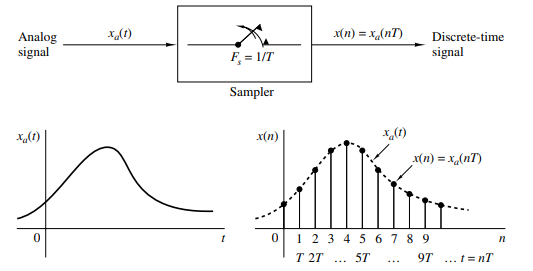
\includegraphics[width=0.8\linewidth]{Periodic_Analog_Signal.png}
    \caption{Periodic sampling of an analog signal}
    \label{fig:enter-label}
\end{figure}

$x_a(t)$, the analog signal in the above figure can be represented as:
\begin{equation}
x_a(t) = A\cos(2\pi Ft + \theta)
\end{equation}
when sampled periodically at a rate $F_s= \frac{1}{T}$ samples per second, yields 
\begin{equation}
x_a(nT) = x(n) = A\cos(2\pi FnT + \theta) = A\cos(\frac{2\pi nF}{F_s}+ \theta)
\end{equation}
Similarly, the relationship between \textit{F} and \textit{f}
\begin{equation}
f = \frac{F}{F_s}
\end{equation}
This relation works if Fs is known. In addition to this, for CT the range of frequency is:
\begin{equation}
-\infty < F < \infty
\end{equation}
but in DT the range is:
\begin{equation}
-\frac{1}{2} < f < \frac{1}{2}  = -\pi < w < \pi 
\end{equation}
because of this $F_s$ must fall in the range 
\begin{equation}
-\frac{1}{2T}=-\frac{F_s}{2}\leq F \leq \frac{F_s}{2} = \frac{1}{2T}
\end{equation}
to prevent aliasing (distortion)

\subsubsection{Sampling examples}
Consider the CT signals: 
\begin{center}
$x_1(t) = \cos2\pi(10)t$ \\
\vspace{1em}
$x_2(t) = \cos2\pi(50)t$
\end{center}
When sampled at $Fs = 40$ Hz. The corresponding DT signals are:
\begin{center}
$x_1(n) = \cos2\pi(\frac{10}{40})n  = \cos(\frac{\pi}{2})n$ \\
\vspace{1em}
$x_2(t) = \cos2\pi(\frac{50}{40})n = \cos(\frac{5\pi}{2})n$
\end{center}
However $\cos(\frac{5\pi}{2})n$ = $\cos(2\pi n + \frac{\pi n}{2})=  \cos( \frac{\pi n}{2})$ meaning the signals are identical. Since 50Hz is greater than half the sampling frequency, this essentially means that the 50Hz signal is an alias of the 10Hz signal.
\vspace{1em}
given the signal:
\begin{center}
$x_a(t) = 3\cos(100\pi t)$ \\
\vspace{1em}
The minimum sampling rate is 2F which is $50*2 = 100$Hz = $F_s$
\vspace{1em}
The discrete time signal after sampling at 100Hz: $A\cos(\frac{2\pi nF}{F_s}+ \theta) =$ $3\cos(\frac{100\pi}{100})n$
\end{center}
Consider the analog signal defined by 
\begin{center}
$x_a(t) = e^{-1000|t|}$
\end{center}
Determine and plot its Fourier transform. \\

\vspace{1em}
The Fourier transform formula of an analog signal in MATLAB is:
\begin{center}
$X_a(jw) = \Delta t \sum_m x_G(m)e^{-jwm\Delta t}$
\end{center}
Where $\Delta t $ is the grid interval and $x_G(m)$ is a finite grid sequence.
Skipping the mathematical explanation, we find that the Fourier transform is 
\begin{center}
$$X_a(jw)= \frac{0.002}{1+(\frac{w}{1000})^2}$$
\end{center}
since $e^{-5} \simeq 0$ (roughly), we can discern that $\Delta t =5*10^{-5}$.
This is because in order to obtain $e^{-5}$ from $e^{-1000|t|}$ , $ t$ must equal $5*10^{-5}$. \\
\vspace{1em}
Similarly, $X_a(jw) = 0$ for $w \geq 2\pi(2000)$. This satisfies the Nquist criterion: $f_{max} \leq \frac{1}{2 \Delta t}  \rightarrow \Delta t \leq \frac{1}{2f_{max}}=\frac{1}{2(2000)}$
\begin{lstlisting}
% Analog Signal
 Dt = 0.00005; t = -0.005:Dt:0.005; xa = exp(-1000*abs(t));
% Continuous-time Fourier Transform
Wmax = 2*pi*2000; K = 500; k = 0:1:K; W = k*Wmax/K;
Xa = xa * exp(-j*t'*W) * Dt; Xa = real(Xa);
W = [-fliplr(W), W(2:501)]; % Omega from -Wmax to Wmax
Xa = [fliplr(Xa), Xa(2:501)]; % Xa over -Wmax to Wmax interval
subplot(2,1,1);plot(t*1000,xa);
xlabel('t in msec.'); ylabel('xa(t)')
title('Analog Signal')
subplot(2,1,2);plot(W/(2*pi*1000),Xa*1000);
xlabel('Frequency in KHz'); ylabel('Xa(jW)*1000')
title('Continuous-time Fourier Transform')    
\end{lstlisting}
Figure 3.11 shows the plots of $x_a(t)$ and $X_a(j\Omega)$. Note that to reduce the number
of computations, we computed $X_a(j\Omega)$ over $[0, 4000\pi]$ rad/sec (or equivalently,
over [0, 2] KHz) and then duplicated it over [$-4000\pi$, 0] for plotting purposes.
The displayed plot of $X_a(j\Omega)$ agrees with (3.36). \\
\vspace{1em}
To study the effect of sampling on the frequency-domain quantities, we will
sample $x_a(t)$ in Example 3.18 at two different sampling frequencies. \\
\vspace{1em}
a. Sample $x_a(t)$ at Fs = 5000 sam/sec to obtain $x_1(n)$. Determine and plot $X_1(e^{j\omega})$. \\
b. Sample $x_a(t)$ at Fs = 1000 sam/sec to obtain $x_2(n)$. Determine and plot $X_2(e^{j\omega})$. \\ 
\vspace{1em}
a. Since the bandwidth of xa(t) is 2KHz, the Nyquist rate is 4000 sam/sec,
which is less than the given Fs. Therefore, aliasing will be (almost) nonexistent.
\begin{lstlisting}
% Analog signal
 Dt = 0.00005; t = -0.005:Dt:0.005; xa = exp(-1000*abs(t));
% Discrete-time signal
 Ts = 0.0002; n = -25:1:25; x = exp(-1000*abs(n*Ts));
% Discrete-time Fourier transform
 K = 500; k = 0:1:K; w = pi*k/K;
 X = x * exp(-j*n'*w); X = real(X);
 w = [-fliplr(w), w(2:K+1)]; X = [fliplr(X), X(2:K+1)];
 subplot(2,1,1);plot(t*1000,xa);
 xlabel('t in msec'); ylabel('Amplitude')
 title('Discrete Signal'); hold on
 stem(n*Ts*1000,x); gtext('Ts=0.2 msec'); hold off
 subplot(2,1,2);plot(w/pi,X);
 xlabel('Frequency in \pi Units'); ylabel('Amplitude')
 title('Discrete-Time Fourier Transform')
\end{lstlisting}
\begin{figure}[H]
    \centering
    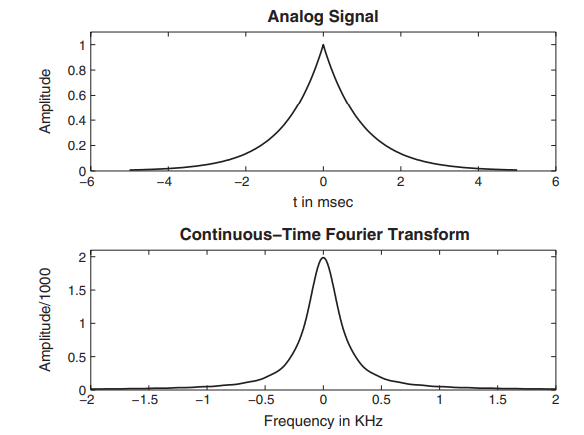
\includegraphics[width=1\linewidth]{SampleFreq.png}
\end{figure}
\begin{figure}[H]
    \centering
    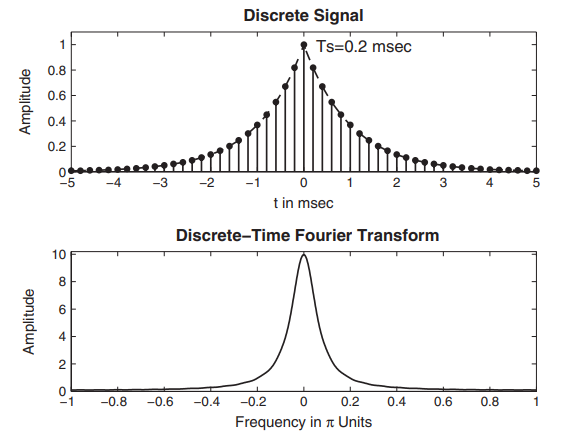
\includegraphics[width=1\linewidth]{DTFreqSamp.png}
\end{figure}
b. Here Fs = 1000 $<$ 4000. Hence there will be a considerable amount of aliasing. This is evident from Figure 3.13, in which the shape of $X(e^{jw})$ is different
from that of $X_a(j\Omega)$ and can be seen to be a result of adding overlapping
replicas of $X_a(j\Omega)$. \\
\begin{figure}[H]
    \centering
    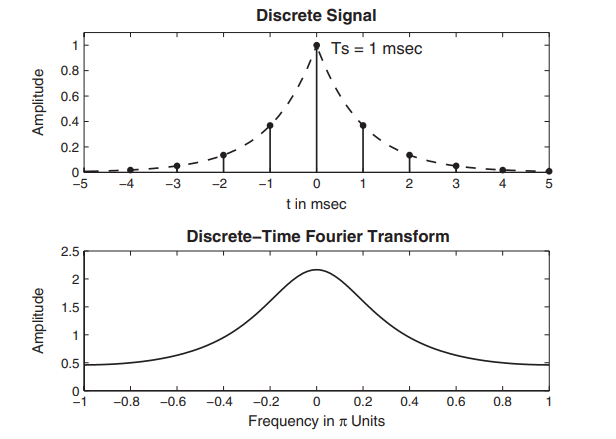
\includegraphics[width=1\linewidth]{AliasedFreq.png}
\end{figure}
\subsection{Summary of ADC}
\begin{tabular}{|c|c|}
\hline
\textbf{Term} & \textbf{Meaning}  \\
\hline
t & CT time \\
\hline
n & DT samples \\
\hline
F & CT frequency \\
\hline
f & DT frequency \\
\hline
$t = nT = \frac{n}{Fs}$ & Relation between CT and DT time\\
$A\cos(\frac{2\pi nF}{F_s}+ \theta) $ & DT sinusoid representation \\
\hline
$F_s \geq 2F$ & Minimum sampling rate to prevent aliasing \\

\hline
\end{tabular}
\subsection{Reconstruction (D/A)}
From the sampling theorem and the preceding examples, it is clear that if
we sample band-limited xa(t) above its Nyquist rate, then we can reconstruct xa(t) from its samples x(n). This reconstruction can be thought of
as a two-step process: \\
First, the samples are converted into a weighted impulse train:
$$\sum_{n=-\infty}^{\infty}x(n)\delta(t-nT_s) = ...+x(-1)\delta(n+T_s)+x(0)\delta(t)+x(1)\delta(n-T_s)+...$$
Then, the impulse train is filtered through an ideal analog lowpass filter
band-limited to the [-Fs/2, Fs/2] band \\
\vspace{1em}
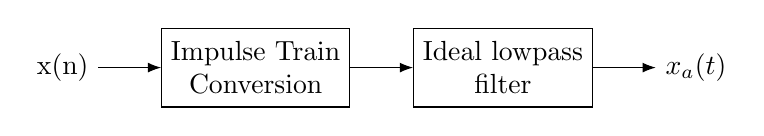
\begin{tikzpicture}[
  node distance=1.8cm and 0.8cm,
  box/.style={draw, minimum width=1.6cm, minimum height=1cm,align=center},
  arrow/.style={-Latex}
]
    

% Nodes
\node[] (n1) {x(n)};
\node[box, right=of n1] (n2) {Impulse Train \\ Conversion};
\node[box, right=of n2] (n3) {Ideal lowpass \\ filter};
\node[right=of n3] (n4) {$x_a(t)$};

% Pointers
\draw[arrow] (n1) -- (n2);
\draw[arrow] (n2) -- (n3);
\draw[arrow] (n3) -- (n4);
\end{tikzpicture} \\
This two-step procedure can be described mathematically using an interpolating formula 
\begin{equation}
x_a(t)=\sum_{n=-\infty}^{\infty}x(n)sinc[F_s(t-nT_s)]
\end{equation}
where sinc(x) = $\frac{\sin\pi x}{\pi x}$ is an interpolating function. The physical interpretation of the above reconstruction (3.37) is given in Figure 3.14, from
which we observe that this ideal interpolation is not practically feasible,
because the entire system is noncausal and hence not realizable. 
\begin{figure}[H]
    \centering
    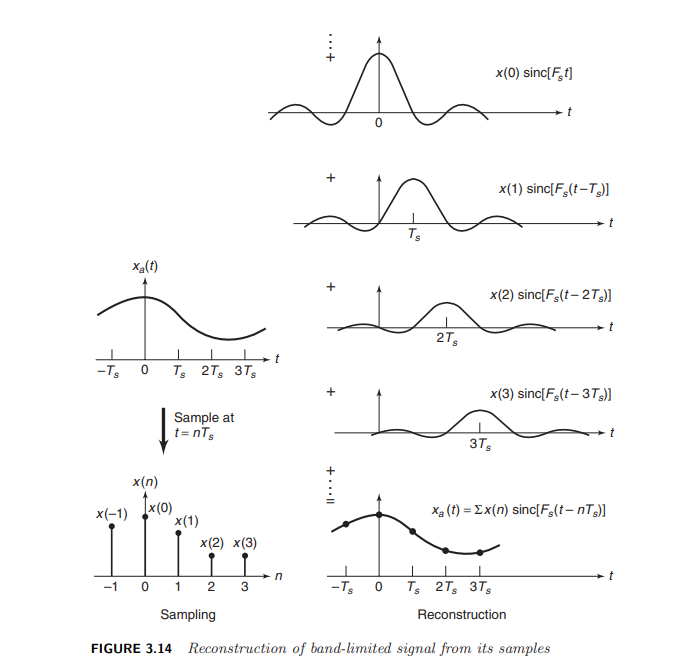
\includegraphics[width=0.8\linewidth]{ReconstructionVisual.png}
\end{figure}
\subsubsection{Reconstruction examples}
Consider the sampled signal x(n) from Example 3.17: $x_a(t) = 4 +2\cos(150\pi t + \pi/3) + 4\sin(350\pi t)$. It is applied as an
input to an ideal D/A converter (i.e., an ideal interpolator) to obtain the
analog signal $y_a(t)$. The ideal D/A converter is also operating at $F_s$ = 200
sam/sec. Obtain the reconstructed signal $y_a(t)$, and determine whether the
sampling/reconstruction operation resulted in any aliasing. Also, plot the
Fourier transforms $X_a(j\Omega)$, $X(e^{jw})$, and $Y_a(j\Omega)$. \\
\vspace{1em}
We can determine $y_a(t)$ using (3.31). However, since all frequencies in the sinusoidal sequence x(n) are between the primary period of $-\pi \leq \omega \leq \pi$, we can
equivalently obtain $y_a(t)$ by substituting n by $tF_s$. \\
\vspace{1em}
$y_a(t) = x(n) |_{n=tFs}=x(n)|_{n=200t}=4+2\cos(0.75\pi200t+\frac{\pi}{3})-4\sin(0.25\pi200t)$ 

\begin{figure}[H]
    \centering
    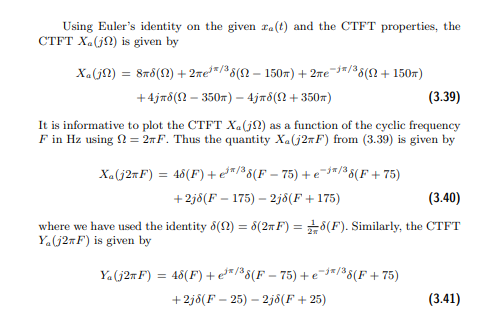
\includegraphics[width=1\linewidth]{DAexample1.png}

\end{figure}
\begin{figure}[H]
    \centering
    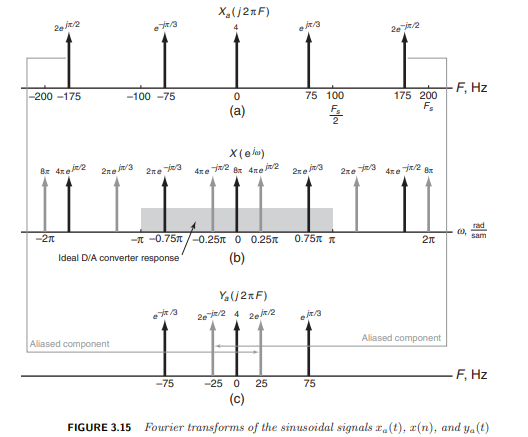
\includegraphics[width=1\linewidth]{FourierDAexample1.png}
\end{figure}

\subsubsection{Practical D/A converters}
In practice, we need a different approach
than the interpolating formula. The two-step procedure is still feasible, but now we replace
the ideal lowpass filter by a practical analog lowpass filter. Another interpretation of (23) is that it is an infinite-order interpolation. We want
finite-order (and in fact low-order) interpolations. There are several approaches to do this. \\
\vspace{1em}
\textbf{Zero-order-hold (ZOH)} interpolation: In this interpolation, a
given sample value is held for the sample interval until the next sample
is received,
\begin{center}
$\hat{x}_a(t)  = x(n), \space nT_s \leq n \leq (n+1)T_s$
\end{center}
which can be obtained by filtering the impulse train through an interpolating filter of the form. $\hat{x}_a(t)$ is the analog signal before filtering is applied. 
\begin{center}
    $h_0(t)= \begin{cases}
        1, & 0 \leq t \leq T_s \\
        0, & \text{otherwise}
    \end{cases}$
\end{center}
which is a rectangular pulse. The resulting signal is a piecewise-constant
(staircase) waveform that requires an appropriately designed analog
postfilter for accurate waveform reconstruction. \\
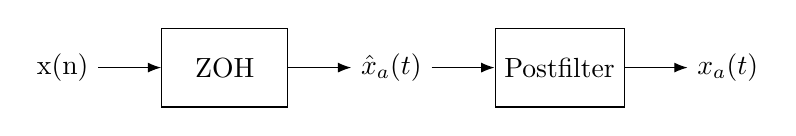
\begin{tikzpicture}[
  node distance=1.8cm and 0.8cm,
  box/.style={draw, minimum width=1.6cm, minimum height=1cm,align=center},
  arrow/.style={-Latex}
]
    

% Nodes
\node[] (n1) {x(n)};
\node[box, right=of n1] (n2) {ZOH};
\node[right=of n2] (n3) {$\hat{x}_a(t)$};
\node[box, right=of n3] (n4) {Postfilter};
\node[right=of n4] (n5) {$x_a(t)$};
% Pointers
\draw[arrow] (n1) -- (n2);
\draw[arrow] (n2) -- (n3);
\draw[arrow] (n3) -- (n4);
\draw[arrow] (n4) -- (n5);
\end{tikzpicture} \\
\vspace{1em}
\textbf{First-order-hold (FOH) interpolation}: In this case, the adjacent
samples are joined by straight lines. This can be obtained by filtering
the impulse train through \\
\vspace{1em}
\begin{equation}
h_1(t) = \begin{cases}
1 + \frac{t}{T_s}, & 0 \leq t \leq T_s \\
1 - \frac{t}{T_s}, & T_s \leq t \leq 2T_s \\
0, & \text{otherwise}
\end{cases}
\end{equation}
Once again, an appropriately designed analog postfilter is required for
accurate reconstruction. These interpolations can be extended to higher orders. One particularly useful interpolation employed by MATLAB is
the following. \\
\vspace{1em}
\textbf{Cubic spline interpolation}: This approach uses spline interpolants
for a smoother, but not necessarily more accurate, estimate of the analog signals between samples. Hence this interpolation does not require
an analog postfilter. The smoother reconstruction is obtained by using a set of piecewise continuous third-order polynomials called cubic
splines, given by \\
\begin{equation}
x_a(t) = \alpha_0(n)+ \alpha_1(n)(t-nT_s)+\alpha_2(n)(t-nT_s)^2+\alpha_3(n)(t-nT_s)^3, \space \space nT_s \leq n < (n+1)T_s
\end{equation}
where ${\alpha_i(n), 0 \leq i \leq 3}$ are the polynomial coefficients, which are determined by using least-squares analysis on the sample values [10].
(Strictly speaking, this is not a causal operation but is a convenient
one in MATLAB.)
\subsubsection{MATLAB implementation}
For interpolation between samples, MATLAB provides several approaches. 
The function sinc(x), which generates the $\sin(\pi x)/\pi x$ function, can
be used to implement interpolation, given a finite number of samples. If \{x(n),$n_1  \leq n \leq n_2$\} is given, and if we want to interpolate $x_a(t)$ on a very fine grid with the grid interval $\Delta t$, then, from the interpolating formula 
\begin{equation}
x_a(m\Delta t) \simeq \sum_{n=n_1}^{n_2}x(n)sinc[F_s(m\Delta t-nT_s)], t_1 \leq m\Delta t\leq t_2
\end{equation}
which can be implemented as a matrix-vector multiplication operation as
shown below.
\begin{lstlisting}
 n = n1:n2; t = t1:t2; Fs = 1/Ts; nTs = n*Ts; % Ts is the sampling interval
 xa = x * sinc(Fs*(ones(length(n),1)*t-nTs'*ones(1,length(t))));
\end{lstlisting}
Note that it is not possible to obtain an exact analog $x_a(t)$ in light of the fact that we have assumed a finite number of samples. We now demonstrate the use of the sinc function in the following two examples and also study the aliasing problem in the time domain. \\
\vspace{1em}
From the samples $x_1(n)$ in Example 3.19a, reconstruct $x_a(t)$ and comment on
the results. \\
\vspace{1em}
Solution: Note that $x_1(n)$ was obtained by sampling $x_a(t)$ at $T_s$ = 1/$F_s$ = 0.0002 sec. We
will use the grid spacing of 0.00005 sec over$ -0.005 \leq t \leq 0.005$, which gives
x(n) over $-25 \leq n \leq 25$.
\begin{lstlisting}
% Discrete-time signal x1(n)
 Ts = 0.0002; n = -25:1:25; nTs = n*Ts; x = exp(-1000*abs(nTs));
% Analog signal reconstruction
 Dt = 0.00005; t = -0.005:Dt:0.005;
 xa = x * sinc(Fs*(ones(length(n),1)*t-nTs'*ones(1,length(t))));
% Check
 error = max(abs(xa - exp(-1000*abs(t))))
error =
0.0363
\end{lstlisting}
\begin{figure}[H]
    \centering
    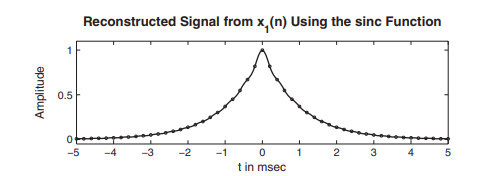
\includegraphics[width=1\linewidth]{SincDAC.png}
\end{figure}
The maximum error between the reconstructed and the actual analog signal is
0.0363, which is due to the fact that xa(t) is not strictly band-limited (and also
we have a finite number of samples). We note that visually
the reconstruction is excellent, however sinc is an ideal DAC and not a real one. \\
\vspace{1em}
From the samples $x_2$(n) in Example 3.17b, reconstruct $x_a$(t) and comment on
the results. \\
\vspace{1em}
In this case, $x_2$(n) was obtained by sampling $x_a(t)$ at $T_s$ = 1/$F_s$ = 0.001 sec.
We will again use the grid spacing of 0.00005 sec over$ -0.005 \leq t \leq 0.005$, which gives
x(n) over $-25 \leq n \leq 25$.
\begin{lstlisting}
% Discrete-time signal x2(n)
 Ts = 0.001; n = -5:1:5; nTs = n*Ts; x = exp(-1000*abs(nTs));
% Analog signal reconstruction
 Dt = 0.00005; t = -0.005:Dt:0.005;
 xa = x * sinc(Fs*(ones(length(n),1)*t-nTs'*ones(1,length(t))));
% Check
 error = max(abs(xa - exp(-1000*abs(t))))
error =
0.1852
\end{lstlisting}
\begin{figure}[H]
    \centering
    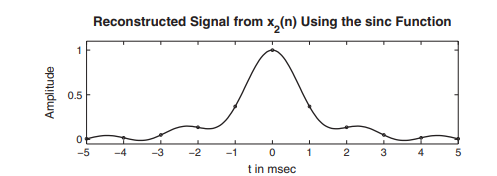
\includegraphics[width=1\linewidth]{SincDAC2.png}
\end{figure}
The maximum error between the reconstructed and the actual analog signals is
0.1852, which is significant and cannot be attributed to the nonband-limitedness
of xa(t) alone. From Figure 3.17, observe that the reconstructed signal differs
from the actual one in many places over the interpolated regions. This is the
visual demonstration of aliasing in the time domain. \\
\vspace{1em}
The second MATLAB approach for signal reconstruction is a plotting
approach. The stairs function plots a staircase (ZOH) rendition of the
analog signal, given its samples, while the plot function depicts a linear
(FOH) interpolation between samples. \\
\vspace{1em}
Plot the reconstructed signal from the samples x1(n) in Example 3.19 using the
ZOH and the FOH interpolations. Comment on the plots.
\begin{lstlisting}
% Discrete-time signal x1(n) : Ts = 0.0002
 Ts = 0.0002; n = -25:1:25; nTs = n*Ts; x = exp(-1000*abs(nTs));
% Plots
 subplot(2,1,1); stairs(nTs*1000,x);
 xlabel('t in msec'); ylabel('Amplitude')
 title('Reconstructed Signal from x_1(n) Using ZOH'); hold on
 stem(n*Ts*1000,x); hold off
%
% Discrete-time signal x1(n) : Ts = 0.001
 Ts = 0.001; n = -5:1:5; nTs = n*Ts; x = exp(-1000*abs(nTs));
% Plots
 subplot(2,1,2); plot(nTs*1000,x);
 xlabel('t in msec'); ylabel('Amplitude')
 title('Reconstructed Signal from x_1(n) Using FOH'); hold on
 stem(n*Ts*1000,x); hold off
\end{lstlisting}
\begin{figure}
    \centering
    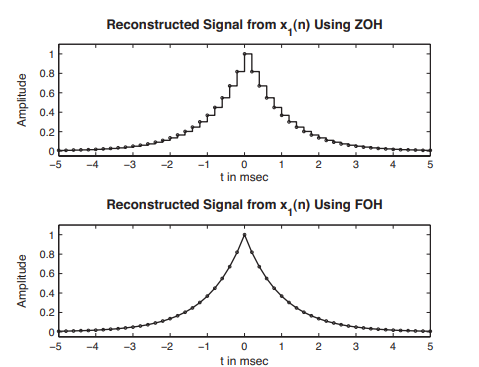
\includegraphics[width=1\linewidth]{ZOHFOH.png}
\end{figure}
The plots are shown in Figure 3.18, from which we observe that the ZOH reconstruction is a crude one and that the further processing of analog signal is
necessary. The FOH reconstruction appears to be a good one, but a careful
observation near t = 0 reveals that the peak of the signal is not correctly reproduced. In general, if the sampling frequency is much higher than the Nyquist
rate, then the FOH interpolation provides an acceptable reconstruction. \\
\vspace{1em}
The third approach of reconstruction in MATLAB involves the use
of cubic spline functions. The spline function implements interpolation
between sample points. It is invoked by xa = spline(nTs,x,t), in which
x and $nT_s$ are arrays containing samples x(n) at $nT_s$ instances, respectively, and t array contains a fine grid at which $x_a(t)$ values are desired.
Note once again that it is not possible to obtain an exact analog $x_a(t)$. \\
From the samples $x_1(n)$ and $x_2(n)$ in Example 3.19, reconstruct $x_a(t)$ using the
spline function. Comment on the results.
\begin{lstlisting}
% a) Discrete-time signal x1(n): Ts = 0.0002
 Ts = 0.0002; n = -25:1:25; nTs = n*Ts; x = exp(-1000*abs(nTs));
% Analog signal reconstruction
 Dt = 0.00005; t = -0.005:Dt:0.005; xa = spline(nTs,x,t);
% Check
 error = max(abs(xa - exp(-1000*abs(t))))
error = 0.0317
% Discrete-time signal x2(n): Ts = 0.001
 Ts = 0.001; n = -5:1:5; nTs = n*Ts; x = exp(-1000*abs(nTs));
% Analog signal reconstruction
 Dt = 0.00005; t = -0.005:Dt:0.005; xa = spline(nTs,x,t);
% Check
 error = max(abs(xa - exp(-1000*abs(t))))
error = 0.1679
\end{lstlisting}
\begin{figure}
    \centering
    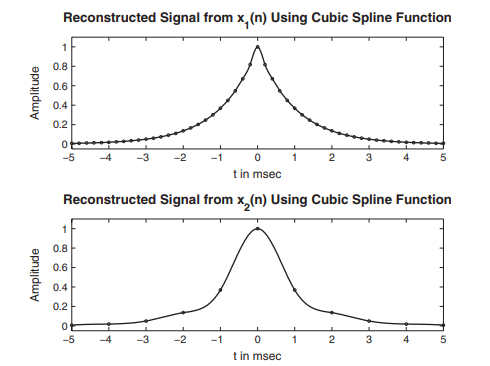
\includegraphics[width=1\linewidth]{Spline.png}
\end{figure}
The maximum error between the reconstructed and the actual analog signal is
0.0317, which is due to the nonideal interpolation and the fact that xa(t) is
nonband-limited. Comparing this error with that from the sinc (or ideal) interpolation, we note that this error is lower. 



\newpage

\section{Discrete Time Fourier Analysis}
The equation of a LTI system can be represented as: \\
\begin{equation}
y(n) = h(n) * x(n)
\end{equation}

\subsection{Definition of the Fourier Transform}
if the magnitude of x(n) is absolutely summable: \\
\begin{equation}
\sum_{-\infty}^{\infty}|x(n)| < \infty
\end{equation}
then the discrete Fourier transform of the signal is given by \\
\begin{equation}
X(e^{jw})= \fourier|x(n)| = \sum_{n=-\infty}^{\infty}x(n)e^{-jwn}
\end{equation}
and then the inverse Fourier tranform is:
\begin{equation}
x(n) = \fourier^{-1}|X(e^{jwn})|=\frac{1}{2\pi}\int_{-\pi}^{\pi}X(e^{jw})e^{jwn}dw
\end{equation}

\subsubsection{examples}
Consider the signal:\\
\begin{equation}
 x(n) = (0.5)^n u(n)    
\end{equation}
Converting to the discrete frequency domain:
\begin{equation}
X(e^{jw})= \fourier|x(n)| = \sum_{n=-\infty}^{\infty}x(n)e^{-jwn} = \sum_{n=0}^{\infty}(0.5)^ne^{-jwn}
\end{equation}
using the geometric series defined by \\
\begin{equation}
\sum_{n=0}^{\infty}ax^n, |x|\leq1 = \frac{a}{1-x}
\end{equation}
We obtain the simplified Fourier transform 
\begin{equation}
= \sum_{n=0}^{\infty}(0.5e^{-jw})^n = \frac{1}{1-0.5e^{-jw}} =  \frac{e^{jw}}{e^{jw}-0.5}
\end{equation}
Final simplification is obtained by multiplying the numerator and denominator by $e^{jwn}$. \\
\vspace{1em}

Given
\begin{equation}
x(n) = {1,2,3,4,5}
\end{equation}

\begin{equation}
X(e^{jw})= \fourier|x(n)| = \sum_{n=-\infty}^{\infty}x(n)e^{-jwn}= e^{jw}+2+3e^{-jw}+4e^{-j2w}+5e^{-j3w}
\end{equation}

\subsection{DTFT in MATLAB}
\subsubsection{DTFT for arbitrary finite signal}
If x(n) is finite and we want to evaluate $X(e^{jw})$ at equispaced frequencies between $[0, \pi]$, then matrix-vector multiplication can be used. Let us assume the sequence x(n) has N samples between $n_1 \leq n \leq n_N$ not necessarily between [0, N-1] and we want to evaluate $X(e^{jw})$ at

\begin{center}
$w_k = \frac{\pi}{M}k$, k = 0,1...,M   
\end{center}
This essentially represents equispaced frequencies between $[0,\pi]$. Then the general frequency response can be written as

\begin{center}
$X(e^{jwk})= \sum_{l=1}^{N}e^{-j(\pi/M)knl}x(n_l), k= 0,1...,M$
\end{center}
This gives:
\begin{lstlisting}
 k = [0:M]; n = [n1:n2];
X=x* (exp(-j*pi/M)) .^ (n'*k);
\end{lstlisting}

The DTFT can easily be performed in MATLAB given an arbitrary signal. \\
Consider the signal: \\
\begin{center}
 $x(n) = (0.9e^{(\frac{j\pi}{3})})^n, 0 \leq n \leq 10$ \\   
\end{center}

We can obtain the plot of the magnitude and phase from $[-2\pi,2\pi]$ in MATLAB
\begin{lstlisting}
 n = 0:10; x = (0.9*exp(j*pi/3)).^n;
 k = -200:200; w = (pi/100)*k; % essentially since k is -200:200 the graph becomes -2pi to 2pi
X=x* (exp(-j*pi/100)) .^ (n'*k);
 magX = abs(X); angX =angle(X);
 subplot(2,1,1); plot(w/pi,magX);grid
 xlabel('frequency in units of pi'); ylabel('|X|')
 title('Magnitude Part')
 subplot(2,1,2); plot(w/pi,angX/pi);grid
 xlabel('frequency in units of pi'); ylabel('radians/pi')
 title('Angle Part')
\end{lstlisting}
Consider the frequency response defined by
\begin{equation}
H(e^{jw})= \frac{1}{1-0.9e^{-jw}}
\end{equation}
\begin{lstlisting}
 w = [0:1:500]*pi/500; % [0, pi] axis divided into 501 points.
 H = exp(j*w) ./ (exp(j*w) - 0.9*ones(1,501));
 magH = abs(H); angH = angle(H);
 subplot(2,1,1); plot(w/pi,magH); grid;
 xlabel('frequency in pi units'); ylabel('|H|');
 title('Magnitude Response');
 subplot(2,1,2); plot(w/pi,angH/pi); grid
 xlabel('frequency in pi units'); ylabel('Phase in pi Radians');
 title('Phase Response');    
\end{lstlisting}
\newpage
Consider the Fourier transform from equation 30: 
\begin{center}
$$X(e^{jw})= \frac{e^{jw}}{e^{jw}-0.5}$$
\end{center}
We can obtain the magnitude, angle, real, and imaginary parts at 501 equispaced points between $[0,\pi]$ in MATLAB.
\begin{lstlisting}
 w = [0:1:500]*pi/500; % [0, pi] axis divided into 501 points.
 X = exp(j*w) ./ (exp(j*w) - 0.5*ones(1,501));
 magX = abs(X); angX = angle(X); realX = real(X); imagX = imag(X);
 subplot(2,2,1); plot(w/pi,magX); grid
 xlabel('frequency in pi units'); title('Magnitude Part'); ylabel('Magnitude')
 subplot(2,2,3); plot(w/pi,angX); grid
 xlabel('frequency in pi units'); title('Angle Part'); ylabel('Radians')
 subplot(2,2,2); plot(w/pi,realX); grid
 xlabel('frequency in pi units'); title('Real Part'); ylabel('Real')
 subplot(2,2,4); plot(w/pi,imagX); grid
 xlabel('frequency in pi units'); title('Imaginary Part'); ylabel('Imaginary')    
\end{lstlisting}
\subsubsection{Frequency Response}
Recall from ECE 3704, the equation for frequency response: 
\begin{equation}
H(e^{jw}) = \frac{Y(e^{jw})}{X(e^{jw})}
\end{equation}
Given a difference equation, we can derive its frequency response. The general form of a difference equation can be represented as:
\begin{equation}
y(n) + \sum_{l=1}^{N}a_ly(n-l)= \sum_{m=0}^{M}b_mx(n-m) 
\end{equation}
where $a_l$ and $b_m$ are nothing but coefficients. From this we can obtain the generalized formula:
\begin{equation}
H(e^{jw}) = \frac{\sum_{m=0}^{M}b_me^{jw(n-m)}}{1+\sum_{l=1}^{N}a_le^{-jwl}}
\end{equation}
Consider the LTI system defined by the difference equation \\
\begin{center}
 y(n) = 0.8y(n-1) + x(n)  \\
 given: x(n) = $\cos(0.05\pi n)u(n)$
\end{center}
putting into standard form:
\begin{center}
y(n) - 0.8y(n-1) = x(n)
\end{center}
From here, we can obtain 
\newpage
\begin{center}
$H(e^{jw})==\frac{1}{1-0.8e^{-jw}}$
\end{center}
The input and output plot sequence in MATLAB
\begin{lstlisting}
 subplot(1,1,1)
 b = 1; a = [1,-0.8];
 n=[0:100];x = cos(0.05*pi*n);
 y = filter(b,a,x);
 subplot(2,1,1); stem(n,x);
 xlabel('n'); ylabel('x(n)'); title('Input sequence')
 subplot(2,1,2); stem(n,y);
 xlabel('n'); ylabel('y(n)'); title('Output sequence')   
\end{lstlisting}
A 3rd-order lowpass filter is described by the difference equation 
\begin{center}
$y(n) = 0.0181x(n)+0.0543x(n - 1)+0.0543x(n - 2)+0.0181x(n - 3)
+1.76y(n - 1) - 1.1829y(n - 2)+0.2781y(n - 3)$
    
\end{center}
Plot the magnitude and the phase response of this filter, and verify that it is a lowpass filter.
\begin{lstlisting}
 b = [0.0181, 0.0543, 0.0543, 0.0181]; % filter coefficient array b
 a = [1.0000, -1.7600, 1.1829, -0.2781]; % filter coefficient array a
 m = 0:length(b)-1; l = 0:length(a)-1; % index arrays m and l
 K = 500; k = 0:1:K; % index array k for frequencies
 w = pi*k/K; % [0, pi] axis divided into 501 points.
 num = b * exp(-j*m'*w); % Numerator calculations
 den = a * exp(-j*l'*w); % Denominator calculations
 H = num ./ den; % Frequency response
 magH = abs(H); angH = angle(H); % mag and phase responses    
 subplot(2,1,1); plot(w/pi,magH); grid; axis([0,1,0,1])
 xlabel('frequency in pi units'); ylabel('|H|');
 title('Magnitude Response');
 subplot(2,1,2); plot(w/pi,angH/pi); grid
 xlabel('frequency in pi units'); ylabel('Phase in pi Radians');
 title('Phase Response');
\end{lstlisting}
\subsection{Block Diagrams}

\begin{figure}[H]
    \centering
    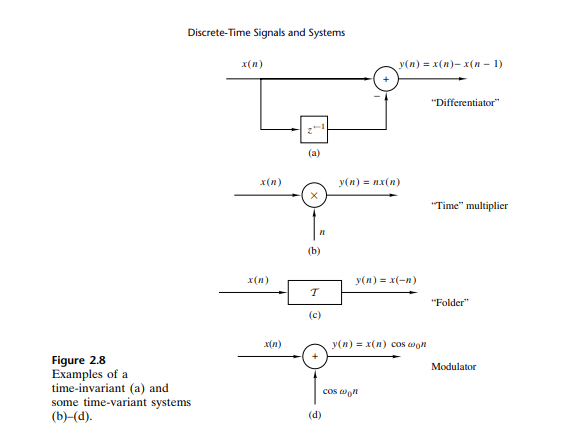
\includegraphics[width=0.7\linewidth]{Blocks.png}
    \label{fig:enter-label}
\end{figure}
\section{Z-transforms (unfinished)}
\subsection{Intro to Z-transforms}
A Fourier Transform of an input sequence x[n] is defined as 
\begin{equation}
X(e^{jw})=\sum_{n=-\infty}^{\infty}x[n]e^{-j\omega n}
\end{equation}
While the Z-transform is defined as 
\begin{equation}
X(z) = \sum_{n=-\infty}^{\infty}x[n]z^{-n}
\end{equation}
Or equivalently
\begin{equation}
Z\{x[n]\}=\sum_{n=-\infty}^{\infty}x[n]z^{-n}=X(z)
\end{equation}
The Z-transform can be thought of as the equivalent of taking the Laplace transform of a signal in discrete time, that is the Z-transform for discrete time signals is a counterpart to the Laplace transform for continuous time signals.
\begin{equation}
X(z) = \sum_{n=0}^{\infty}x[n]z^{-n}
\end{equation}
Is the unilateral z-transform while the bilateral Z-transform is from negative infinity to infinity. The bilateral transform is used when the signal $x[n]$ is non-zero for $n<0$ while unilateral is used when the signal $x[n]$ is zero for $n<0$. An anti-casual signal, that is $x[n] = 0$ for $n \geq 0$ is represented by the equation 
\begin{equation}
X(z) = \sum_{n=-\infty}^{-1}x[n]z^{-n}
\end{equation}

The relationship between the Fourier Transform and Z-transform comes from the equation 
\begin{equation}
z = re^{jw}
\end{equation}
We can further see the relationship in the following equation
\begin{equation}
X(e^{jw}) = \sum_{n=-\infty}^{\infty}x[n](re^{jw})^{-n}
\end{equation}
The Fourier transform corresponds to the Z-transform as long as the Z-transform exists within the unit circle. The main difference between the Z-transform and the Fourier Transform is that the Fourier transform does not converge for all sequences. The convergence of the Z-transform depends only on $|z|$ since $|X(z)| \leq \infty$ if
\begin{equation}
 \sum_{n=-\infty}^{\infty}x[n]|z|^{-n} < \infty
\end{equation}
\subsubsection{Right-Sided Exponential Sequence}
Given the signal $x[n]= a^nu[n]$, find the Z-transform.
\begin{center}
$$X(z) = \sum_{n=-\infty}^{\infty}a^nu[n] =\sum_{n=0}^{\infty}(az^{-1})^n$$
\end{center}
For convergence of X(z), we require that
\begin{center}
$$\sum_{n=0}^{\infty}|az^{-1}|^n < \infty$$
\end{center}
Expanding the Z-transform of x[n] via the power series
\begin{center}
$$\sum_{n=0}^{\infty}(az^{-1})^n = \frac{1}{1-az^{-1}}=\frac{z}{z-a}$$
\end{center}
Therefore $|z| > |a|$ for convergence. This is equivalent to $$\frac{|a|}{|z|}<1$$ which the power series requires $$\sum_{x=0}^{\infty}ax^n,|x|<1$$
\subsubsection{Left-Sided Exponential}
Given the signal $x[n]= -a^nu[n-1]$, find the Z-transform.
\begin{center}
$$X(z) = -\sum_{n=-\infty}^{\infty}a^nu[-n-1]z^{-n} =-\sum_{n=-\infty}^{-1}a^{n}z^{-n}= 1 -\sum_{n=1}^{\infty}(\frac{z}{a}
)^n$$
\end{center}
Expanding the Z-transform of x[n] via the power series
\begin{center}
$$X(z) = -\frac{z/a}{1-z/a}=\frac{z}{a-z}, |a| > |z|$$
\end{center}
From the summation we see that a must be greater than z in order for the magnitude to be less than 1, hence why a must be greater than z for the ROC. The Z-transform table for general signals can be found on the next page.

\begin{tabularx}{\textwidth}{|X|X|X|}
\hline
\textbf{Signal x(n)} & \textbf{z-Transform X(z)} & \textbf{ROC} \\
\hline
$$\delta(n)$$ & $$1$$ & $$\text{All} \space \space \space \space z $$\\
\hline
$$u(n)$$ & $$\frac{1}{1-z^{-1}}$$ & $$|z| > 1 $$  \\
\hline
$$a^nu(n)$$ & $$\frac{1}{1-az^{-1}}$$ & $$|z| > |a|$$   \\
\hline
$$na^nu(n)$$ & $$\frac{az^{-1}}{(1-az^{-1})^2}$$ & $$|z| > |a|$$ \\
\hline
$$-a^nu(-n-1)$$ & $$\frac{1}{1-az^{-1}}$$ & $$|z| < |a|$$ \\
\hline
$$-na^nu(-n-1)$$ & $$\frac{az^{-1}}{(1-az^{-1})^2}$$ & $$|z| < |a|$$  \\
\hline
$$(\cos\omega_0n)u(n)$$ & $$\frac{1-z^{-1}\cos\omega_o}{1-2z^{-1}\cos\omega_o+z^{-2}}$$ & $$|z| > 1$$ \\
\hline
$$(\sin\omega_0n)u(n)$$ & $$\frac{z^{-1}\sin\omega_o}{1-2z^{-1}\cos\omega_o+z^{-2}}$$ & $$|z| > 1$$  \\
\hline
$$(a^n\cos\omega_0n)u(n)$$ & $$\frac{1-az^{-1}\cos\omega_o}{1-2az^{-1}\cos\omega_o+a^2z^{-2}}$$ & $$|z| > |a|$$   \\
\hline
$$(a^n\cos\omega_0n)u(n)$$ & $$\frac{az^{-1}\sin\omega_o}{1-2az^{-1}\cos\omega_o+a^2z^{-2}}$$ & $$|z| > |a|$$ \\
\hline

\end{tabularx} \\    
\subsection{Frequency Response Analysis of Z-transform}
If the poles of H(z) include the unit circle, the frequency response exists. That is, given 
\begin{center}
$$H(z) = \frac{1}{z+0.5}$$
\end{center}
has a frequency response that exists because the pole z = -0.5 is inside the unit circle (magnitude less than 1). 
\subsection{Complex Exponential Response Property}
The frequency response is a complex function that can be expressed in either polar or rectangular form
\begin{equation}
H(e^{jw})=|H(e^{jw})|e^{j<H(e^{jw})}=H_R(e^{jw})+jH_1(e^{jw})
\end{equation}
When the input to a stable LTI system is a complex exponential, the output of the system contains the same frequency with only the phase and frequency manipulated, that is 
\begin{equation}
x[n] = Ae^{j(\omega n+\theta)}\leftrightarrow  A|H(e^{jw})|e^{j(\omega n+\theta+<H(e^{jw}))}
\end{equation}
or
\begin{equation}
x[n] = A\cos(\omega n +\theta) \leftrightarrow A\cos(\omega n + \theta)
\end{equation}
\subsection{Properties of Z-transform (unfinished)}
\begin{tabularx}{\textwidth}{|X|X|}
\hline
\textbf{Property} & \textbf{Transform} \\
\hline
\text{Linearity} & $ a_1 x_1(n) + a_2 x_2(n) \Leftrightarrow a_1 X_1(z) + a_2 X_2(z)$ \\
\hline
\hline
\text{Time Shifting} & $x[n-k] \Leftrightarrow z^{-k}X(z)$ \\
\hline
\hline
\text{Scaling} & $a^nx[n] \Leftrightarrow X(a^{-1}z)$ \\
\hline
\hline
\text{Differentiation} & $$nx[n] \Leftrightarrow -z\frac{dX(z)}{dz}$$ \\
\hline
\hline
\text{Folding} & $x[-n] \Leftrightarrow X(1/z)$ \\
\hline
\hline
\text{Convolution} & $x_1*x_2 \Leftrightarrow X_1X_2$ \\
\hline
\end{tabularx}
\section{Discrete Fourier Transform}
The Discrete Fourier Transform (DFT) is defined by:
\begin{equation}
X(k) =\sum_{n=0}^{N-1}x(n)e^{-j2\pi k n/N}, k =0,1,2....,N-1
\end{equation}
The Inverse Discrete Fourier Transform (IDFT) is defined by:
\begin{equation}
x(n) = \frac{1}{N}\sum_{k=0}^{N-1}X(k)e^{j2\pi k n/N}, n = 0,1,...,N-1
\end{equation}
Alternatively, the DFT can be expressed as 
\begin{equation}
X(k) = \sum_{n=0}^{N-1}x(n)W_N^{kn}, k =0,1,2....,N-1
\end{equation}
where $W_N=e^{-j2\pi/N}$ \\
\vspace{1em}
The Discrete Fourier Transform essentially transforms the sequence $x(n)$ of length $L \leq N$ into a sequence of frequency samples $X(k)$ of length $N$. In the formula $N$ is a power of 2. It is used over the DTFT because the DTFT is used for aperiodic signals and calculates based on an infinite number of sines and cosines which is computationally inefficient compared to the DFT which is built for finite, periodic signals, handling computations at $O(N^2)$ complexity. \\
\vspace{1em}
Example:
\begin{center}
$x(n) = \begin{cases}
1, \space 0 \leq n \leq L -1 \\
0, \space \text{otherwise}
\end{cases}$ \\
\vspace{1em}
Determine N-point DFT of this sequence for $N \geq L$ \\
\vspace{1em}
$$X(w) = \sum_{n=0}^{L-1}x(n)e^{-jwn}=\sum_{n=0}^{L-1}e^{-jwn}= \frac{1-e^{-jwL}}{1-e^{-jw}}=\frac{\sin(\omega L/2)}{\sin(\omega/2)}e^{-jw(L-1)/2}$$ \\
$$\rightarrow X(k) = \frac{1-e^{-j2\pi kL/N}}{1-e^{-j2\pi k/N}}, k=0,1,...,N-1$$ \\
$$\rightarrow X(k) = \frac{\sin(\pi k L/N)}{\sin(\pi k/N)}e^{-j\pi k(L-1)/N}, k=0,1,...,N-1$$ 
\end{center}
\subsection{Circular Convolution of the DFT}
Circular convolution is defined as $x_1[n] \circledast x_2[n]$. Further expanded, circular convolution is defined as $y[n] = \sum_{m=0}^{N-1}x(m)y(n-m)\%N$. One of the easier methods to handle circular convolution is by using a matrix. A 4-point circular convolution can be generalized by the matrix\\
\[
\begin{bmatrix}
   x[0]  & x[3] & x[2] & x[1]  \\
    x[1] & x[0] & x[3] & x[2]    \\
    x[2]  & x[1] & x[0] & x[3]  \\
    x[3] & x[2] & x[1] & x[0]    \\    
\end{bmatrix}
\begin{bmatrix}
    h[0] \\
    h[1]  \\
    h[2] \\
    h[3]  \\
\end{bmatrix}=
\begin{bmatrix}
    y[0] \\
    y[1]  \\
    y[2] \\
    y[3] \\
\end{bmatrix}
\]
Where 
\begin{center}
$y[0] =  h[0]x[0] + h[1]x[3] + h[2]x[2] + h[3]x[1]$ \\
$y[1] = h[0]x[1] + h[1]x[0] + h[2]x[3] + h[3]x[2]$ \\
$y[2] =h[0]x[2] + h[1]x[1] + h[2]x[0] + h[3]x[3]$ \\
$y[3] =h[0]x[3] + h[1]x[2] + h[2]x[1] + h[3]x[0] $ 
\end{center}
Essentially, for every y[n], Each row of h[n] is multiplied by the corresponding column of h[n]. \\

\vspace{1em}
\textbf{Example}: Find the circular convolution of the two sequences given below, using the
matrix method
\begin{center}
$x(n) =\{1,2,2,1,1\}$ \space \space \space $h(n) =\{3,2,1\}$
\end{center}
h(n) only needs to be padded with two zeros to obtain the same length as the input sequence, x(n), which yields the matrix
\[
\begin{bmatrix}
   1  & 1 & 1 & 2 & 2 \\
    2 & 1 & 1 & 1 & 2   \\
    2  & 2 & 1 & 1 & 1 \\
    1 & 2 & 2 & 1 & 1   \\  
    1 & 1 & 2 & 2 & 1   \\ 
\end{bmatrix}
\begin{bmatrix}
    3 \\
    2  \\
    1 \\
    0  \\
    0 \\ 
\end{bmatrix}=
\begin{bmatrix}
    6 \\
    9  \\
    11 \\
    9 \\
    7 
\end{bmatrix}
\]
Taking a N-point circular convolution of two sequences is equivalent to multiplying two DFT sequences, that is 
\begin{equation}
x_1[n]\circledast x_2[n]\leftrightarrow X_1(k)X_2(k)
\end{equation}
and taking the IDFT of the multiplication of two DFT sequences avoids circular convolution, meaning 
\begin{equation}
x_1[n]\circledast x_2[n]=IDFT\{ X_1(k)X_2(k)\}
\end{equation}
\subsection{Properties of the Discrete Fourier Transform}
\subsubsection{Linearity}
\begin{equation}
x_3[n]=ax_1[n]+bx_2[n]    
\end{equation} \\
The DFT becomes \\
\begin{equation}
X_3[k]=aX_1[k]+bX_2[k]   
\end{equation} 
if $x_1[n]$ has length $N_1$ and $x_2[n]$ has length $N_2$ then the max length of $x_3[n]$ is $N_3=\text{max}[N_1,N_2]$ where the smaller sequence is zero padded to the length of the larger sequence. 
\subsubsection{Time Shifting Property}
$x(n-m)\leftrightarrow W_N^{km}X(k)$
\subsubsection{Frequency Shifting}
$W_N^{-mn}x[n]\leftrightarrow X(k-m)$
\subsubsection{Circular Convolution}
$x_1[n]\circledast x_2[n]\leftrightarrow X_1(k)X_2(k)$
\subsubsection{Multiplication of Two Sequences}
$x_1[n]x_2[n]\leftrightarrow \frac{1}{N}[X_1(k)\circledast X_2(k)]$
\subsection{Linear Convolution using DFT}
The linear convolution of two finite-length sequences $x[n],0 \leq n \leq L -1$ and $h[n], 0 \leq n \leq M-1$, is a sequence of $y[n]$ of length $L+M-1$
\begin{equation}
    y[n] = \sum_{k=-\infty}^{\infty}h[k]x[n-k], 0 \leq n \leq L+M-2
\end{equation}
The convolution sequence $y[n]$ has the Fourier transform given by
\begin{equation}
Y(e^{jw})=H(e^{jw})X(e^{jw})
\end{equation}
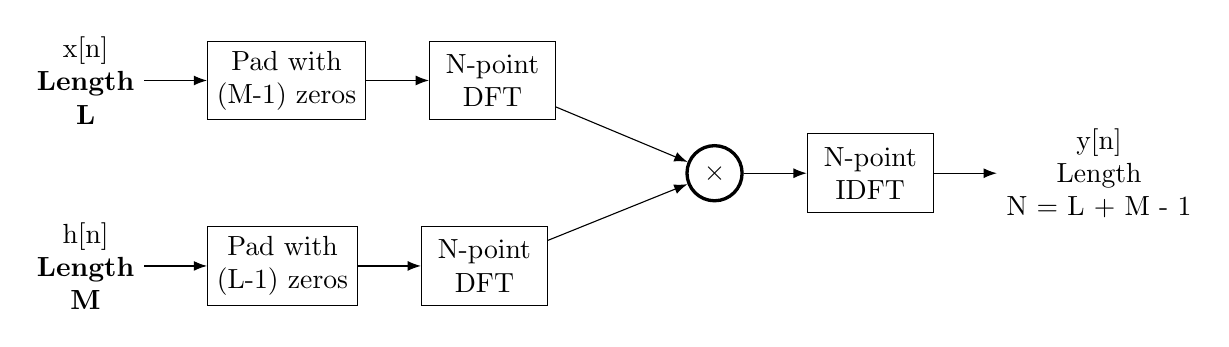
\begin{tikzpicture}[
  node distance=1cm and 0.8cm,
  box/.style={draw, minimum width=1.6cm, minimum height=1cm},
  arrow/.style={-Latex},
  roundnode/.style={circle, draw, very thick, minimum size=7mm},
]
    

% Nodes
\node[align=center] (n1) {x[n] \\ \textbf{Length} \\ \textbf{L}};
\node[align=center, box, right=of n1] (n2) {Pad with \\(M-1) zeros};
\node[align=center,box, right=of n2] (n3) {N-point \\DFT};
\node[align=center, below=of n1] (n4) {h[n] \\ \textbf{Length} \\ \textbf{M}};
\node[align=center,box, right=of n4] (n5) {Pad with \\(L-1) zeros};
\node[align=center,box, right=of n5] (n6) {N-point \\DFT};
%\node (n8) {Analog Output};
% Pointers
\path (n3) -- (n6) coordinate[midway] (mid);
\node[roundnode, right=2.5cm of mid] (n7) {$\times$};
\node[align=center,box, right=of n7] (n8) {N-point \\ IDFT};
\node[align=center, right=of n8] (n9) {y[n] \\ Length \\
N = L + M - 1};
% Arrows
\draw[arrow] (n1) -- (n2);
\draw[arrow] (n2) -- (n3);
\draw[arrow] (n4) -- (n5);
\draw[arrow] (n5) -- (n6);
\draw[arrow] (n3) -- (n7);
\draw[arrow] (n6) -- (n7);
\draw[arrow] (n7) -- (n8);
\draw[arrow] (n8) -- (n9);
\end{tikzpicture}
Given the linear convolution of x[n] (sequence length L = 5) and h[n] (sequence length M = 3), this can be expressed in matrix form as
\[
\begin{bmatrix}
   y[0] \\
    y[1]   \\
    y[2] \\
    y[3]   \\  
    y[4]   \\ 
    y[5]   \\ 
    y[6]   \\ 
\end{bmatrix}
\begin{bmatrix}
    x[0] & 0  & 0  \\
    x[1] & x[0]  & 0  \\
    x[2] & x[1]  & x[0]  \\
    x[3] & x[2]  & x[1]  \\
    x[4] & x[3]  & x[2]  \\
    0 & x[4]  & x[3]  \\
    0 & 0  & x[4]  \\
\end{bmatrix}=
\begin{bmatrix}
    h[0]   \\
    h[1]  \\
    h[2]   \\
\end{bmatrix}
\]
The output sequence y[n] has length N = M + L - 1 = 7 samples. When zero padding h[n], x[n] gets circular shifted downwards (L-1) times, starting from the first column. After zero padding h[n] we get the following results:
\[
\begin{bmatrix}
   y[0] \\
    y[1]   \\
    y[2] \\
    y[3]   \\  
    y[4]   \\ 
    y[5]   \\ 
    y[6]   \\ 
\end{bmatrix}
\begin{bmatrix}
    x[4] & x[3]  & x[2]  \\
    0 & x[4]  & x[3]  \\
    0 & 0  & x[4]  \\
    x[0] & 0  & 0  \\
    x[1] & x[0]  & 0  \\
    x[2] &x[1]  & x[0]  \\
    x[3] & x[2]  & x[1]  \\
\end{bmatrix}=
\begin{bmatrix}
    h[0]   \\
    h[1]  \\
    h[2]   \\
    0   \\
    0   \\
    0   \\
    0   \\
\end{bmatrix}
\]
Linear convolution cannot serve as a replacement for real time FIR filtering time as DFT algorithms need all input samples to be collected, and the input sequence can be too large, but it can be very effective in offline DSP, especially when the sequence is thousands of lengths long. 


\subsection{Overlap \& Add}
Let x(n) be an input sequence of a long duration and h(n) be a finite length sequence of length $L_2$. Let the sequence x(n) be divided into a set of subsequences, each having a finite length L, and let each subsequence be padded with $L_2-1$ zeros to make its length equal to $L+L_2-1$. Also, the sequence h(n) is padded with L - 1 zeros. This gives x(n):
\begin{center}
$x_1(n)=[x(0),x(1),...,x(L-1),{\underbrace{0,...0]}_{L_2-1}}$ \\
$x_2(n)=[x(L),x(L+1),...,x(2L-1),{\underbrace{0,...0]}_{L_2-1}}$ \\
$x_m(n)=[(x((m-1)L),(x((m-1)L+1),...,x(mL-1),{\underbrace{0,...0]}_{L_2-1}}$
\end{center}
The output of an FIR filter with impulse response h[n] of length
M = 3 to an input sequence x[n] with length L = 8 is given by
\begin{figure}
    \centering
    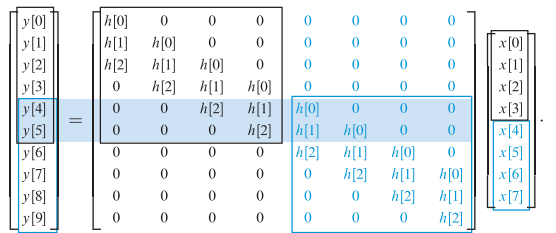
\includegraphics[width=1\linewidth]{OverlapAdd.png}
    \caption{Overlap-Add method with 2 blocks each with input length of 4. The impulse response gets zero padded with L-1 zeros}
\end{figure}
The black and blue correspond to the different blocks. The output of y[0]-y[5] corresponds to the black block and the output of y[4]-y[9] correspond to the blue block. In order to get the output of y[4] and y[5] you have to add the contributions from the blue and black blocks. Linear convolution of a length-L block with a length-M filter produces L + M - 1 output samples, the extra M - 1 samples produces the overlap, hence the term "Overlap and Add".
\subsection{Overlap \& Save}
In the overlap–add method, we need the output of the next
block to complete the computation of the current block. To avoid this drawback, we allow
successive input segments to overlap by (M - 1) samples. Overlap-Save is faster than Overlap-add for this reason
\begin{figure}[H]
    \centering
    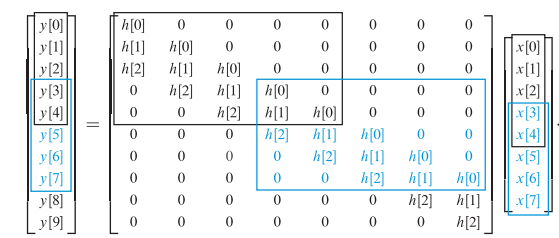
\includegraphics[width=1\linewidth]{OverlapSave.png}
\end{figure}
\subsection{Frequency Resolution}
The DFT works by correlating an input signal with sinusoids of different frequencies, and if the input signal correlates to one of these sinusoids, the correlation is nonzero. The formula for the frequency of fundamental sine and cosine used by the DFT for correlation with the fundamental frequency is
\begin{equation}
\Delta f=\frac{f_s}{N}, N = \text{number of samples of time signal}
\end{equation}
This is called the frequency resolution. If the input time-domain signal has two frequencies that are at least $\Delta f$, then the DFT is able to separate these two frequencies. Better frequency resolution can be achieved by increasing N and keeping $F_s$ or reducing the sampling rate but keeping N the same.
\begin{center}
Given two frequencies of 320 Hz and 640 Hz, if the sampling rate is 2560 and N = 512, the frequency resolution is \\
$$\Delta f = \frac{f_s}{N}=\frac{2650}{512}=5 \text{Hz}$$
\end{center}
Consider the 
\subsection{Fast Fourier Transform}
The FFT is essentially the DFT but the algorithm is manipulated to have less additions and multiplications, substantially reducing the computation of the DFT which has $O(N^2)$ complexity to $O(N\log N)$ complexity. Recall the periodocity property of the DFT states 
\begin{equation}
W_N^{kn}=W_N^{k(n+N)}=W_N^{(k+N)n}
\end{equation}
Recall $W_N=e^{-j2\pi/N}$. The symmetry property 
\begin{equation}
W_N^{kn+N/2}=-W_N^{kn}
\end{equation}
Taking the four-point DFT of an arbitrary signal yields 
\begin{center}
$$X(k)=\sum_{n=0}^{3}x(n)W_4^{nk},0 \leq k \leq 3;W_4=e^{-j2\pi/4}=-j$$
\end{center}
\[
\begin{bmatrix}
   X(0) \\
    X(1)  \\
    X(2)\\
    X(3)   
\end{bmatrix}=
\begin{bmatrix}
    W_4^0 & W_4^0  & W_4^0 & W_4^0  \\
   W_4^0 & W_4^1  & W_4^2 & W_4^3  \\
   W_4^0 & W_4^2  & W_4^4 & W_4^6  \\
   W_4^0 & W_4^3  & W_4^6 & W_4^9  \\
\end{bmatrix}
\begin{bmatrix}
    x(0) \\
    x(1)  \\
    x(2)\\
    x(3)   
\end{bmatrix}
\]
By periodicity: 
\begin{center}
$W_4^0=W_4^4=1$; \space \space $W_4^1=W_4^9=-j$; \\
\vspace{1em}
$W_4^2=W_4^6=-1$; \space \space $W_4^3=j$
\end{center}
Which yields the matrix
\[
\begin{bmatrix}
   X(0) \\
    X(1)  \\
    X(2)\\
    X(3)   
\end{bmatrix}=
\begin{bmatrix}
    1 & 1 & 1 & 1  \\
   1 & -j  & -1 & j  \\
   1& -1  & 1 & -1  \\
   1 & j  & -1 & -j  \\
\end{bmatrix}
\begin{bmatrix}
    x(0) \\
    x(1)  \\
    x(2)\\
    x(3)   
\end{bmatrix}
\]
\subsubsection{Decimation In Time radix-2 (Cooley-Tukey)}
Radix-2 means the number of output points N can be expressed as a power of 2. More simply, radix-2 involves decimating a DFT of length N by 2 in each stage of the DFT. This means that radix-2 performed on a 8 point sequence yields 3 stages where the input is split into two 4 point DFTs then two 2 point DFTs where the even samples of the signal are split from the odd samples of the signal.
\begin{figure}[H]
    \centering
    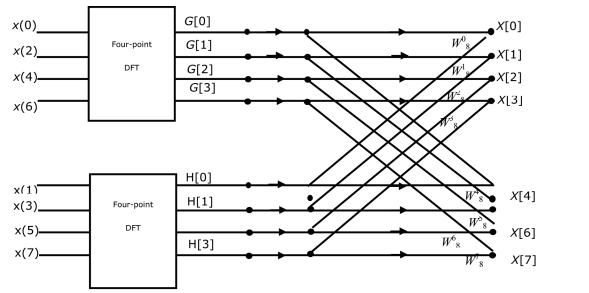
\includegraphics[width=1\linewidth]{DecimationInTime.png}
\end{figure}
Reviewing the DFT above, looking at the symmetry we see 
\begin{center}
$X(0) = x(0) + x(1) + x(2) + x(3) = [\underbrace{x(0)+x(2)}_{g_1}]+[\underbrace{x(1)+x(3)}_{g_2}]$ \\
$X(1) =  x(0) - jx(1) - x(2) + jx(3) = [\underbrace{x(0)-x(2)}_{h_1}]-j[\underbrace{x(1)-x(3)}_{h_2}]$ \\
$X(2) =  x(0) - x(1) + x(2) -x(3) = [\underbrace{x(0)+x(2)}_{g_1}]-[\underbrace{x(1)+x(3)}_{g_2}]$ \\
$X(3) =  x(0) + jx(1) - x(2) -jx(3) = [\underbrace{x(0)-x(2)}_{h_1}]+j[\underbrace{x(1)-x(3)}_{h_2}]$ \\
\end{center}
We see that 
\begin{center}
$g_1=x(0)+x(2)$ \\
$g_2=x(1)+x(3)$ \\
$h_1=x(0)-x(2)$ \\
$h_1=x(1)-x(3)$ \\
\end{center}
Which we can use to simplify X(k)
\begin{center}
$X(0) = g_1+g_2$\\
$X(1)=h_1-jh_2$\\
$X(2)=g_1-g_2$\\
$X(3)=h_1+jh_2$
\end{center}
We can see that a more efficient radix-2 FFT can be performed instead. We first split the even and odd samples into separate column vectors.
\begin{center}
\[
\begin{bmatrix}
   x(0) \\
    x(2)  \\
\end{bmatrix}
\begin{bmatrix}
   x(1) \\
    x(3)  \\
\end{bmatrix}=
\begin{bmatrix}
   x(0) & x(1) \\
    x(2) & x(3) \\
\end{bmatrix}
\]
We then perform a two-point DFT on each column
\[W_2
\begin{bmatrix}
   x(0) & x(1) \\
    x(2) & x(3) \\
\end{bmatrix}=
\begin{bmatrix}
   1 & 1 \\
    1 & -1 \\
\end{bmatrix}
\begin{bmatrix}
   x(0) & x(1) \\
    x(2) & x(3) \\
\end{bmatrix}=
\begin{bmatrix}
   x(0)+x(2) & x(1)+x(3) \\
    x(0)-x(2) & x(1)-x(3) \\
\end{bmatrix}=
\begin{bmatrix}
   g_1 & g_2 \\
    h_1 & h_2 \\
\end{bmatrix}
\]
\end{center}
Then each element of the resultant matrix is multiplied by $W_4^{pq}$ where p is the row index and q is the column index ($e^{(-j2\pi/N)pq}$), first row is 0, first column is 0. 
\[
\begin{bmatrix}
   W_N^0 & W_N^0  \\
    W_N^0  & W_N^1  \\
\end{bmatrix}\cdot
\begin{bmatrix}
   g_1 & g_2 \\
    h_1 & h_2 \\
\end{bmatrix}\Rightarrow
\begin{bmatrix}
   1 & 1  \\
    1  & -j  \\
\end{bmatrix}\cdot
\begin{bmatrix}
   g_1 & g_2 \\
    h_1 & h_2 \\
\end{bmatrix}=
\begin{bmatrix}
   g_1 & g_2 \\
    h_1 & -jh_2 \\
\end{bmatrix}
\]
Then finally take the 2 point DFT again
\[
\begin{bmatrix}
   g_1 & g_2 \\
    h_1 & -jh_2 \\
\end{bmatrix}W_2=
\begin{bmatrix}
   g_1 & g_2 \\
    h_1 & -jh_2 \\
\end{bmatrix}
\begin{bmatrix}
   1 & 1 \\
    1 & -1 \\
\end{bmatrix}=
\begin{bmatrix}
   g_1+g_2 & g_1-g_2 \\
    h_1-jh_2 & h_1+jh_2 \\
\end{bmatrix}=
\begin{bmatrix}
  X(0) & X(2) \\
    X(1) & X(3) \\
\end{bmatrix}
\]
\subsection{Differences between DFT and DTFT}
The DFT is a sampled version of the DTFT where $\omega$ is also sampled. The DFT and DTFT must be exactly the same at sampling intervals for them to produce the same result, that is the sample interval where k = 0,1,2,3,...N, must be:
\begin{equation}
\omega =\frac{2\pi}{N}
\end{equation}
For a signal x(n) with length N = 4, the sampling frequency is $\frac{\pi}{2}$. This means every $\omega=(\pi /2)N$ the DFT and DTFT yield the same result. 






\section{Filter Structures}
The filter design issue is influenced by such factors as the type of the filter (i.e., IIR or FIR) or the form of its implementation (structures). Hence, before we discuss the design issue, we first concern ourselves with how these filters can be implemented in practice. IIR filters as designed and used in DSP, can be modeled by rational system functions or, equivalently, by difference equations. Such filters are termed autoregressive moving average (ARMA) or, more generally, as recursive filters. Although ARMA filters include moving average filters that are FIR filters, we will treat FIR filters separately from IIR filters for both design and implementation purposes.

\subsection{Basic elements}
\begin{itemize}
    \item Adder: This element has two inputs and one output and is shown in
    Figure 6.1a. Note that the addition of three or more signals is implemented by successive two-input adders.
    \item Multiplier (gain): This is a single-input, single-output element and is
    shown in Figure 6.1b. Note that the multiplication by 1 is understood
    and hence not explicitly shown.
    \item Delay element (shifter or memory): This element delays the signal passing through it by one sample, as shown in Figure 6.1c. It is
    implemented by using a shift register.
    \begin{figure}[H]
        \centering
        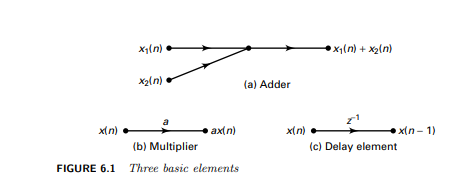
\includegraphics[width=0.5\linewidth]{Basic_elements.png}
        \label{fig:enter-label}
    \end{figure}
\end{itemize}
\subsection{IIR Filter structures}
The transfer function of an IIR filter is given by
\begin{equation}
H(z) = \frac{B(z)}{A(z)} = \frac{\sum_{n=0}^{M}b_nz^{-n}}{\sum_{n=0}^{N}a_nz^{-n}}= \frac{bo+b_1z^{-1}+...b_Mz^{-M}}{1+a_1z^{-1}+...a_Nz^{-N}};a_o=1
\end{equation}
The difference equation representation:
\begin{equation}
y(n) =  \sum_{m=0}^{M}b_mx(n-m) - \sum_{m=1}^{N}a_my(n-m) 
\end{equation}
where N is the order of the system
\subsubsection{Structures}
\begin{itemize}
    \item Direct form: In this form the difference equation is implemented directly as given. There are two parts to this filter, namely the moving average part and the recursive part (or equivalently, the numerator and denominator parts). Therefore this implementation leads to two versions: direct form I and direct form II structures.
    \item Cascade form: In this form the system function H(z) in equation
    (6.1) is factored into smaller 2nd-order sections, called biquads. The
    system function is then represented as a product of these biquads. Each
    biquad is implemented in a direct form, and the entire system function
    is implemented as a cascade of biquad sections. This is generally a more practical form for implementation because it has the least sensitivity to quantization, hence it will still be stable under quantization compared to other forms 
    \item Parallel form: This is similar to the cascade form, but after factorization, a partial fraction expansion is used to represent H(z) as a sum of smaller 2nd-order sections. Each section is again implemented in a direct form, and the entire system function is implemented as a parallel network of sections. This form is efficient when you have multiple CPUs, allowing the filter to be ran in parallel on multiple CPUs, but when you do not have a multicore processor this isn't a particularly useful form and is just pedagogical, just like Direct Form I.  

\end{itemize}
\newpage
\subsubsection{Direct Form}
Consider the difference equation
\begin{equation}
y(n) = b_0x(n) + b_1x(n - 1) + b_2x(n - 2) + b_3x(n - 3) + b_4x(n - 4)
- a_1y(n - 1) - a_2y(n - 2) - a_3y(n - 3) - a_4y(n - 4)    
\end{equation}

The corresponding Direct Form 1 Structure
\begin{figure}[H]
    \centering
    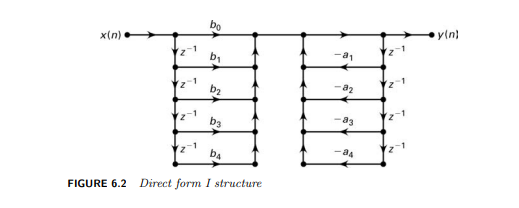
\includegraphics[width=1\linewidth]{Direct_Form1.png}
    \label{fig:enter-label}
\end{figure}
The corresponding Direct Form 2 Structure
\begin{figure}[H]
    \centering
    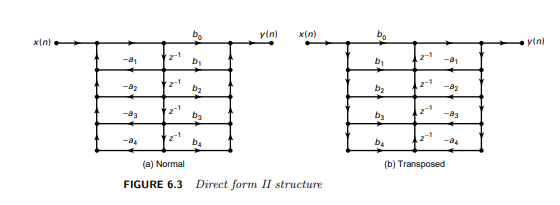
\includegraphics[width=1\linewidth]{DirectForm2.png}
    \label{fig:enter-label}
\end{figure}
In MATLAB the direct form structure is described by two row vectors;
b containing the {bn} coefficients and a containing the {an} coefficients.
The filter function, which is discussed in Chapter 2, implements the
transposed direct form II structure.

\newpage
\subsubsection{Cascade Form}
Cascade form is important for higher order systems. In cascade form, H(z) is written as the product of 2nd-order sections with real coefficients. This is done by factoring the numerator and denominator polynomials into their respective roots and then combining either a complex conjugate root pair or any two real roots into 2nd-order polynomials. \\

\vspace{1em}
Corresponding transfer function:
\begin{equation}
H(z) = b_o\prod_{k=1}^{K}\frac{1+B_{k,1}z^{-1}+B_{k,2}z^{-2}}{1+A_{k,1}z^{-1}+A_{k,2}z^{-2}}; k = 1,...,K
\end{equation}
where $\prod$ simply means multiplication. In this case, K corresponds to the multiplier, so K = 3 would imply 3 cascaded systems.

\vspace{1em}
Equivalent cascade form for above system
\begin{figure}[H]
    \centering
    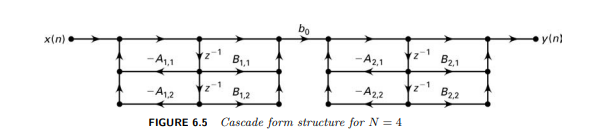
\includegraphics[width=1\linewidth]{Cascade.png}
    \caption{Enter Caption}
    \label{fig:enter-label}
\end{figure}
MATLAB implementation. The following program converts direct form to cascade form.
\begin{lstlisting}
function [b0,B,A] = dir2cas(b,a);
% DIRECT-form to CASCADE-form conversion (cplxpair version)
% ---------------------------------------------------------
% [b0,B,A] = dir2cas(b,a)
% b0 = gain coefficient
% B = K by 3 matrix of real coefficients containing bk's
% A = K by 3 matrix of real coefficients containing ak's
% b = numerator polynomial coefficients of DIRECT form
% a = denominator polynomial coefficients of DIRECT form
% compute gain coefficient b0
b0 = b(1); b = b/b0; a0 = a(1); a = a/a0; b0 = b0/a0;
%
M = length(b); N = length(a);
ifN>M
b = [b zeros(1,N-M)];   
elseif M > N
a = [a zeros(1,M-N)]; N = M;
else
NM = 0;
end
%
K = floor(N/2); B = zeros(K,3); A = zeros(K,3);
if K*2 == N;
b = [b 0]; a = [a 0];
end
%
broots = cplxpair(roots(b)); aroots = cplxpair(roots(a));
for i=1:2:2*K
Brow = broots(i:1:i+1,:); Brow = real(poly(Brow));
B(fix((i+1)/2),:) = Brow;
Arow = aroots(i:1:i+1,:); Arow = real(poly(Arow));
A(fix((i+1)/2),:) = Arow;
end
\end{lstlisting}
The following program implements cascade form
\begin{lstlisting}
function y = casfiltr(b0,B,A,x);
% CASCADE form realization of IIR and FIR filters
% -----------------------------------------------
%y= casfiltr(b0,B,A,x);
% y = output sequence
% b0 = gain coefficient of CASCADE form
% B = K by 3 matrix of real coefficients containing bk's
% A = K by 3 matrix of real coefficients containing ak's
% x = input sequence
%
[K,L] = size(B);
N = length(x); w = zeros(K+1,N); w(1,:) = x;
for i = 1:1:K
w(i+1,:) = filter(B(i,:),A(i,:),w(i,:));
end
y = b0*w(K+1,:);
\end{lstlisting}
The following program converts cascade form to direct form
\begin{lstlisting}
function [b,a] = cas2dir(b0,B,A);
% CASCADE-to-DIRECT form conversion
% ---------------------------------
% [b,a] = cas2dir(b0,B,A)
% b = numerator polynomial coefficients of DIRECT form
% a = denominator polynomial coefficients of DIRECT form
% b0 = gain coefficient
% B = K by 3 matrix of real coefficients containing bk's
% A = K by 3 matrix of real coefficients containing ak's
%
[K,L] = size(B);
b = [1]; a = [1];
for i=1:1:K
b=conv(b,B(i,:)); a=conv(a,A(i,:));
end
b = b*b0;    
\end{lstlisting}
Example: \\
Determine the cascaded form structure of the filter with the following difference equation: 
\begin{equation}
16y(n) + 12y(n - 1) + 2y(n - 2) - 4y(n - 3) - y(n - 4)
= x(n) - 3x(n - 1) + 11x(n - 2) - 27x(n - 3) + 18x(n - 4)
\end{equation}

\begin{lstlisting}
 b=[1 -3 11 -27 18]; a=[16 12 2 -4 -1];
 [b0,B,A]=dir2cas(b,a)
Output:
b0 = 0.0625
B =
1.0000 -0.0000 9.0000
1.0000 -3.0000 2.0000
A =
1.0000 1.0000 0.5000
1.0000 -0.2500 -0.1250

%Verify correctness
 delta = impseq(0,0,7)
delta =
10000000
 format long
 hcas=casfiltr(b0,B,A,delta)
Output:
hcas =
Columns 1 through 4
0.06250000000000 -0.23437500000000 0.85546875000000 -2.28417968750000
Columns 5 through 8
2.67651367187500 -1.52264404296875 0.28984069824219 0.49931716918945
 hdir=filter(b,a,delta)
hdir =
Columns 1 through 4
0.06250000000000 -0.23437500000000 0.85546875000000 -2.28417968750000
Columns 5 through 8
2.67651367187500 -1.52264404296875 0.28984069824219 0.49931716918945
\end{lstlisting}
\begin{figure}[H]
    \centering
    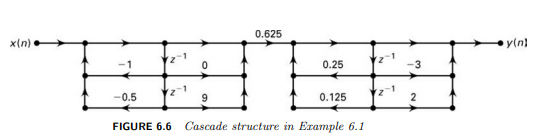
\includegraphics[width=1\linewidth]{Cascade2.png}
    \label{fig:enter-label}
\end{figure}
\subsubsection{Parallel form}
In this from, H(z) is written as a sum of 2nd-order sections using partial fraction expansion
\begin{equation}
H(z) = \frac{B(z)}{A(z)}=\sum_{k=1}^{K}\frac{B_{k,0}+B_{k,1}z^{-1}}{A_{k,0}+A_{k,1}z^{-1}} + \sum_{0}^{M-N}C_k{z^{-k}}
\end{equation}
The below figure depcits parallel form realization.
\begin{figure}[H]
    \centering
    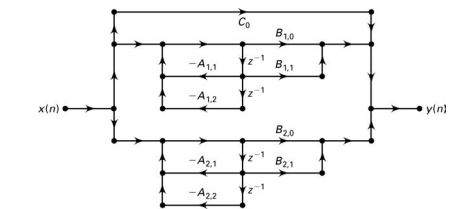
\includegraphics[width=1\linewidth]{Parallel.png}
    \caption{Parallel form structure for N=4}
    \label{fig:enter-label}
\end{figure}
The following function dir2par converts the direct-form coefficients {bn}
and {an} into parallel form coefficients {Bk,i} and {Ak,i}
\begin{lstlisting}
function [C,B,A] = dir2par(b,a);
% DIRECT-form to PARALLEL-form conversion
% --------------------------------------
% [C,B,A] = dir2par(b,a)
% C = Polynomial part when length(b) >= length(a)
% B = K by 2 matrix of real coefficients containing bk's
% A = K by 3 matrix of real coefficients containing ak's
% b = numerator polynomial coefficients of DIRECT form
% a = denominator polynomial coefficients of DIRECT form
%
M = length(b); N = length(a);
[r1,p1,C] = residuez(b,a);
p = cplxpair(p1,10000000*eps); I = cplxcomp(p1,p); r = r1(I);
K = floor(N/2); B = zeros(K,2); A = zeros(K,3);
if K*2 == N; %N even, order of A(z) odd, one factor is first order
for i=1:2:N-2
Brow = r(i:1:i+1,:); Arow = p(i:1:i+1,:);
[Brow,Arow] = residuez(Brow,Arow,[]);
B(fix((i+1)/2),:) = real(Brow); A(fix((i+1)/2),:) = real(Arow);
end
[Brow,Arow] = residuez(r(N-1),p(N-1),[]);
B(K,:) = [real(Brow) 0]; A(K,:) = [real(Arow) 0];
else
for i=1:2:N-1    
Brow = r(i:1:i+1,:); Arow = p(i:1:i+1,:);
[Brow,Arow] = residuez(Brow,Arow,[]);
B(fix((i+1)/2),:) = real(Brow); A(fix((i+1)/2),:) = real(Arow);
end
end
\end{lstlisting}
The following function is used for complex conjugate pole pairs (after calling cplxpair).
\begin{lstlisting}
function I = cplxcomp(p1,p2)
% I = cplxcomp(p1,p2)
% Compares two complex pairs which contain the same scalar elements
% but (possibly) at differrent indices. This routine should be
% used after CPLXPAIR routine for rearranging pole vector and its
% corresponding residue vector.
% p2 = cplxpair(p1)
%
I=[];
for j=1:1:length(p2)
for i=1:1:length(p1)
if (abs(p1(i)-p2(j)) < 0.0001)
I=[I,i];
end
end
end
I=I';
\end{lstlisting}
The following function implements parallel form
\begin{lstlisting}
function y = parfiltr(C,B,A,x);
% PARALLEL form realization of IIR filters
% ----------------------------------------
% [y] = parfiltr(C,B,A,x);
% y = output sequence
% C = polynomial (FIR) part when M >= N
% B = K by 2 matrix of real coefficients containing bk's
% A = K by 3 matrix of real coefficients containing ak's
% x = input sequence
%
[K,L] = size(B); N = length(x); w = zeros(K+1,N);
w(1,:) = filter(C,1,x);
for i = 1:1:K
w(i+1,:) = filter(B(i,:),A(i,:),x);
end
y = sum(w);    
\end{lstlisting}
The following function converts parallel form to direct form
\begin{lstlisting}
function [b,a] = par2dir(C,B,A);
% PARALLEL-to-DIRECT form conversion
% ----------------------------------
% [b,a] = par2dir(C,B,A)
% b = numerator polynomial coefficients of DIRECT form
% a = denominator polynomial coefficients of DIRECT form
% C = Polynomial part of PARALLEL form
% B = K by 2 matrix of real coefficients containing bk's
% A = K by 3 matrix of real coefficients containing ak's
%
[K,L] = size(A); R = []; P = [];
for i=1:1:K
[r,p,k]=residuez(B(i,:),A(i,:)); R = [R;r]; P = [P;p];
end
[b,a] = residuez(R,P,C); b = b(:)'; a = a(:)';    
\end{lstlisting}
Determine the parallel form structure of the filter with the following difference equation: 
\begin{equation}
16y(n) + 12y(n - 1) + 2y(n - 2) - 4y(n - 3) - y(n - 4)
= x(n) - 3x(n - 1) + 11x(n - 2) - 27x(n - 3) + 18x(n - 4)
\end{equation}
\begin{lstlisting}
 b=[1 -3 11 -27 18]; a=[16 12 2 -4 -1];
 [C,B,A]=dir2par(b,a)
Output:
C =
-18
B =
10.0500 -3.9500
28.1125 -13.3625
A =
1.0000 1.0000 0.5000
1.0000 -0.2500 -0.1250    
\end{lstlisting}

\subsection{FIR Filter structures}
A finite-duration impulse response filter has a system function of the form
\begin{equation}
H(z) = b_0+b_1z^{-1}+...+b_{M-1}z^{1-M}=\sum_{n=0}^{M-1}b_nz^{-n}
\end{equation}
hence the impulse response h(n) is 
\begin{equation}
h(n) = \begin{cases}
b_n , &  0 \leq n \leq M - 1 \\
0, & else
\end{cases}
\end{equation}
The difference equation representation:
\begin{equation}
y(n) = b_0x(n) + b_1x(n-1) +...b_{M-1}x(n-M+1)
\end{equation}
\subsubsection{Structures}
\begin{itemize}
    \item Direct form: In this form the difference equation (6.7) is implemented directly as given.
    \item Cascade form: In this form the system function H(z) in (6.5) is factored into 2nd-order factors, which are then implemented in a cascade connection.
    \item Linear-phase form: When an FIR filter has a linear-phase response,
    its impulse response exhibits certain symmetry conditions. In this form
    we exploit these symmetry relations to reduce multiplications by about
    half. 
    \item Frequency-sampling form: This structure is based on the DFT of
    the impulse response h(n) and leads to a parallel structure. It is also
    suitable for a design technique based on the sampling of frequency
    response $H(e^{jw})$.
\end{itemize}
\newpage
\subsubsection{Direct Form}
The below figure is the model for Direct form FIR structure
\begin{figure}[H]
    \centering
    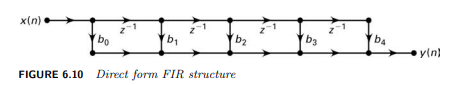
\includegraphics[width=1\linewidth]{DirectFIR.png}
    \label{fig:enter-label}
\end{figure}
This can be represented by the equation:
\begin{equation}
y(n) = b_0x(n) + b_1x(n - 1) + b_2x(n - 2) + b_3x(n - 3) + b_4x(n - 4)    
\end{equation}
\subsubsection{Cascade form}
\begin{equation}
H(z) = b_o\prod_{k=1}^{K}(1+B_{k,1}z^{-1}+B_{k,2}z^{-2})
\end{equation}
\begin{figure}[H]
    \centering
    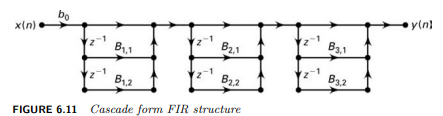
\includegraphics[width=1\linewidth]{CascadeFIR.png}
    \label{fig:enter-label}
\end{figure}
\subsubsection{Linear-Phase Form}
For frequency-selective filters (e.g., lowpass filters) it is generally desirable to have a phase response that is a linear function of frequency; that is, we want
\begin{equation}
\angle H(jw) = \beta - \alpha\omega, -\pi < \omega \leq \pi
\end{equation}
where $\beta$ is 0 or $\pm \frac{\pi}{2}$ and $\alpha$ is constant.
For a causal FIR filter with
impulse response over [0, M - 1] interval, the linear-phase condition imposes the conditions
\begin{center}
$h(n) = h(M - 1 - n)$; $\beta = 0, \alpha= \frac{M-1}{2},0 \leq n \leq\ M - 1$ \\
\vspace{1em}
$h(n) = -h(M - 1 - n)$; $\beta = \pm \frac{\pi}{2}, \alpha= \frac{M-1}{2},0 \leq n \leq\ M - 1$
\end{center}
An impulse resonse that satisifies  $h(M - 1 - n)$ is a symmetric impulse response, and one that satisfies  $-h(M - 1 - n)$ is an antisymmetric impulse response.
\newpage
Difference equation form
\begin{equation}
y(n) = b_0x(n) + b_1x(n - 1) + ... + b_1x(n - M + 2) + b_0x(n - M + 1)
= b_0[x(n) + x(n - M + 1)] + b_1[x(n - 1) + x(n - M + 2)] + \cdots
\end{equation}
FIR Linear-Phase Structure 
\begin{figure}[H]
    \centering
    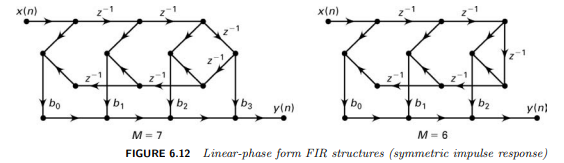
\includegraphics[width=1\linewidth]{LinearPhase.png}
    \label{fig:enter-label}
\end{figure}
An FIR filter is given by the system function
\begin{equation}
H(z) = 1 + 16.0625z^{-4}+z^{-8}
\end{equation}
Direct form difference equation: \\
$y(n) = x(n) + 16.0625x(n - 4) + x(n - 8)$ \\
Linear-phase: \\
$y(n)=[x(n) + x(n - 8)] + 16.0625x(n - 4)$ \\
\begin{figure}[H]
    \centering
    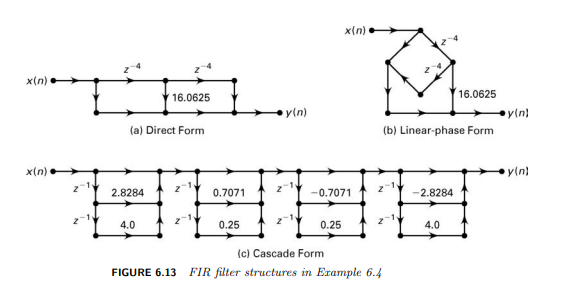
\includegraphics[width=1\linewidth]{Systemcompared.png}
    \label{fig:enter-label}
\end{figure}

\subsection{Lattice Filters (unfinished)}
Used for speech processing

\subsection{Block Diagram of Time Domain}
\begin{figure}[H]
    \centering
    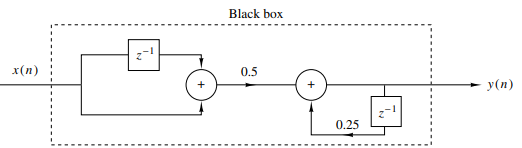
\includegraphics[width=1\linewidth]{BlockDiagram1.png}
    \caption{Block diagram realization of system $y(n)=0.25y(n-1)+0.5x(n)+0.5x(n-1)$}
\end{figure}
\subsection{Signal Flow Graph}
\begin{figure}[H]
    \centering
    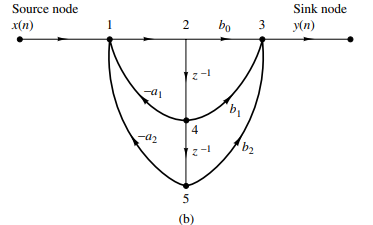
\includegraphics[width=1\linewidth]{SignalFlow1.png}
\end{figure}
\section{Time Series denoising}
\subsection{Mean Smoothing Filter}
Essentially smooths a time domain signal based on the averages of the points around a adjacent time points.
\begin{equation}
y_t=(2k+1)^{-1}\sum_{i=t-k}^{t+k}x_i
\end{equation}
Where $y_t$ is the filtered signal

\begin{lstlisting}
% create signal
srate = 1000; % Hz 
time = 0:1/srate:3;
n = length(time);
p = 15; %poles for random interpolation 

% noise level measured in standard deviations 
noiseamp = 5;

% amplitude modulator and noise level 
amp = interp1(rand(p,1)*30,linspace(1,p,n));
noise = noiseamp * randn(size(time));
signal = ampl + noise;

% initialize filtered signal vector
fitlsig = zeros(size(signal));

% implement the running mean filter 
k = 20; % filter window is actually k*2 + 1
for i=k+1:n-k-1
% each point is the average of k surrounding points 
filtsig(i) = mean(signal(i-k:i+k));
end 

% plot the noisy and filtered signals 
figure(1), clf, hold on 
plot(time, signal, time filtsig, 'linew',2)

% draw a patch to indicate the window size 
tidx = dsearchn(time',1);
ylin = get(gca, 'ylim');
patch(time([tidx-k tidx-k tidx +k tidx+k ]), ylim([1 2 2 1]), 'k', 'facealpha',.2)
plot(time([tidx tidx], ylim 'k--')


\end{lstlisting}

\section{Time-Frequency Analysis}
\subsection{Transforms for Time-Frequency}
\subsubsection{Short  Time Fourier Transform}
Suppose you wish to determine the spectral contents (the frequencies) of a certain
sound y(t) during the time interval $1 \leq t \leq 2$ A simple idea would be to compute the Fourier transform of y(t) from t = 1 to t = 2 instead of %t = -\infty$
to $t = \infty$ however this is problematic based on how the FT interprets the corners so large and undesired spectral high frequency. contents would appear. The problem can be mitigated introducing a smooth ‘window
function’ w(t - tc) covering the time interval of interest. The equation for STFT: 
\begin{equation}
F_y(t,w) = \int_{-\infty}^{\infty}y(\tau)w(\tau-t)e^{-j\omega \tau}d\tau
\end{equation}

\section{FIR Filter Design: The Theory}
\subsection{Preliminaries}
Generally, a linear phase response in the passband is desirable. In the case of FIR filters, it is possible to have exact linear phase, as we have seen in Chapter 6. In the case of
IIR filters, a linear phase in the passband is not achievable. Hence IIR
considers magnitude-only specifications. For FIR filter design, absolute specifications are considered. 

\subsubsection{Absolute specifications}
A typical absolute specification of a lowpass filter is shown in Figure 7.1a,
in which

\begin{itemize}
    \item band [0, $w_p$] is called the passband and  $\delta_1$ is the tolerance (or ripple) that we are willing to accept in the ideal passband response,
    \item  band [$w_s$, $\pi$] is called the stopband and $\delta_2$ is the corresponding tolerance (or ripple), and \\
    \item band [$w_p$, $w_s$] is called the transition band that imposes no restrictions \\
\end{itemize}
on the magnitude response.

\begin{figure}[H]
    \centering
    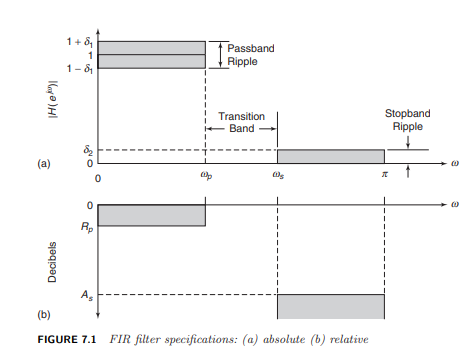
\includegraphics[width=1\linewidth]{specificationsFIR.png}

    \label{fig:enter-label}
\end{figure}

\subsubsection{Relative specifications}
A typical relative specification of a lowpass filter is shown in Figure 7.1b,
in which \\
• Rp is the passband ripple in dB, and \\
• As is the stopband attenuation in dB.
\begin{equation}
R_p=-20log_{10}\frac{1-\delta_1}{1+\delta_1} > 0 
\end{equation}
\begin{equation}
A_s=-20log_{10}\frac{\delta_2}{1+\delta_1} > 0
\end{equation}
\vspace{1em}
Given the passband tolerance $\delta_1$ = 0.01 and the stopband tolerance $\delta_2$ = 0.001,
determine the passband ripple $R_p$ and the stopband attenuation $A_s$.
\vspace{1em}
\begin{center}
$R_p=-0.20log_{10}\frac{1-\delta_1}{1+\delta_1}=0.1737$ dB \\
\vspace{1em}
$A_s=-20log_{10}\frac{\delta_2}{1+\delta_1} = 60$ dB
\end{center} 
\vspace{1em}
These specifications were given for a lowpass filter. Similar specifications can also be given for other types of frequency-selective filters, such
as highpass or bandpass. However, the most important design parameters are frequency-band tolerances (or ripples) and band-edge frequencies.
Whether the given band is a passband or a stopband is a relatively minor
issue. Therefore, in describing design techniques, we will concentrate on
a lowpass filter. 

\subsubsection{Advantages of FIR}
Advantages:
\begin{itemize}
    \item The phase response can be exactly linear.
    \item They are relatively easy to design since there are no stability problems
    \item They are efficient to implement
    \item The DFT can be used in their implementation.
    \item The design problem contains only real arithmetic and not complex arithmetic
    \item Linear-phase filters provide no delay distortion and only a fixed amount of delay
    \item For the filter of length M (or order M - 1), the number of operations are of the order of M/2, as we discussed in the linear-phase filter implementation

\end{itemize}
\subsubsection{IIR vs FIR}
FIR filters are preferred when linear phase is important and stability is a concern. IIR filters are used when a sharp frequency response is needed with low computational cost, even at the expense of phase linearity and some stability considerations. \\
\vspace{1em}
When FIR is better than IIR is better 
\begin{itemize}
    \item Exact linear phase: FIR filters can be designed to have exact linear phase, which is vital in audio, data transmission, and image processing to avoid phase distortion.
    \item Stability: FIR filters are always stable because they don't use feedback.
    \item Finite impulse response: FIR filters have a finite response, making them easier to analyze and implement in some hardware systems.
    \item Simple implementation: Easier to implement on fixed-point DSP hardware because there's no recursion.
    \item Multirate (sampling rate conversion): They're preferred in interpolation, decimation, and  multirate DSP systems for their inherent stability.
\end{itemize}
When IIR filter is better
\begin{itemize}
    \item Efficiency (lower order): IIR filters generally achieve a given frequency response with a much lower order (fewer coefficients), so they're more computationally efficient for the same level of sharpness in magnitude response.
    \item Analog filter emulation: IIR designs (like Butterworth, Chebyshev, Elliptic) can directly map analog filter designs (prototype-based) to digital equivalents — this is useful in control systems and analog-replacement designs.
    \item Sharp transitions: When you need a very narrow transition band (e.g., in telecommunications channel filters), IIR filters typically outperform FIR filters of the same order.
\end{itemize}

\newpage
\subsection{Properties of Linear-Phase FIR Filters}
In this section, we discuss shapes of impulse and frequency responses and
locations of system function zeros of linear-phase FIR filters. Let h(n),
$0 \leq n \leq M - 1$, be the impulse response of length (or duration) M. Then
the system function is

\begin{equation}
    H(z) = \sum_{n=0}^{M-1}h(n)z^{-n} = z^{-(M-1)}\sum_{n=0}^{M-1}h(n)z^{M-1-n}
\end{equation}
which has (M - 1) poles at the origin z = 0 (trivial poles) and (M - 1)
zeros located anywhere in the z-plane. The frequency response function
is
\begin{equation}
    H(e^{jw})=\sum_{n=0}^{M-1}h(n)e^{-jwn}, -\pi < \omega \leq \pi
\end{equation}

\subsubsection{Impulse response}
\begin{figure}[H]
    \centering
    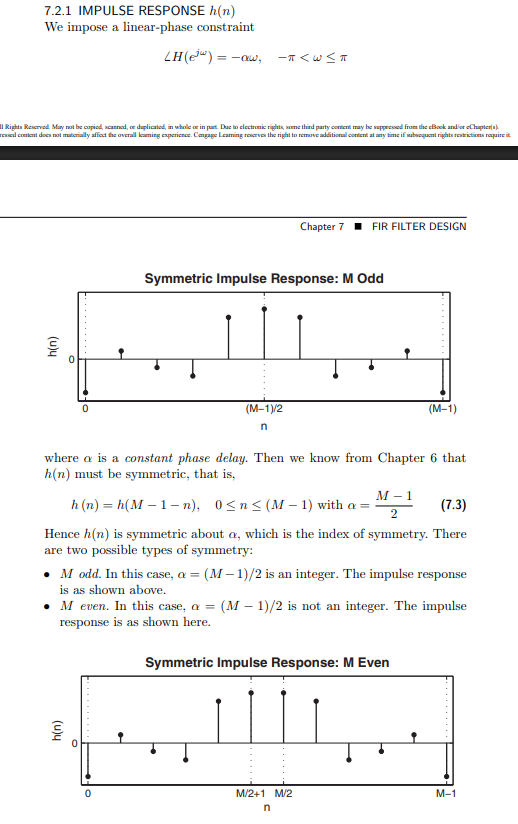
\includegraphics[width=0.75\linewidth]{SymmetricImpulseFIR.png}
    \label{fig:enter-label}
\end{figure}
\begin{figure}[H]
    \centering
    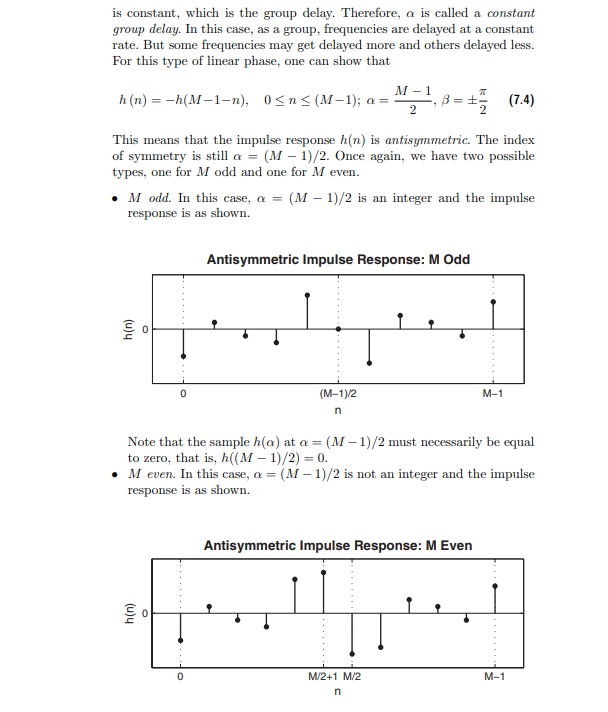
\includegraphics[width=1\linewidth]{AssymetricImpulseFIR.png}
    \label{fig:enter-label}
\end{figure}

\subsubsection{Frequency Response}
General equation:
\begin{equation}
H(e^{jw}) = H_r(w)e^{j(\beta-\alpha w)}; \beta= \pm\frac{\pi}{2}, \alpha= \frac{M-1}{2}
\end{equation}
Where $H_r(w)$ is an amplitude response function and not a magnitude response function. The amplitude response is a real function, but unlike
the magnitude response, which is always positive, the amplitude response
may be both positive and negative.The phase response associated with
the magnitude response is a discontinuous function, while that associated
with the amplitude response is a continuous linear function. \\
\vspace{1em}

Let Let the impulse response be $h(n) = {1, 1, 1}$. Determine and draw frequency responses
\begin{center}
$H(e^{jw})=\sum_0^2h(n)e^{jw}=1+1e^{-jw}+e^{-j2w}= e^{-jw}({e^{jw}+1+e^{-jw}})=$ \\
\vspace{1em}
$= e^{-jw}(1+2cosw)$
\end{center}
Magnitude and phase responses
\begin{center}
$|H(e^{jw})|=|1+2cosw|, 0,w \leq \frac{2\pi}{3}$ \\
\vspace{1em}
$\angle H(e^{jw})= \begin{cases}
-w, & 0 < w < 2\pi/3 \\
\pi -w, & 2\pi/3 < w < \pi
\end{cases}$
Phase response and amplitude responses 
\begin{center}
$H_r(w)=1+2cosw$ \\
$\angle H(e^{jw}) = -w$
\end{center}
\begin{figure}[H]
    \centering
    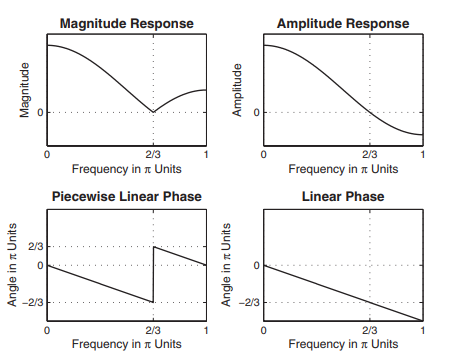
\includegraphics[width=1\linewidth]{AmplitudePhaseMagnitudeFIR.png}
    \label{fig:enter-label}
\end{figure}
\end{center}
\newpage
\subsubsection{Linear-phase type Frequency Responses}
\begin{enumerate}
    \item Symmetrical Impulse Response, M odd (Type 1)
    \begin{center}
        $$H(e^{jw})=[\sum_{n=0}^{(M-1)/2}a(n)\cos\omega n ]e^{-jw(M-1)/2}$$ \\
        \vspace{1em}
        $$a(n) = 2h(\frac{M-1}{2}-n), 1 \leq n \leq \frac{M-3}{2}$$ \\
        \vspace{1em}
        $$H_r(w)=\sum_{n=0}^{(M-1)/2}a(n)\cos\omega n$$
    \end{center}
    \item Symmetrical Impulse Response, M even (Type 2)
    \begin{center}
        $$H(e^{jw})=[\sum_{n=1}^{M/2}b(n)\cos(\omega( n-\frac{1}{2})) ]e^{-jw(M-1)/2}$$ \\
        \vspace{1em}
        $$b(n) = 2h(\frac{M}{2}-n), n = 1, 2,...,\frac{M}{2}$$ \\
        \vspace{1em}
        $$H_r(w)=\sum_{n=0}^{M/2}b(n)\cos(\omega(n-\frac{1}{2}))$$
    \end{center}
    \item Antisymmetric impulse response, M odd (Type 3)
    \begin{center}
        $$H(e^{jw})=[\sum_{n=1}^{(M-1)/2}c(n)\sin\omega n ]e^{j[\frac{\pi}{2}-(\frac{M-1}{2})\omega]}$$ \\
        \vspace{1em}
        $$c(n) = 2h(\frac{M-1}{2}-n), n = 1, 2,...,\frac{M-1}{2}$$ \\
        \vspace{1em}
        $$H_r(w)=\sum_{n=0}^{(M-1)/2}c(n)\sin\omega n$$
    \end{center}
    \item Antisymmetric impulse response, M even (Type 4)
    \begin{center}
        $$H(e^{jw})=[\sum_{n=1}^{M/2}d(n)\sin(\omega (n - \frac{1}{2}))]e^{j[\frac{\pi}{2}-\omega{(M-1)}/{2})]}$$ \\
        \vspace{1em}
        $$d(n) = 2h(\frac{M}{2}-n), n = 1, 2,...,\frac{M}{2}$$ \\
        \vspace{1em}
        $$H_r(w)=\sum_{n=0}^{M/2}d(n)\sin(\omega( n-\frac{1}{2}))$$
    \end{center}
    
\end{enumerate}
\begin{enumerate}
    \item Hr\_type1
\begin{lstlisting}
function [Hr,w,a,L] = Hr_Type1(h);
% Computes amplitude response Hr(w) of a Type-1 LP FIR filter
% -----------------------------------------------------------
% [Hr,w,a,L] = Hr_Type1(h)
% Hr = amplitude response
% w = 500 frequencies between [0 pi] over which Hr is computed
% a = type-1 LP filter coefficients
% L = order of Hr
% h = type-1 LP filter impulse response
%
M = length(h); L = (M-1)/2;
a = [h(L+1) 2*h(L:-1:1)]; % 1x(L+1) row vector
n = [0:1:L]; % (L+1)x1 column vector
w = [0:1:500]'*pi/500; Hr = cos(w*n)*a';

\end{lstlisting}
    \item Hr\_type2
    \begin{lstlisting}
    function [Hr,w,b,L] = Hr_Type2(h);
% Computes amplitude response of a Type-2 LP FIR filter
% -----------------------------------------------------
% [Hr,w,b,L] = Hr_Type2(h)
% Hr = amplitude response
% w = frequencies between [0 pi] over which Hr is computed
% b = type-2 LP filter coefficients
% L = order of Hr
% h = type-2 LP impulse response
%
M = length(h); L = M/2;
b = 2*[h(L:-1:1)]; n = [1:1:L]; n = n-0.5;
w = [0:1:500]'*pi/500; Hr = cos(w*n)*b';
        
    \end{lstlisting}
    \item Hr\_type3
    \begin{lstlisting}
function [Hr,w,c,L] = Hr_Type3(h);
% Computes amplitude response Hr(w) of a Type-3 LP FIR filter
% -----------------------------------------------------------
% [Hr,w,c,L] = Hr_Type3(h)
% Hr = amplitude response
% w = frequencies between [0 pi] over which Hr is computed
% c = type-3 LP filter coefficients
% L = order of Hr
% h = type-3 LP impulse response
%
M = length(h); L = (M-1)/2;
c = [2*h(L+1:-1:1)]; n = [0:1:L];
w = [0:1:500]'*pi/500; Hr = sin(w*n)*c';

        
    \end{lstlisting}
    \item Hr\_type4
    \begin{lstlisting}
    function [Hr,w,d,L] = Hr_Type4(h);
% Computes amplitude response of a Type-4 LP FIR filter
% -----------------------------------------------------
% [Hr,w,d,L] = Hr_Type4(h)
% Hr = amplitude response
% w = frequencies between [0 pi] over which Hr is computed
% d = type-4 LP filter coefficients
% L = order of d
% h = type-4 LP impulse response
%
M = length(h); L = M/2;
d = 2*[h(L:-1:1)]; n = [1:1:L]; n = n-0.5;
w = [0:1:500]'*pi/500; Hr = sin(w*n)*d';
        
    \end{lstlisting}


\end{enumerate}
These four functions can be combined into one function, called
ampl res, that can be written to determine the type of the linear-phase
filter and to implement the appropriate amplitude response expression.
This is explored in Problem P7.6. The use of these functions is described
in Examples 7.4 through 7.7.
The zerophase function from the SP toolbox is similar in use to the
freqz function. The invocation [Hr,w, phi] = zerophase(b,a) returns
the amplitude response in Hr, evaluated at 512 values around the top half
of the unit circle in the array w and the continuous phase response in
phi. Thus this function can be used for both FIR and IIR filters. Other
invocations are also available

\subsubsection{Zeroes (unfinished)}




















\newpage










\subsection{Window Design Technique}
The basic idea behind the window design is to choose a proper ideal
frequency-selective filter (which always has a noncausal, infinite-duration
impulse response) and then to truncate (or window) its impulse response
to obtain a linear-phase and causal FIR filter. Therefore, the emphasis
in this method is on selecting an appropriate windowing function and
an appropriate ideal filter. We will denote an ideal frequency-selective
filter by $H_d(e^{jw})$, which has a unity magnitude gain and linear-phase
characteristics over its passband, and zero response over its stopband. An
ideal LPF of bandwidth $w_c < \pi$ is given by 
\begin{equation}
H_d(e^{jw})=\begin{cases}
    1*e^{-j\alpha\omega}, & |w| \leq w_c \\
    0, & w_c < |w| \leq \pi
\end{cases}
\end{equation}
Using Fourier techniques, the impulse response is
\begin{equation}
h_d(n) = \frac{\sin|(\omega_c(n-\alpha)|}{\pi(n-\alpha)}
\end{equation}
To obtain an FIR filter from $h_d(n)$, one has to truncate $h_d(n)$ on both
sides. To obtain a causal and linear-phase FIR filter h(n) of length M, we
must have
\begin{equation}
h(n) = \begin{cases}
h_d(n), & 0 \leq n \leq M-1 \\
0, & \textit{elsewhere} 
\end{cases}
\end{equation}
\begin{equation}
\alpha = \frac{M-1}{2}
\end{equation}
This operation is called “windowing.” In general, h(n) can be thought of
as being formed by the product of $h_d(n)$ and a window function w(n) as
follows:
\begin{equation}
    h(n)=h_d(n)w(n)
\end{equation}
where 
\begin{center}
$w(n)=$  $\begin{cases}
\textit{some symmetric function with respect to $\alpha$ over $0 \leq n \leq M -1$} \\
0, otherwise
\end{cases}$
\end{center}
\begin{figure}[H]
    \centering
    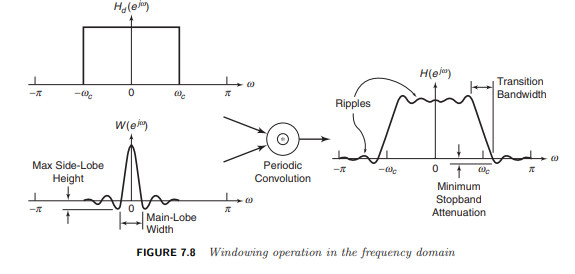
\includegraphics[width=1\linewidth]{WindowingOperation.png}
    \label{fig:enter-label}
\end{figure}
Basic window design idea: For the given filter specifications, choose
the filter length M and a window function w(n) for the narrowest mainlobe width and the smallest side-lobe attenuation possible

\subsubsection{Rectangular Window}
This is the simplest window function but provides the worst performance
from the viewpoint of stopband attenuation. It was defined earlier by
\begin{equation}
w(n) = \begin{cases}
    1, 0 \leq n \leq M -1 \\
    0, \text{otherwise}
\end{cases}
\end{equation}
In addition, the transition bandwith is $w_s-w_p = \frac{1.8\pi}{M}$  
\begin{figure}[H]
    \centering
    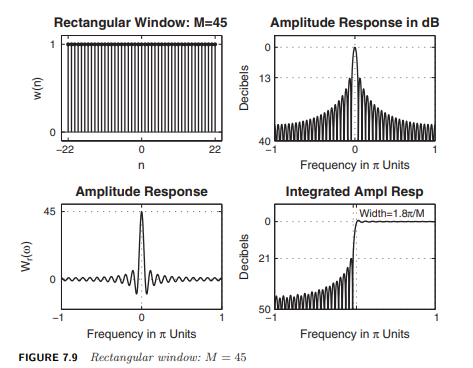
\includegraphics[width=1\linewidth]{RectangularWindow.png}
    \label{fig:enter-label}
\end{figure}
If we increase M, the width of each side lobe will
decrease, but the area under each lobe will remain constant. Therefore, the
relative amplitudes of side lobes will remain constant, and the minimum
stopband attenuation will remain at 21 dB. This implies that all ripples
will bunch up near the band edges.
\begin{figure}[H]
    \centering
    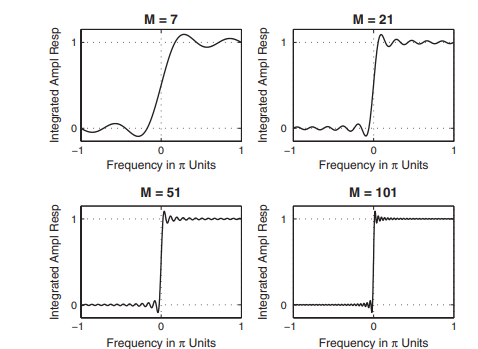
\includegraphics[width=1\linewidth]{MRelationToWindow.png}
    \label{fig:enter-label}
\end{figure}
\subsubsection{Bartlett Window}
Since the Gibbs phenomenon results from the fact that the rectangular
window has a sudden transition from 0 to 1 (or 1 to 0), Bartlett suggested
a more gradual transition in the form of a triangular window, which is
given by
\begin{equation}
w(n) = \begin{cases}
\frac{2n}{M-1}, & 0\leq n \leq \frac{M-1}{2} \\
2-\frac{2n}{M-1}, &\frac{M-1}{2} \leq n \leq M-1 \\
0, \text{otherwise}
\end{cases}
\end{equation}
\begin{figure}[H]
    \centering
    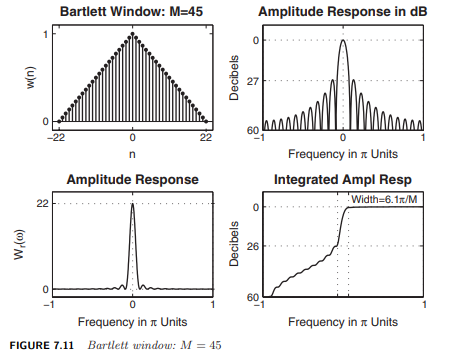
\includegraphics[width=1\linewidth]{Bartlett.png}
    \label{fig:enter-label}
\end{figure}
\subsubsection{Hann Window \& Hamming Window}
Hann Window
\begin{equation}
w(n) = \begin{cases}
0.5[1-\cos(\frac{2\pi n}{M-1})], & 0 \leq n \leq M - 1 \\
0, & \text{otherwise}
\end{cases}
\end{equation}
Hamming Window
\begin{equation}
w(n) = \begin{cases}
0.54-0.46\cos(\frac{2\pi n}{M-1}), 0 \leq n \leq M -1 \\
0, & \text{otherwise}
\end{cases}
\end{equation}
\begin{figure}[H]
    \centering
    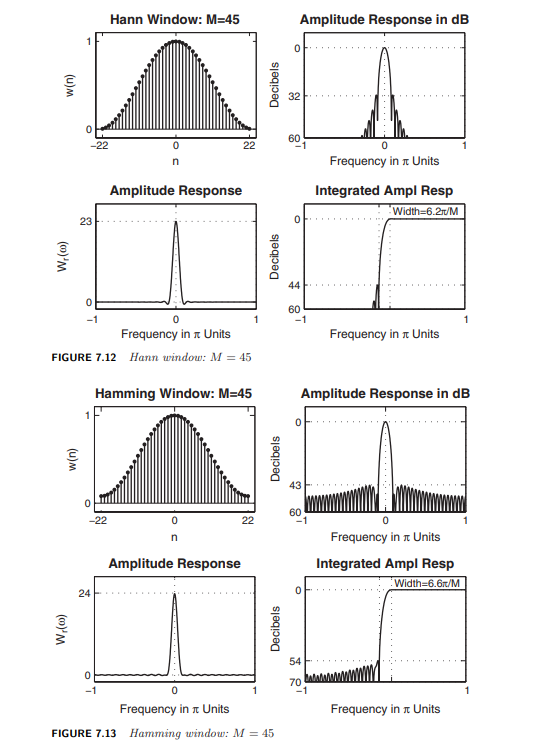
\includegraphics[width=1\linewidth]{HannHamming.png}
    \label{fig:enter-label}
\end{figure}
\subsubsection{Blackman Window}
\begin{equation}
w(n) = \begin{cases}
0.42-0.5\cos(\frac{2\pi n}{M-1})+0.08\cos(\frac{4\pi n}{M-1}), 0 \leq n \leq M -1 \\
0, &\text{otherwise}
\end{cases}
\end{equation}
\begin{figure}[H]
    \centering
    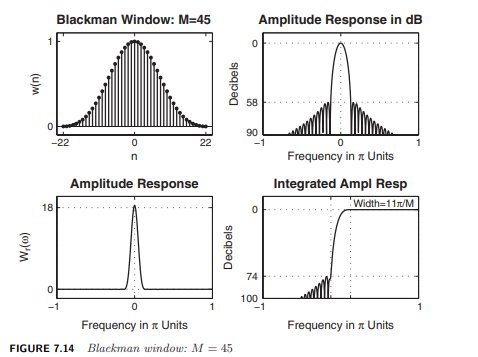
\includegraphics[width=1\linewidth]{Blackman.png}
    \label{fig:enter-label}
\end{figure}
\subsubsection{Kaiser Window}
This is an adjustable window function that is widely used in practice. The
window function is due to J.F. Kaiser and is given by
\begin{equation}
w(n) = \frac{I_0[\beta\sqrt{1-(1-\frac{2n}{M-1})^2}]}{I_0[\beta]}, 0 \leq n \leq M-1
\end{equation}
$I_0[*]$ is the modified zero-order Bessel function given by
\begin{equation}
I_0(x)= 1 + \sum_{k=0}^{\infty}[\frac{(x/2)^{k}}{k!}]^2
\end{equation}
• If $\beta$ = 5.658, then the transition width is equal to 7.8$\pi$/M, and the
minimum stopband attenuation is equal to 60 dB. This is shown in
Figure 7.15. \\
• If $\beta$ = 4.538, then the transition width is equal to 5.8$\pi$/M, and the
minimum stopband attenuation is equal to 50 dB. \\
\vspace{1em}
Given $w_p, w_s, R_p, A_s$, the parameters M and $\beta$ are given by. \\
\begin{equation}
\text{Transition bandwith} = \Delta w = w_s-w_p
\end{equation}
\begin{equation}
\text{Filter length M =} \frac{A_s-7.95}{2.285\Delta w+1 }
\end{equation}

\begin{figure}[H]
    \centering
    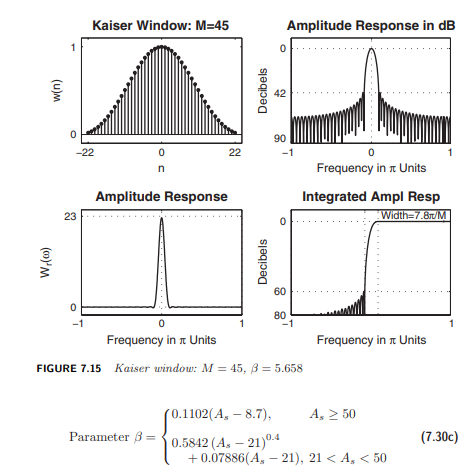
\includegraphics[width=1\linewidth]{KaiserWindow.png}
\end{figure}

\newpage
\subsubsection{MATLAB implementation}
MATLAB provides several functions to implement window functions discussed in this section. A brief description of these functions follow.
• w=boxcar(M) returns the M-point rectangular window function in
array w.
• w=bartlett(M) returns the M-point Bartlett window function in
array w. \\
• w=hann(M) returns the M-point Hann window function in array w.\\
• w=hamming(M) returns the M-point Hamming window function in
array w. \\
• w=blackman(M) returns the M-point Blackman window function in
array w. \\
• w=kaiser(M,beta) returns the beta-valued M-point rectangular
window function in array w. \\
\vspace{1em}
The below function does ideal lowpass filter computation
\begin{lstlisting}
function hd = ideal_lp(wc,M);
% Ideal lowpass filter computation
% --------------------------------
% [hd] = ideal_lp(wc,M)
% hd = ideal impulse response between 0 to M-1
% wc = cutoff frequency in radians
% M = length of the ideal filter
%
alpha = (M-1)/2; n = [0:1:(M-1)];
m=n- alpha; fc = wc/pi; hd = fc*sinc(fc*m);
\end{lstlisting}
To display the frequency-domain plots of digital filters, MATLAB
provides the freqz function, which we used in earlier chapters. Using this
function, we have developed a modified version, called freqz m, which
returns the magnitude response in absolute as well as in relative dB scale,
the phase response, and the group delay response.
\begin{lstlisting}
function [db,mag,pha,grd,w] = freqz_m(b,a);
% Modified version of freqz subroutine
% ------------------------------------
% [db,mag,pha,grd,w] = freqz_m(b,a);
% db = relative magnitude in dB computed over 0 to pi radians
% mag = absolute magnitude computed over 0 to pi radians
% pha = phase response in radians over 0 to pi radians
% grd = group delay over 0 to pi radians
% w = 501 frequency samples between 0 to pi radians
% b = numerator polynomial of H(z) (for FIR: b=h)
% a = denominator polynomial of H(z) (for FIR: a=[1])
%
[H,w] = freqz(b,a,1000,'whole');
H = (H(1:1:501))'; w = (w(1:1:501))';
mag = abs(H); db = 20*log10((mag+eps)/max(mag));
pha = angle(H); grd = grpdelay(b,a,w);    
\end{lstlisting}
Design a digital FIR lowpass filter with the following specifications:
\vspace{1em}
Passband cutoff: $w_p=0.2\pi$; Passband ripple: $R_p=0.25$ dB \\
\vspace{1em}
Stopband cutoff: $w_s=0.3\pi$; Stopband ripple: $A_s =50$ dB \\
\vspace{1em}
Choose an appropriate window function from Table 7.1. Determine the impulse
response and provide a plot of the frequency response of the designed filter
\begin{lstlisting}
 wp = 0.2*pi; ws = 0.3*pi; tr_width = ws - wp;
 M = ceil(6.6*pi/tr_width) + 1
M = 67
 n=[0:1:M-1];
 wc = (ws+wp)/2, % Ideal LPF cutoff frequency
 hd = ideal_lp(wc,M); w_ham = (hamming(M))'; h = hd .* w_ham;
 [db,mag,pha,grd,w] = freqz_m(h,[1]); delta_w = 2*pi/1000;
 Rp = -(min(db(1:1:wp/delta_w+1))); % Actual passband ripple
Rp = 0.0394
 As = -round(max(db(ws/delta_w+1:1:501))) % Min stopband attenuation
As = 52
% plotting commands follow    
\end{lstlisting}
For the design specifications given in the above example, choose the Kaiser window
to design the necessary lowpass filter
\begin{lstlisting}
 wp = 0.2*pi; ws = 0.3*pi; As = 50; tr_width = ws - wp;
 M = ceil((As-7.95)/(2.285*tr_width)+1) + 1
M = 61
 n=[0:1:M-1]; beta = 0.1102*(As-8.7)
beta = 4.5513
 wc = (ws+wp)/2; hd = ideal_lp(wc,M);
 w_kai = (kaiser(M,beta))'; h = hd .* w_kai;
 [db,mag,pha,grd,w] = freqz_m(h,[1]); delta_w = 2*pi/1000;
 As = -round(max(db(ws/delta_w+1:1:501))) % Min stopband attenuation
As = 52
% plotting commands follow    
\end{lstlisting}
\begin{figure}[H]
    \centering
    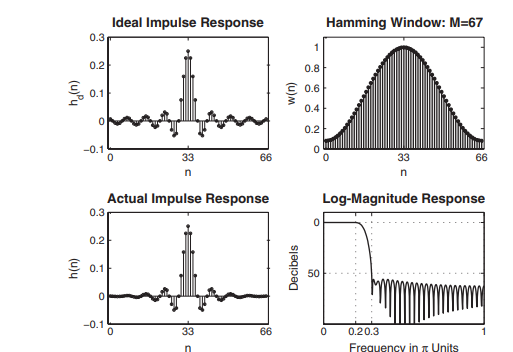
\includegraphics[width=0.75\linewidth]{7.8MATLAB.png}
\end{figure}
\newpage
Let us design the following digital bandpass filter.
\begin{center}
lower stopband edge: $\omega_{1s}= 0.2\pi, A_s=$60dB \\
lower stopband edge: $\omega_{1p}= 0.35\pi, R_p=$1dB \\
lower stopband edge: $\omega_{2p}= 0.65\pi, R_p =$1dB \\
lower stopband edge: $\omega_{2s}= 0.8\pi, A_s=$60 dB \\
\end{center}
\begin{figure}[H]
    \centering
    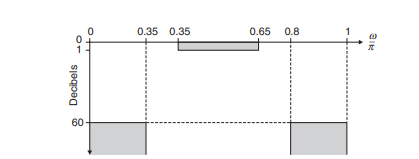
\includegraphics[width=0.75\linewidth]{FIRBandSpecs.png}
\end{figure}
\begin{lstlisting}
 ws1 = 0.2*pi; wp1 = 0.35*pi; wp2 = 0.65*pi; ws2 = 0.8*pi; As = 60;
 tr_width = min((wp1-ws1),(ws2-wp2)); M = ceil(11*pi/tr_width) + 1
M = 75
 n=[0:1:M-1]; wc1 = (ws1+wp1)/2; wc2 = (wp2+ws2)/2;
 hd = ideal_lp(wc2,M) - ideal_lp(wc1,M);
 w_bla = (blackman(M))'; h = hd .* w_bla;
 [db,mag,pha,grd,w] = freqz_m(h,[1]); delta_w = 2*pi/1000;
 Rp = -min(db(wp1/delta_w+1:1:wp2/delta_w)) % Actual passband ripple
Rp = 0.0030
 As = -round(max(db(ws2/delta_w+1:1:501))) % Min stopband attenuation
As = 75
% plotting commands follow    
\end{lstlisting}
\begin{figure}[H]
    \centering
    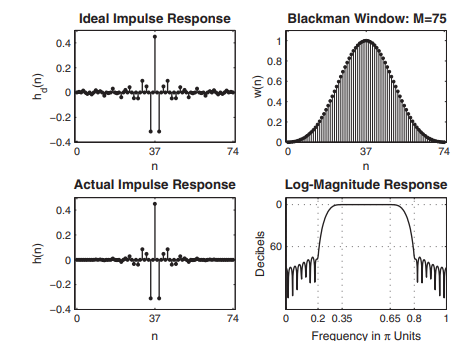
\includegraphics[width=0.75\linewidth]{BlackManBandPass.png}
\end{figure}
The frequency response of an ideal bandstop filter is given by
\begin{center}
$H_e(e^{jw})=\begin{cases}
1, & 0 \leq |\omega| < \pi/3 \\
0, & \pi/3 \leq |\omega| \leq 2\pi/3 \\
1, & 2\pi/3 < |\omega| \leq \pi
\end{cases}$
\end{center}
Using a Kaiser window, design a bandstop filter of length 45 with stopband
attenuation of 60 dB.
\vspace{1em}
$\beta= 0.1102*(A_s-8.7)$
\begin{lstlisting}
 M = 45; As = 60; n=[0:1:M-1];
 beta = 0.1102*(As-8.7)
beta = 5.6533
 w_kai = (kaiser(M,beta))'; wc1 = pi/3; wc2 = 2*pi/3;
 hd = ideal_lp(wc1,M) + ideal_lp(pi,M) - ideal_lp(wc2,M);
 h = hd .* w_kai; [db,mag,pha,grd,w] = freqz_m(h,[1]);
 plotting commands follow
\end{lstlisting}
\begin{figure}[H]
    \centering
    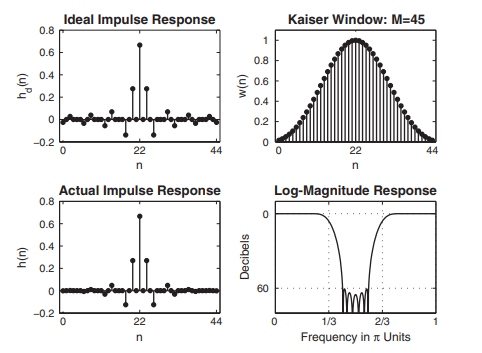
\includegraphics[width=0.75\linewidth]{BandStopFIR.png}
\end{figure}
The frequency response of an ideal digital differentiator is given by
\begin{equation}
H_d(e^{jw})=\begin{cases}
jw, & 0 < \omega\leq \pi \\
-jw, & -\pi < \omega < 0
\end{cases}
\end{equation}
Using a Hamming window of length 21, design a digital FIR differentiator. Plot
the time- and the frequency-domain responses.
\vspace{1em}
\begin{center}
$h_d(n) = \fourier[H_d(e^{jw})e^{-j\alpha w}] = $$\begin{cases}
\frac{\cos \pi (n-\alpha)}{(n-\alpha)},n \neq \alpha \\
0, n =\alpha
\end{cases}$
\begin{lstlisting}
 M = 21; alpha = (M-1)/2; n = 0:M-1;
 hd = (cos(pi*(n-alpha)))./(n-alpha); hd(alpha+1)=0;
 w_ham = (hamming(M))'; h = hd .* w_ham; [Hr,w,P,L] = Hr_Type3(h);
% plotting commands follow    
\end{lstlisting}
\end{center}
\begin{figure}[H]
    \centering
    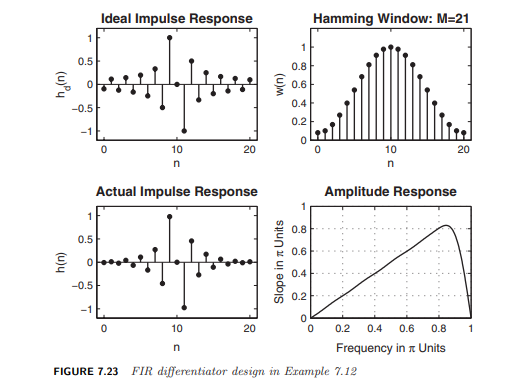
\includegraphics[width=1\linewidth]{FIRDifferentiatior.png}
\end{figure}
\newpage
Design a length-25 digital Hilbert transformer using a Hann window.
\begin{equation}
H_d(e^{jw})=\begin{cases}
-jwe^{-j\alpha w}, & 0 < \omega\leq \pi \\
+jw^{-j\alpha w}, & -\pi < \omega < 0
\end{cases}
\end{equation}
After inverse transformation, the ideal impulse response is given by
\begin{center}
$h_d(n)=$$\begin{cases}
\frac{2}{\pi}\frac{\sin^{2}\pi(n-\alpha)/2}{n-\alpha}, n \neq \alpha \\
0, n = \alpha
\end{cases}$
\begin{lstlisting}
 M = 25; alpha = (M-1)/2; n = 0:M-1;
 hd = (2/pi)*((sin((pi/2)*(n-alpha)).^2)./(n-alpha)); hd(alpha+1)=0;
 w_han = (hann(M))'; h = hd .* w_han; [Hr,w,P,L] = Hr_Type3(h);
 plotting commands follow
\end{lstlisting}
\begin{figure}[H]
    \centering
    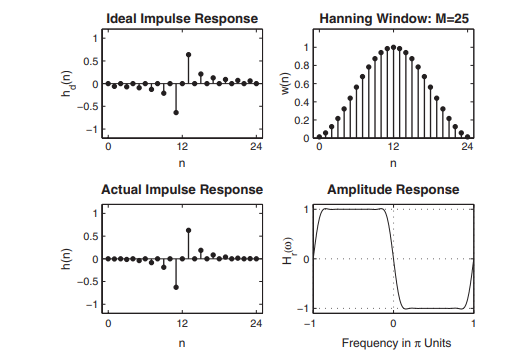
\includegraphics[width=1\linewidth]{HilbertTransformerDesign.png}
\end{figure}
\end{center}
\subsubsection{MATLAB functions}
wc = [wc1 wc2], then fir1 returns a bandpass filter with passband
cutoffs wc1 and wc2. If wc is a multi-element (more than two) vector,
then fir1 returns a multiband filter with cutoffs given in wc. 
\vspace{1em}
• h = fir1(N,wc,'ftype') specifies a filter type, where 'ftype' is:
a. 'high' for a highpass filter with cutoff frequency Wn. \\
b. 'stop' for a bandstop filter, if Wc = [wc1 wc2]. The stopband frequency range is specified by this interval. \\
c. 'DC-1' to make the first band of a multiband filter a passband. \\
d. 'DC-0' to make the first band of a multiband filter a stopband. \\
\vspace{1em}
• h = fir1(N,wc,'ftype',window) or h = fir1(N,wc,window) uses
the vector window of length N+1 obtained from one of the specified
MATLAB window functions. The default window function used is the
Hamming window. \\
\vspace{1em}
To design FIR filters using the Kaiser window, the SP toolbox provides the function kaiserord, which estimates window parameters that
can be used in the fir1 function. The basic syntax is
[N,wc,beta,ftype] = kaiserord(f,m,ripple);

\begin{figure}[H]
    \centering
    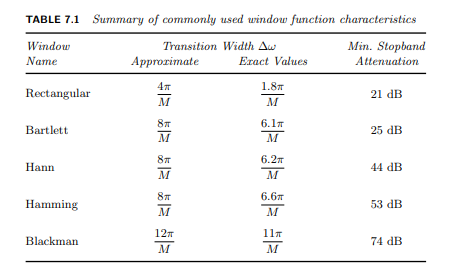
\includegraphics[width=1\linewidth]{WindowFunctionCharacteristics.png}
\end{figure}

\subsection{Frequency-Sampling Technique}
In this design approach, we use the fact that the system function H (z)
can be obtained from the samples H(k) of the frequency response $H(e^{jw}).$ Furthermore, this design technique fits nicely with the frequency-sampling
structure that we discussed in Chapter 6. Let h(n) be the impulse response
of an M-point FIR filter, let H(k) be its M-point DFT, and let H(z) be
its system function
\begin{equation}
H(z) = \sum_{n=0}^{M-1}h(n)z^{-n}=\frac{1-z^{-M}}{M}\sum_{k=0}^{M-1}\frac{H(k)}{1-z^{-1}e^{j2\pi k/M}}
\end{equation}
\begin{equation}
H(e^{jw})=\frac{1-e^{-jwM}}{M}\sum_{k=0}^{M-1}\frac{H(k)}{1-e^{-jw}e^{j2\pi k/M}}
\end{equation}
\begin{equation}
H(k) = H_r(\frac{2\pi k}{M})e^{j\angle H(k)}
\end{equation}
\begin{figure}[H]
    \centering
    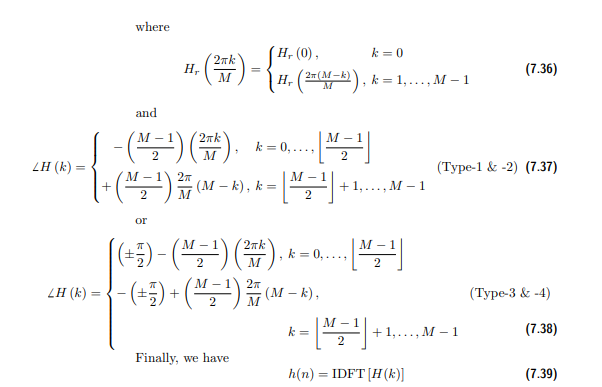
\includegraphics[width=1\linewidth]{ComplexEquations.png}

\end{figure}
\newpage
Given an ideal filter $H_d(e^{jw})$, choose the filter length M
and then sample $H_d(e^{jw})$ at M equispaced frequencies between 0 and
2$\pi$. The actual response $H(e^{jw})$ is the interpolation of the samples H(k)
given by (7.34). This is shown in Figure 7.25. The impulse response is
given by (7.39). Similar steps apply to other frequency-selective filters.
Furthermore, this idea can also be extended for approximating arbitrary
frequency-domain specifications. \\
\vspace{1em}
1. The approximation error—that is, the difference between the ideal and
the actual response—is zero at the sampled frequencies.
2. The approximation error at all other frequencies depends on the shape
of the ideal response; that is, the sharper the ideal response, the larger
the approximation error.
3. The error is larger near the band edges and smaller within the band.
There are two design approaches. In the first approach, we use the
basic idea literally and provide no constraints on the approximation error;
\begin{figure}[H]
    \centering
    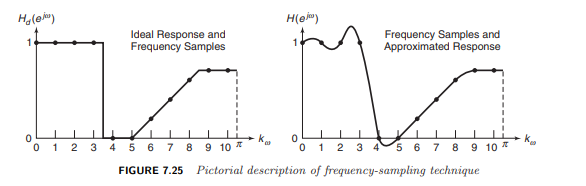
\includegraphics[width=0.75\linewidth]{PictoralDescription.png}
\end{figure}
Consider the lowpass filter specifications from the first example in the MATLAB implementation section of Window design:
\vspace{1em} \\
Passband cutoff: $w_p=0.2\pi$; Passband ripple: $R_p=1$ dB \\
\vspace{1em}
Stopband cutoff: $w_s=0.3\pi$; Stopband ripple: $A_s =16$ dB \\
\vspace{1em}
Let us choose M = 20 so that we have a frequency sample at wp, that is, at
k = 2,
\begin{center}
    $w_p=0.2\pi=\frac{2\pi}{20}2$
\end{center}
and the next sample at ws, that is, at k = 3, 
\begin{center}
    $w_s = 0.3\pi = \frac{2\pi}{20}3$
\end{center}
Thus we have three samples in the passband and seven samples in
the stopband. \\
\vspace{1em}
$H(w) = \underbrace{1,\ldots,1}_{\text{3 ones}},\underbrace{0,\ldots,0}_{\text{13 zeroes}},\underbrace{1,\ldots,1}_{\text{4 ones}}$
\begin{lstlisting}
 M = 20; alpha = (M-1)/2; l = 0:M-1; wl = (2*pi/M)*l;
 Hrs = [1,1,1,zeros(1,15),1,1]; %Ideal amp res sampled
 Hdr = [1,1,0,0]; wdl = [0,0.25,0.25,1]; %Ideal amp res for plotting
 k1 = 0:floor((M-1)/2); k2 = floor((M-1)/2)+1:M-1;
 angH = [-alpha*(2*pi)/M*k1, alpha*(2*pi)/M*(M-k2)];
 H = Hrs.*exp(j*angH); h = real(ifft(H,M));
 [db,mag,pha,grd,w] = freqz_m(h,1); [Hr,ww,a,L] = Hr_Type2(h);
 plotting commands follow
\end{lstlisting}
\begin{figure}[H]
    \centering
    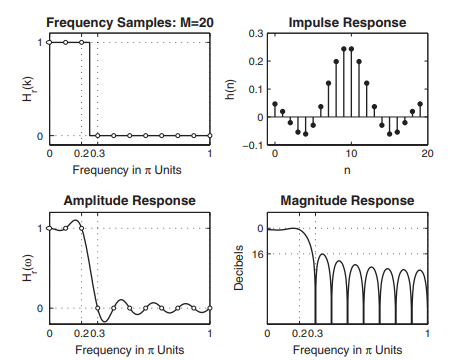
\includegraphics[width=1\linewidth]{NativeDesign.png}
\end{figure}
\subsubsection{Optimum Design Method}
To obtain more attenuation, we will have to increase M and make
the transition band samples free samples—that is, we vary their values
to obtain the largest attenuation for the given M and the transition
width. \\
\vspace{1em}
Using the optimum design method, design a better lowpass filter from previous example: \\
\vspace{1em}
Let us choose M = 40 so that we have one sample in the transition band
$0.2\pi < w < 0.3\pi$. Since $w_1 = \frac{2\pi}{40}$, the transition band samples are at k = 5 and at k = 40 - 5 = 35. Let us denote the value of these samples by $T_1$, $0 < T_1 < 1$. \\
$H(w) = \underbrace{1,\ldots,1}_{\text{5 ones}},T1,\underbrace{0,\ldots,0}_{\text{29 zeroes}},T1,\underbrace{1,\ldots,1}_{\text{6 ones}}$
\begin{lstlisting}
% T1 = 0.5
 M = 40; alpha = (M-1)/2;
 Hrs = [ones(1,5),0.5,zeros(1,29),0.5,ones(1,4)];
 k1 = 0:floor((M-1)/2); k2 = floor((M-1)/2)+1:M-1;
 angH = [-alpha*(2*pi)/M*k1, alpha*(2*pi)/M*(M-k2)];
 H = Hrs.*exp(j*angH);
 h = real(ifft(H,M));
\end{lstlisting}
\begin{figure}[H]
    \centering
    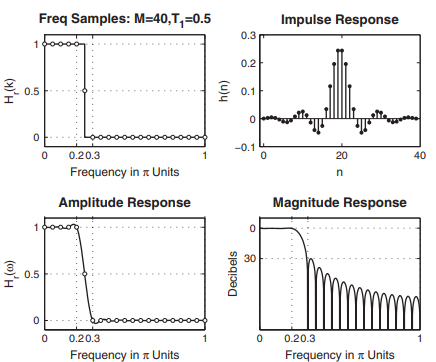
\includegraphics[width=1\linewidth]{Optimum1.png}
\end{figure}
From the plots of this design in, we observe that the minimum
stopband attenuation is now 30 dB, which is better than the naive design attenuation but is still not at the acceptable level of 50 dB. The best value for T1 was obtained by varying it manually. The resulting filter is obtained using the following MATLAB script.
\begin{lstlisting}
% T1 = 0.39
 M = 40; alpha = (M-1)/2;
 Hrs = [ones(1,5),0.39,zeros(1,29),0.39,ones(1,4)];
 k1 = 0:floor((M-1)/2); k2 = floor((M-1)/2)+1:M-1;
 angH = [-alpha*(2*pi)/M*k1, alpha*(2*pi)/M*(M-k2)];
 H = Hrs.*exp(j*angH); h = real(ifft(H,M));
\end{lstlisting}
\begin{figure}[H]
    \centering
    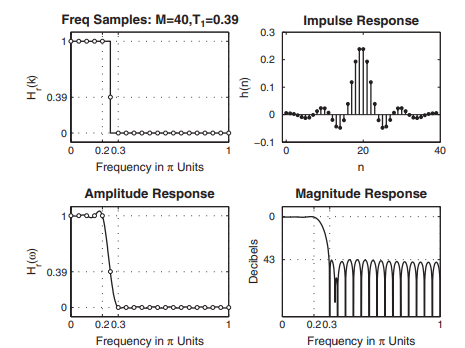
\includegraphics[width=1\linewidth]{Optimum2.png}
\end{figure}
Design the following bandpass filter: \\
\vspace{1em}
Lower stopband edge: $w_s=0.2\pi$, Upper stopband edge: $w_{2_{s}} = 0.8\pi$; Passband ripple: $A_s=60$ dB \\
\vspace{1em}
Lower passband edge: $w_p=0.36\pi$, Upper passband edge: $0.65\pi$; Stopband ripple: $R_p =1$ dB \\
\vspace{1em}
\begin{lstlisting}
 M = 40; alpha = (M-1)/2; l = 0:M-1; wl = (2*pi/M)*l;
 T1 = 0.109021; T2 = 0.59417456;
 Hrs=[zeros(1,5),T1,T2,ones(1,7),T2,T1,zeros(1,9),T1,T2,ones(1,7),T2,T1,zeros(1,4)];
 Hdr = [0,0,1,1,0,0]; wdl = [0,0.2,0.35,0.65,0.8,1];
 k1 = 0:floor((M-1)/2); k2 = floor((M-1)/2)+1:M-1;
 angH = [-alpha*(2*pi)/M*k1, alpha*(2*pi)/M*(M-k2)];
 H = Hrs.*exp(j*angH); h = real(ifft(H,M));
 [db,mag,pha,grd,w] = freqz_m(h,1); [Hr,ww,a,L] = Hr_Type2(h);
\end{lstlisting}
\begin{figure}[H]
    \centering
    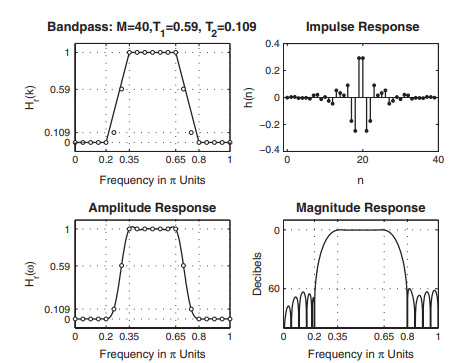
\includegraphics[width=1\linewidth]{BandPassOptimal.png}
\end{figure}
Design the following highpass filter: \\
\vspace{1em}
Stopband edge: $w_s=0.6\pi$; Passband ripple: $A_s=50$ dB \\
\vspace{1em}
Passband edge: $w_p=0.8\pi$; Stopband ripple: $R_p =1$ dB \\
\vspace{1em}
\begin{lstlisting}
 M = 33; alpha = (M-1)/2; l = 0:M-1; wl = (2*pi/M)*l;
 T1 = 0.1095; T2 = 0.598;
 Hrs = [zeros(1,11),T1,T2,ones(1,8),T2,T1,zeros(1,10)];
 Hdr = [0,0,1,1]; wdl = [0,0.6,0.8,1];
 k1 = 0:floor((M-1)/2); k2 = floor((M-1)/2)+1:M-1;
 angH = [-alpha*(2*pi)/M*k1, alpha*(2*pi)/M*(M-k2)];
 H = Hrs.*exp(j*angH); h = real(ifft(H,M));
 [db,mag,pha,grd,w] = freqz_m(h,1); [Hr,ww,a,L] = Hr_Type1(h);    
\end{lstlisting}
\subsubsection{MATLAB functions}
The SP toolbox provides a function called fir2, which combines
the frequency-sampling technique with the window technique to design
arbitrary-shaped magnitude response FIR filters. After computing the filter impulse response using the naive design method, fir2 then applies a
selected window to minimize ripples near the band-edge frequencies. This
function's syntax also has several forms, including: \\
\vspace{1em}
• h = fir2(N,f,m) designs an Nth-order (N = M-1) lowpass FIR filter
and returns the impulse response in vector h. The desired magnitude \\
\vspace{1em}
h = fir2(N,f,m,window) uses the vector window of length N+1 obtained from one of the specified MATLAB window functions. The default window function used is the Hamming window. \\
\vspace{1em}
h = fir2(N,f,m,npt) or h = fir2(N,f,m,npt,window) specifies the
number of points npt for the grid onto which fir2 interpolates the
frequency response. The default npt value is 512. The type of frequency-sampling filter that we considered is called a
Type-A filter, in which the sampled frequencies are \\
\begin{center}
$w_k = \frac{2\pi}{M}k, 0 \leq k \leq M -1$
\end{center}
There is a second set of uniformly spaced samples given by
\begin{center}
$w_k = \frac{2\pi(k+\frac{1}{2})}{M}, 0 \leq k \leq M - 1$
\end{center}
This is called a Type-B filter, for which a frequency-sampling structure is
also available. The expressions for the magnitude response $H(e^{jw})$ and the
impulse response h(n) are somewhat more complicated.
\vspace{1em}
Note that the fir2 does not implement the classic optimum frequencysampling method. By incorporating window design, fir2 has found an
alternative (and somewhat clever) approach to do away with the optimum
transition band values and the associated tables
\subsection{Optimal Equiripple Design Technique}
The last two techniques—namely, the window design and the frequency sampling design—were easy to understand and implement. However, they
have some disadvantages. First, we cannot specify the band frequencies
$w_p$ and $w_s$ precisely in the design; that is, we have to accept whatever
values we obtain after the design. Second, we cannot specify both $\delta_1$ and $\delta_2$ ripple factors simultaneously. Either we have $\delta_1=\delta_2$ in the window
design method, or we can optimize only $\delta_2$ in the frequency-sampling
method. Finally, the approximation error—that is, the difference between
the ideal response and the actual response—is not uniformly distributed
over the band intervals. It is higher near the band edges and smaller in
the regions away from band edges. By distributing the error uniformly,
we can obtain a lower-order filter satisfying the same specifications. Fortunately, a technique exists that can eliminate these three problems. This
technique is somewhat difficult to understand and requires a computer
for its implementation. For linear-phase FIR filters, it is possible to derive a set of conditions
for which it can be proved that the design solution is optimal in the sense
of minimizing the maximum approximation error (sometimes called the
minimax or the Chebyshev error). Filters that have this property are called
equiripple filters because the approximation error is uniformly distributed
in both the passband and the stopband.

\begin{figure}[H]
    \centering
    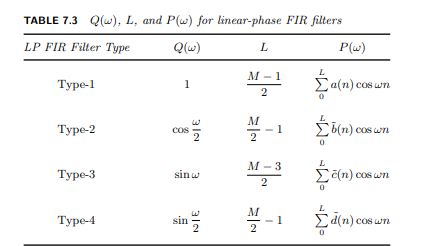
\includegraphics[width=1\linewidth]{QPLFIR.png}
\end{figure}

\subsubsection{Parks–Mccellan Algorithm}
The alternation theorem ensures that the solution to our minimax approximation problem exists and is unique, but it does not tell us how
to obtain this solution. We know neither the order M (or equivalently,
L), nor the extremal frequencies $w_i$, nor the parameters {$\alpha$(n)}, nor the
maximum error $\delta$. Parks and McClellan provided an iterative solution
using the Remez exchange algorithm. It assumes that the filter length M
(or L) and the ratio $\delta_2$/$\delta_1$ are known. If we choose the weighting function
as in (7.43), and if we choose the order M correctly, then $\delta$ = $\delta_2$ when
the solution is obtained. Clearly, $\delta$ and M are related; the larger the M,
the smaller the $\delta$. In the filter specifications, $\delta_1$, $\delta_2$, $\omega_p$, and $\omega_s$ are given. Therefore, M has to be assumed. Fortunately, a simple formula, due to
Kaiser, exists for approximating M. It is given by

\begin{equation}
M = \frac{-20log_{10}\sqrt{\delta_1\delta_2}-13}{2.285\Delta w},\Delta w=w_s-w_p
\end{equation}
\subsubsection{Parks–McClellan in MATLAB}
The function for Parks–McClellan is 
\begin{lstlisting}
[h] = firpm(N,f,m,weights,ftype)  
\end{lstlisting}
There are several version of this syntax:
\textbf{[h] = firpm(N,f,m)} designs an Nth-order (note that the length of the
filter is M = N + 1) FIR digital filter whose frequency response is
specified by the arrays f and m. The filter coefficients (or the impulse
response) are returned in array h of length M. The array f contains
band-edge frequencies in units of $\pi$, that is, 0.$0 \leq f \leq 1$. These frequencies must be in increasing order, starting with 0.0 and ending with
1.0. The array m contains the desired magnitude response at frequencies specified in f. The lengths of f and m arrays must be the same and
must be an even number. The weighting function used in each band is equal to unity, which means that the tolerances ($\delta_i$'s) in every band
are the same. \\
\vspace{1em}
\textbf{[h] = firpm(N,f,m,weights)} is similar to the preceding case except
that the array weights specifies the weighting function in each band.\\
\vspace{1em}
\textbf{[h] = firpm(N,f,m,ftype)} is similar to the first case except that
when ftype is the string ‘differentiator' or ‘hilbert', it designs
digital differentiators or digital Hilbert transformers, respectively. For
the digital Hilbert transformer, the lowest frequency in the f array
should not be 0, and the highest frequency should not be 1. For the
digital differentiator, the m vector does not specify the desired slope in
each band but the desired magnitude. \\
\vspace{1em}
\textbf{[h] = firpm(N,f,m,weights,ftype)} is similar to the above case except that the array weights specifies the weighting function in each
band. \\
\vspace{1em}
To estimate the filter order N, the SP toolbox provides the function
firpmord, which also estimates other parameters that can be used in the
firpm function. The basic syntax is
\begin{lstlisting}
[N,f0,m0,weights] = firpmord(f,m,delta);    
\end{lstlisting}
The function computes the window order N, the normalized frequency
band edges in f0, amplitude response in a0, and the band weights in
weights. The vector f is a vector of normalized band edges and m is a
vector specifying the desired amplitude on the bands defined by f. The
length of f is 2 less than twice the length of m; that is, f does not contain 0
or 1. The vector delta specifies tolerances in each band (not in decibels).
The estimated parameters can now be used in the firpm function.
\vspace{1em}

Design a digital FIR lowpass filter with the following specifications using the Parks–
McClellan algorithm:
\vspace{1em}

Passband cutoff: $w_p=0.2\pi$; Passband ripple: $R_p=0.25$ dB \\
\vspace{1em}
Stopband cutoff: $w_s=0.3\pi$; Stopband ripple: $A_s =50$ dB \\
\vspace{1em}
\begin{lstlisting}
 wp = 0.2*pi; ws = 0.3*pi; Rp = 0.25; As = 50;
 [delta1,delta2] = db2delta(Rp,As);
 [N,f,m,weights] = firpmord([wp,ws]/pi,[1,0],[delta1,delta2]);
 h = firpm(N,f,m,weights);
 [db,mag,pha,grd,w] = freqz_m(h,[1]);
 delta_w = 2*pi/1000; wsi=ws/delta_w+1; wpi = wp/delta_w;
 Asd = -max(db(wsi:1:501))
Asd = 47.8404
 N = N+1
N = 43
 h = firpm(N,f,m,weights); [db,mag,pha,grd,w] = freqz_m(h,[1]);
 Asd = -max(db(wsi:1:501))
Asd = 48.2131
 N = N+1
N = 44
 h = firpm(N,f,m,weights); [db,mag,pha,grd,w] = freqz_m(h,[1]);
 Asd = -max(db(wsi:1:501))
Asd = 48.8689
 N = N+1
N = 45
 h = firpm(N,f,m,weights); [db,mag,pha,grd,w] = freqz_m(h,[1]);
 Asd = -max(db(wsi:1:501))
Asd = 49.8241
 N = N+1
N = 46
 h = firpm(N,f,m,weights); [db,mag,pha,grd,w] = freqz_m(h,[1]);
 Asd = -max(db(wsi:1:501))
Asd = 51.0857
 M = N+1
M = 47
\end{lstlisting}
\begin{figure}[H]
    \centering
    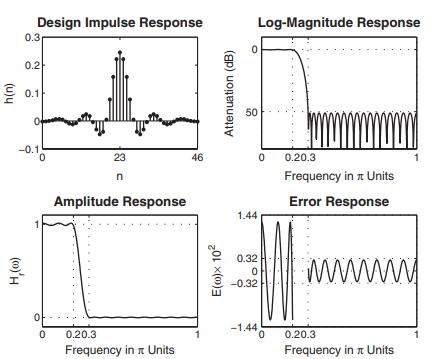
\includegraphics[width=1\linewidth]{Parks1.png}
\end{figure}
Note that we stopped this iterative procedure when the computed stopband
attenuation exceeded the given stopband attenuation As and the optimal
value of M was found to be 47. This value is considerably lower than the
window design techniques (M = 61 for a Kaiser window) or the frequency sampling technique (M = 60). \\
\vspace{1em}
Let us design the following digital bandpass filter using the algorithm.
\begin{center}
lower stopband edge: $\omega_{1s}= 0.2\pi, A_s=$60dB \\
lower passband edge: $\omega_{1p}= 0.35\pi, R_p=$1dB \\
upper passband edge: $\omega_{2p}= 0.65\pi, R_p =$1dB \\
upper stopband edge: $\omega_{2s}= 0.8\pi, A_s=$60 dB \\
\end{center}
\begin{lstlisting}
 ws1 = 0.2*pi; wp1 = 0.35*pi; wp2 = 0.65*pi; ws2 = 0.8*pi;
 Rp = 1.0; As = 60;
 [delta1,delta2] = db2delta(Rp,As);
 f = [ws1,wp1,wp2,ws2]/pi; m = [0,1,0]; delta = [delta2,delta1,delta2];
 [N,f,m,weights] = firpmord(f,m,delta); N
N = 26
 h = firpm(N,f,m,weights);
 [db,mag,pha,grd,w] = freqz_m(h,[1]);
 delta_w=2*pi/1000;
 ws1i=floor(ws1/delta_w)+1; wp1i = floor(wp1/delta_w)+1;
 ws2i=floor(ws2/delta_w)+1; wp2i = floor(wp2/delta_w)+1;
 Asd = -max(db(1:1:ws1i))
Asd = 54.7756
 N = N+1;
 h = firpm(N,f,m,weights);
 [db,mag,pha,grd,w] = freqz_m(h,[1]);
 Asd = -max(db(1:1:ws1i))    
Asd = 56.5910
 N = N+1;
 h = firpm(N,f,m,weights);
 [db,mag,pha,grd,w] = freqz_m(h,[1]);
Asd = -max(db(1:1:ws1i))
 Asd = 61.2843
 M = N+1
M = 29
\end{lstlisting}
\begin{figure}[H]
    \centering
    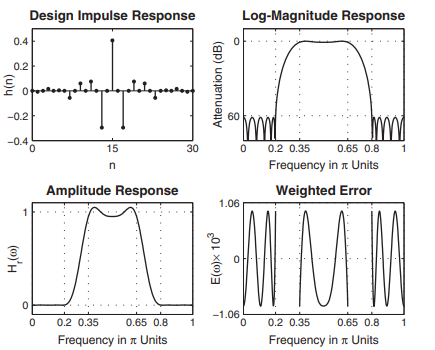
\includegraphics[width=1\linewidth]{Parks2.png}
\end{figure}
Design a highpass filter that has the following specifications:
\begin{center}
$\omega_{s}= 0.6\pi, A_s=$50dB \\
$\omega_{p}= 0.75\pi, R_p=$0.5dB \\
\end{center}
Since this is a highpass filter, we must ensure that the length M is an odd
number. 
\begin{lstlisting}
 ws = 0.6*pi; wp = 0.75*pi; Rp = 0.5; As = 50;
 [delta1,delta2] = db2delta(Rp,As);
 [N,f,m,weights] = firpmord([ws,wp]/pi,[0,1],[delta2,delta1]); N
N = 26
 h = firpm(N,f,m,weights);
 [db,mag,pha,grd,w] = freqz_m(h,[1]);
 delta_w = 2*pi/1000; wsi=ws/delta_w; wpi = wp/delta_w;
 Asd = -max(db(1:1:wsi))
Asd = 49.5918
 N = N+2;
 h = firpm(N,f,m,weights);
 [db,mag,pha,grd,w] = freqz_m(h,[1]);
 Asd = -max(db(1:1:wsi))
 Asd = 50.2253
 M = N+1
M = 29   
\end{lstlisting}
Note also that we increased the value of N by two to maintain its even value.
The optimum M was found to be 29.
\vspace{1em}
Design a "staircase" filter which has 3 bands with different t ideal responses and different tolerances in each band. The design specifications are as follows.
\begin{center}
Band-1: $0 \leq \omega \leq 0.3\pi,$ Ideal gain = 1, Tolerance $\delta_1 = 0.01$ \\
Band-2: $0.4 \leq \omega \leq 0.7\pi,$ Ideal gain = 0.5, Tolerance $\delta_1 = 0.005$ \\
Band-3: $0.8 \leq \omega \leq \pi,$ Ideal gain = 0, Tolerance $\delta_1 = 0.001$ \\
\end{center}
\begin{lstlisting}
 w1 = 0; w2 = 0.3*pi; delta1 = 0.01;
 w3 = 0.4*pi; w4 = 0.7*pi; delta2 = 0.005;
 w5 = 0.8*pi; w6 = pi; delta3 = 0.001;
 weights = [delta3/delta1 delta3/delta2 1];
 Dw = min((w3-w2), (w5-w3));
 M = ceil((-20*log10((delta1*delta2*delta3)^(1/3))-13)/(2.285*Dw)+1)
 M = 51
 f = [0 w2/pi w3/pi w4/pi w5/pi 1];
 m = [1 1 0.5 0.5 0 0];
 h = firpm(M-1,f,m,weights);
 [db,mag,pha,grd,w] = freqz_m(h,[1]);
 delta_w = 2*pi/1000;
 w1i=floor(w1/delta_w)+1; w2i = floor(w2/delta_w)+1;
 w3i=floor(w3/delta_w)+1; w4i = floor(w4/delta_w)+1;
 w5i=floor(w5/delta_w)+1; w6i = floor(w6/delta_w)+1;
 Asd = -max(db(w5i:w6i))
Asd = 62.0745
 M = M-1; h = firpm(M-1,f,m,weights);
 [db,mag,pha,grd,w] = freqz_m(h,[1]);
 Asd = -max(db(w5i:w6i))
Asd = 60.0299
 M = M-1; h = firpm(M-1,f,m,weights);
 [db,mag,pha,grd,w] = freqz_m(h,[1]);
 Asd = -max(db(w5i:w6i))
Asd = 60.6068
 M
M = 49
\end{lstlisting}
\begin{figure}[H]
    \centering
    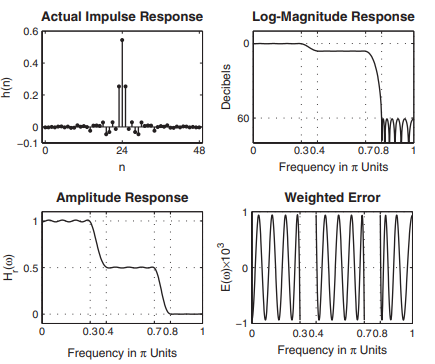
\includegraphics[width=1\linewidth]{Parks3.png}
\end{figure}
In this example, we will design a digital differentiator with different slopes in
each band. The specifications are as follows.
\begin{center}
Band-1: $0 \leq \omega \leq 0.2\pi,$ Slope = 1 sam/cycle = $0.0 \leq |H| \leq 0.1$\\
Band-2: $0.4 \leq \omega \leq 0.6\pi,$ Slope = 2 sam/cycle = $0.4 \leq |H| \leq 0.6$\\
Band-3: $0.8 \leq \omega \leq \pi,$ Slope = 3 sam/cycle = = $1.2 \leq |H| \leq 1.5$\\
\end{center}
The desired magnitude response values in each band can be obtained by multiplying band-edge frequencies in cycles/sam by the slope values
in sam/cycle: \\
\begin{center}
Band-1: $0 \leq f \leq 0.1,$ Slope = 1 sam/cycle = $0.0 \leq |H| \leq 0.1$\\
Band-2: $0.2 \leq f \leq 0.3,$ Slope = 2 sam/cycle = $0.4 \leq |H| \leq 0.6$\\
Band-3: $0.4 \leq f \leq 0.5,$ Slope = 3 sam/cycle = = $1.2 \leq |H| \leq 1.5$\\
\end{center}
\vspace{1em}
Let the weights be equal in all bands. MATLAB script:
\begin{lstlisting}
 f = [0 0.2 0.4 0.6 0.8 1]; % In w/pi units
 m = [0,0.1,0.4,0.6,1.2,1.5]; % Magnitude values
 h = firpm(25,f,m,'differentiator');
 [db,mag,pha,grd,w] = freqz_m(h,[1]);
% Plot commands follow   
\end{lstlisting}
Finally, we design a Hilbert transformer over the band $0.05\pi \leq \omega \leq 0.95\pi$. Since this is a wideband Hilbert transformer, we will choose an odd length for
our filter (i.e., a Type-3 filter). Let us choose M = 51
\begin{lstlisting}
 f = [0.05,0.95]; m = [1 1]; h = firpm(50,f,m,'hilbert');
 [db,mag,pha,grd,w] = freqz_m(h,[1]);
% Plot commands follow
\end{lstlisting}
\begin{figure}[H]
    \centering
    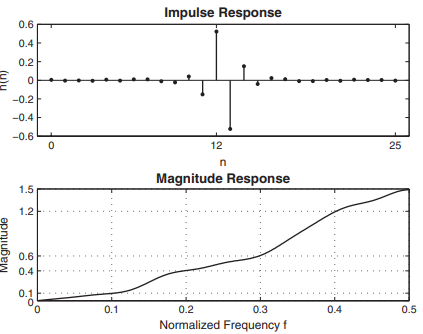
\includegraphics[width=0.75\linewidth]{Differentiator.png}
    \caption{Differentiator Plot}
\end{figure}
\begin{figure}
    \centering
    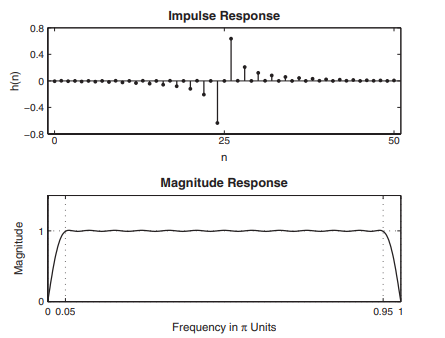
\includegraphics[width=0.75\linewidth]{HilbertTransformer.png}
    \caption{Hilbert Transformer }
\end{figure}
\newpage
\section{IIR Filter Design: The Theory}
IIR filters have infinite-duration impulse responses, hence they can be
matched to analog filters, all of which generally have infinitely long impulse responses. Therefore the basic technique of IIR filter design transforms well-known analog filters into digital filters using complex-valued
mappings. The advantage of this technique lies in the fact that both
analog filter design (AFD) tables and the mappings are available extensively in the literature. This basic technique is called the A/D (analogto-digital) filter transformation. However, the AFD tables are available
only for lowpass filters. We also want to design other frequency-selective
filters (highpass, bandpass, bandstop, etc.). To do this, we need to apply
frequency-band transformations to lowpass filters. These transformations
are also complex-valued mappings, and they are also available in the literature. There are two approaches to this basic technique of IIR filter design: \\
\vspace{1em}
Approach 1: \\
\vspace{1em}
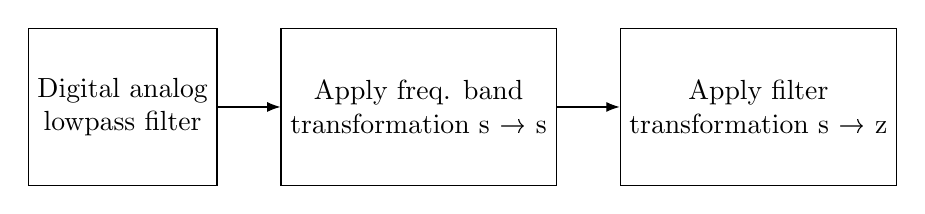
\begin{tikzpicture}[
  node distance=1.8cm and 0.8cm,
  box/.style={draw, minimum width=1.6cm, minimum height=2cm},
  arrow/.style={-Latex}
]
    

% Nodes
\node[box, align=center] (n1) {Digital analog \\lowpass filter};
\node[box, align=center, right=of n1] (n2) {Apply freq. band \\ transformation s → s};
\node[box, align=center, right=of n2] (n3) {Apply filter \\transformation s → z};


% Pointers
\draw[arrow] (n1) -- (n2);
\draw[arrow] (n2) -- (n3);

\end{tikzpicture}

Approach 2: \\
\vspace{1em}

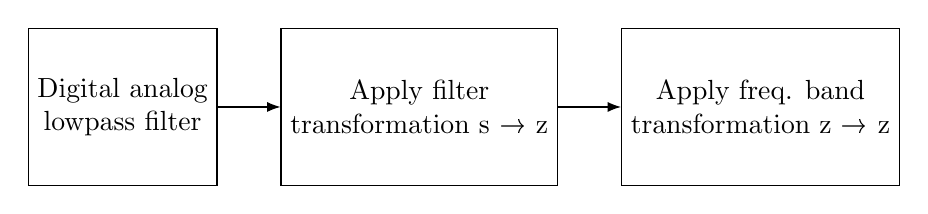
\begin{tikzpicture}[
  node distance=1.8cm and 0.8cm,
  box/.style={draw, minimum width=1.6cm, minimum height=2cm},
  arrow/.style={-Latex}
]
    

% Nodes
\node[box, align=center] (n1) {Digital analog \\lowpass filter};
\node[box, align=center, right=of n1] (n2) {Apply filter \\transformation s → z};
\node[box, align=center, right=of n2] (n3) {Apply freq. band \\ transformation z → z};


% Pointers
\draw[arrow] (n1) -- (n2);
\draw[arrow] (n2) -- (n3);

\end{tikzpicture} \\
\vspace{1em}
The first approach is used in MATLAB to design IIR filters. A
straightforward use of these MATLAB functions does not provide any
insight into the design methodology. Therefore we will study the second
approach because it involves the frequency-band transformation in the
digital domain. 

\newpage
\subsection{Preliminaries}
Let $H_a(jw)$ be the frequency response of an analog filter. Then the lowpass
filter specifications on the magnitude-squared response are given by 

\begin{center}
$$\frac{1}{1+\epsilon^2} \leq |H_a(jw)|^2 \leq 1, $$    $|w| \leq w_p$
$$0 \leq |H_a(jw)|^2 \leq \frac{1}{A^2}, w_s \leq |w|$$
\end{center}
In the above paramaters $\epsilon$ is a passband ripple parameter, $w_p$ is the passband cutoff frequency in rad/sec, A is a stopband attenuation parameter, and $w_s$ is the stopband cutoff in rad/sec.  
\begin{figure}[H]
    \centering
    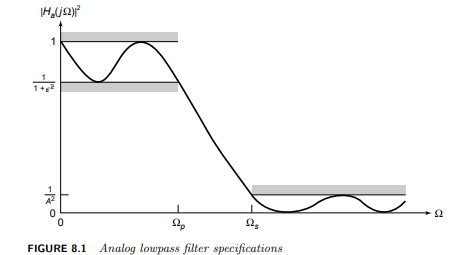
\includegraphics[width=1\linewidth]{Parameters.png}
    \caption{$\Omega = w$}
    \label{fig:enter-label}
\end{figure}
from observation of the above figure, \\
\begin{equation}
|H_a(jw_p)|^2 = \frac{1}{1+\epsilon^2}, w = w_p
\end{equation}
\begin{equation}
|H_a(jw_p)|^2 = \frac{1}{A^2}, w = w_s
\end{equation}
The parameters $\epsilon$ and A are related to $R_p$ and $A_s$, respectively, of the dB scale. These relations are given by
\begin{equation}
R_p = -10log_{10}\frac{1}{1+\epsilon^2} \rightarrow \epsilon =\sqrt{10^{R_p/10} -1}
\end{equation}
and 
\begin{equation}
A_s = -10log_{10}\frac{1}{A^2} \Rightarrow A = 10^{A_s/20}
\end{equation}
\begin{equation}
\epsilon = \frac{2\sqrt{b_1}}{1-\delta_1}, A =\frac{1+\delta_1}{\delta_2}
\end{equation}
\begin{equation}
H_a(s)H(-s)=|H_a(jw)|^2
\end{equation}
\subsection{Filter Types}
\subsubsection{Resonator Filters (Digital Bandpass filters)}
A digital resonator is a special two-pole bandpass filter with a pair of
complex-conjugate poles located very near the unit circle, as shown in
Figure 8.3a. The magnitude of the frequency response of the filter is shown
in Figure 8.3b. The name resonator refers to the fact that the filter has a
large magnitude response in the vicinity of the pole position. The angle of
the pole location determines the resonant frequency of the filter. Digital
resonators are useful in many applications, including simple bandpass
filtering and speech generation. Let us consider the design of a digital resonator with a resonant peak
at or near $w = w_0$. Hence we select the pole position as
\begin{equation}
p_{1,2}= re^{\pm jw_0}
\end{equation}
\begin{figure}[H]
    \centering
    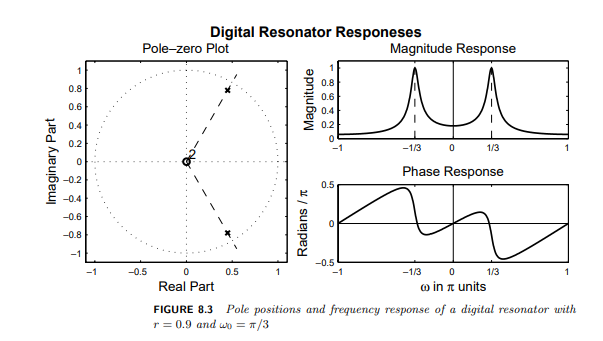
\includegraphics[width=1\linewidth]{Resonator.png}
    \label{fig:enter-label}
\end{figure}
The corresponding transfer function in the z-domain:
\begin{equation}
H(z) = \frac{1}{(1-re^{jw_0}z^{-1})(1-re^{-jw_0}z^{-1})}=\frac{b_0}{1-(2rcosw_{0})z^{-1}+r^2z^{-2}}
\end{equation}
where $b_0$ is a gain parameter. The frequency response is 
\begin{equation}
|H(e^{jw})| = \frac{b_0}{|(1-r)(1-re^{(-jw2_0)})|}= \frac{b_0}{(1-r)\sqrt{1+r^2-2rcos2w_0}}
\end{equation}
The desired gain parameter is 
\begin{equation}
b_0=(1-r)\sqrt{1+r^2-2rcos2w_0}
\end{equation}
The magnitude of the frequency response is
\begin{equation}
|H(e^{jw})|= \frac{b_0}{D_1(w)D_2(w)}
\end{equation}
\begin{center}
$D_1(w)= \sqrt{1+r^2-2rcos(w-w_0)}$ \\
\vspace{1em}
$D_2(w)= \sqrt{1+r^2-2rcos(w+w_0)}$ \\
\vspace{1em}
$w_r = \cos^{-1}(\frac{1+r^2}{2r}\cos w_0)$ \\
\vspace{1em}
$\Delta w = 2(1-r)$
\end{center}
Note: r is the amplitude of oscillation.
\subsubsection{Notch Filters}
A notch filter is a filter that contains one or more deep notches or, ideally, perfect nulls in its frequency response. Figure 8.5 illustrates the frequency response of a notch filter with a null at the frequency $\omega = \omega_0$. Notch filters are useful in many applications where specific frequency components must be eliminated. For example, instrumentation systems require that the power line frequency of 60 Hz and its harmonics be eliminated. To create a null in the frequency response of a filter at a frequency $w_0$, we simply introduce a pair of complex-conjugate zeros on the unit circle at the angle $w_0$. Hence the zeros are selected as 
\begin{equation}
z_{1,2} = e^{\pm jw_0}
\end{equation}
Then the system function for the notch filter is 
\begin{equation}
H(z) = b_0(1- e^{jw_0}z^{-1})(1- e^{-jw_0}z^{-1}) = b_0(1-(2\cos w_0)z^{-1} + z^{-2})
\end{equation}
where $b_0$ is a gain factor. Figure 8.6 illustrates the magnitude response of a notch filter having a null at $\omega = \pi/4$ 
\begin{figure}[H]
    \centering
    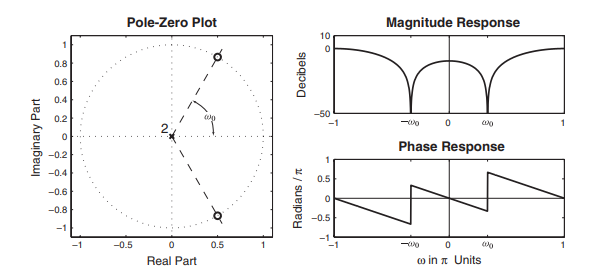
\includegraphics[width=1\linewidth]{NotchIIR.png}
    \caption{Frequency response of a typical notch filter}
    \label{fig:enter-label}
\end{figure}
\begin{figure}[H]
    \centering
    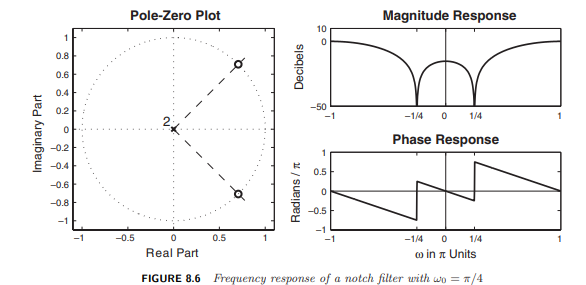
\includegraphics[width=1\linewidth]{Notch1.png}
    \label{fig:enter-label}
\end{figure}
 Alternatively, we could attempt to improve the frequency response of the filter by introducing poles in the system function.
 \begin{figure}
     \centering
     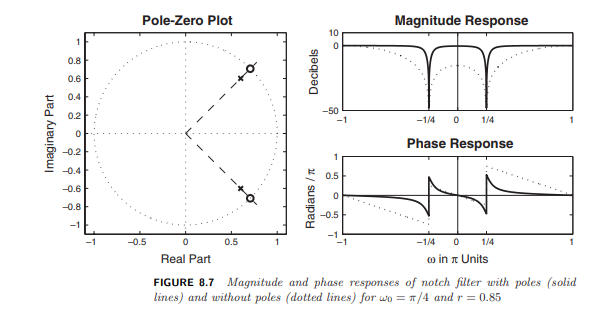
\includegraphics[width=1\linewidth]{Notch2.png}
     \caption{Enter Caption}
     \label{fig:enter-label}
 \end{figure}
In particular, suppose we select the poles at 
\begin{equation}
p_{1,2}=re^{\pm jw_0}
\end{equation}
Hence the system function becomes 
\begin{equation}
H(z) = b_0\frac{1-(2\cos w_0)z^{-1}+z^{-2}}{1-(2r\cos w_0)z^{-1}+r^2z^{-2}}
\end{equation}
\subsubsection{Comb Filters}
In its simplest form, a comb filter may be viewed as a notch filter in which
the nulls occur periodically across the frequency band, hence the analogy
to an ordinary comb that has periodically spaced teeth. Comb filters are
used in many practical systems, including the rejections of power-line
harmonics and the suppression of clutter from fixed objects in moving target indicator (MTI) radars. \\
\vspace{1em}
The frequency response is given as follows
\begin{equation}
H_L(e^{jw})= \sum_{k=0}^{M}h(k)e^{-jkLw}=H(e^{jLw})
\end{equation}
Consequently, the frequency response characteristic $H_L(e^{jw})$ is an L-order repetition of $H(e^{jw})$ in the range $0 \leq \omega \leq 2 \pi $.
\begin{figure}[H]
    \centering
    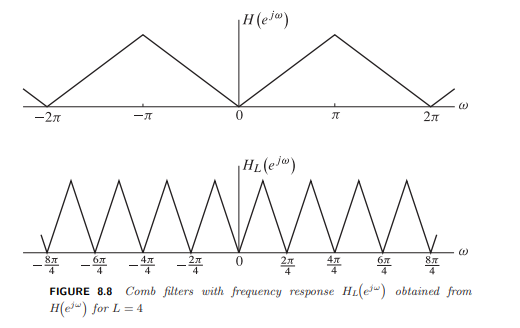
\includegraphics[width=1\linewidth]{Comb.png}
    \label{fig:enter-label}
\end{figure}
By observation, you can see the frequency response repeats 4 times in the span of $2 \pi$ period.
\subsubsection{AllPass Filters}
An allpass filter is characterized by a system function that has a constant
magnitude response for all frequencies, that is,
\begin{equation}
|H(e^{jw})| = 1, 0 \leq \omega \leq \pi
\end{equation}
A simple example of an allpass system is a system that introduces a pure
delay to an input signal, that is,
\begin{equation}
H(z) = z^{-k}
\end{equation}
The general form of an allpass filter:
\begin{equation}
H(z) = \frac{a_N+a_{N-1}+...+a_1z^{-N+1}+z^{-N}}{1+a_1z^{-1}+...+a_{N-1}z^{-N+1}+a_Nz^{-N}}
\end{equation}
alternatively the compact form 
\begin{equation}
H(z) =z^{-N}\frac{A(z^{-1})}{A(z)}, A(z)=\sum_{k=0}^{N}a_kz^{-k},a_0=1
\end{equation}
\begin{figure}[H]
    \centering
    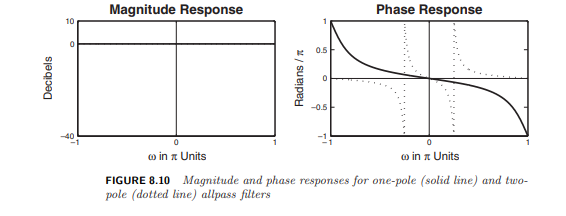
\includegraphics[width=1\linewidth]{Allpass.png}
    \label{fig:enter-label}
\end{figure}
\subsection{Analog Filters}
IIR filter design techniques rely on existing analog filters to obtain digital filters. We designate these analog filters as prototype filters. Three prototypes are widely used in practice. In this section, we briefly summarize the characteristics of the lowpass versions of these prototypes: Butterworth lowpass, Chebyshev lowpass (Type I and II), and Elliptic lowpass.
Although we will use MATLAB functions to design these filters, it is necessary to learn the characteristics of these filters so that we can use proper parameters in MATLAB functions to obtain correct results.
\subsubsection{Butterworth Lowpass}
This filter is characterized by the property that its magnitude response is
flat in both passband and stopband. The magnitude-squared response of
an Nth-order lowpass filter is given by
\begin{equation}
|H_a(jw)|^2=\frac{1}{1+(\frac{w}{w_c})^{2N}}
\end{equation}
N is the order of the filter. Similarly \\
\begin{equation}
H_a(s)=\frac{w_c^N}{\prod_{\textit{LHP Poles}}(s-p_k)}, p_k=w_ce^{j\frac{\pi}{2N}(2k+N+1)}, k=0,1,2N-1
\end{equation}
Meaning that $H_a(s)$ is nothing but the cutoff frequency squared divided by the number of poles in the left plane. 
\begin{figure}[H]
    \centering
    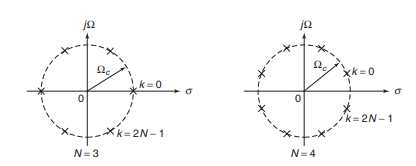
\includegraphics[width=1\linewidth]{Poles.png}
    \label{fig:enter-label}
\end{figure}
Consider $|H_a(jw)|^2=\frac{1}{1+64w^6}=\frac{1}{1+(\frac{w}{0.5})^{2(3)}}$
\begin{center}
$H_a(s)=\frac{1/8}{(s+0.5)(s^2+0.5s+0.25)}$
\end{center}
\subsubsection{Implementation of Butterworth Lowpass}
MATLAB provides a function called [z,p,k]=buttap(N) to design a normalized
d (i.e., wc = 1) Butterworth analog prototype filter of order N, which returns zeros in z array, poles in p array, and the gain value k.
However, we need an unnormalized Butterworth filter with arbitrary wc.
From the example above, we observe that there are no zeros and that the poles
of the unnormalized filter are on a circle with radius wc instead of on a
unit circle. This means that we have to scale the array p of the normalized filter by wc and the gain k by $w_c^N$ . In the following function, called
U\_buttap(N,Omegac), we design the unnormalized Butterworth analog
prototype filter.
\begin{lstlisting}
function [b,a] = u_buttap(N,Omegac);
% Unnormalized Butterworth analog lowpass filter prototype
% --------------------------------------------------------
% [b,a] = u_buttap(N,Omegac);
% b = numerator polynomial coefficients of Ha(s)
% a = denominator polynomial coefficients of Ha(s)
% N = Order of the Butterworth Filter
% Omegac = Cutoff frequency in radians/sec
%
[z,p,k] = buttap(N);
p = p*Omegac;
k = k*Omegac^N;
B = real(poly(z));
b0 = k; b = k*B; a = real(poly(p));    
\end{lstlisting}
This function provides a direct form (or numerator-denominator) structure. Often, we also need a cascade form structure. In Chapter 6, we have
already studied how to convert a direct form into a cascade form. The
following sdir2cas function describes the procedure that is suitable for
analog filters.
\begin{lstlisting}
function [C,B,A] = sdir2cas(b,a);
% DIRECT form to CASCADE form conversion in s-plane
% -------------------------------------------------
% [C,B,A] = sdir2cas(b,a)
% C = gain coefficient
% B = K by 3 matrix of real coefficients containing bk's
% A = K by 3 matrix of real coefficients containing ak's
% b = numerator polynomial coefficients of DIRECT form
% a = denominator polynomial coefficients of DIRECT form
%
Na = length(a)-1; Nb = length(b)-1;
% Compute gain coefficient C
b0 = b(1); b = b/b0; a0 = a(1); a = a/a0; C = b0/a0;
%
% Denominator second-order sections:
p= cplxpair(roots(a)); K = floor(Na/2);
if K*2 == Na % Computation when Na is even
    A = zeros(K,3);
    for n=1:2:Na
        Arow = p(n:1:n+1,:); Arow = poly(Arow);
        A(fix((n+1)/2),:) = real(Arow);
    end
elseif Na == 1 % Computation when Na = 1
    A = [0 real(poly(p))];
else % Computation when Na is odd and > 1
    A = zeros(K+1,3);
    for n=1:2:2*K
        Arow = p(n:1:n+1,:); Arow = poly(Arow);
        A(fix((n+1)/2),:) = real(Arow);
    end
    A(K+1,:) = [0 real(poly(p(Na)))];
end
% Numerator second-order sections:
z = cplxpair(roots(b)); K = floor(Nb/2);
if Nb == 0 % Computation when Nb = 0
    B = [0 0 poly(z)];
elseif K*2 == Nb % Computation when Nb is even
    B = zeros(K,3);
    for n=1:2:Nb
        Brow = z(n:1:n+1,:); Brow = poly(Brow);
        B(fix((n+1)/2),:) = real(Brow);
    end
elseif Nb == 1 % Computation when Nb = 1
    B = [0 real(poly(z))];
else % Computation when Nb is odd and > 1
    B = zeros(K+1,3);
    for n=1:2:2*K
        Brow = z(n:1:n+1,:); Brow = poly(Brow);
        B(fix((n+1)/2),:) = real(Brow);
    end
    B(K+1,:) = [0 real(poly(z(Nb)))];
end
\end{lstlisting}
\newpage
2 Design a third-order Butterworth analog prototype filter with $w_c$ = 0.5 given
\begin{lstlisting}
 N = 3; OmegaC = 0.5; [b,a] = u_buttap(N,OmegaC);
 [C,B,A] = sdir2cas(b,a)
C = 0.1250
B=0 0 1
A = 1.0000 0.5000 0.2500
0 1.0000 0.5000
\end{lstlisting}
\subsubsection{Design Equations Lowpass}
The analog lowpass filter is specified by the parameters $w_p$, $R_p$, $w_s$, and $A_s$. Therefore, the essence of the design in the case of Butterworth filter is to obtain the order N and the cutoff frequency Ωc, given these specifications. We use the following equations
\begin{equation}
N = \frac{log_{10}[(10^\frac{R_p}{10}-1)/(10^\frac{A_s}{10}-1)]}{2log_{10}(w_p/w_s)}
\end{equation}
\begin{equation}
w_c = \frac{w_p}{^{2N}\sqrt{10^{As/10}-1}}
\end{equation}
Alternatively to $w_c$
\begin{equation}
w_c = \frac{w_s}{^{2N}\sqrt{10^{As/10}-1}}
\end{equation}
Design a lowpass Butterworth filter to satisfy the following specifications.
\vspace{1em}
Passband cutoff: $w_p=0.2\pi$; Passband ripple: $R_p=7$dB \\
\vspace{1em}
Stopband cutoff: $w_s= 0.3 \pi$; Stopband ripple: $A_s = 16$dB

\begin{center}
$N = [\frac{log_{10}[(10^{0.7}-1)/(10^{1.6}-1)]}{2log_{10}(0.2\pi/0.3 \pi)}=2.79 \approx 3$ \\
\vspace{1em}
To satisfy the equations at exactly $w_p$ \\
$w_c=\frac{0.2\pi}{^6\sqrt{(10^{0.7}-1)}}=0.4985$ \\
To satisfy the equations at exactly $w_s$ \\
$w_c=\frac{0.3\pi}{^6\sqrt{(10^{1.6}-1)}}=0.5122$
\end{center}
Now we can choose any $w_c$ between the above two numbers. Let us choose $w_c = 0.5$. We have to design a Butterworth filter with N = 3 and $w_c = 0.5$. 
\begin{center}
$H_a(s)=\frac{0.125}{(s+0.5)(s^2+0.5s+0.25)}$ (using pole formula)
\end{center}
Function to design an analog Butterworth lowpass filter, given its specifications.
\begin{lstlisting}
function [b,a] = afd_butt(Wp,Ws,Rp,As);
% Analog lowpass filter design: Butterworth
% -----------------------------------------
% [b,a] = afd_butt(Wp,Ws,Rp,As);
% b = numerator coefficients of Ha(s)
% a = denominator coefficients of Ha(s)
% Wp = passband-edge frequency in rad/sec; Wp > 0
% Ws = stopband-edge frequency in rad/sec; Ws > Wp > 0
% Rp = passband ripple in +dB; (Rp > 0)
% As = stopband attenuation in +dB; (As > 0)
%
if Wp <= 0
    error('Passband edge must be larger than 0')
end
if Ws <= Wp
    error('Stopband edge must be larger than Passband edge')
end
if (Rp <= 0) | (As < 0)
    error('PB ripple and/or SB attenuation must be larger than 0')
end
N = ceil((log10((10^(Rp/10)-1)/(10^(As/10)-1)))/(2*log10(Wp/Ws)));
fprintf('\n*** Butterworth Filter Order = %2.0f \n',N)
OmegaC = Wp/((10^(Rp/10)-1)^(1/(2*N)));
[b,a]=u_buttap(N,OmegaC);    
\end{lstlisting}
To display the frequency-domain plots of analog filters, we provide a
function called freqs m, which is a modified version of a function freqs
provided by MATLAB. This function computes the magnitude response
in absolute as well as in relative dB scale and the phase response
\begin{lstlisting}
function [db,mag,pha,w] = freqs_m(b,a,wmax);
% Computation of s-domain frequency response: Modified version
% ------------------------------------------------------------
% [db,mag,pha,w] = freqs_m(b,a,wmax);
% db = relative magnitude in db over [0 to wmax]
% mag = absolute magnitude over [0 to wmax]
% pha = phase response in radians over [0 to wmax]
% w = array of 500 frequency samples between [0 to wmax]
% b = numerator polynomial coefficents of Ha(s)
% a = denominator polynomial coefficents of Ha(s)
% wmax = maximum frequency in rad/sec over which response is desired
%
w = [0:1:500]*wmax/500; H = freqs(b,a,w);
mag = abs(H); db = 20*log10((mag+eps)/max(mag)); pha = angle(H);    
\end{lstlisting}
The impulse response ha(t) of the analog filter is computed using
MATLAB's impulse function. \\
\vspace{1em}
\newpage
Design the analog Butterworth lowpass filter specified in above example using
MATLAB.
\begin{lstlisting}
 Wp = 0.2*pi; Ws = 0.3*pi; Rp = 7; As = 16;
 Ripple = 10 ^ (-Rp/20); Attn = 10 ^ (-As/20);
 % Analog filter design:
 [b,a] = afd_butt(Wp,Ws,Rp,As);
*** Butterworth Filter Order = 3
 % Calculation of second-order sections:
 [C,B,A] = sdir2cas(b,a)
C = 0.1238
B=0 0 1
A = 1.0000 0.4985 0.2485
0 1.0000 0.4985
 % Calculation of frequency response:
 [db,mag,pha,w] = freqs_m(b,a,0.5*pi);
 % Calculation of impulse response:
 [ha,x,t] = impulse(b,a);    
\end{lstlisting}
The system transfer function is given by 
\begin{center}
$H(s) = \frac{0.1238}{(s^2+0.4985s+0.2485)(s+0.4985)}$
\end{center}
\subsubsection{Chebyshev Lowpass Filters}
There are two types of Chebyshev filters. The Chebyshev-I filters have
equiripple response in the passband, while the Chebyshev-II filters have
equiripple response in the stopband.Recall our discussions regarding equiripple FIR filters. We noted that by choosing a filter that has an equiripple rather than a monotonic behavior, we can obtain a lower-order filter. Therefore, Chebyshev filters provide lower order than Butterworth filters for the same specifications.

\begin{equation}
|H_a(jw)|^2=\frac{1}{1+\epsilon^2{T_N^2}(\frac{w}{w_c})}
\end{equation}
The magnitude-squared response of a Chebyshev-I filter where N is the order of the filter, $\epsilon$ is the passband ripple factor, which is
related to $R_p$, and $T_N(x)$ is the Nth-order Chebyshev polynomial 

\begin{equation}
T_N(x) = \begin{cases}
\cos(N \cos^{-1}(x)) , &  0 \leq x \leq 1 \\
\cosh(\cosh^{-1}(x)), & 1 < x < \infty \\
\end{cases}
\end{equation}
where $x= \frac{\Omega}{\Omega_c}$
\begin{figure}[H]
    \centering
    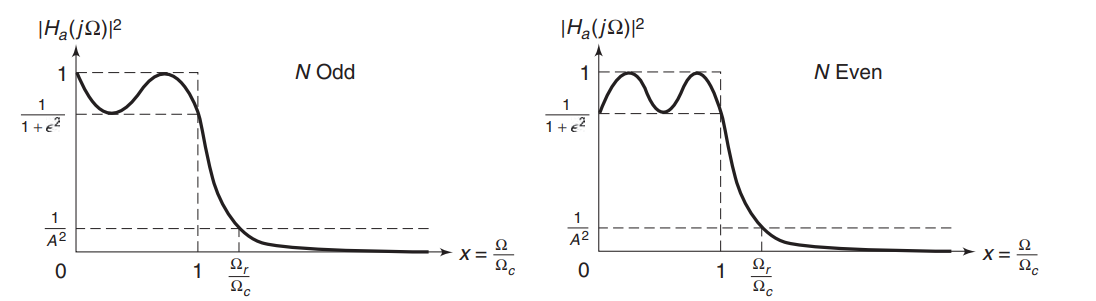
\includegraphics[width=1\linewidth]{Chebyshev.png}
    \label{fig:enter-label}
\end{figure}
Poles of $H_a(s)$
\begin{equation}
p_k = \sigma_k+jw_k, k = 0,...,N-1 
\end{equation}
\begin{equation}
\sigma_k= (a w_c)\cos(\frac{\pi}{2}+\frac{(2k+1)\pi}{2N})
\end{equation}
\begin{equation}
w_k= (bw_c)\sin(\frac{\pi}{2}+\frac{(2k+1)\pi}{2N})
\end{equation}
\begin{equation}
a = \frac{1}{2}(^N\sqrt{\alpha}-{^N\sqrt{1/\alpha}}), b =\frac{1}{2}(^N\sqrt{\alpha}+^N\sqrt{1/\alpha}), \alpha=\frac{1}{\epsilon}+\sqrt{1+\frac{1}{\epsilon^2}}
\end{equation}
The system function is given by 
\begin{equation}
H_a(s)= \frac{K}{\prod_{k}(s-p_k)}
\end{equation}
where $p_k$ are lhp poles and where K is a normalizing factor chosen to make
\begin{equation}
H_a(j0) = \begin{cases}
1 , &  \textit{N odd,} \\
\frac{1}{\sqrt{1+\epsilon^2}}, & \textit{N even,}\\
\end{cases}
\end{equation}
\begin{lstlisting}
function [b,a] = u_chb1ap(N,Rp,Omegac);
% Unnormalized Chebyshev-1 analog lowpass filter prototype
% --------------------------------------------------------
% [b,a] = u_chb1ap(N,Rp,Omegac);
% b = numerator polynomial coefficients
% a = denominator polynomial coefficients
% N = order of the elliptic filter
% Rp = passband ripple in dB; Rp > 0
% Omegac = cutoff frequency in radians/sec
%
[z,p,k] = cheb1ap(N,Rp); a = real(poly(p)); aNn = a(N+1);
p = p*Omegac; a = real(poly(p)); aNu = a(N+1);
k = k*aNu/aNn;
b0 = k; B = real(poly(z)); b = k*B;
\end{lstlisting}
\subsubsection{Design equations}
\begin{equation}
\epsilon = \sqrt{10^{0.1R_p}-1}, A=10^{A_s/20}
\end{equation}
\begin{equation}
w_c=w_p, w_r=\frac{w_s}{w_p}
\end{equation}
\begin{equation}
g = \sqrt{(A^2-1)/\epsilon^2}, N =[\frac{log_{10}[g+\sqrt{g^2-1}]}{log_{10}[w_r+\sqrt{w_r^2-1}]}]
\end{equation}
Design a lowpass Chebyshev-I filter to satisfy the following specifications: \\
\vspace{1em}
Passband cutoff: $w_p=0.2\pi$; Passband ripple: $R_p=1$ dB \\
\vspace{1em}
Stopband cutoff: $w_s=0.3\pi$; Stopband ripple: $A_s =16$ dB \\
\vspace{1em}
\begin{center}
$\epsilon = \sqrt{10^{0.1(1)}-1}=0.5088$, $A=10^{16/20}=6.3096$ \\
\vspace{1em}
$w_c=w_p=0.2\pi, w_r=\frac{0.3\pi}{0.2\pi}=1.5$\\
\vspace{1em}
g =12.2429 (use formula). N = 4 (use formula)
\end{center}
\begin{center}
$\alpha=\frac{1}{\epsilon}+\sqrt{1+\frac{1}{\epsilon^2}} = 4.172$ \\
\vspace{1em}
$b =\frac{1}{2}(^N\sqrt{\alpha}+^N\sqrt{1/\alpha})$ = 1.0644 \\
\vspace{1em}
$a = \frac{1}{2}(^N\sqrt{\alpha}-{^N\sqrt{1/\alpha}}) = 0.3646$ 
\end{center}
Poles:
\begin{center}
$p_k = \sigma_k+jw_k, k = 0,...,N-1 $ \\
\vspace{1em}
$p_{0,3}=  (a w_c)\cos(\frac{\pi}{2}+\frac{(2k+1)\pi}{2N}) +  (bw_c)\sin(\frac{\pi}{2}+\frac{(2k+1)\pi}{2N}) = -0.0877 \pm j0.6179$  \\
\vspace{1em}
$p_{1,2}=  (a w_c)\cos(\frac{\pi}{2}+\frac{(2k+1)\pi}{2N}) +  (bw_c)\sin(\frac{\pi}{2}+\frac{(2k+1)\pi}{2N}) = -0.2117 \pm j0.2559
$
\end{center}
System transfer function:
\begin{center}
$H_a(s)=\frac{0.89125*0.1103*0.3895}{(s^2+0.1754s+0.3895)(s^2+0.4234s+0.1103)}$
\end{center}
Numerator is such that
\begin{center}
$H_a(j0)= \frac{1}{\sqrt{1+\epsilon^2}}=0.89125$
\end{center}
\newpage
\begin{lstlisting}
function [b,a] = afd_chb1(Wp,Ws,Rp,As);
% Analog lowpass filter design: Chebyshev-1
% -----------------------------------------
% [b,a] = afd_chb1(Wp,Ws,Rp,As);
% b = numerator coefficients of Ha(s)
% a = denominator coefficients of Ha(s)
% Wp = passband-edge frequency in rad/sec; Wp > 0
% Ws = stopband-edge frequency in rad/sec; Ws > Wp > 0
% Rp = passband ripple in +dB; (Rp > 0)
% As = stopband attenuation in +dB; (As > 0)
%
if Wp <= 0
    error('Passband edge must be larger than 0')
end
if Ws <= Wp
    error('Stopband edge must be larger than Passband edge')
end
if (Rp <= 0) | (As < 0)
    error('PB ripple and/or SB attenuation must be larger than 0')
end
ep = sqrt(10^(Rp/10)-1); A = 10^(As/20);
OmegaC = Wp; OmegaR = Ws/Wp; g = sqrt(A*A-1)/ep;
N = ceil(log10(g+sqrt(g*g-1))/log10(OmegaR+sqrt(OmegaR*OmegaR-1)));
fprintf('\n*** Chebyshev-1 Filter Order = %2.0f \n',N)
[b,a]=u_chb1ap(N,Rp,OmegaC);
\end{lstlisting}
\begin{lstlisting}
 Wp = 0.2*pi; Ws = 0.3*pi; Rp = 1; As = 16;
 Ripple = 10 ^ (-Rp/20); Attn = 10 ^ (-As/20);
 % Analog filter design:
 [b,a] = afd_chb1(Wp,Ws,Rp,As);
*** Chebyshev-1 Filter Order = 4
 % Calculation of second-order sections:
 [C,B,A] = sdir2cas(b,a)
C = 0.0383
B=0 0 1
A = 1.0000 0.4233 0.1103
1.0000 0.1753 0.3895
 % Calculation of frequency response:
 [db,mag,pha,w] = freqs_m(b,a,0.5*pi);
 % Calculation of impulse response:
 [ha,x,t] = impulse(b,a);
    
\end{lstlisting}
\subsubsection{Chebyshev-II}
A Chebyshev-II filter is related to the Chebyshev-I filter through a
simple transformation. It has a monotone passband and an equiripple
stopband, which implies that this filter has both poles and zeros in the
s-plane. Therefore, the group delay characteristics are better (and the
phase response more linear) in the passband than those of the Chebyshev-I
prototype.
\begin{equation}
|H_a(jw)|^2=\frac{1}{1+[\epsilon^2T_N^2(w_c/w)]^{-1}}
\end{equation}
One approach to designing a Chebyshev-II filter is to design the corresponding Chebyshev-I first and then apply these transformations. The following program provides a function for the design of a Chebyshev-II filter:
\begin{lstlisting}
function [b,a] = afd_chb2(Wp,Ws,Rp,As);
% Analog lowpass filter design: Chebyshev-2
% -----------------------------------------
% [b,a] = afd_chb2(Wp,Ws,Rp,As);
% b = numerator coefficients of Ha(s)
% a = denominator coefficients of Ha(s)
% Wp = passband-edge frequency in rad/sec; Wp > 0
% Ws = stopband-edge frequency in rad/sec; Ws > Wp > 0
% Rp = passband ripple in +dB; (Rp > 0)
% As = stopband attenuation in +dB; (As > 0)
%
if Wp <= 0
    error('Passband edge must be larger than 0')
end
if Ws <= Wp
    error('Stopband edge must be larger than Passband edge')
end
if (Rp <= 0) | (As < 0)
    error('PB ripple and/or SB attenuation must be larger than 0')
end
ep = sqrt(10^(Rp/10)-1); A = 10^(As/20);
OmegaC = Wp; OmegaR = Ws/Wp; g = sqrt(A*A-1)/ep;
N = ceil(log10(g+sqrt(g*g-1))/log10(OmegaR+sqrt(OmegaR*OmegaR-1)));
fprintf('\n*** Chebyshev-2 Filter Order = %2.0f \n',N)
[b,a]=u_chb2ap(N,As,Ws);
\end{lstlisting}
Design a lowpass Chebyshev-II filter to satisfy the following specifications: \\
\vspace{1em}
Passband cutoff: $w_p=0.2\pi$; Passband ripple: $R_p=1$ dB \\
\vspace{1em}
Stopband cutoff: $w_s=0.3\pi$; Stopband ripple: $A_s =16$ dB \\
\vspace{1em}
\begin{lstlisting}
 Wp = 0.2*pi; Ws = 0.3*pi; Rp = 1; As = 16;
 Ripple = 10 ^ (-Rp/20); Attn = 10 ^ (-As/20);
 % Analog filter design:
 [b,a] = afd_chb2(Wp,Ws,Rp,As);
*** Chebyshev-2 Filter Order = 4
 % Calculation of second-order sections:
 [C,B,A] = sdir2cas(b,a)
C = 0.1585
B = 1.0000 0 6.0654
1.0000 0 1.0407
A = 1.0000 1.9521 1.4747
1.0000 0.3719 0.6784
 % Calculation of frequency response:
 [db,mag,pha,w] = freqs_m(b,a,0.5*pi);
 % Calculation of impulse response:
 [ha,x,t] = impulse(b,a);    
\end{lstlisting}
\begin{center}
$H_a(s) =\frac{0.1585(s^2+6.0654)(s^2+1.0407)}{(s^2+1.9521s+1.4747)(s^2+0.3719s+0.6784)}$
\end{center}

\subsubsection{Elliptic Lowpass Filters}
These filters exhibit equiripple behavior in the passband as well as in
the stopband. They are similar in magnitude response characteristics to
the FIR equiripple filters. Therefore, elliptic filters are optimum filters
in that they achieve the minimum order N for the given specifications
(or alternately, achieve the sharpest transition band for the given order
N). These filters, for obvious reasons, are very difficult to analyze and,
therefore, to design. It is not possible to design them using simple tools,
and often programs or tables are needed to design them.

\begin{equation}
|H_a(jw)|^2=\frac{1}{1+\epsilon^2U_N^2(\frac{w}{w_c})}
\end{equation}
where N is the order, $\epsilon$ is the passband ripple, and $U_N$ is the N-th order Jacobian elliptic function.

\begin{equation}
N = \frac{K(k)K({\sqrt{1-k_1^2}})}{K(k_1)K({\sqrt{1-k^2}})}
\end{equation}
\begin{equation}
k = \frac{w_p}{w_s},k_1=\frac{\epsilon}{\sqrt{A^2-1}}
\end{equation}
\begin{equation}
K(x)=\int_0^{\pi/2}\frac{d\theta}{\sqrt{1-x^2\sin^2\theta}}
\end{equation}
is the complete elliptic integral of the first kind. MATLAB provides the
function ellipke to numerically compute the above integral, which we
will use to compute N and to design elliptic filters.
\begin{figure}[H]
    \centering
    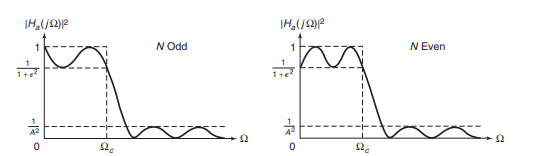
\includegraphics[width=1\linewidth]{Elliptic.png}
    \label{fig:enter-label}
\end{figure}
MATLAB provides a function called [z,p,k]=ellipap(N,Rp,As) to design a normalized elliptic analog prototype filter of order N, passband
ripple Rp, and stopband attenuation As, and that returns zeros in z array,
poles in p array, and the gain value k. We need an unnormalized elliptic
filter with arbitrary wc. This is achieved by scaling the arrays p and z of
the normalized filter by wc and the gain k by the ratio of the unnormalized
to the normalized rational functions evaluated at s = 0. In the following
function, called U elipap(N,Rp,As,Omegac), we design an unnormalized
elliptic analog prototype filter that returns Ha(s) in the direct form.
\begin{lstlisting}
function [b,a] = u_elipap(N,Rp,As,Omegac);
% Unnormalized elliptic analog lowpass filter prototype
% -----------------------------------------------------
% [b,a] = u_elipap(N,Rp,As,Omegac);
% b = numerator polynomial coefficients
% a = denominator polynomial coefficients
% N = order of the elliptic filter
% Rp = passband ripple in dB; Rp > 0
% As = stopband attenuation in dB; As > 0
% Omegac = cutoff frequency in radians/sec
%
[z,p,k] = ellipap(N,Rp,As);
a = real(poly(p)); aNn = a(N+1);
p = p*Omegac; a = real(poly(p)); aNu = a(N+1);
b = real(poly(z)); M = length(b); bNn = b(M);
z = z*Omegac; b = real(poly(z)); bNu = b(M);
k = k*(aNu*bNn)/(aNn*bNu);
b0 = k; b = k*b;
\end{lstlisting}
Using the U elipap function, we provide a function called afd elip
to design an analog elliptic lowpass filter, given its specifications.
\begin{lstlisting}
function [b,a] = afd_elip(Wp,Ws,Rp,As);
% Analog lowpass filter design: Elliptic
% --------------------------------------
% [b,a] = afd_elip(Wp,Ws,Rp,As);
% b = numerator coefficients of Ha(s)
% a = denominator coefficients of Ha(s)
% Wp = passband-edge frequency in rad/sec; Wp > 0
% Ws = stopband-edge frequency in rad/sec; Ws > Wp > 0
% Rp = passband ripple in +dB; (Rp > 0)
% As = stopband attenuation in +dB; (As > 0)
%
if Wp <= 0
    error('Passband edge must be larger than 0')
end
if Ws <= Wp
    error('Stopband edge must be larger than Passband edge')
end
if (Rp <= 0) | (As < 0)
    error('PB ripple and/or SB attenuation must be larger than 0')
end
ep = sqrt(10^(Rp/10)-1); A = 10^(As/20);
OmegaC = Wp; k = Wp/Ws; k1 = ep/sqrt(A*A-1);
capk = ellipke([k.^2 1-k.^2]); % Version 4.0 code
capk1 = ellipke([(k1 .^2) 1-(k1 .^2)]); % Version 4.0 code
N = ceil(capk(1)*capk1(2)/(capk(2)*capk1(1)));
fprintf('\n*** Elliptic Filter Order = %2.0f \n',N)
[b,a]=u_elipap(N,Rp,As,OmegaC);
\end{lstlisting}

Design a lowpass Chebyshev-II filter to satisfy the following specifications: \\
\vspace{1em}
Passband cutoff: $w_p=0.2\pi$; Passband ripple: $R_p=1$ dB \\
\vspace{1em}
Stopband cutoff: $w_s=0.3\pi$; Stopband ripple: $A_s =16$ dB \\
\vspace{1em}
\begin{lstlisting}
 Wp = 0.2*pi; Ws = 0.3*pi; Rp = 1; As = 16;
 Ripple = 10 ^ (-Rp/20); Attn = 10 ^ (-As/20);
 % Analog filter design:
 [b,a] = afd_elip(Wp,Ws,Rp,As);
*** Elliptic Filter Order = 3
 % Calculation of second-order sections:
 [C,B,A] = sdir2cas(b,a)
C = 0.2740
B = 1.0000 0 0.6641
A = 1.0000 0.1696 0.4102
0 1.0000 0.4435
 % Calculation of frequency response:
 [db,mag,pha,w] = freqs_m(b,a,0.5*pi);
 % Calculation of impulse response:
 [ha,x,t] = impulse(b,a);    
\end{lstlisting}

\subsubsection{Comparison of responses based on filter prototype}
\begin{figure}[H]
    \centering
    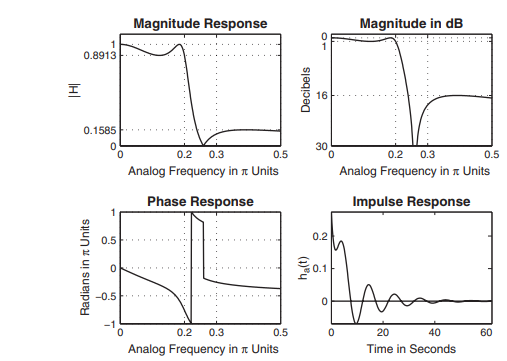
\includegraphics[width=1\linewidth]{Elliptic_lowpass.png}
    \caption{Elliptic}
    \label{fig:enter-label}
\end{figure}
\begin{figure}[H]
    \centering
    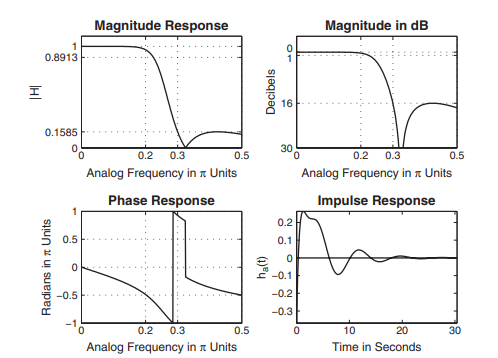
\includegraphics[width=1\linewidth]{Chebyshev2_response.png}
    \caption{Chebshev-II}
    \label{fig:enter-label}
\end{figure}
\begin{figure}[H]
    \centering
    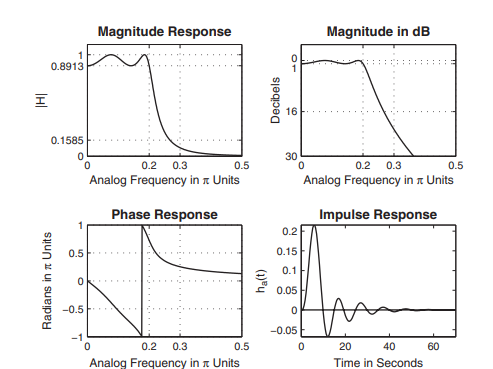
\includegraphics[width=1\linewidth]{Chebyshev1_response.png}
    \caption{Chebyshev-I}
    \label{fig:enter-label}
\end{figure}
\begin{figure}[H]
    \centering
    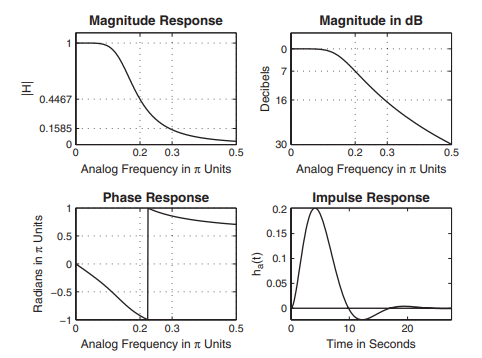
\includegraphics[width=1\linewidth]{Butterworth_response.png}
    \caption{Butterworth}
    \label{fig:enter-label}
\end{figure}
\newpage


\subsection{Analog-Digital Transformation}
After discussing different approaches to the design of analog filters, we
are now ready to transform them into digital filters. These transformations are derived by preserving different aspects of analog and digital filters. If we want to preserve the shape
of the impulse response from analog to digital filter, then we obtain a
technique called impulse invariance transformation. If we want to convert a differential equation representation into a corresponding difference equation representation, then we obtain a finite difference approximation technique. Numerous other techniques are also possible. One technique,
called step invariance, preserves the shape of the step response; this is
explored in Problem P8.24.  Another technique that is similar to the
impulse invariance is the matched-z transformation, which matches the
pole-zero representation. It is described at the end of this section and is
explored in Problem P8.26. The most popular technique used in practice
is called a Bilinear transformation, which preserves the system function
representation from analog to digital domain. In this section, we will
study in detail impulse invariance and bilinear transformations, both of
which can be easily implemented in MATLAB.

\subsubsection{Impulse invariance transformation}
In this design method, we want the digital filter impulse response to look
“similar” to that of a frequency-selective analog filter. Hence we sample
ha(t) at some sampling interval T to obtain h(n); that is,
\begin{equation}
h(n) = h_a(nT)
\end{equation}
In this section, we will use $\Omega$ to represent the analog omega.
The parameter T is chosen so that the shape of ha(t) is “captured” by
the samples. Since this is a sampling operation, the analog and digital
frequencies are related by
\begin{center}
$w = \Omega T$ or $e^{jw}=e^{j\Omega T}$
\end{center}
Since $z = e^{jw}$ on the unit circle and $s= j\Omega$ on the imaginary axis, we have the following transformation from the s-plane to the z-plane
\begin{equation}
z=e^{sT}
\end{equation}
Similarly, 
\begin{equation}
H(z) = \frac{1}{T}\sum_{k=-\infty}^{\infty}H_a(s-j\frac{2\pi}{T}k)
\end{equation}
If $H_a(j\Omega) = H_a(jw/T) = 0$ for $|\Omega| \geq \pi/T$ \\
\begin{center}
    $H(e^{jw})=\frac{1}{T}H_a(jw/T)$, $|w|\leq \pi$
\end{center}
\subsubsection{Design procedure}
Given the digital lowpass filter specifications $w_s, w_p, R_p, A_s$, we want to determine H(z) by first designing the equivalent analog filter and then mapping it into the desired digital filter. The steps required for this procedure are as follows.

\begin{enumerate}
    \item Choose T and determine the analog frequencies
    \begin{center}
        $\Omega_p=\frac{wp}{T_p}$ and $\Omega_s=\frac{w_s}{T}$
    \end{center}
    \item Design an analog filter $H_a(s)$ using the specifications $\Omega_p, \Omega_s, R_p, A_s$, this can be done using any one of the three prototypes (Butterworth, Chebyshev, or Elliptic).
    \item Using partial fraction expansion, expand $H_a(s)$ into 
    \begin{center}
        $$H_a(s) = \sum_{k=1}^{N}\frac{R_k}{s-p_k}$$
    \end{center}
    \item Transform analog poles $p_k$ into digital poles $e^{p_kT}$ to obtain 
    \begin{equation}
        H(z)=\sum_{k=1}^{N}\frac{R_k}{1-e^{p_kT}z^{-1}}
    \end{equation}
\end{enumerate}
\subsubsection{Examples}
Transform 
\begin{center}
$H_a(s) = \frac{s+1}{s^2+5s+6}$
\end{center}
into a digital filter $H(z)$ using the impulse invariance technique in which T = 0.1.\\
\vspace{1em} 
Solution:
\begin{center}
    $H_a(s)=\frac{2}{s+3}+\frac{1}{s+2}$
\end{center}
The poles are at $p_1=-3$ and $p_2=-2$
\begin{center}
    $H(z)=\frac{2}{1-e^{-3T}z^{-1}}-\frac{1}{1-e^{-2T}z^{-1}}=\frac{1-0.8966z^{-1}}{1-1.5595z^{-1}+0.6065z^{-2}}$
\end{center}
the residuez function can be used to convert H(z) into rational function form
\begin{lstlisting}
function [b,a] = imp_invr(c,d,T)
% Impulse invariance transformation from analog to digital filter
% ---------------------------------------------------------------
% [b,a] = imp_invr(c,d,T)
% b = numerator polynomial in z^(-1) of the digital filter
% a = denominator polynomial in z^(-1) of the digital filter
% c = numerator polynomial in s of the analog filter    
% d = denominator polynomial in s of the analog filter
% T = sampling (transformation) parameter
%
[R,p,k] = residue(c,d); p = exp(p*T);
[b,a] = residuez(R,p,k); b = real(b'); a = real(a');
\end{lstlisting}
Verification:
\begin{lstlisting}
 c = [1,1]; d = [1,5,6]; T = 0.1;
 [b,a] = imp_invr(c,d,T)
b = 1.0000 -0.8966
a = 1.0000 -1.5595 0.6065    
\end{lstlisting}
\begin{center}
$$H(z) = \frac{1-0.8966z^{-1}}{1-1.5595z^{-1}+0.6065z^{-2}}$$
\end{center}
Design a lowpass Butterworth prototype to satisfy the following specifications: \\
\vspace{1em}
Passband cutoff: $w_p=0.2\pi$; Passband ripple: $R_p=1$ dB \\
\vspace{1em}
Stopband cutoff: $w_s=0.3\pi$; Stopband ripple: $A_s =15$ dB \\
\vspace{1em}
\begin{lstlisting}
 % Digital filter specifications:
 wp = 0.2*pi; % Digital passband freq in Hz
 ws = 0.3*pi; % Digital stopband freq in Hz
 Rp = 1; % Passband ripple in dB
 As = 15; % Stopband attenuation in dB
 % Analog prototype specifications: Inverse mapping for frequencies
 T = 1; % Set T=1
 OmegaP = wp / T; % Prototype passband freq
 OmegaS = ws / T; % Prototype stopband freq
 % Analog Butterworth prototype filter calculation:
 [cs,ds] = afd_butt(OmegaP,OmegaS,Rp,As);
*** Butterworth Filter Order = 6
 % Impulse invariance transformation:
 [b,a] = imp_invr(cs,ds,T); [C,B,A] = dir2par(b,a)
C = []
B = 1.8557 -0.6304
-2.1428 1.1454
0.2871 -0.4466
A = 1.0000 -0.9973 0.2570
1.0000 -1.0691 0.3699
1.0000 -1.2972 0.6949
\end{lstlisting}
B = Numerator, A= denominator
\begin{center}
$H(z) = \frac{1.8587-0.6304z^{-1}}{1-0.9973z^{-1}+0.257z^{-2}}+\frac{-2.1428 + 1.1454z^{-1}}{1-1.0691z^{-1}+0.3699z^{-2}}+\frac{0.2871-0.4463z^{-1}}{1-1.2972z^{-1}+0.6449z^{-2}}$
\end{center}
Design a lowpass digital filter using a Chebyshev-II prototype to satisfy: \\
\vspace{1em}
Passband cutoff: $w_p=0.2\pi$; Passband ripple: $R_p=1$ dB \\
\vspace{1em}
Stopband cutoff: $w_s=0.3\pi$; Stopband ripple: $A_s =15$ dB \\
\vspace{1em}
\begin{lstlisting}
 % Digital filter specifications:
 wp = 0.2*pi; % Digital passband freq in rad
 ws = 0.3*pi; % Digital stopband freq in rad
 Rp = 1; % Passband ripple in dB
 As = 15; % Stopband attenuation in dB
 % Analog prototype specifications: Inverse mapping for frequencies
 T = 1; % Set T=1
 OmegaP = wp / T; % Prototype passband freq
 OmegaS = ws / T; % Prototype stopband freq
 % Analog Chebyshev-1 prototype filter calculation:
 [cs,ds] = afd_chb2(OmegaP,OmegaS,Rp,As);
*** Chebyshev-2 Filter Order = 4
 % Impulse invariance transformation:
 [b,a] = imp_invr(cs,ds,T); [C,B,A] = dir2par(b,a);    
\end{lstlisting}
Elliptic:
\begin{lstlisting}
 % Digital filter specifications:
 wp = 0.2*pi; % Digital passband freq in rad
 ws = 0.3*pi; % Digital stopband freq in rad
 Rp = 1; % Passband ripple in dB
 As = 15; % Stopband attenuation in dB   
 % Analog prototype specifications: Inverse mapping for frequencies
 T = 1; % Set T=1
 OmegaP = wp / T; % Prototype passband freq
 OmegaS = ws / T; % Prototype stopband freq
 % Analog elliptic prototype filter calculation:
 [cs,ds] = afd_elip(OmegaP,OmegaS,Rp,As);
*** Elliptic Filter Order = 3
 % Impulse invariance transformation:
 [b,a] = imp_invr(cs,ds,T); [C,B,A] = dir2par(b,a);
\end{lstlisting}
The advantages of the impulse invariance mapping are that it is a
stable design and that the frequencies Ω and $w$ are linearly related. But
the disadvantage is that we should expect some aliasing of the analog frequency response, and in some cases this aliasing is intolerable.
Consequently, this design method is useful only when the analog filter is essentially band-limited to a lowpass or bandpass filter in which there
are no oscillations in the stopband.
\subsubsection{Bilinear Transformation}
This mapping is the best transformation method; it involves a well-known
function given by
\begin{equation}
s= \frac{2}{T}\frac{1-z^{-1}}{1+z^{-1}}\rightarrow z=\frac{1+sT/2}{1-sT/2}
\end{equation}
where T is a parameter. Another name for this transformation is the linear
fractional transformation.
\vspace{1em}
Transform $H_a(s) = \frac{s+1}{s^2+5s+6}$ into a digital filter using the bilinear transformation. Choose T = 1.
\begin{center}
$H(z)= H_a(\frac{2}{T}\frac{1-z^{-1}}{1+z^{-1}})= H_a(2\frac{1-z^{-1}}{1+z^{-1}})$ \\
\vspace{1em}
$$H(z)=\frac{2\frac{1-z^{-1}}{1+z^{-1}}+1}{(2\frac{1-z^{-1}}{1+z^{-1}})^2+5(2\frac{1-z^{-1}}{1+z^{-1}})+6}=\frac{0.15+0.1z^{-1}-0.05z^{-2}}{1+0.2z^{-2}}$$ 
\end{center}
The MATLAB program calculates the bilinear transform of the above function given T = 1
\begin{lstlisting}
 c = [1,1]; d = [1,5,6]; T = 1; Fs = 1/T;
 [b,a] = bilinear(c,d,Fs)
b = 0.1500 0.1000 -0.0500
a = 1.0000 0.2000 0.0000    
\end{lstlisting}
$$H(z)=\frac{0.15+0.1z^{-1}-0.05z^{-2}}{1+0.2z^{-2}}$$
\subsubsection{Design Procedure (Bilinear)}
Given the digital lowpass filter specifications $w_s, w_p, R_p, A_s$, we want to determine H(z)
\begin{itemize}
    \item  Choose a value for T. This is arbitrary, and we may set T = 1.
    \item Prewarp the cutoff frequencies $w_p, w_s$ and calculate $\Omega_p, \Omega_p$
    \begin{center}
    $$\Omega_p=\frac{2}{T}\tan(\frac{w_p}{2}), \Omega_s=\frac{2}{T}\tan(\frac{w_s}{2})$$
    \end{center}
    \item Design an analog filter $H_a(s)$ using the specifications $\Omega_p, \Omega_s, R_p, A_s$, this can be done using any one of the three prototypes (Butterworth, Chebyshev, or Elliptic).
    \item Finally, set 
    \begin{center}
        $$H(z)= H_a(\frac{2}{T}\frac{1-z^{-1}}{1+z^{-1}})$$
    \end{center}
\end{itemize}
Design a lowpass Butterworth prototype to satisfy the following specifications: \\
\vspace{1em}
Passband cutoff: $w_p=0.2\pi$; Passband ripple: $R_p=1$ dB \\
\vspace{1em}
Stopband cutoff: $w_s=0.3\pi$; Stopband ripple: $A_s =15$ dB \\
\vspace{1em}
\begin{lstlisting}
 % Digital filter specifications:
 wp = 0.2*pi; % Digital passband freq in rad
 ws = 0.3*pi; % Digital stopband freq in rad
 Rp = 1; % Passband ripple in dB
 As = 15; % Stopband attenuation in dB
 % Analog prototype specifications: Inverse mapping for frequencies
 T = 1; Fs = 1/T; % Set T=1
 OmegaP = (2/T)*tan(wp/2); % Prewarp prototype passband freq
 OmegaS = (2/T)*tan(ws/2); % Prewarp prototype stopband freq
 % Analog Butterworth prototype filter calculation:
 [cs,ds] = afd_butt(OmegaP,OmegaS,Rp,As);
*** Butterworth Filter Order = 6
 % Bilinear transformation:
 [b,a] = bilinear(cs,ds,Fs); [C,B,A] = dir2cas(b,a)
C = 5.7969e-004
B = 1.0000 2.0183 1.0186
1.0000 1.9814 0.9817
1.0000 2.0004 1.0000
A = 1.0000 -0.9459 0.2342
1.0000 -1.0541 0.3753
1.0000 -1.3143 0.7149    
\end{lstlisting}
\begin{center}
 $$H(z)=\frac{0.00057969(1+z^{-1})^6}{(1-0.9459z^{-1}+0.2342z^{-2})(1-1.0541^{-1}+0.3753z^{-2})(1-1.3143^{-1}+0.7149z^{-2})}$$   
\end{center}
\vspace{1em}
Design a lowpass digital filter using a Chebyshev-I prototype to satisfy: \\
\vspace{1em}
Passband cutoff: $w_p=0.2\pi$; Passband ripple: $R_p=1$ dB \\
\vspace{1em}
Stopband cutoff: $w_s=0.3\pi$; Stopband ripple: $A_s =15$ dB \\
\vspace{1em}
\begin{lstlisting}
 % Digital filter specifications:
 wp = 0.2*pi; % Digital passband freq in rad
 ws = 0.3*pi; % Digital stopband freq in rad
 Rp = 1; % Passband ripple in dB
 As = 15; % Stopband attenuation in dB
 % Analog prototype specifications: Inverse mapping for frequencies
 T = 1; Fs = 1/T; % Set T=1
 OmegaP = (2/T)*tan(wp/2); % Prewarp prototype passband freq
 OmegaS = (2/T)*tan(ws/2); % Prewarp prototype stopband freq
 % Analog Chebyshev-1 prototype filter calculation:
 [cs,ds] = afd_chb1(OmegaP,OmegaS,Rp,As);
*** Chebyshev-1 Filter Order = 4
 % Bilinear transformation:
 [b,a] = bilinear(cs,ds,Fs); [C,B,A] = dir2cas(b,a)
C = 0.0018
B = 1.0000 2.0000 1.0000
1.0000 2.0000 1.0000
A = 1.0000 -1.4996 0.8482
1.0000 -1.5548 0.6493    
\end{lstlisting}
Corresponds to the fourth order system defined by:
\begin{center}
    $$H(z)= \frac{0.0018(1+z^{-1})^4}{(1-1.4996z^{-1}+0.8482z^{-2})(1-1.5548z^{-1}+0.5493z^{-2})}$$
\end{center}
Design a lowpass digital filter using a Chebyshev-II prototype to satisfy: \\
\vspace{1em}
Passband cutoff: $w_p=0.2\pi$; Passband ripple: $R_p=1$ dB \\
\vspace{1em}
Stopband cutoff: $w_s=0.3\pi$; Stopband ripple: $A_s =15$ dB \\
\vspace{1em}
\begin{lstlisting}
 % Digital filter specifications:
 wp = 0.2*pi; % Digital passband freq in rad
 ws = 0.3*pi; % Digital stopband freq in rad
 Rp = 1; % Passband ripple in dB
 As = 15; % Stopband attenuation in dB
 % Analog prototype specifications: Inverse mapping for frequencies
 T = 1; Fs = 1/T; % Set T=1
 OmegaP = (2/T)*tan(wp/2); % Prewarp prototype passband freq
 OmegaS = (2/T)*tan(ws/2); % Prewarp prototype stopband freq
 % Analog Chebyshev-2 Prototype Filter Calculation:
 [cs,ds] = afd_chb2(OmegaP,OmegaS,Rp,As);
*** Chebyshev-2 Filter Order = 4
 % Bilinear transformation:
 [b,a] = bilinear(cs,ds,Fs); [C,B,A] = dir2cas(b,a)
C = 0.1797
B = 1.0000 0.5574 1.0000
1.0000 -1.0671 1.0000
A = 1.0000 -0.4183 0.1503
1.0000 -1.1325 0.7183    
\end{lstlisting}
Corresponds to the fourth order system defined by:
\begin{center}
    $$H(z)= \frac{0.1797(1+0.5574z^{-1}+z^{-2})(1-1.0671z^{-1}+z^{-2})}{(1-0.4813z^{-1}+0.1503z^{-2})(1-1.1325z^{-1}+0.7183^{-2})}$$
\end{center}
Elliptic: 
\begin{lstlisting}
 % Digital filter specifications:
 wp = 0.2*pi; % Digital passband freq in rad
 ws = 0.3*pi; % Digital stopband freq in rad
 Rp = 1; % Passband ripple in dB
 As = 15; % Stopband attenuation in dB
 % Analog prototype specifications: Inverse mapping for frequencies
 T = 1; Fs = 1/T; % Set T=1  
 OmegaP = (2/T)*tan(wp/2); % Prewarp prototype passband freq
 OmegaS = (2/T)*tan(ws/2); % Prewarp prototype stopband freq
 % Analog elliptic prototype filter calculation:
 [cs,ds] = afd_elip(OmegaP,OmegaS,Rp,As);
*** Elliptic Filter Order = 3
 % Bilinear transformation:
 [b,a] = bilinear(cs,ds,Fs); [C,B,A] = dir2cas(b,a)
C = 0.1214
B = 1.0000 -1.4211 1.0000
1.0000 1.0000 0
A = 1.0000 -1.4928 0.8612
1.0000 -0.6183 0
\end{lstlisting}
\subsubsection{Matched-z Transform}
This section is very brief because the Matched-z Transform is generally non-suitable because it does not preserve the impulse or frequency response characteristics of the analog filter. Given a root (zero or pole) at the location s = a in the s-plane, we map it in the z-plane at $z=e^{aT}$ where T is a sampling interval. Thus the system function $H_a(s)$ with zeroes {$z_k$} and poles {$p_k$}

\begin{equation}
H_a(s) = \frac{\prod_{k=1}^{M}(s-z_k)}{\prod_{l=1}^{N}(s-p_l)}\rightarrow H(z)=\frac{\prod_{k=1}^{M}(1-e^{z_kT}z^{-1})}{\prod_{l=1}^{N}(s-e^{p_tT}z^{-1})}
\end{equation}
\newpage
\subsection{MATLAB functions for low-pass}
In this section, we will demonstrate the use of MATLAB's filter design
functions to design digital lowpass filters. These functions use the bilinear
transformation because of its desirable advantages as discussed in the
previous section. These functions are as follows.

\begin{enumerate}
    \item Butterworth: [b,a]=butter(N,wn) 
    This function designs an Nth-order lowpass digital Butterworth filter and returns the filter coefficients in length N + 1 vectors b and a. The filter order is given by the N formula for Butterworth, and the cutoff frequency $w_n$ is determined by the prewarping formula. However, in MATLAB all digital frequencies are given in units of $\pi$. Hence $w_n$ is computed by using the following relation:
    \begin{center}
        $w_n=\frac{2}{\pi}\tan^{-1}(\frac{\Omega_cT}{2})$
    \end{center}
    \item Chebyshev-I: [b,a]=cheby1(N,Rp,wn)
    This function designs an Nth-order lowpass digital Chebyshev-I filter
    with Rp decibels of ripple in the passband. It returns the filter coefficients in length N + 1 vectors b and a. The filter order is given by the N formula for Chebyshev-I, and the cutoff frequency $w_n$ is the digital passband frequency
    in units of $\pi$; that is,
    \begin{center}
        $w_n=\frac{w_p}{\pi}$
    \end{center}
    \item Chebyshev-2: [b,a]=cheby2(N,As,wn)
    This function designs an Nth-order lowpass digital Chebyshev-II filter with the stopband attenuation As decibels. It returns the filter coefficients in length N + 1 vectors b and a. The filter order is given by the N formula for Chebyshev-II, and the cutoff frequency $w_n$ is the digital stopband frequency in units of $\pi$; that is,
    \begin{center}
        $w_n=\frac{w_s}{\pi}$
    \end{center}
    \item Elliptic: [b,a]=ellip(N,Rp,As,wn)
    This function designs an Nth-order lowpass digital elliptic filter with the passband ripple of Rp decibels and a stopband attenuation of As decibels. It returns the filter coefficients in length N + 1 vectors b and a. The filter order is given by the N formula for Elliptic, and the cutoff frequency $w_n$ is the digital passband frequency in units of $\pi$; that is
\begin{center}
    $w_n=\frac{w_p}{\pi}$
\end{center}

\end{enumerate}

\newpage
Design a lowpass digital filter using a Butterworth prototype to satisfy: \\
\vspace{1em}
Passband cutoff: $w_p=0.2\pi$; Passband ripple: $R_p=1$ dB \\
\vspace{1em}
Stopband cutoff: $w_s=0.3\pi$; Stopband ripple: $A_s =15$ dB \\
\vspace{1em}
\begin{lstlisting}
 % Digital filter specifications:
 wp = 0.2*pi; % Digital passband freq in rad
 ws = 0.3*pi; % Digital stopband freq in rad
 Rp = 1; % Passband ripple in dB
 As = 15; % Stopband attenuation in dB
 % Analog Prototype Specifications:
 T = 1; % Set T=1
 OmegaP = (2/T)*tan(wp/2); % Prewarp prototype passband freq
 OmegaS = (2/T)*tan(ws/2); % Prewarp prototype stopband freq
 % Analog Prototype Order Calculation:
 N =ceil((log10((10^(Rp/10)-1)/(10^(As/10)-1)))/(2*log10(OmegaP/OmegaS)));
 fprintf('\n*** Butterworth Filter Order = %2.0f \n',N)
** Butterworth Filter Order = 6
 OmegaC = OmegaP/((10^(Rp/10)-1)^(1/(2*N))); % Analog BF prototype cutoff
 wn = 2*atan((OmegaC*T)/2); % Digital BF cutoff freq    
 % Digital butterworth filter design:
 wn = wn/pi; % Digital BF cutoff in pi units
 [b,a]=butter(N,wn); [b0,B,A] = dir2cas(b,a)
C = 5.7969e-004
B = 1.0000 2.0297 1.0300
1.0000 1.9997 1.0000
1.0000 1.9706 0.9709
A = 1.0000 -0.9459 0.2342
1.0000 -1.0541 0.3753
1.0000 -1.3143 0.7149
\end{lstlisting}
\begin{center}
 $$H(z)=\frac{0.00057969(1+z^{-1})^6}{(1-0.9459z^{-1}+0.2342z^{-2})(1-1.0541^{-1}+0.3753z^{-2})(1-1.3143^{-1}+0.7149z^{-2})}$$   
\end{center}
Design a lowpass digital filter using a Chebyshev-I prototype to satisfy: \\
\vspace{1em}
Passband cutoff: $w_p=0.2\pi$; Passband ripple: $R_p=1$ dB \\
\vspace{1em}
Stopband cutoff: $w_s=0.3\pi$; Stopband ripple: $A_s =15$ dB \\
\vspace{1em}
\begin{lstlisting}
 % Digital filter specifications:
 wp = 0.2*pi; % Digital passband freq in rad
 ws = 0.3*pi; % Digital stopband freq in rad
 Rp = 1; % Passband ripple in dB
 As = 15; % Stopband attenuation in dB
 % Analog prototype specifications:
 T = 1; % Set T=1
 OmegaP = (2/T)*tan(wp/2); % Prewarp prototype passband freq
 OmegaS = (2/T)*tan(ws/2); % Prewarp prototype stopband freq
 % Analog prototype order calculation:
 ep = sqrt(10^(Rp/10)-1); % Passband ripple factor
 A = 10^(As/20); % Stopband attenuation factor
 OmegaC = OmegaP; % Analog prototype cutoff freq
 OmegaR = OmegaS/OmegaP; % Analog prototype transition ratio
 g = sqrt(A*A-1)/ep; % Analog prototype intermediate cal.
 N = ceil(log10(g+sqrt(g*g-1))/log10(OmegaR+sqrt(OmegaR*OmegaR-1)));
 fprintf('\n*** Chebyshev-1 Filter Order = %2.0f \n',N)
*** Chebyshev-1 Filter Order = 4
 % Digital Chebyshev-I Filter Design:
 wn = wp/pi; % Digital passband freq in pi units
 [b,a]=cheby1(N,Rp,wn); [b0,B,A] = dir2cas(b,a)    
\end{lstlisting}
\begin{center}
    $$H(z)= \frac{0.0018(1+z^{-1})^4}{(1-1.4996z^{-1}+0.8482z^{-2})(1-1.5548z^{-1}+0.5493z^{-2})}$$
\end{center}
Design a lowpass digital filter using a Chebyshev-II prototype to satisfy: \\
\vspace{1em}
Passband cutoff: $w_p=0.2\pi$; Passband ripple: $R_p=1$ dB \\
\vspace{1em}
Stopband cutoff: $w_s=0.3\pi$; Stopband ripple: $A_s =15$ dB \\
\vspace{1em}
\begin{lstlisting}
 % Digital filter specifications:
 wp = 0.2*pi; % Digital passband freq in rad
 ws = 0.3*pi; % Digital stopband freq in rad
 Rp = 1; % Passband ripple in dB
 As = 15; % Stopband attenuation in dB
 % Analog prototype specifications:
 T = 1; % Set T=1
 OmegaP = (2/T)*tan(wp/2); % Prewarp prototype passband freq
 OmegaS = (2/T)*tan(ws/2); % Prewarp prototype stopband freq
 % Analog prototype order calculation:
 ep = sqrt(10^(Rp/10)-1); % Passband ripple factor
 A = 10^(As/20); % Stopband attenuation factor
 OmegaC = OmegaP; % Analog prototype cutoff freq
 OmegaR = OmegaS/OmegaP; % Analog prototype transition ratio
 g = sqrt(A*A-1)/ep; % Analog prototype intermediate cal.
 N = ceil(log10(g+sqrt(g*g-1))/log10(OmegaR+sqrt(OmegaR*OmegaR-1)));
 fprintf('\n*** Chebyshev-2 Filter Order = %2.0f \n',N)
*** Chebyshev-2 Filter Order = 4
 % Digital Chebyshev-II filter design:
 wn = ws/pi; % Digital stopband freq in pi units
 [b,a]=cheby2(N,As,wn); [b0,B,A] = dir2cas(b,a)
b0 = 0.1797
B = 1.0000 0.5574 1.0000
1.0000 -1.0671 1.0000
A = 1.0000 -0.4183 0.1503
1.0000 -1.1325 0.7183
\end{lstlisting}
\begin{center}
    $$H(z)= \frac{0.1797(1+0.5574z^{-1}+z^{-2})(1-1.0671z^{-1}+z^{-2})}{(1-0.4813z^{-1}+0.1503z^{-2})(1-1.1325z^{-1}+0.7183^{-2})}$$
\end{center}
Elliptic: 
\begin{lstlisting}
 % Digital filter specifications:
 wp = 0.2*pi; % Digital passband freq in rad
 ws = 0.3*pi; % Digital stopband freq in rad
 Rp = 1; % Passband ripple in dB
 As = 15; % Stopband attenuation in dB
 % Analog prototype specifications:
 T = 1; % Set T=1
 OmegaP = (2/T)*tan(wp/2); % Prewarp prototype passband freq
 OmegaS = (2/T)*tan(ws/2); % Prewarp prototype stopband freq
 % Analog elliptic filter order calculations:
 ep = sqrt(10^(Rp/10)-1); % Passband ripple factor
 A = 10^(As/20); % Stopband attenuation factor
 OmegaC = OmegaP; % Analog prototype cutoff freq
 k = OmegaP/OmegaS; % Analog prototype transition ratio
 k1 = ep/sqrt(A*A-1); % Analog prototype intermediate cal.
 capk = ellipke([k.^2 1-k.^2]);
 capk1 = ellipke([(k1 .^2) 1-(k1 .^2)]);
 N = ceil(capk(1)*capk1(2)/(capk(2)*capk1(1)));
 fprintf('\n*** Elliptic Filter Order = %2.0f \n',N)
*** Elliptic Filter Order = 3
 % Digital elliptic filter design:
 wn = wp/pi; % Digital passband freq in pi units
 [b,a]=ellip(N,Rp,As,wn); [b0,B,A] = dir2cas(b,a)
b0 = 0.1214
B = 1.0000 -1.4211 1.0000
1.0000 1.0000 0
A = 1.0000 -1.4928 0.8612
1.0000 -0.6183 0    
\end{lstlisting}
\subsubsection{Comparison of prototypes}
\begin{tabular}{|c|c|c|c|}
\hline
\textbf{Prototype} & \textbf{Order N} & \textbf{Actual $R_p$} & \textbf{Actual $A_s$} \\
\hline
Butterworth & 6 & 1 & 17.6\\
\hline
Chebyshev-I & 4 & 1 & 23.6 \\
\hline
Chebyshev-II & 4 & 0.15 & 15 \\
\hline
Elliptic & 3 & 1 & 16 \\
\hline
\end{tabular} \\
\vspace{1em}
Desired Specs: $w_p=0.2\pi,R_p=1dB,w_s=0.3\pi,A_s=15dB$. Where Rp is the passband ripple measured as wp, and As is the stopband attenuation measured at As. \\
\vspace{1em}
Clearly, the elliptic prototype gives the best design in terms of the
smallest order while satisfying magnitude specifications almost exactly.
However, if we compare phase responses of all four filters, then the elliptic design has the most nonlinear phase response in the passband, while
Butterworth has the least nonlinear phase response.
\newpage
\subsection{Frequency-Band Transformations}
In the preceding two sections, we designed digital lowpass filters from
their corresponding analog filters. Certainly, we would like to design other
types of frequency-selective filters, such as highpass, bandpass, and bandstop. This is accomplished by transforming the frequency axis (or band)
of a lowpass filter so that it behaves as another frequency-selective filter. These transformations on the complex variable z are very similar
to bilinear transformations, and the design equations are algebraic. The
procedure to design a general frequency-selective filter is to first design
a digital prototype (of fixed bandwidth—say, unit bandwidth) lowpass filter and then to apply these algebraic transformations. 
\begin{figure}[H]
    \centering
    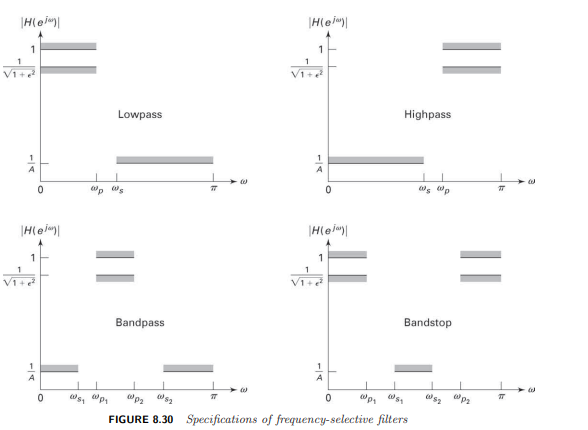
\includegraphics[width=1\linewidth]{FrequencyBand.png}
    \label{fig:enter-label}
\end{figure}
Let $H_{LP}(Z)$ be the given prototype lowpass digital filter, and let H(z) be the desired frequency-selective digital filter. Note that we are using two different frequency variables, Z and z, with $H_{LP}$ and H, respectively 
\begin{center}
$Z^{-1}=G(z^{-1})$
\end{center}
such that 
\begin{center}
$H(z)= H_{LP}(Z)|_{Z^{-1}=G(z^{-1})}$   
\end{center}
Let $w'$ and $w$ be the frequency variables of Z and z, respectively-that is, $Z=e^{jw}$ and $z=e^{jw}$ on their respective unit circles
\begin{figure}[H]
    \centering
    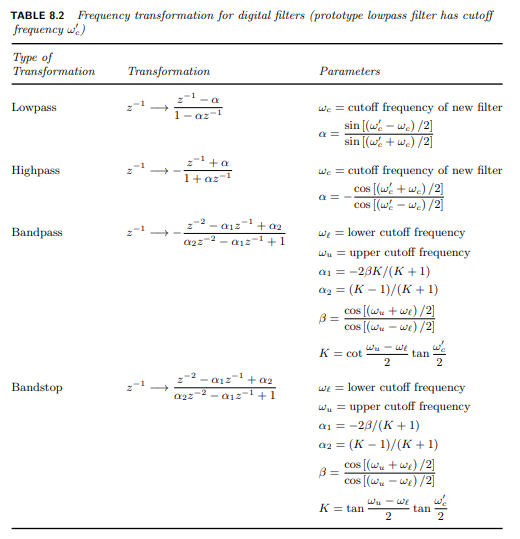
\includegraphics[width=1.1\linewidth]{Frequency_transforms.png}
    \label{fig:enter-label}
\end{figure}
\newpage
Given a Chebyshev-I lowpass with specfications \\
\vspace{1em}
\begin{center}
 $w_p'=0.2\pi$; $R_p=1$ dB \\
\vspace{1em}
 $w_s'=0.3\pi$; $A_s =15$ dB \\
\vspace{1em}    
    $$H_{LP}(Z)= \frac{0.0018(1+Z^{-1})^4}{(1-1.4996Z^{-1}+0.8482Z^{-2})(1-1.5548Z^{-1}+0.5493Z^{-2})}$$
\end{center}

Design a highpass filter with the same parameters but with the passband beginning at $w_p=0.6\pi$
\begin{equation}
\alpha=-\frac{\cos[(0.2\pi+0.6\pi)/2]}{\cos[(0.2\pi-0.6\pi)/2]}=-0.38197
\end{equation}
\begin{center}
$H_{LP}(z)=H(Z)|_{Z=-\frac{z^{-1}-0.38197}{1-0.38197z^{-1}}}$ \\
\vspace{1em}
$$H(z)= \frac{0.02496(1-z^{-1})^4}{(1+0.5561z^{-1}+0.7657z^{-2})(1+1.0416z^{-1}+0.4019z^{-2})}$$
\end{center}
The following MATLAB program is a custom zmapping function to transfrom a lowpass filter to highpass
\begin{lstlisting}
function [bz,az] = zmapping(bZ,aZ,Nz,Dz)
% Frequency-band transformation from Z-domain to z-domain
% -------------------------------------------------------
% [bz,az] = zmapping(bZ,aZ,Nz,Dz)
% performs:
% b(z) b(Z)|
% ---- = ----| N(z)
% a(z) a(Z)|@Z = ----
% D(z)
%
bNzord = (length(bZ)-1)*(length(Nz)-1);
aDzord = (length(aZ)-1)*(length(Dz)-1);
bzord = length(bZ)-1; azord = length(aZ)-1;
bz = zeros(1,bNzord+1);
for k = 0:bzord
    pln = [1];
    for l = 0:k-1
        pln = conv(pln,Nz);
    end
    pld = [1];
    for l = 0:bzord-k-1
        pld = conv(pld,Dz);
    end
    bz = bz+bZ(k+1)*conv(pln,pld);
end
az = zeros(1,aDzord+1);
for k = 0:azord
    pln = [1];
    for l = 0:k-1
        pln = conv(pln,Nz);
    end
    pld = [1];
    for l = 0:azord-k-1
        pld = conv(pld,Dz);
    end
    az = az+aZ(k+1)*conv(pln,pld);
end
\end{lstlisting}
This MATLAB program first creates the analog filter then transforms it into a highpass
\begin{lstlisting}
 % Digital lowpass filter specifications:
 wplp = 0.2*pi; % Digital passband freq in rad
 wslp = 0.3*pi; % Digital stopband freq in rad
 Rp = 1; % Passband ripple in dB
 As = 15; % Stopband attenuation in dB
 % Analog prototype specifications: Inverse mapping for frequencies
 T = 1; Fs = 1/T; % Set T=1
 OmegaP = (2/T)*tan(wplp/2); % Prewarp prototype passband freq
 OmegaS = (2/T)*tan(wslp/2); % Prewarp prototype stopband freq
 % Analog Chebyshev prototype filter calculation:
 [cs,ds] = afd_chb1(OmegaP,OmegaS,Rp,As);
** Chebyshev-1 Filter Order = 4
 % Bilinear transformation:
 [blp,alp] = bilinear(cs,ds,Fs);    
 % Digital highpass filter cutoff frequency:
 wphp = 0.6*pi; % Passband-edge frequency
 % LP-to-HP frequency-band transformation:
 alpha = -(cos((wplp+wphp)/2))/(cos((wplp-wphp)/2))
alpha = -0.3820
 Nz = -[alpha,1]; Dz = [1,alpha];
 [bhp,ahp] = zmapping(blp,alp,Nz,Dz); [C,B,A] = dir2cas(bhp,ahp)
C = 0.0243
B = 1.0000 -2.0000 1.0000
1.0000 -2.0000 1.0000
A = 1.0000 1.0416 0.4019
1.0000 0.5561 0.7647
\end{lstlisting}
\newpage
\subsubsection{MATLAB functions for frequency-selective filters}
\begin{itemize}
    \item Highpass Butterworth: [b,a] = BUTTER(N,wn,'high') designs an Nth-order highpass filter
     with digital 3 dB cutoff frequency wn in units of $\pi$.
     \item Bandpass Butterworth: [b,a] = BUTTER(N,wn,)designs an order 2N bandpass filter if wn is a two-element vector, wn=[w1 w2], with 3 dB passband w1 < w < w2 in units of $\pi$.
     with digital 3 dB cutoff frequency wn in units of $\pi$.
     \item Bandstop Butterworth:[b,a] = BUTTER(N,wn,'stop') is an order 2N bandstop filter if wn=[w1 w2]with 3 dB stopband w1 < w < w2 in units of $\pi$.
\end{itemize}
To design any frequency-selective Butterworth filter, we need to know
the order N and the 3 dB cutoff frequency vector wn. In their SP toolbox, MATLAB provides a function called buttord to compute these parameters. 
\begin{lstlisting}
[N,wn] = buttord(wp,ws,Rp,As)    
\end{lstlisting}
For lowpass filters wp $<$ ws. \\
• For highpass filters wp $>$ ws. \\
• For bandpass filters wp and ws are two-element vectors, wp=[wp1,
wp2] and ws=[ws1,ws2], such that ws1 $<$ wp1 $<$ wp2 $<$ ws2. \\
• For bandstop filters wp1 $<$ ws1 $<$ ws2 $<$ wp2 \\
\vspace{1em}
Similar discussions apply for for cheby1, cheby2, and ellip functions with appropriate modifications.
\vspace{1em}
Chebyshev-I highpass:
\begin{lstlisting}
 % Digital filter specifications: % Type: Chebyshev-I highpass
 ws = 0.4586*pi; % Dig. stopband-edge frequency
 wp = 0.6*pi; % Dig. passband-edge frequency
 Rp = 1; % Passband ripple in dB
 As = 15; % Stopband attenuation in dB
 % Calculations of Chebyshev-I filter parameters:
 [N,wn] = cheb1ord(wp/pi,ws/pi,Rp,As);
 % Digital Chebyshev-I highpass filter design:
 [b,a] = cheby1(N,Rp,wn,'high');
 % Cascade form realization:
 [b0,B,A] = dir2cas(b,a)
b0 = 0.0243
B = 1.0000 -1.9991 0.9991
1.0000 -2.0009 1.0009
A = 1.0000 1.0416 0.4019
1.0000 0.5561 0.7647    
\end{lstlisting}
\begin{center}
$H(z)=\frac{0.0243(1-z^{-1})^4}{(1+0.5661z^{-1}+0.7647z^{-2})(1+1.0416z^{-1}+0.4019z^{-2})}$
\end{center}
Elliptic bandpass: 
\begin{lstlisting}
 % Digital filter specifications: % Type: Elliptic bandpass
 ws = [0.3*pi 0.75*pi]; % Dig. stopband-edge frequency
 wp = [0.4*pi 0.6*pi]; % Dig. passband-edge frequency
 Rp = 1; % Passband ripple in dB
 As = 40; % Stopband attenuation in dB  
 % Calculations of elliptic filter parameters:
 [N,wn] = ellipord(wp/pi,ws/pi,Rp,As);
 % Digital elliptic bandpass filter design:
 [b,a] = ellip(N,Rp,As,wn);
 % Cascade form realization:
 [b0,B,A] = dir2cas(b,a)
b0 = 0.0197
B = 1.0000 1.5066 1.0000
1.0000 0.9268 1.0000
1.0000 -0.9268 1.0000
1.0000 -1.5066 1.0000
A = 1.0000 0.5963 0.9399
1.0000 0.2774 0.7929
1.0000 -0.2774 0.7929
1.0000 -0.5963 0.9399
\end{lstlisting}
Chebyshev-II bandstop 
\begin{lstlisting}
 % Digital filter specifications: % Type: Chebyshev-II bandstop
 ws = [0.4*pi 0.7*pi]; % Dig. stopband-edge frequency
 wp = [0.25*pi 0.8*pi]; % Dig. passband-edge frequency
 Rp = 1; % Passband ripple in dB
 As = 40; % Stopband attenuation in dB
 % Calculations of Chebyshev-II filter parameters:
 [N,wn] = cheb2ord(wp/pi,ws/pi,Rp,As);
 % Digital Chebyshev-II bandstop filter design:
 [b,a] = cheby2(N,As,ws/pi,'stop');
 % Cascade form realization:
 [b0,B,A] = dir2cas(b,a)
b0 = 0.1558
B = 1.0000 1.1456 1.0000
1.0000 0.8879 1.0000
1.0000 0.3511 1.0000
1.0000 -0.2434 1.0000
1.0000 -0.5768 1.0000    
A = 1.0000 1.3041 0.8031
1.0000 0.8901 0.4614
1.0000 0.2132 0.2145
1.0000 -0.4713 0.3916
1.0000 -0.8936 0.7602

\end{lstlisting}

\newpage
\section{Sampling Rate Conversion}
In many practical applications of digital signal processing, one is faced
with the problem of changing the sampling rate of a signal, either increasing it or decreasing it by some amount. The process of converting a signal
from a given rate to a different rate is called sampling rate conversion.
In turn, systems that employ multiple sampling rates in the processing
of digital signals are called multirate digital signal processing systems. In
this chapter, we describe sampling rate conversion and multirate signal
processing in the digital domain.  in which
an analog signal $x_a(t)$ is sampled using the sampling rate of Fs = 1
T
samples/second. The resulting digital signal x(n) is subsequently filtered
using a lowpass filter (LPF) with a cutoff frequency of $\omega_c$.
Thus the output signal y(n) has all its energy in the band 0 $\leq$ $\omega$ $\leq$
$\omega_c = 2\pi fc$. According to the sampling theorem, such a signal may be represented by the rate of 2fc/T samples/second instead of its existing rate
of Fs = 1/T. Note that |fc| $\leq$ 0.5. However, if fc $\leq $ 0.5, then 2fc/T is much less than Fs.
Hence it would seem more advantageous to lower the sampling frequency
to a value closer to 2fc/T and perform signal processing operations at
this lower rate.
Other applications include the need for an optimal interpolation in
computer tomography and efficient multistage designs of narrowband lowpass filters.

\subsection{Motivation}
In modern digital signal processing systems, signals often need to be exchanged between subsystems operating at different sampling rates. Sampling rate conversion addresses this fundamental need by enabling seamless communication between devices or components that process signals at incompatible temporal resolutions.

For example, audio data may be recorded at 48kHz but needs to be played back on systems designed for 44.1kHz. In such cases, direct playback without conversion would introduce aliasing and distortion. Similarly, software-defined radio systems often acquire data at high rates for flexibility but must decimate to lower rates for efficient baseband processing and storage.

Additionally, in multirate DSP systems, sampling rate conversion allows for optimized processing. Lowering the sampling rate reduces computational burden when high-frequency content is not of interest, while increasing the sampling rate (via interpolation) allows signals to be transmitted or synthesized at higher fidelity.

The design of interpolation and decimation filters must account for aliasing and imaging, ensuring that resampling does not degrade signal quality. Sampling rate conversion is therefore a critical operation in applications ranging from telecommunications and audio processing to medical imaging and embedded systems.
\begin{figure}[H]
    \centering
    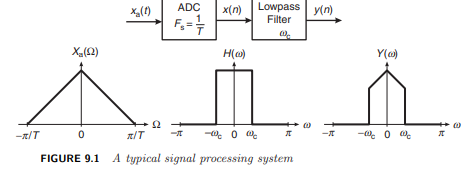
\includegraphics[width=1\linewidth]{TypicalSignalProcessingSystem.png}

\end{figure}
To motivate this concept of interpolation in signal processing, it is
helpful to think of an underlying (or original) analog signal xa(t) that
was sampled to produce the given discrete signal x(n). If the xa(t) was
sampled at the minimum required rate, then, according to the sampling
theorem, it can be recovered completely from the samples x(n). If we now
sample this recovered analog signal, at, say, twice the old rate, we have
succeeded in doubling the sampling rate or interpolating by a factor of 2
with zero interpolation error. Specifically, we have the following. \\
\vspace{1em}
Original discrete signal: 
\begin{equation}
x(n) = x_a(nT)
\end{equation}
Reconstructed analog signal: 
\begin{equation}
x_a(t) = \sum_kx_a(kT)\frac{sin[\pi(t-kT)/T]}{\pi(t-kT)/T}
\end{equation}
Resampled analog signal: \\
\begin{equation}
x_a(m\frac{T}{2})=\sum_kx_a(kT)\frac{sin[\pi(m\frac{T}{2}-kT)/T]}{\pi(m\frac{T}{2}-kT)/T} = \sum_kx_a(kT)\frac{sin[\pi(\frac{m}{2}-k)]}{\pi(\frac{m}{2}-k)}
\end{equation}
This results in the high-rate discrete signal 
\begin{equation}
y(m) = x_a(m\frac{T}{2})
\end{equation}
to the analog signal and then back to the discrete signal at twice the rate.
In the subsequent sections, we will study how to avoid this roundabout
approach and perform sampling rate conversion completely in the digital
domain.
The process of sampling rate conversion in the digital domain can
be viewed as a linear filtering operation, as illustrated in Figure 9.2a.
The input signal x(n) is characterized by the sampling rate $F_x = 1/Tx$,
and the output signal y(m) is characterized by the sampling rate $Fy =
1/T_y$, where Tx and Ty are the corresponding sampling intervals. In our
treatment, the ratio Fy/Fx is constrained to be rational
\begin{equation}
\frac{F_y}{F_x}=\frac{I}{D}
\end{equation}
where D and I are relatively prime integers. We shall show that the
linear filter is characterized by a time-variant impulse response, denoted
\begin{figure}[H]
    \centering
    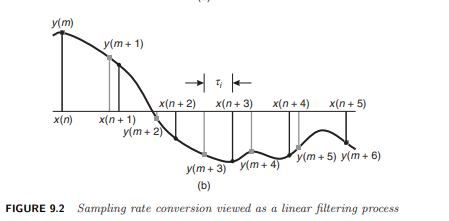
\includegraphics[width=1\linewidth]{SRCasALFP.png}
\end{figure}

The sampling rate conversion process can also be understood from the
point of view of digital resampling of the same analog signal. Let xa(t)
be the analog signal that is sampled at the first rate Fx to generate x(n).
The goal of rate conversion is to obtain another sequence y(m) directly
from x(n), which is equal to the sampled values of xa(t) at a second rate
Fy. As is depicted in Figure 9.2b, y(m) is a time-shifted version of x(n).
Such a time shift can be realized by using a linear filter that has a flat
magnitude response and a linear phase response (i.e., it has a frequency
response of $e^{-j\omega\tau_i}$ , where $\tau_i$ is the time delay generated by the filter). If
the two sampling rates are not equal, the required amount of time shifting
will vary from sample to sample, as shown in Figure 9.2b. Thus the rate
converter can be implemented using a set of linear filters that have the
same flat magnitude response but generate different time delays.
Before considering the general case of sampling rate conversion, we
shall consider two special cases. One is the case of sampling rate reduction
by an integer factor D, and the second is the case of a sampling rate
increase by an integer factor I. The process of reducing the sampling rate
by a factor D (downsampling by D) is called decimation. The process of
increasing the sampling rate by an integer factor I (upsampling by I) is
called interpolation.

\subsection{Decimation by a factor D}
The basic operation required in decimation is the downsampling of the
high-rate signal x(n) into a low-rate signal y(m). We will develop the
time- and frequency-domain relationships between these two signals to
understand the frequency-domain aliasing in y(m). We will then study
the condition needed for error-free decimation and the system structure
required for its implementation.

\subsubsection{Decimation by a factor D}
Note that the downsampled signal y(m) is obtained by selecting one out
of D samples of x(n) and throwing away the other (D - 1) samples out
of every D samples—that is
\begin{equation}
y(m) = x(n)|_{n=mD}=x(mD); n,m,D \in \text{integers}
\end{equation}
The block diagram representation of (9.6) is shown in Figure 9.3. This
downsampling element changes the rate of processing and thus is fundamentally different from other block diagram elements that we have used previously.

\vspace{1em}
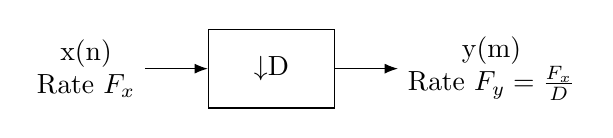
\begin{tikzpicture}[
  node distance=1.8cm and 0.8cm,
  box/.style={draw, minimum width=1.6cm, minimum height=1cm,align=center},
  arrow/.style={-Latex}
]
    

% Nodes
\node[align=center] (n1) {x(n) \\ Rate $F_x$};
\node[box, right=of n1] (n2) {$\downarrow$D};
\node[align=center, right=of n2] (n3) {y(m) \\ Rate $F_y=\frac{F_x}{D}$};


% Pointers
\draw[arrow] (n1) -- (n2);
\draw[arrow] (n2) -- (n3);
\end{tikzpicture}

A downsampling element \\
\vspace{1em}

Using $D = 2$ and $x(n) = \{1, 2, 3, 4, 3, 2, 1 \}$, verify that the downsampler is time
varying.

\begin{center}
$y(m) = x(mD) \Rightarrow y(0) = x(0), y(1)=x(2),y(2)=x(4),y(3)=x(6)$ \\
\vspace{1em}
$y(m) = \{1,3,3,1\}$
\end{center}
\begin{lstlisting}
 x = [1,2,3,4,3,2,1]; y = downsample(x,2)
y =
1331
 x = [1,2,3,4,3,2,1]; y = downsample(x,2,1)
y =
242   
\end{lstlisting}
Visual overview of downsampling:
\begin{figure}[H]
    \centering
    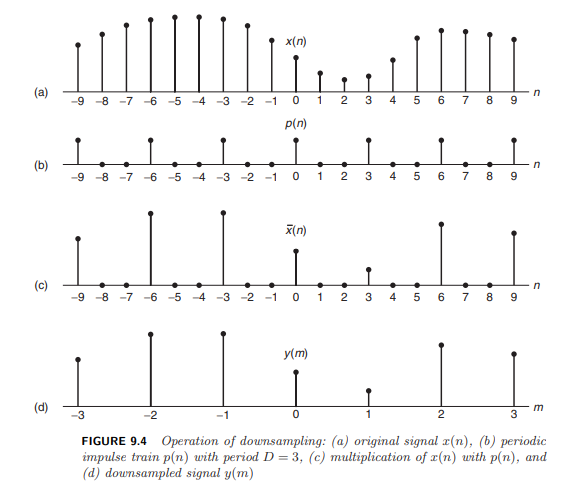
\includegraphics[width=1\linewidth]{DpwmSampling.png}
\end{figure}
Let $x(n) = \cos(0.125\pi n)$. Generate a large number of samples of x(n) and
decimate them using D = 2, 4, and 8 to show the results of decimation. \\
\vspace{1em}
We will plot the middle segments of the signals to avoid end-effects due to
the default lowpass filter in the decimate function. The following MATLAB
script shows details of these operations, and Figure 9.7 shows the plots of the
sequences.
\begin{lstlisting}
n = 0:2048; k1 = 256; k2 = k1+32; m = 0:(k2-k1);
Hf1 = figure('units','inches','position',[1,1,6,4],...
'paperunits','inches','paperposition',[0,0,6,4]);
% (a) Original signal
x = cos(0.125*pi*n); subplot(2,2,1);
Ha = stem(m,x(m+k1+1),'g','filled'); axis([-1,33,-1.1,1.1]);
set(Ha,'markersize',2); ylabel('Amplitude');
title('Original Sequence x(n)','fontsize',TF);
set(gca,'xtick',[0,16,32]); set(gca,'ytick',[-1,0,1]);
% (b) Decimation byD=2
D = 2; y = decimate(x,D); subplot(2,2,2);
Hb = stem(m,y(m+k1/D+1),'c','filled'); axis([-1,33,-1.1,1.1]);
set(Hb,'markersize',2); ylabel('Amplitude');
title('Decimated by D = 2','fontsize',TF);
set(gca,'xtick',[0,16,32]); set(gca,'ytick',[-1,0,1]);
% (c) Decimation byD=4
D = 4; y = decimate(x,D); subplot(2,2,3);
Hc = stem(m,y(m+k1/D+1),'r','filled'); axis([-1,33,-1.1,1.1]);
set(Hc,'markersize',2); ylabel('Amplitude');
title('Decimated by D = 4','fontsize',TF);
set(gca,'xtick',[0,16,32]); set(gca,'ytick',[-1,0,1]);
xlabel('n');
% (d) Decimation byD=8
D = 8; y = decimate(x,D); subplot(2,2,4);
Hd = stem(m,y(m+k1/D+1),'m','filled'); axis([-1,33,-1.1,1.1]);
set(Hd,'markersize',2); ylabel('Amplitude');
title('Decimated by D = 8','fontsize',TF);
set(gca,'xtick',[0,16,32]); set(gca,'ytick',[-1,0,1]);
xlabel('n');
\end{lstlisting}
\begin{figure}[H]
    \centering
    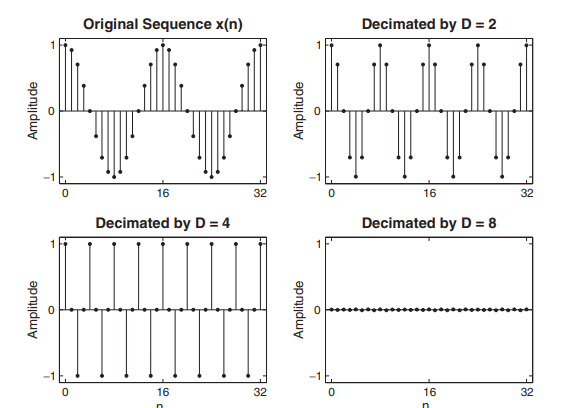
\includegraphics[width=1\linewidth]{DownSamplingExample.png}
\end{figure}
\subsection{Interpolation by a factor I}
An increase in the sampling rate by an integer factor of I—that is,
Fy = IFx can be accomplished by interpolating I - 1 new samples
between successive values of the signal. The interpolation process can
be accomplished in a variety of ways. 
\begin{figure}[H]
    \centering
    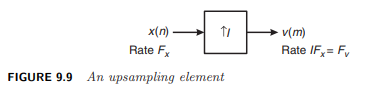
\includegraphics[width=0.75\linewidth]{UpSampling.png}
\end{figure}
MATLAB provides the function [v] =
upsample(x,I) that upsamples input array x into output v by inserting (I-1) zeros between input samples. An optional third parameter,
“phase,” specifies the sample offset, which must be an integer between
0 and (I-1). \\
\vspace{1em}
Let I = 2 and x(n) = \{1, 2, 3, 4\}. The upsampled signal is v(m) = \{1, 0, 2, 0, 3, 0, 4, 0\}
\begin{lstlisting}
  x = [1,2,3,4]; v = upsample(x,3)
v =
100200300400   
\end{lstlisting}
To show its variant
\begin{lstlisting}
 v = upsample(x,3,1)
v =
010020030040
 v = upsample(x,3,2)
v =
001002003004
\end{lstlisting}
\subsubsection{MATLAB Implementation }
MATLAB provides the function [y,h] =
interp(x,I) that resamples the signal in array x at I times the original
sampling rate. The resulting resampled array y is I times longer—that
is, length(y) = I*length(x). The ideal lowpass filter given in (9.30) is
approximated by a symmetric filter impulse response, h, which is designed
internally. It allows the original samples to pass through unchanged and
interpolates between so that the mean square error between them and
their ideal values is minimized. The third optional parameter, L, specifies
the length of the symmetric filter as 2*L*I+1, and the fourth optional
parameter, cutoff, specifies the cutoff frequency of the input signal in $\pi$
units. The default values are L=5 and cutoff = 0.5. Thus, if I=2,
then the length of the symmetric filter is 21 for the default L=5. \\
\vspace{1em}
Let $x(n) = \cos(\pi n)$. Generate samples of x(n) and interpolate them using I = 2,
4, and 8 to show the results of interpolation. 
\begin{center}
We will plot the middle segments of the signals to avoid end-effects due to
the default lowpass filter in the interp function. The following MATLAB
script shows details of these operations, and Figure 9.12 shows the plots of the
sequences.
\end{center}
\begin{lstlisting}
 n = 0:256; k1 = 64; k2 = k1+32; m = 0:(k2-k1);
Hf1 = figure('units','inches','position',[1,1,6,4],...
'paperunits','inches','paperposition',[0,0,6,4]);
% (a) Original signal
x = cos(pi*n); subplot(2,2,1);
Ha = stem(m,x(m+k1+1),'g','filled'); axis([-1,33,-1.1,1.1]);
set(Ha,'markersize',2); ylabel('Amplitude');
title('Original Sequence x(n)','fontsize',TF);
set(gca,'xtick',[0,16,32]); set(gca,'ytick',[-1,0,1]);
% (b) Interpolation byI=2
I = 2; y = interp(x,I); subplot(2,2,2);
Hb = stem(m,y(m+k1*I+1),'c','filled'); axis([-1,33,-1.1,1.1]);
set(Hb,'markersize',2); ylabel('Amplitude');
title('Interpolated by I = 2','fontsize',TF);
set(gca,'xtick',[0,16,32]); set(gca,'ytick',[-1,0,1]);
% (c) Interpolation byI=4
I = 4; y = interp(x,I); subplot(2,2,3);
Hc = stem(m,y(m+k1*I+1),'r','filled'); axis([-1,33,-1.1,1.1]);
set(Hc,'markersize',2); ylabel('Amplitude');
title('Interpolated by I = 4','fontsize',TF);
set(gca,'xtick',[0,16,32]); set(gca,'ytick',[-1,0,1]);
xlabel('n');
% (d) Interpolation byI=8
I = 8; y = interp(x,I); subplot(2,2,4);
Hd = stem(m,y(m+k1*I+1),'m','filled'); axis([-1,33,-1.1,1.1]);
set(Hd,'markersize',2); ylabel('Amplitude');
title('Interpolated by I = 8','fontsize',TF);
set(gca,'xtick',[0,16,32]); set(gca,'ytick',[-1,0,1]);
xlabel('n');
\end{lstlisting}
Examine the frequency response of the lowpass filter used in the interpolation
of the signal 
\begin{lstlisting}
n = 0:256; x = cos(pi*n); w = [0:100]*pi/100;
Hf1 = figure('units','inches','position',[1,1,6,4],...
'paperunits','inches','paperposition',[0,0,6,4]);
% (a) Interpolation by I = 2, L = 5;
I = 2; [y,h] = interp(x,I); H = freqz(h,1,w); H = abs(H);
subplot(2,2,1); plot(w/pi,H,'g'); axis([0,1,0,I+0.1]); ylabel('Magnitude');
title('I = 2, L = 5','fontsize',TF);
set(gca,'xtick',[0,0.5,1]); set(gca,'ytick',[0:1:I]);
% (b) Interpolation by I = 4, L = 5;
I = 4; [y,h] = interp(x,I); H = freqz(h,1,w); H = abs(H);
subplot(2,2,2); plot(w/pi,H,'g'); axis([0,1,0,I+0.2]); ylabel('Magnitude');
title('I = 4, L = 5','fontsize',TF);
set(gca,'xtick',[0,0.25,1]); set(gca,'ytick',[0:1:I]);
% (c) Interpolation by I = 8, L = 5;
I = 8; [y,h] = interp(x,I); H = freqz(h,1,w); H = abs(H);
subplot(2,2,3); plot(w/pi,H,'g'); axis([0,1,0,I+0.4]); ylabel('Magnitude');
title('I = 8, L = 5','fontsize',TF); xlabel('\omega/\pi','fontsize',10)
set(gca,'xtick',[0,0.125,1]); set(gca,'ytick',[0:2:I]);
% (d) Interpolation by I = 8, L = 10;
I = 8; [y,h] = interp(x,I,10); H = freqz(h,1,w); H = abs(H);
subplot(2,2,4); plot(w/pi,H,'g'); axis([0,1,0,I+0.4]); ylabel('Magnitude');
title('I = 8, L = 10','fontsize',TF); xlabel('\omega/\pi','fontsize',10)
set(gca,'xtick',[0,0.125,1]); set(gca,'ytick',[0:2:I]);
\end{lstlisting}
\subsection{Sampling Rate Conversion by a rational factor I/D}
Having discussed the special cases of decimation (downsampling by a factor D) and interpolation (upsampling by a factor I), we now consider
the general case of sampling rate conversion by a rational factor I/D.
Basically, we can achieve this sampling rate conversion by first performing interpolation by the factor I and then decimating the output of the
interpolator by the factor D. In other words, a sampling rate conversion
by the rational factor I/D is accomplished by cascading an interpolator
with a decimator.
\begin{figure}[H]
    \centering
    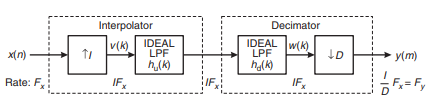
\includegraphics[width=0.5\linewidth]{CascadeID.png}
\end{figure}
\subsubsection{MATLAB Implementation}
MATLAB Implementation MATLAB provides the function [y,h]=
resample(x,I,D) that resamples the signal in array x at I/D times
the original sampling rate. The resulting resampled array y is I/D times
longer (or the ceiling of it if the ratio is not an integer)—that is,
length(y) = ceil(I/D)*length(x). The function approximates the
anti-aliasing (lowpass) filter given in (9.36) by an FIR filter, h, designed
(internally) using the Kaiser window. It also compensates for the filter's
delay. The length of the FIR filter h that resample uses is proportional to
the fourth (optional) parameter L that has the default value of 10. For
L=0, resample performs a nearest-neighbor interpolation. The fifth optional parameter beta (default value 5) can be used to specify the Kaiser
window stopband attenuation parameter $\beta$. The filter characteristics can
be studied using the impulse response h. \\
\vspace{1em}
Consider the sequence $x(n) = \cos(0.125\pi n)$ discussed in Example 9.2. Change
its sampling rate by 3/2, 3/4, and 5/8.
\begin{lstlisting}
n = 0:2048; k1 = 256; k2 = k1+32; m = 0:(k2-k1);
% (a) Original signal
x = cos(0.125*pi*n);
% (b) Sample rate conversion by 3/2: I= 3,D=2
I = 3; D = 2; y = resample(x,I,D);
% (c) Sample rate conversion by 3/4: I= 3,D=4
I = 3; D = 4; y = resample(x,I,D);
% (d) Sample rate conversion by 5/8: I= 5,D=8
I = 5; D = 8; y = resample(x,I,D);
% Plotting commands follow
\end{lstlisting}
\begin{figure}[H]
    \centering
    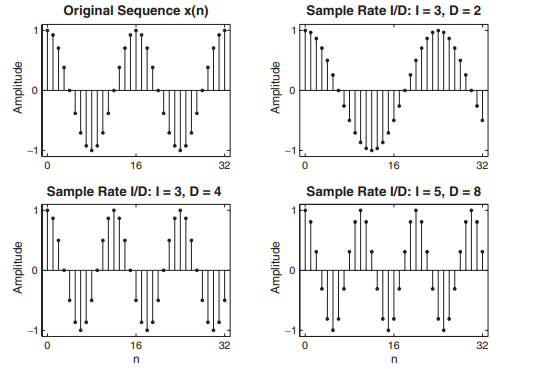
\includegraphics[width=1\linewidth]{RationalFactor.png}
\end{figure}
\subsection{FIR Designs for Sampling Rate Conversion}
In practical implementations of sampling rate converters, we must replace
the ideal lowpass filters of previously used equations by a practical finite-order filter. The lowpass filter can be designed to have linear
phase, a specified passband ripple, and stopband attenuation. Any of the
standard, well-known FIR filter design techniques (e.g., window method,
frequency-sampling method) can be used to carry out this design. We
consider linear-phase FIR filters for this purpose because of their ease
of design and because they fit very nicely into a decimator stage where
only one of D outputs is required on. We will first discuss integer interpolators, followed by integer
decimators and then the rational resamplers.

\subsubsection{FIR Integer Interpolation}
The frequency response of a FIR Integer interpolator is 
\begin{equation}
H(\omega) = \begin{cases}
I, & |\omega| < \pi/4 \\
0, & \text{otherwise}
\end{cases}
\end{equation}
\begin{figure}[H]
    \centering
    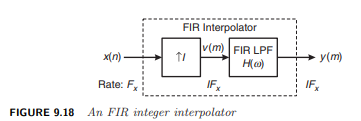
\includegraphics[width=0.75\linewidth]{FIR_Interpolator.png}
\end{figure}
\subsubsection{MATLAB implementation of FIR Interpolator}
To design a linear-phase FIR filter for
use in interpolation (and, as we shall see later, for decimation) operation,
MATLAB provides the function h = intfilt(I,L,alpha). When used
on a sequence interspersed with I-1 consecutive zeros between every
I samples, the function performs ideal bandlimited interpolation using
the nearest 2*L nonzero samples. It assumes that the bandwidth of the
signal x(n) is alpha times $\pi$ radians/sample—that is, alpha=1 means the
full signal bandwidth. The length of the filter impulse response array h
is 2*I*L-1. The designed filter is identical to that used by the interp
function. Therefore, the parameter L should be chosen carefully to avoid
numerical instability. It should be a smaller value for higher I value but
no more than 10. \\
\vspace{1em}
Design a linear-phase FIR interpolation filter to interpolate a signal by a factor of 4, using the bandlimited method.
\begin{lstlisting}
I = 4; L = 5;
% (a) Full signal bandwidth: alpha = 1
alpha = 1; h = intfilt(I,L,alpha);
[Hr,w,a,L] = Hr_Type1(h); Hr_min = min(Hr); w_min = find(Hr == Hr_min);
H = abs(freqz(h,1,w)); Hdb = 20*log10(H/max(H)); min_attn = Hdb(w_min);
% (b) Partial signal bandwidth: alpha = 0.75
alpha = 0.75; h = intfilt(I,L,alpha);
[Hr,w,a,L] = Hr_Type1(h); Hr_min = max(Hr(end/2:end)); w_min = find(Hr == Hr_min);
H = abs(freqz(h,1,w)); Hdb = 20*log10(H/max(H)); min_attn = Hdb(w_min);
% Plotting commands follow
\end{lstlisting}
In the following example, we design a linear-phase equiripple FIR
interpolation filter using the Parks–McClellen algorithm. \\
\vspace{1em}
Design an interpolator that increases the input sampling rate by a factor of
I = 5. Use the firpm algorithm to determine the coefficients of the FIR filter
that has 0.1 dB ripple in the passband and is down by at least 30 dB in the
stopband. Choose reasonable values for band-edge frequencies.
\begin{lstlisting}
I = 5; Rp = 0.1; As = 30; wp = pi/I; ws = wp+pi*0.12;
[delta1,delta2] = db2delta(Rp,As); weights = [delta2/delta1,1];
F = [0,wp,ws,pi]/pi; A = [I,I,0,0];
h = firpm(30,F,A,weights); n = [0:length(h)-1];
[Hr,w,a,L] = Hr_Type1(h); Hr_min = min(Hr); w_min = find(Hr == Hr_min);
H = abs(freqz(h,1,w)); Hdb = 20*log10(H/max(H)); min_attn = Hdb(w_min); 
\end{lstlisting}
Let x(n) = cos(0.5$\pi$n). Increase the input sampling rate by a factor of I = 5,
using the filter designed in previous example.
\begin{lstlisting}
% Given Parameters:
I = 5; Rp = 0.1; As = 30; wp = pi/I; ws = 0.32*pi;
[delta1,delta2] = db2delta(Rp,As); weights = [delta2/delta1,1];
n = [0:50]; x = cos(0.5*pi*n);
n1 = n(1:17); x1 = x(17:33); % For plotting purposes
% Input signal plotting commands follow
% Interpolation with Filter Design: Length M = 31
M = 31; F = [0,wp,ws,pi]/pi; A = [I,I,0,0];
h = firpm(M-1,F,A,weights); y = upfirdn(x,h,I);
delay = (M-1)/2; % Delay imparted by the filter
m = delay+1:1:50*I+delay+1; y = y(m); m = 1:81; y = y(81:161); % for plotting
% Output signal plotting commands follow
\end{lstlisting}
\subsubsection{Design specifications}
When we replace $H_1(\omega)$ by a finite-order FIR filter $H(\omega)$, we must allow
for a transition band; thus the filter cannot have a passband edge up to
$\pi$/I. Toward this, we define \\
 $w_{x,p}$ as the highest frequency of the signal x(n) that we want to preserve, and \\
$w_{x,s}$  as the full signal bandwidth of x(n),—that is, there is no energy
in x(n) above the frequency $\omega$x,s.
\begin{figure}[H]
    \centering
    \label{fig:enter-label}
\end{figure}
FIR filter can now be designed to pass frequencies up to $w$x,p/I and to
suppress frequencies starting at (2$\pi$ - $\omega$x,s)/I. Let
\begin{equation}
w_p=\frac{w_{x,p}}{I}, w_s=(\frac{2\pi-w_{x,s}}{I})
\end{equation}
\begin{equation}
H(\omega) = H_r(\omega)e^{j\theta(w)}
\end{equation}
Design a better FIR lowpass filter for sampling rate increase by a factor of I = 5
for the signal in the previous example
\begin{lstlisting}
% Given Parameters:
n = [0:50]; wxp = 0.5*pi; x = cos(wxp*n);
n1 = n(1:9); x1 = x(9:17); % for plotting purposes
I = 5; I = 5; Rp = 0.01; As = 50; wp = wxp/I; ws = (2*pi-wxp)/I;
[delta1,delta2] = db2delta(Rp,As); weights = [delta2/delta1,1];
[N,Fo,Ao,weights] = firpmord([wp,ws]/pi,[1,0],[delta1,delta2],2);N = N+2;
% Input signal plotting commands follow
% Interpolation with Filter Design: Length M = 31
h = firpm(N,Fo,I*Ao,weights); y = upfirdn(x,h,I);
delay = (N)/2; % Delay imparted by the filter
m = delay+1:1:50*I+delay+1; y = y(m); m = 0:40; y = y(81:121);
% Output signal plotting commands follow
[Hr,w,a,L] = Hr_Type1(h); Hr_min = min(Hr); w_min = find(Hr == Hr_min);
H = abs(freqz(h,1,w)); Hdb = 20*log10(H/max(H)); min_attn = Hdb(w_min);
% Filter design plotting commands follow
\end{lstlisting}
\subsubsection{FIR Integer Decimation}
\begin{figure}{h}
    \centering
    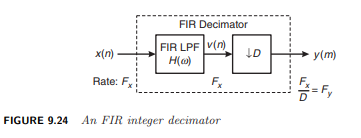
\includegraphics[width=0.75\linewidth]{FIR_Decimator.png}
\end{figure}
Condition to avoid aliasing:
\begin{equation}
H(\omega)X(\omega) = 0, \space \text{for} \space \frac{\pi}{D}\leq |\omega| \leq \pi
\end{equation}
\begin{equation}
Y(\omega_y)= \frac{1}{D}X(\omega)H(\omega)
\end{equation}
Design a decimator that downsamples an input signal x(n) by a factor D = 2.
Use the firpm algorithm to determine the coefficients of the FIR filter that has
a 0.1 dB ripple in the passband and is down by at least 30 dB in the stopband.
Choose reasonable values for band-edge frequencies.
\begin{lstlisting}
% Filter Design
D = 2; Rp = 0.1; As = 30; wp = pi/D; ws = wp+0.1*pi;
[delta1,delta2] = db2delta(Rp,As);
[N,F,A,weights] = firpmord([wp,ws]/pi,[1,0],[delta1,delta2],2);
h = firpm(N,F,A,weights); n = [0:length(h)-1];
[Hr,w,a,L] = Hr_Type1(h); Hr_min = min(Hr); w_min = find(Hr == Hr_min);
H = abs(freqz(h,1,w)); Hdb = 20*log10(H/max(H)); min_attn = Hdb(w_min);
% Plotting commands follow
\end{lstlisting}
\subsubsection{MATLAB implementation for FIR Decimation}
As discussed, the upfirdn function can
also be used for implementing the user-designed FIR filter in the decimation operation. When invoked as y = upfirdn(x,h,1,D), the function
filters the signal data in the array x with the impulse response given in the
array h and then downsamples the filtered data by the integer factor D to
produce the output array y, thus implementing the system in Figure 9.24. \\
\vspace{1em}
Using the filter designed in Example 9.11, decimate sinusoidal signals $x_1(n) =
\cos(\pi n/8), x_2(n) = cos(\pi n/2)$ with frequencies within the passband of
the filter. Verify the performance of the FIR filter and the results of the
decimation.
\begin{lstlisting}
 % Given Parameters:
D = 2; Rp = 0.1; As = 30; wp = pi/D; ws = wp+0.1*pi;
% Filter Design
[delta1,delta2] = db2delta(Rp,As);
[N,F,A,weights] = firpmord([wp,ws]/pi,[1,0],[delta1,delta2],2);
h = firpm(N,F,A,weights); delay = N/2; % Delay imparted by the filter
% Input signal x1(n) = cos(2*pi*n/16)
n = [0:256]; x = cos(pi*n/8);
n1 = n(1:33); x1 = x(33:65); % for plotting purposes
% Input signal plotting commands follow
% Decimation of x1(n):D=2
y = upfirdn(x,h,1,D);   
m = delay+1:1:128/D+delay+1; y = y(m); m = 0:16; y = y(16:32);
% Output signal plotting commands follow
% Input signal x2(n) = cos(8*pi*n/16)
n = [0:256]; x = cos(8*pi*n/(16));
n1 = n(1:33); x1 = x(33:65); % for plotting purposes
% Input signal plotting commands follow
% Decimation of x2(n):D=2
y = upfirdn(x,[h],1,D); %y = downsample(conv(x,h),2);
m = delay+1:1:128/D+delay+1; y = y(m); m = 0:16; y = y(16:32);
% Output signal plotting commands follow
\end{lstlisting}
\subsubsection{Design Specifications}
\begin{equation}
w_p=w_{x,p}, w_s=(\frac{2\pi}{D}-\omega_{x,s})
\end{equation}
wx,s as the frequency above which aliasing error is tolerated.
\begin{lstlisting}
% Given Parameters:
D = 2; Rp = 0.1; As = 50; wxp = pi/8; wxs = pi/D; wp = wxp; ws = (2*pi/D)-wxs;
% Filter Design
[delta1,delta2] = db2delta(Rp,As);
[N,F,A,weights] = firpmord([wp,ws]/pi,[1,0],[delta1,delta2],2); N = ceil(N/2)*2;
h = firpm(N,F,A,weights); delay = N/2; % Delay imparted by the filter
% Input signal x(n) = cos(2*pi*n/16)
n = [0:256]; x = cos(pi*n/8);
n1 = n(1:33); x1 = x(33:65); % for plotting purposes
% Input signal plotting commands follow
% Decimation of x(n):D=2
y = upfirdn(x,h,1,D);
m = delay+1:1:128/D+delay+1; y1 = y(m); m = 0:16; y1 = y1(14:30);
% Output signal plotting commands follow
% Filter Design Plots
[Hr,w,a,L] = Hr_Type1(h); Hr_min = min(Hr); w_min = find(Hr == Hr_min);
H = abs(freqz(h,1,w)); Hdb = 20*log10(H/max(H)); min_attn = Hdb(w_min);
% Filter design plotting commands follow
\end{lstlisting}
\subsubsection{FIR Rational-Rate Conversion}
\begin{equation}
H(\omega) = \begin{cases}
I, & 0 \leq |\omega| \leq \text{min}(\pi/D,\pi/I) \\
0, & \text{otherwise}
\end{cases}
\end{equation}
For the signal x(n) we define
• $w_{x,p}$ as the signal bandwidth that should be preserved,
• $w_{x,s_1}$ as the overall signal bandwidth, and
• $w_{x,s_1}$ as the signal bandwidth that is required to be free of aliasing error
after resampling.
\begin{equation}
0 < \omega_{x,p}\leq\omega_{x,s_2}\leq \frac{I\pi}{D} \space \text{and} \space \omega_{x,s_1} \leq \pi
\end{equation}
\begin{equation}
w_p = (\frac{w_{x,p}}{I}), w_s=min[\frac{2\pi}{I}-\frac{w_{x,s_1}}{I},\frac{2\pi}{D}-\frac{w_{x,s_2}}{I}]
\end{equation}
\subsubsection{MATLAB implementation for FIR rational conversion}
n Clearly, the upfirdn function implements
all the necessary operations needed in the rational sampling rate conversion system shown in Figure 9.28. When invoked as y = upfirdn(x,h,
I,D), it performs a cascade of three operations: upsampling the input data
array x by a factor of the integer I, FIR filtering the upsampled signal data
with the impulse response sequence given in the array h, and, finally, downsampling the result by a factor of the integer D. Using a well-designed filter,
we have complete control over the sampling rate conversion operation. \\
\vspace{1em}
A signal x(n) has a total bandwidth of 0.9$\pi$. It is resampled by a factor of
4/3 to obtain y(m). We want to preserve the frequency band up to 0.8$\pi$ and
require that the band up to 0.7$\pi$ be free of aliasing. Using the Parks–McClellan
algorithm, determine the coefficients of the FIR filter that has 0.1 dB ripple in
the passband and 40 dB attenuation in the stopband.
\begin{lstlisting}
% Given Parameters:
I = 4; D = 3; Rp = 0.1; As = 40;
wxp = 0.8*pi; wxs1 = 0.9*pi; wxs2 = 0.7*pi;
% Computed Filter Parameters
wp = wxp/I; ws = min((2*pi/I-wxs1/I),(2*pi/D-wxs2/I));
% Filter Design
[delta1,delta2] = db2delta(Rp,As);
[N,F,A,weights] = firpmord([wp,ws]/pi,[1,0],[delta1,delta2],2);
N = ceil(N/2)*2+1; h = firpm(N,F,I*A,weights);
[Hr,w,a,L] = Ampl_res(h); Hr_min = min(Hr); w_min = find(Hr == Hr_min);
H = abs(freqz(h,1,w)); Hdb = 20*log10(H/max(H)); min_attn = Hdb(w_min);
% Plotting commands follow
\end{lstlisting}
\begin{figure}[H]
    \centering
    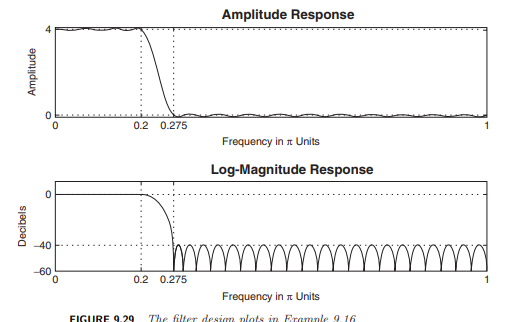
\includegraphics[width=0.75\linewidth]{FIR_Rational.png}
\end{figure}



\newpage

\section{Round-Off Effects for Digital Filters (unfinished)}
We begin by discussing analog-to-digital (A/D) conversion noise using the number representations and quantization error characteristics developed in Chapter 6. We then analyze the multiplication and addition
quantization (collectively known as arithmetic round-off error) models.
The effects of these errors on filter output are discussed as two topics:
correlated errors called limit cycles and uncorrelated round-off noise.

\subsection{Motivation}
Suppose your implementing DSP on a hardware, using a microcontroller. There are some parameters you need to consider:
\begin{itemize}
    \item Clock Speed (MHz) - Determines how fast instructions are executed  faster = more samples per second
    \item Data Width (8/16/32-bit) - Wider registers handle larger numbers and more precise calculations, key for filtering, FFTs, etc.
    \item Floating Point Unit (FPU) - Allows fast floating-point operations — critical for high-resolution DSP (IIR, FFT, ML, etc.)
    \item DSP Extensions / SIMD - Includes hardware MAC (multiply-accumulate), barrel shifters, and parallel ops — drastically speeds up filters and convolutions
    \item RAM \& Flash Size - You need RAM for buffering/filter taps and Flash for program + coefficients
    \item DMA (Direct Memory Access) - Allows data transfers without CPU load — useful in streaming DSP pipelines
    \item Interrupt Latency \& Timer Precision - Key for real-time signal sampling and scheduling DSP tasks accurately
\end{itemize}

\subsubsection{Examples of microcontrollers that could be used}


\begin{tabularx}{\textwidth}{|c|X|X|X|X|}
\hline
\textbf{Processor Type} & \textbf{Examples} & \textbf{DSP Capability}  \\
\hline
8-bit MCU & ATmega328P (Arduino Uno) & Very limited — only basic filters with fixed-point math \\
\hline
16-bit MCU & MSP430, dsPIC & Moderate — can do more, but lacks FPU, slow for audio/DSP \\
\hline
32-bit MCU (no FPU) & Cortex-M0/M3 (STM32F1, Arduino Due) & Basic DSP with fixed-point — slow for FFT/IIR \\
\hline
32-bit MCU (with FPU) & Cortex-M4/M7 (Teensy, STM32F4/7, Portenta H7) &  Excellent — fast FIR, IIR, FFT, ML possible \\
\hline
DSP cores (dedicated) & TI C2000, Analog Devices SHARC, XMOS & Designed for DSP — used in audio, radar, control systems \\
\hline
Application Processors & ARM A53 (Raspberry Pi), Intel x86 &  Extreme DSP power — real-time limits unless RTOS used \\
\hline
\end{tabularx}
If you only had an Arduino Uno available to use for DSP (specifically ADC \& DAC), round-off effects would need to be studied to ensure the most accurate results. Since the quantizer (Arduino) is only 8 bits in data width and has no FPU, if it were to be used as ADC and your input was 4.43 V for instance, it would be rounded to another voltage level.
\subsection{Analysis of A/D Quantization noise}
From the quantizer characteristics obtained in Chapter 6, it is obvious
that the quantized value Q[x] is a nonlinear operation on the value x.
Hence the exact analysis of the finite word-length effects in digital filters
is generally difficult and one has to consider less ideal analysis techniques
that work well in practice. One such technique is the statistical modeling technique. It converts
the nonlinear analysis problem into a linear one and allows us to examine output-error characteristics. In this technique, we assume that the quantized value Q[x] is a sum of the exact value x and the quantization error e, When x(n) is applied as an
input sequence to the quantizer, the error e(n) is assumed to be a random
sequence. We then develop a statistical model for this random sequence
to analyze its effects through a digital filter.
For the purpose of analysis, we assume that the quantizer employs
fixed-point two's-complement number format representation. Using the
results given previously, we can extend this analysis to other formats as
well.

\subsubsection{Statistical Model}
\begin{figure}[H]
    \centering
    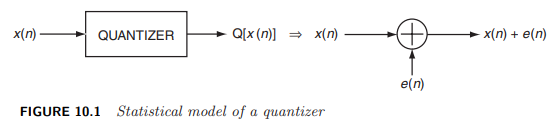
\includegraphics[width=0.75\linewidth]{StatisticalQuantizer.png}
\end{figure}
We model the quantizer block on the input as a signal-plus-noise
operation—that is
\begin{equation}
Q[x(n)]=x(n)+e(n)
\end{equation}
where e(n) is a random sequence that describes the quantization error sequence and is termed the quantization noise \\
\vspace{1em}
Model Assumptions
\begin{itemize}
    \item The sequence e(n) is a sample sequence from a stationary random
process \{e(n)\}.
    \item . This random process \{e(n)\} is uncorrelated with sequence x(n).
    \item The process \{e(n)\} is an independent process (i.e., the samples are
    independent of each other)
    \item The probability density function (pdf), $f_E(e)$, of sample e(n) for each
n is uniformly distributed over the interval of width $\Delta$ = $2^{-B}$, which
is the quantizer resolution.
\end{itemize}
\subsubsection{Analysis using MATLAB}
To investigate the statistical properties of the error samples, we will have
to generate a large number of these samples and plot their distribution
using a histogram (or a probability bar graph). Furthermore, we have to
design the sequence x(n) so that its samples do not repeat; otherwise, the
error samples will also repeat, which will result in an inaccurate analysis. This can be guaranteed either by choosing a well-defined aperiodic
sequence or a random sequence.
We will quantize x(n) using B-bit rounding operation. A similar implementation can be developed for the truncation operation. e(n) is the normalized error and is uniformly distributed over the interval $[-\Delta/2,\Delta/2]$.
\begin{equation}
e_1(n) = e(n)2^B \rightarrow e_1(n)\in[-1/2,1/2]
\end{equation}
$e_2(n)$ is the average of two consecutive normalized error samples. 
\begin{equation}
e_2(n) = \frac{e_1(n)+e_1(n-1)}{2}
\end{equation}
\begin{figure}[H]
    \centering
    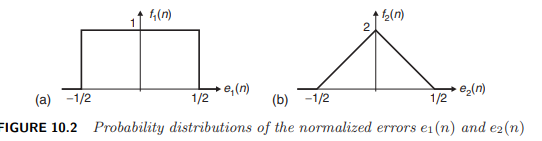
\includegraphics[width=0.5\linewidth]{E1E2.png}
\end{figure}
\begin{lstlisting}
function [H1,H2,Q, estat] = StatModelR(xn,B,N);
% Statistical Model (Rounding) for A/D Quantization error and its Distribution
% ------------- -------------------------------------------------------------
% [H1,H2,Q] = StatModelR(xn,B,N);
% OUT: H1 = normalized histogram of e1
% H2 = normalized histogram of e2
% Q = normalized histogram bins
% estat = row vector: [[e1avg,e1std,e2avg,e2std]
% IN: B = bits to quantize
% N = number of samples of x(n)
% xn = samples of the sequence
% Plot variables
bM = 7; DbM = 2^bM; % Bin parameter
M = round((DbM)/2); % Half number of bins
bins = [-M+0.5:1:M-0.5]; % Bin values from -M to M
Q = bins/(DbM); % Normalized bins
% Quantization error analysis
xq = (round(xn*(2^B)))/(2^B); % Quantized to B bits
e1 = xq-xn; clear xn xq; % Quantization error
e2 = 0.5*(e1(1:N-1)+e1(2:N)); % Average of two adj errors
e1avg = mean(e1); e1std = std(e1); % Mean & std dev of the error e1
e2avg = mean(e2); e2std = std(e2); % Mean & std dev of the error e2
estat = [e1avg,e1std,e2avg,e2std];
% Probability distribution of e1
e1 = floor(e1*(2^(B+bM))); % Normalized e1 (int between -M & M)
e1 = sort([e1,-M-1:1:M]); %
H1 = diff(find(diff(e1)))-1; clear e1; % Error histogram
if length(H1) == DbM+1
H1(DbM) = H1(DbM)+H1(DbM+1);
H1 = H1(1:DbM);
end
H1 = H1/N; % Normalized histogram
% Probability distribution of e2
e2 = floor(e2*(2^(B+bM))); % Normalized e2 (int between -M & M)
e2 = sort([e2,-M-1:1:M]); %
H2 = diff(find(diff(e2)))-1; clear e2; % Error histogram
if length(H2) == DbM+1
H2(DbM) = H2(DbM)+H2(DbM+1);
H2 = H2(1:DbM);
end
H2 = H2/N; % Normalized histogram
\end{lstlisting}
\begin{figure}[H]
    \centering
    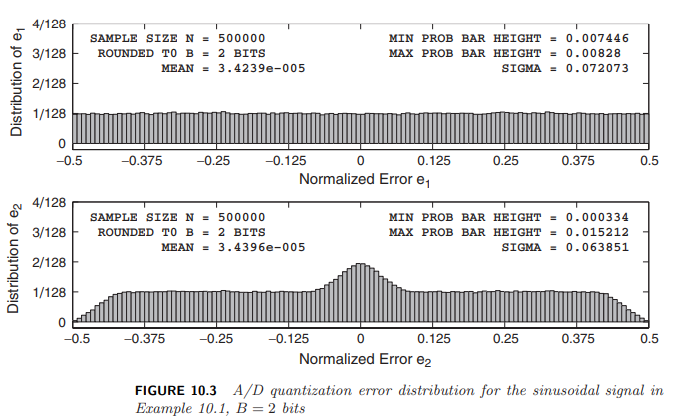
\includegraphics[width=1\linewidth]{QuantError1.png}
\end{figure}
To validate the model assumptions, we consider the following two examples. In the first example, an aperiodic sinusoidal sequence is quantized
to B bits, and in the second example, a random sequence is quantized to B
bits. The resulting quantization errors are analyzed for their distribution
properties and for their sample independence for various values of B. \\
\vspace{1em}
Let $x(n) = \frac{1}{3} {(\sin(n/11) + \sin(n/31) + \cos(n/67))}$. This sequence is not periodic, and hence its samples never repeat using infinite-precision representation.
However, since the sequence is of sinusoidal nature, its continuous envelope is
periodic and the samples are continuously distributed over the fundamental
period of this envelope. Determine the error distributions for B = 2 and 6 bits
\\
\vspace{1em}
To minimize statistical variations, the sample size must be large. We choose
500,000 samples. The following MATLAB script computes the distributions for
B = 2 bits.
\begin{lstlisting}
 clear; close all;
% Example parameters
B = 2; N = 500000; n = [1:N];
xn = (1/3)*(sin(n/11)+sin(n/31)+cos(n/67)); clear n;
% Quantization error analysis
[H1,H2,Q, estat]] = StatModelR(xn,B,N); % Compute histograms
H1max = max(H1); H1min = min(H1); % Max and Min of H1
H2max = max(H2); H2min = min(H2); % Max and Min of H2
\end{lstlisting}
The plots of the resulting histogram are shown in Figure 10.5. The corresponding plots for B = 6 bits are shown in Figure 10.6. From these plots, we observe
that even for B = 2 bits the quantization error samples are independent and
uniformly distributed.
\begin{figure}[H]
    \centering
    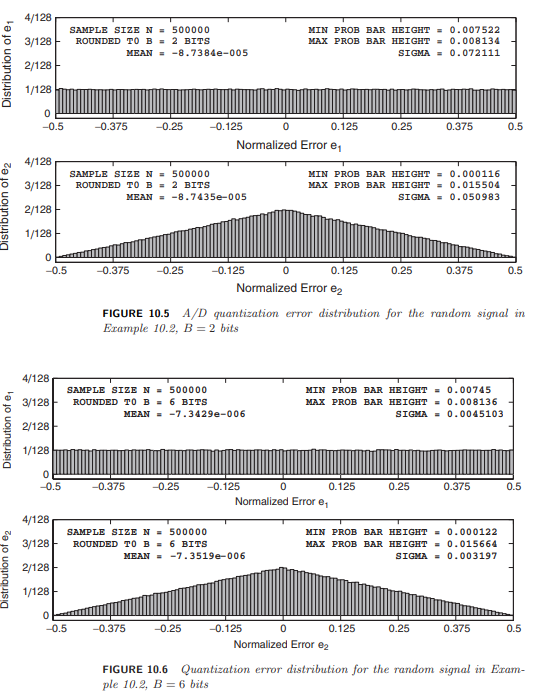
\includegraphics[width=1\linewidth]{QuantError2.png}
\end{figure}
\subsubsection{Intro to A/D Quantization Noise Through Digital Filters}
Let a digital filter be described by the impulse response, h(n), or the frequency response $H(e^{jw})$. When a quantized input, Q[x(n)] = x(n) + e(n) is applied to this system, we can determine the effects of the error sequence e(n) on the filter output as it propagates through the filter, assuming infinite-precision arithmetic implementation in the filter. We are generally
interested in the mean and variance of this output-noise sequence, which
we can obtain using linear system theory concepts. Details of these results
are given in Section 13.5.

\newpage
\section{Linear Algebra (unfinished)}
\subsection{Symbols}
\begin{tabular}{|c|c|}
\hline
\textbf{Symbol} & \textbf{Meaning}  \\
\hline
$\varnothing$ & Empty set \\
\hline
$\in$ & Member symbol \\
\hline
$\subseteq$ & Subset symbol \\
\hline
$\subset$ & Proper subset symbol \\
\hline
$\cap$ & Intersection symbol \\
\hline
$\cup$ & Union symbol \\
\hline
$\otimes$ & Tensor symbol \\
\hline
$\oplus$ & Direct sum symbol \\
\hline
$\approx$ & Approximate equality sign \\
\hline
$|A|$ & determinant of matrix A \\
\hline
$||u||$ & Norm of vector u \\
\hline
$||u||_p$ & p-norm of vector u \\
\hline
$A_{cof}$ & Cofactor matrix of A \\
\hline
$adjA$ & Adjoint of matrix A \\
\hline
$A^*$ & Conjugate (Hermitian) transpose of matrix A \\
\hline
$A^T$ & Transpose of matrix A \\
\hline
$C(A)$ & Column space of matrix A \\
\hline
$cond(A)$ & Condition number of matrix A \\
\hline
$\bar{z}$ & Complex conjugate of z \\
\hline
$det A$ & Determinant of A \\
\hline
$domain(T)$ & Domain of operator T \\
\hline
$diag\lambda_1...\lambda_n$ & Diagonal matrix with $\lambda_1...\lambda_n$ along diagonal\\
\hline
$\epsilon_\lambda$ & Eigenspace \\
\hline
$H_v$ & Householder matrix \\
\hline
$I,I_n$ & Identity matrix n x n identity \\
\hline
$id_V$ & Identity function for V \\
\hline
$ker(T)$ & Kernel of operator T \\
\hline
$M_{ij}$ & Minor of A \\
\hline
$\Null(A)$ & Null space of matrix A \\
\hline
$\rho(A)$ & Spectral radius of A \\
\hline
$T_A$ & Matrix operator associated with A \\
\hline
$R(\theta)$ & Rotation matrix \\
\hline


\end{tabular}

\newpage
\section{Statistics Review}
\subsection{Basics}
Mean: $\mu$ - Also know as the expected value E(X), X is a weighted average of the possible values of
X, with weights equal to the probabilities \\
\vspace{1em}
Variance: $\sigma^2 = V(x) = E(x-\mu)^2$ - is a measure of dispersion or scatter in the possible
values for X. \\
\vspace{1em}
Standard Deviation: $\sqrt{\sigma^2}$ \\
\vspace{1em}
Continuous - Lasting over a length and is infinite in length \\
\vspace{1em}
Discrete - Consists of many points which is sometimes infinite but countable \\
\vspace{1em}
Joint probability mass function of the discrete random variables X and Y,
denoted as $f_{XY}(x,y)$, satisfies
$f_{XY}(x,y) = P(X=x,Y=y), \space \space f_{XY}(x,y) \geq 0, \space \space \sum_x\sum_yf_{XY}(x,y)=1$ (probability X = x AND Y = y)
\subsection{Cross-Correlation \& Autocorrelation Sequences}
Having the two signal sequences, x(n), which is called the reference signal or
transmitted signal, and y(n), the received signal, the problem in radar and sonar
detection is to compare y(n) and x(n) to determine if a target is present and, if so,
to determine the time delay D and compute the distance to the target. In practice,
the signal x(n - D) is heavily corrupted by the additive noise to the point where
a visual inspection of y(n) does not reveal the presence or absence of the desired
signal reflected from the target. Correlation provides us with a means for extracting
this important information from y(n). \\
\vspace{1em}
Suppose that we have two real signal sequences x(n) and y(n) each of which has
finite energy. The cross-correlation of x (n) and y (n) is a sequence $r_{xy}(l)$. is defined as
\begin{equation}
r_{xy}(l) = \sum_{n=-\infty}^{\infty}x(n+1)y(n), \space l = 0 ,\pm 1, \pm 2
\end{equation}
The index l is the (time) shift (or lag) parameter and the subscripts xy on the cross-correlation sequence  indicate the sequences being correlated. The order of
the subscripts, with x preceding y, indicates the direction in which one sequence
is shifted, relative to the other.
\begin{center}
Determine the crosscorrelation sequence $r_{xy} (l)$ of the sequences   \\
\vspace{1em}

x(n) = ${0, 0, 2, -1, 3, 7, \underset{\uparrow}{1}, 2, -3, 0, 0,...}$ \\
\vspace{1em}
y(n) = ${..., 0, 0, 1, -1, 2, -2, \underset{\uparrow}{4}, 1, -2, 5, 0, 0,...}$
\end{center}
Computing $r_{xy}(l)$ for l = 0
\begin{center}
    $r_{xy}(0) = \sum_{n=-\infty}^{\infty}x(n)y(n)$
\end{center}
The product sequence $v_0(n) = x(n)y(n)$ is
\begin{center}
    $v_0(n) = {..., 0, 0, 2, 1, 6, -14, \underset{\uparrow}{4}, 2, 6, 0, 0,...}$
\end{center}
and hence the sum over all values of n is
\begin{center}
    $r_{xy}(0) =7$
\end{center}
For $l > 0$, we simply shift y(n) to the right relative to x(n) by l units, compute the product
sequence $v_l(n) = x(n)y(n - l)$, and finally, sum over all values of the product sequence. Thus
we obtain
\begin{center}
    $r_{xy} (1) = 13, r_{xy} (2) = -18, r_{xy} (3) = 16, r_{xy} (4) = -7$ \\
    $r_{xy} (5) = 5, r_{xy} (6) = -3, r_{xy} (l) = 0, l \geq 7$
\end{center}
For l < 0, we shift y(n) to the left relative to x(n) by l units, compute the product
sequence $v_l(n) = x(n)y(n - l)$, and sum over all values of the product sequence. Thus we
obtain the values of the crosscorrelation sequence
\begin{center}
    $r_{xy} (-1) = 0, r_{xy} (-2) = 33, r_{xy} (-3) = -14, r_{xy} (-4) = 36$ \\
    $r_{xy} (-5) = 19, r_{xy} (-6) = -9, r_{xy} (-7) = 10,r_{xy} (l) = 0, l \leq -8$
\end{center}
Therefore, the crosscorrelation sequence of x(n) and y(n) is
\begin{center}
    $r_{xy}(l) = {10, -9, 19, 36, -14, 33, 0, \underset{\uparrow}{7}, 13, -18, 16, -7, 5, -3}$
\end{center}
We note that the absence of folding $y(-l)$ makes crosscorrelation a noncommutative
operation. In the special case where y(n) = x(n), we have the autocorrelation of
x(n), which is defined as the sequence
\begin{equation}
    r_{xx}(l) = \sum_{n=-\infty}^{\infty}x(n)x(n-l)
\end{equation}
or, equivalently, as
\begin{equation}
    r_{xx}(l) = \sum_{n=-\infty}^{\infty}x(n+l)x(n)
\end{equation}
In dealing with finite-duration sequences, it is customary to express the autocorrelation and crosscorrelation in terms of the finite limits on the summation. In
particular, if x(n) and y(n) are causal sequences of length N [i.e., x(n) = y(n) = 0
expressed as
\begin{equation}
    r_{xy}(l) = \sum_{n=l}^{N-|k|-1}x(n)y(n-l)
\end{equation}
and
\begin{equation}
    r_{xx}(l) = \sum_{n=l}^{N-|k|-1}x(n)x(n-l)
\end{equation}
$k = 0$ for $l \geq 0$, $k = l$ for $l < 0$.
\subsection{Covariance}
The covariance is defined for both continuous and discrete random variables by the same formula. The covariance between the random variables X and Y, denoted as cov(X,Y) or $\sigma_{XY}$ is 
\begin{equation}
\sigma_{XY}=E[(X-\mu_X)(Y-\mu_Y)]=E(XY)-\mu_x\mu_Y
\end{equation}
Covariance is a measure of linear relationship between the random variables. If the relationship between the random variables is nonlinear, the covariance might not be sensitive to
the relationship
\begin{figure}
    \centering
    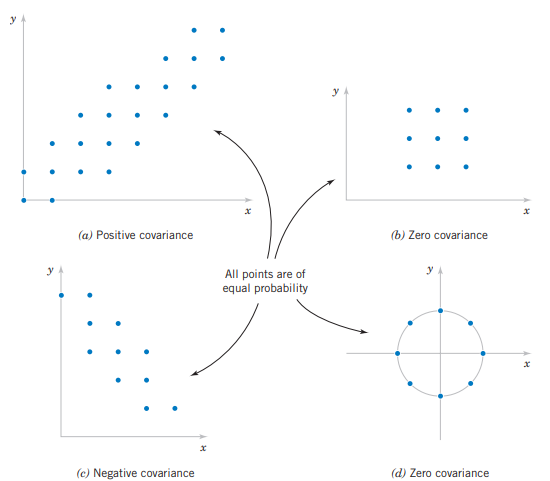
\includegraphics[width=1\linewidth]{Covariance.png}
\end{figure}
\subsection{Point Estimation}
\subsubsection{Mean Squared Error of an Estimator}
The mean squared error of an estimator of the parameter $\Theta$ is defined as
\begin{equation}
    MSE(\Theta) = E(\Theta-\theta)^2
\end{equation}

\newpage
\section{Random Processes}
The main focus in the first ten chapters was on characterizing, processing, and filtering deterministic signals—that is, signals defined using exact
mathematical expressions or through their Fourier spectra. In the real
world, there are signals that cannot be completely described as deterministic or that have random fluctuations (or variations) around known
waveforms. Speech signals, audio signals, video signals, and so on, fall
under the first category, while noisy signals, received radar signals, and
communication signals fall under the second category. Such signals are
known as random processes or random signals and can be thought of as a
collection or ensemble of sample signals with associated probabilistic description. Therefore, we need a statistical approach to characterize them
and to process them.
In Chapters 14 and 15, we will consider the processing of random
signals. Although linear filtering of a sample waveform from the ensemble
of the process is akin to convolution operation in the time domain or
filtering in the frequency domain, the emphasis will be on estimating
parameters from observations, detecting signals in noisy environments
and designing optimal filters for satisfying a given optimality criteria.
In this chapter, we provide an overview of various analytical concepts
to define randomness of measurements or waveform variations and provide sound techniques to calculate the response of linear filters to random
signals. We begin with the relevant probability theory of random variables by defining probability functions and statistical averages, and continue with pairs of random variables. We extend these concepts to random signals, describe them in terms of second-order statistics, and then delve
into stationary and ergodic processes, correlations, and power spectra.
We also show how this theory can be applied to processing of random signals through an LTI system using both the time and frequency domains.
Finally, we discuss a few representative random processes, including Gaussian, Markov, white noise, and filtered noise processes.

\subsection{Motivation}
When we make measurements of certain variables over a collection of
objects—for example, height in meters or weight in kilograms of a
population—we obtain numbers that fluctuate over a range of values.
Such measurements are called random measurements, the act of measurement is called a random experiment, and the variables are termed random
variables. Even if we consider repeating the same random experiment—
say, rolling a six-sided die—again and again, the outcomes vary and
cannot be predicted. In the context of signal processing, the value of a
noisy signal at each instant cannot be determined precisely and hence
must be considered as a random value.
Even though the numerical outcomes of these random experiments
vary widely every time we repeat them, there appears to be some pattern
of their relative likelihood of obtaining these values. Such patterns can be
understood and quantified using probability measure. For example, if we
toss a fair coin, we will not know if the outcome of the toss is a head or
a tail. But if we repeat this toss a large number of times, we will observe
that the total number of head/tail outcomes are approximately equal.

\subsection{Random Variable}
Consider a random variable under measurement such as a noisy voltage
source. We will use capital letters such as X to denote a random variable
and lowercase x to denote its measured value. Thus x is a value on a real
line R. We divide this line into small intervals of length $\Delta x$ and count the
number of voltage values, say, $N_x$ that fall into $\Delta x$ at each x. If N is the
total number of times we measure the random voltage X, then $\frac{N_x}{N}$ is
the approximate probability of observing voltage value x and $\frac{N_x/N}{\Delta x}$
is approximately the probability density of the random variable X at x. We
will denote this probability density function (pdf) as $f_X(x)$ and formally
define it by
\begin{equation}
f_X(x) = \lim_{\substack{\Delta x \to 0 \\ N \to \infty}} \left( \frac{N_x}{N \Delta x} \right)
\end{equation}
The probability that the random voltage X takes values over the range $x_1 < X < x_2$ is given by integrating $f_X(x)$dx over the interval, or 
\begin{equation}
Pr\{x_1 < X < x_2 \} = \int_{x_1}^{x_2}f_X(x)dx
\end{equation}
The pdf has to satisfy important properties for it to be a valid function.
It cannot be negative or imaginary, and every measurement must yield
some real value signifying
\begin{equation}
\int_{-\infty}^{\infty}f_X(x)dx=1
\end{equation}
The formulas for CDF and Discrete Random Var will not be provided for summary of this sectIon, just google them. \\
\vspace{1em}
MATLAB provides a function, Nx =
histc(x,edges), that provides counts in Nx, given observed values x and
bin edges. Using this function, we can design a MATLAB function, which
we will call pdf1, that computes the pdf as a normalized histogram from
the observed values.
\begin{lstlisting}
function [Px,xc] = pdf1(x,xmin,xmax,M)
% pdf1: Normalized Histogram as 1-D Probability Density
% Function (pdf)
% [Px,xc] = pdf1(x,xmin,xmax,M)
% Px: normalized histogram over the range [xmin, xmax]
% xc: histogram bin centers
% x: data (observation) values
% xmin: minimun range value
% xmax: maximum range value
% M: number of bins
N = length(x); % Observation count
edges = linspace(xmin,xmax,M); % Histogram boundaries
Dx = (xmax-xmin)/(M-1); % Delta_x
xc = [xmin,edges(1:M-1)+Dx/2,xmax]; % Bin centers
edges = [-inf,edges,inf]; % Augment boundaries
Nx = histc(x,edges); Nx = Nx(1:end-1); % Histogram
Px = Nx/(N*Dx); % Normalized Histogram
end
\end{lstlisting}
Consider the signal 
\begin{center}
$x(t) = \sin(2\pi t), 0 \leq t \leq 1$
\end{center}
We will take large samples of this waveform and consider them as the observed
values for computing and plotting the normalized histogram. The following
MATLAB script illustrates the approach.
\begin{lstlisting}
 N = 1000000; % Number of observations
 n = 0:1:N; % Time index
 x = sin(2*pi*n/N); % Observations
 [Px,xc] = pdf1(x,-1,1,100); % Normalized Histogram
 plot(xc(2:end-1),Px(2:end-1),'linewidth',1);
 axis([-1.1,1.1,0,3.5]);
 xlabel('Range of {\itx}','fontsize',9);
 ylabel('Relative Histogram','fontsize',9);
 set(gca,'xtick',[-1,0,1],'ytick',[0,1/pi,1,2,3,4]); grid;
 title('Approximation of pdf by Normalized Histogram',...
'fontsize',10,'fontweight','bold');
\end{lstlisting}
\begin{figure}[H]
    \centering
    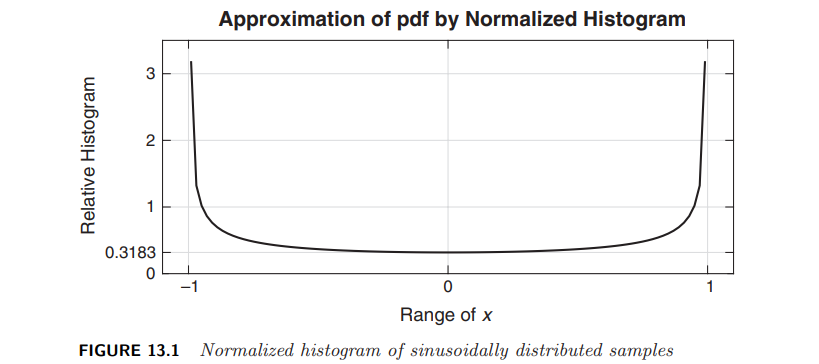
\includegraphics[width=1\linewidth]{pdfX.png}
\end{figure}
MATLAB provides the function x=rand
(N,1), which generates a column vector containing N standard uniform random numbers each of which is uniform over the interval [0, 1]. These
numbers are independent of each other; that is, generation of each one of
them does not affect the occurrence of any other.
\begin{lstlisting}
x = (b-a)*rand(N,1)+a;
\end{lstlisting}
\begin{figure}[H]
    \centering
    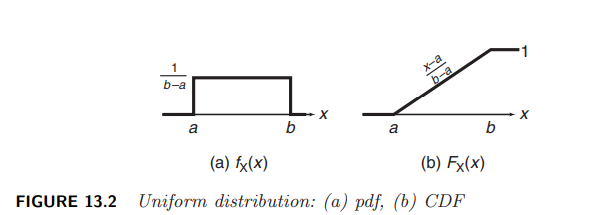
\includegraphics[width=0.5\linewidth]{Uniform.png}
\end{figure}
\subsubsection{Gaussian Distribution}
This is a very popular distribution model in many applications. MATLAB provides the function x =
randn(N,1), which generates a column vector containing N independent
and Normally distributed random numbers with mean 0 and variance 1.
To obtain arbitrary Gaussian distributed random numbers with mean $\mu$
and variance $\sigma^2$, we make a simple change of variable X = $\sigma$Y + $\mu$ where
Y is Normal:
\begin{lstlisting}
x = sigma*randn(N,1)+mu;
\end{lstlisting}
\begin{figure}[H]
    \centering
    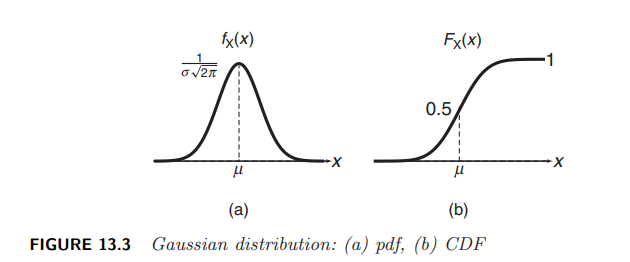
\includegraphics[width=0.5\linewidth]{Guassian.png}
\end{figure}
\subsubsection{Estimation of the mean of a random variable}
The built-in MATLAB function mean(X)
computes the average or mean value of the elements in the array X. If X is
a matrix, then mean(X) contains the mean value of each column of X. This
function implements the estimate of the mean value. Similarly, the var(X)
computes the variance of the values in X. \\
\vspace{1em}
The following MATLAB script shows the generation of random variables and
estimation of mean as well as its display from 10 samples.
\begin{lstlisting}
 a = 0; b = 2; % Uniform random variable parameters
 mu_X = (a+b)/2; % True mean value
 N = 10; % Number of values
 x = (b-a)*rand(N,1)+a; % Random data values
 mu_hat = mean(x); % Mean estimate
 disp(['True Mean value of X is: ',num2str(mu_X,2)]);
True Mean value of X is: 1
 disp([' Estimated Mean is: ',num2str(mu_hat,2)]);
Estimated Mean is: 0.94
\end{lstlisting}
The above script indicates that the estimated mean is very close to the true
mean even for 10 samples. The following script repeats the above experiment
100 times and computes as well as plots the results.
\begin{lstlisting}
 M = 100; % Number of experiments
 x = (b-a)*rand(N,M)+a; % M experiments, each N values
 mu_hat = mean(x); % Mean estimate of each column
 mean_muhat = mean(mu_hat); % Mean of the estimates
 var_muhat = var(mu_hat); % Variance of the estimates
 disp([' Mean value of the estimate is: ',...
num2str(mean_muhat,2)]);
Mean value of the estimate is: 1
 disp(['Estimated variance of the estimate is: ',...
num2str(var_muhat,2)]);
Variance of the estimate is: 0.034
 disp([' True variance of the estimate is: ',...
num2str(var_mutrue,2)]);
True variance of the estimate is: 0.033
% Plotting commands follow
\end{lstlisting}
\begin{figure}[H]
    \centering
    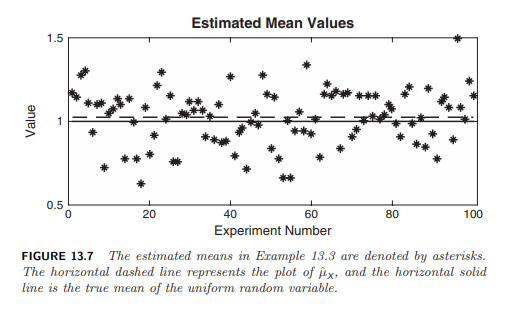
\includegraphics[width=0.5\linewidth]{MeanEstimate.png}
\end{figure} 
\subsection{Random Signals}
A random signal or process can be thought of as a collection of waveforms
(or time-varying values) with some assigned probability. Similarly, we can
think of the value of a random signal at each time instant as a random
variable with an assigned pdf. Thus a random signal is a collection of
random variables in the temporal space as well as a collection of sample waveforms in the ensemble space. This understanding is crucial in
dealing with its probabilistic (or statistical) description as well as for its
processing through linear systems.
A random process can be continuous in time (random signals) or discrete in time (random sequences). We will mostly discuss random signals,
but the derived results will also apply to random sequences with obvious
modifications that we will also state. In keeping with our random variable
terminology, we will denote a random signal by X(t) and its realization or
sample waveform by x(t). Thus we have a new temporal variable in our
random object.
If a time instance t is fixed (i.e., when we assign a known value), then
X(t) is a random variable
\subsubsection{Strict-Sense Stationary}
In this type of stationarity, all orders of joint density functions or,
alternatively, all orders of joint moments are time invariant, that is, the
first-order densities are independent of time
\begin{equation}
f_X(x;t)=f_X(x)
\end{equation}
and the joint densities are independent of time t but depend only on the
relative interval $\tau$ between the two time instances
\begin{equation}
f_X(x_1,x_2;t_1=t+\tau,t_2=t)=f_X(x_1,x_2;\tau=t_1-t_2)
\end{equation}
and so on, for all orders. This also means that
\begin{center}
\begin{equation}
\mu_X(t) = \mu_X, E[X^2(t)]=\epsilon_X(2)
\end{equation}
\begin{equation}
R_{XX}(t_1,t_2)=R_{XX}(t_1-t_2)
\end{equation}
\begin{equation}
C_{XX}(t_1,t_2)=C_{XX}(t_1-t_2)    
\end{equation}
\end{center}
\subsubsection{Wide-Sense Stationarity}
In many practical applications, we need or use only up to second-order
statistical quantities of a random signal. Therefore, why not require timeinvariance only for the first two orders of moments? This leads to a weaker
but workable form of stationarity called wide-sense stationarity, or WSS.
We will say that a random signal X(t) is WSS if it satisfies the following
three conditions:
\begin{equation}
E[X^2(t)]= \zeta_x(2) < \infty \space \space \text{(finite average power)}
\end{equation}
\begin{equation}
\mu_X(t) = \mu_X \space \space \text{(a constant)}
\end{equation}
\begin{equation}
R_{XX}(t+\tau,t) = R_{XX}(\tau) \space \space \text{(function of $\tau$ only)}
\end{equation}
The variable $\tau$ is called the lag time variable since the random variable
X(t) lags X(t +  $\tau$ ) in time by  $\tau$ seconds. Clearly, the autocovariance function $C_{XX}(t, t + \tau )$ also exhibits a similar time-invariance as in
\begin{equation}
C_{XX}(t+\tau,t) = C_{XX}(\tau)
\end{equation}
Note that a random process in is nonstationary if
both its first- and second-order moments are functions of time, whereas
a random process in is WSS if its mean is constant
and its autocorrelation function depends only on $(t_1 - t_2)$, which, from
(13.107), can be written as 
\begin{equation}
R_{XX}(t+\tau,t) = R_{XX}(\tau) = \frac{1}{4}\cos(\Omega_0\tau)    
\end{equation}
In the rest of the chapter, we will mostly deal with WSS random
signals. Therefore, if we state that a random signal has a constant mean
and an autocorrelation function that depends on a single time variable,
then the reader can infer that the signal is WSS.
Finally, if X(t) and Y(t) are jointly WSS, then their cross-correlation
and cross-covariance functions depend only on the lag variable $\tau$ ; that is,
\begin{equation}
R_{XY}(t+\tau,t)= R_{XY}(\tau) \space \space \text{  and } \space \space C_{XY}(t+\tau,t) = C_{XY}(\tau)
\end{equation}
he autocorrelation sequence (ACRS) of a wide-sense stationary process is
\begin{equation}
r_{xx}(\tau)=c_{xx}(\tau)+m^2_x
\end{equation}
Take the equation 
\begin{center}
$x[n] = A\cos(\omega n + \phi)$, $\phi =(0,2\pi)$
\end{center}
If A and $\omega$ are fixed quantities and $\phi$ is a uniformly distributed, the stochastic process is wide-sense stationary.

\subsubsection{Cross-Correlation}
Cross-correlation measures the similarity between two signals as one is shifted (lagged) over the other. It tells you how well one signal matches a time-shifted version of another.
\begin{equation}
r_{xy}[l]=\sum_{n}x[n]y[n+l]
\end{equation}
l is the lag (positive or negative shift) \\
$r_{xy}[l]$ is large when y[n+l] looks like x[n] \\
\vspace{1em}
MATLAB Implementation 
\begin{lstlisting}
[Rxy,lags]=xcorr(x,y,maxlags,'option')
\end{lstlisting}
that estimates cross-correlation values Rxy at lag indices lags between
two data vectors x and y. The correlation values are computed up to
the maxlag index using four option cases: 'none' (default), 'biased',
'unbiased', and 'coeff', which are described below. It also computes
the autocorrelation values using the invocation. \\
\vspace{1em}
\subsubsection{Properties of correlation and covariance sequences}


Consider a noisy signal that consists of a churp. If we want to discern when the chirp occurs, we take the cross-correlation using MATLAB.
\begin{lstlisting}
load chirp
template = y;

mixed = template + 0.5 * randn(size(template));  % noisy mix

[c, lags] = xcorr(mixed, template);
[~, idx] = max(abs(c));
estimated_delay = lags(idx);    
\end{lstlisting}
\subsection{Power Spectral Density}
Power distribution can be gleaned from the analysis of
the pairs of random variables and, in particular, from the autocorrelation
function. The result is a new term called power spectral density, or PSD.
To develop this result, we will need the use of Fourier analysis. We
studied and used Fourier transforms of continuous- and discrete-time
signals in previous chapters where signals were mostly deterministic and
satisfied certain convergence conditions such as finite power or absolute
integrability \\
\vspace{1em}
Is denoted as $S_{XX}(w)$
\subsubsection{MATLAB implementation}
The SP Toolbox provides several functions, such as pwelch and cpsd, to estimate PSD and CSD functions,
respectively, from data vectors. These functions use techniques from spectral estimation theory, a topic that is beyond the scope of this book. Since
we have used the xcorr function to estimate autocorrelation lag values,
we will compute the FFT of a large number of suitably zero-padded autocorrelations as a preferred implementation of the PSD estimate. Since the autocorrelation values being transformed are still finite
in number (and not infinite as the theory requires), this computation
amounts to windowing the original autocorrelation sequence by a rectangular window. This may result in some of the computed PSD values
becoming negative, which violates one of the PSD properties. Therefore,
we will use a window function whose DTFT is always non-negative. Such
windows are known as lag windows, and one such window is the Bartlett
(or triangular) window.
\begin{lstlisting}
function [Sx,omega] = PSD(Rx,maxlag,Nfft)
%PSD Computation of PSD using Autocorrelation Lags
% [Sx,omega] = PSD(Rx,lags,Nfft)
% Sx: Computed PSD values
% omega: digital frequency array in pi units from -1 to 1
% Rx: autocorrelations from -maxlag to +maxlag
% maxlag: maximum lag index (must be >= 10)
% Nfft: FFT size (must be >= 512)
Nfft2 = Nfft/2;
M = 2*maxlag+1; % Bartlett window length
Rx = bartlett(M).*Rx(:); % Windowed autocorrelations
Rxzp = [zeros(Nfft2-maxlag,1);Rx;zeros(Nfft2-maxlag-1,1)];
Rxzp = ifftshift(Rxzp); %Zero-padding and circular shifting
Sx = fftshift(real(fft(Rxzp))); % PSD
Sx = [Sx;Sx(1)]; % Circular shifting
omega = linspace(-1,1,Nfft+1); % Frequencies in units of pi
end
\end{lstlisting}
We will demonstrate the use of the PSD function in the following MATLAB
script.
\begin{lstlisting}
 load x; maxlag = 10; %Load random sequence data
 [Rx,lags] = xcorr(x,maxlag,'coeff'); % Compute ACRS
 [Sx,omega] = PSD(Rx,maxlag,512); % Compute PSD
 % Plotting commands follow
\end{lstlisting}
\begin{figure}[H]
    \centering
    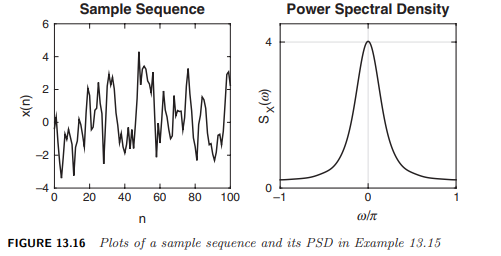
\includegraphics[width=1\linewidth]{PSD.png}
\end{figure}
The plot shows how power (energy) is distributed across frequencies.

\subsection{Useful Random Processes (Most relevant of this section, unfinished)}
\subsubsection{Guassian Process}
Another
crucial reason why Gaussian distribution is necessary can be found in the
ever-present thermal noise that is produced by the random movement of
agitated electrons in electrical devices. To understand this Gaussian behavior, consider a resistor. The free
electrons in a resistor move as a result of thermal agitation. This movement is random and can be in any direction. However, their velocity is
proportional to the ambient temperature; the higher the temperature,
the higher the velocity. This movement generates a current with a random value. We can model each electron as a tiny current source whose
current is a random variable with positive or negative values. The total
current generated (which is the thermal noise) is the sum of all these current sources. Quantum mechanics suggests that the electron movements
(i.e., current sources) are statistically independent. Thus the thermal noise
is a sum of a large number of IID random sources. Using the central limit
theorem, we conclude that this total current has a Gaussian distribution.


\subsubsection{White Noise Process}
This is an idealization of the thermal noise generated in electronic devices that helps in analysis immensely. Recall the discussion leading up to
the Gaussian process in the previous section. Using quantum mechanical analysis, it can be shown that the thermal noise is a zero-mean stationary
process.
\begin{figure}[H]
    \centering
    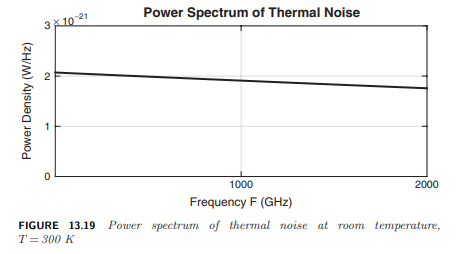
\includegraphics[width=0.5\linewidth]{ThermalNoise.png}
\end{figure}
In a similar fashion, a discrete-time white noise process W(n) is defined
as a zero-mean stationary random sequence. In addition, if W(n) is also Gaussian at each n, then it is termed a WGN
process, which is also an independent process. Sample sequences for independent WN processes are easy to generate in MATLAB using the randn
or rand functions. For example,
\begin{lstlisting}
Wn = randn(N,1);
\end{lstlisting}
generates N samples of unit variance WGN process, while 
\begin{lstlisting}
Wn = rand(N,1);
\end{lstlisting}
generates N samples of unit variance independent WN process. \\
\vspace{1em}
Generate 10,000 samples of a WGN random process with variance $\sigma^2_W=4$
Numerically estimate autocorrelation lag values $R_{WW}(\ell)$, $-20 \leq \ell \leq 20$ and use
these to compute the PSD $S_{WW}(2\pi f)$. Repeat this procedure over 100 sample
sequences to reduce variability of estimates and average $R_{WW}(\ell)$ and $S_{WW}(2\pi f)$
over these sample functions and plot the resulting quantities. \\
\vspace{1em}
We will use the randn function to generate WGN samples, the xcorr function to
estimate autocorrelation lag values, and the PSD function to compute the PSD.
These steps and averaging operations are illustrated in the following MATLAB
script.
\begin{lstlisting}
> M = 100; % Number of sample sequences to average over
 N = 10000; % Number of samples in each sequence
 varW = 4; % Variance of the process
 sigW = sqrt(varW); % Standard deviation
 maxlag = 20; % Maximum number of lag values
 Nfft = 1024; Nfft2 = Nfft/2; % FFT size
 Rwsum = zeros(2*maxlag+1,1)'; % Rw initialization
 Swsum = zeros(Nfft+1,1); % Sw initialization
 ell = -maxlag:maxlag; % Lag indices for plotting
 f = linspace(-0.5,0.5,Nfft+1); % Frequency grid for plotting
 % Loop over M Sample Sequences
 for k = 1:M
 % Generate 10000 samples of WGN Process
 wn = sigW*randn(N,1)';
 % Compute ACRS
 [Rw,lags] = xcorr(wn, maxlag,'unbiased');
 Rwsum = Rw+Rwsum; % Sum autocorrelations
 Sw = PSD(Rw',maxlag,Nfft); % Compute PSD
 Swsum = Sw+Swsum; % Sum PSD values
 end
 Rw = Rwsum/M; % Average autocorrelations
 Sw = Swsum /M; % Average PSD
 % Plotting commands follow
\end{lstlisting}
\begin{figure}
    \centering
    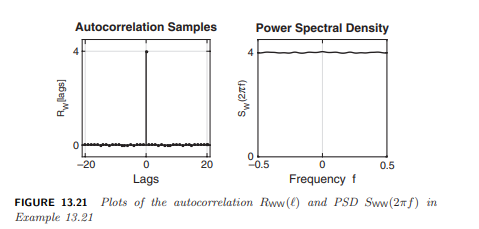
\includegraphics[width=0.75\linewidth]{WGN.png}
\end{figure}
\subsubsection{Markov Process}
In some applications, it is advantageous to model a random process whose
future values depend only on the present value. This reduces storage as
well as processing complexities. Such a process is called a Markov process,
and it is a process whose past has no influence on the future given that its
present is specified; that is, $t_n>t_{n-1}$  then the conditional distribution
of a Markov process X(t) based on the infinite past. \\
\vspace{1em}
Generate 10,000 samples of a Gauss–Markov process X(n) that has correlation
coefficient $\rho$ = 0.7 and average power of 100 watts. \\
\vspace{1em}
We will use (13.220) with $\rho$ = 0.7 to generate samples of X(n) from W(n). To
generate the WGN W(n), we will need its variance $\sigma^2_W$
W. Following the steps used
in Example 13.14, we can show that the autocorrelation of X(n) in (13.220) is
given by
\begin{equation}
R_{XX}(\ell) = (\frac{\sigma^2_W}{1-\rho^2})\rho^{|\ell|}
\end{equation}
\begin{equation}
R_{XX}[0]=\frac{\sigma^2_W}{0.51}
\end{equation}
Hence for $R_{XX}[0]$ = 100, we obtain {$\sigma^2_W = 51$}. Now we will generate samples of
W(n) using the randn function and filter those samples using $X(n) = \rho X(n-1) +W(n)$to obtain
samples of X(n). 
\begin{lstlisting}
 N = 10000; varW = 51;
 wn = sqrt(varW)*randn(N,1);
 rho = 0.7; b = 1; a = [1,-rho];
 xn = filter(b,a,wn);
\end{lstlisting}
\subsubsection{Filter Noise Process}
Even if we model the thermal noise as a white noise process at the input
of a communication receiver system, it gets processed, or, more correctly,
filtered, by subsequent stages of operations in the receiver. At each stage,
a correlated noise process is generated, known as a color noise process, or
colored process for short. If the frequency response function of the receiver is $H(j\Omega)$ and the input is WGN W(t) with PSD $S_{WW}(\Omega)=N_0/(4\pi)$ then the colored process X(t) is also zero mean. Generally, the stages in the receiver are bandpass systems, and hence
the filtered noise is a bandpass process. However, the information signals generally have lowpass power distribution. We now consider both
processes below. \\
\vspace{1em}
\textbf{Lowpass Process} \\
A random process X(t) is called lowpass if its power spectrum is large in
the vicinity of F = 0 Hz and small (approaching 0) at high frequencies.
In other words, a lowpass random process has most of its power concentrated at low frequencies. 
\begin{figure}
    \centering
    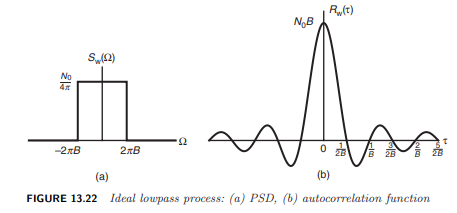
\includegraphics[width=1\linewidth]{LowPassProcess.png}
\end{figure}
Consider the problem of generating samples of a bandlimited lowpass process by
filtering a discrete-time WGN process through a properly designed IIR elliptic
filter that approximates the ideal lowpass filter. Obtain samples X(n) of a
lowpass process X(t) that is bandlimited to 3 KHz using a fifth-order elliptic
filter. Choose a sampling rate of 20 KHz. \\
\vspace{1em}
First, we will design a fifth-order elliptic filter by setting passband cutoff frequency to $\omega p$ = (3/20)2$\pi$ = 0.3$\pi$. To approximate the ideal lowpass filter, we
will choose passband ripple of 0.1 dB and stopband attenuation of 50 dB, which
are quite reasonable. Now using the ellip function, we obtain the required lowpass filter that can be used in filtering WGN samples to obtain samples of the
bandlimited lowpass process. The following MATLAB script gives all the necessary details
\begin{lstlisting}
M = 100; % Number of sample sequences to average over
N = 10000; % Number of samples in each sequence
varW = 4; % Variance of the input WGN process
sigW = sqrt(varW); % Standard deviation
maxlag = 50; % Maximum number of lag values
Nfft = 2048; Nfft2 = Nfft/2; % FFT size
Rxsum = zeros(2*maxlag+1,1)'; % Contains Autoc sum for averaging
Sxsum = zeros(Nfft+1,1); % Contains PSD sum for averaging
ell = -maxlag:maxlag; % Lag indices
f = linspace(-0.5,0.5,Nfft+1); % Frequency grid
% Approximation to Ideal LPF using Elliptic Filter
omp = 0.3; % Passband cutoff in pi units
Rp = 0.1; % Passband ripple in dB
As = 50; % Stopband attenuation in dB
Nellip = 5; % Order of the elliptic filter
[b,a] = ellip(Nellip,Rp,As,omp); % Elliptic filter coefficients
% Loop over M Sample Sequences
for k = 1:M
% Generate 10000 samples of WGN Process
wn = sigW*randn(N,1)';
xn = filter(b,a,wn); % Filtered WGN using lowpass filter
% Compute ACRS
[Rx,lags] = xcorr(xn, maxlag,'unbiased');
Rxsum = Rx+Rxsum;
Sx = PSD(Rx,maxlag,Nfft); % Compute PSD
Sxsum = Sx+Sxsum;
end
Rx = Rxsum/M;
Sx = Sxsum/M;
% Plotting commands follow
\end{lstlisting}
\begin{figure}[H]
    \centering
    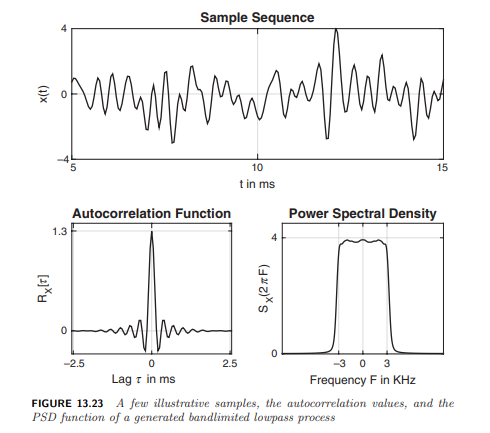
\includegraphics[width=1\linewidth]{PSDAutoWGNLow.png}
\end{figure}
Bandpass process \\
A random process is called a bandpass process if its power spectrum is
large in a band of frequencies centered in the neighborhood of a central
frequency $\pm F_0$ and relatively small outside of this band of frequencies. A
random process is called narrowband bandpass if its bandwidth B  $\ll$ $F_0$.
Let X(t) be the output of an ideal bandpass filter $H(j\Omega)$ whose input
is a WGN process W(t) with PSD $S_{WW}(\Omega)$ = $N_0/(4\pi)$. The ideal bandpass filter has a bandwidth of B Hz that is located at frequencies around
$F_0$ Hz. \\
\vspace{1em}
In this example, we will use the procedure of Example 13.23 to obtain samples
of an approximated bandlimited bandpass process. Generate samples X(n) of
a bandpass process X(t) that is bandlimited between 3 and 6 KHz using a
tenth-order bandpass elliptic filter. Choose sampling rate of 20 KHz. \\
\vspace{1em}
Again, we will first design a tenth-order elliptic filter by setting passband cutoff
frequencies to $\omega_{p_1}$ = (3/20)2$\pi$ = 0.3$\pi$ and $\omega_{p_2}$ = (6/20)2$\pi$ = 0.6$\pi$. To approximate the ideal bandpass filter, we will choose passband ripple of 0.1 dB
and stopband attenuation of 50 dB, which are quite reasonable. The stopband
cutoff frequencies will be set by the order of the filter. Now using the ellip
function, we obtain the required bandpass filter that can be used in filtering
WGN samples to obtain samples of the bandlimited bandpass process. The following MATLAB script gives all the necessary details. A representative segment
of the bandpass process, its autocorrelation, and the resulting PSD functions
are shown.
\begin{lstlisting}
M = 100; % Number of sample sequences to average over
N = 10000; % Number of samples in each sequence
varW = 1; % Variance of the input WGN process
sigW = sqrt(varW); % Standard deviation
maxlag = 50; % Maximum number of lag values
Nfft = 2048; Nfft2 = Nfft/2; % FFT size
Rxsum = zeros(2*maxlag+1,1)'; % Contains Autoc sum for averaging
Sxsum = zeros(Nfft+1,1); % Contains PSD sum for averaging
ell = -maxlag:maxlag; % Lag indices
f = linspace(-0.5,0.5,Nfft+1); % Frequencies in cycles/sam
Fs = 20; % Sampling rate in Khz
F = f*Fs; % Frequencies in KHz
% Approximation to ideal BPF using elliptic filter
omp1 = 0.3; % Lower Passband cutoff in pi units
omp2 = 0.6; % Upper Passband cutoff in pi units
Rp = 0.1; % Passband ripple in dB
As = 50; % Stopband attenuation in dB
Nellip = 5; % Order of the resulting elliptic filter is 2*N
[b,a] = ellip(Nellip,Rp,As,[omp1,omp2]); % Elliptic filter coefficients
% Loop over M sample sequences
for k = 1:M
% Generate 10000 samples of WGN Process
wn = sigW*randn(N,1)';
xn = filter(b,a,wn); % Filtered WGN using lowpass filter
% Compute ACRS
[Rx,lags] = xcorr(xn, maxlag,'unbiased');
Rxsum = Rx+Rxsum;
Sx = PSD(Rx,maxlag,Nfft); % Compute PSD
Sxsum = Sx+Sxsum;
end
Rx = Rxsum/M;
Sx = Sxsum/M;
% Plotting commands follow

\end{lstlisting}
\begin{figure}[H]
    \centering
    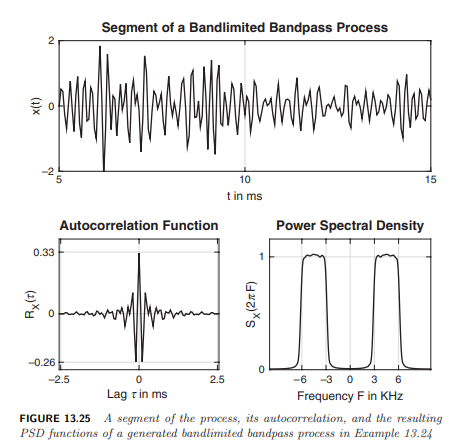
\includegraphics[width=1\linewidth]{AutoPSDBand.png}
\end{figure}
Bandpass processes are suitable for representing modulated signals.
In a communication system, the information-bearing signal is usually a
lowpass random process that modulates a carrier for transmission over a bandpass (narrowband) communication channel. Thus the modulated
signal is a bandpass random process.
A bandpass random process X(t) can be represented in terms of lowpass processes as
\begin{equation}
X(t) = X_c(t)\cos(2\pi F_0t) - X_s(t)\sin(2\pi F_0 t)
\end{equation}
where $X_c(t)$ and $X_s(t)$ are called the in-phase and quadrature components
of X(t). These random processes $X_c(t)$ and $X_s(t)$ are lowpass processes.
Furthermore, there is an important relationship among these X(t), $X_c(t)$,
and $X_s(t)$ processes, given below without proof: If X(t) is a zero-mean, stationary random process, then processes Xc(t)
and Xs(t) are also zero-mean, jointly stationary processes.
\begin{figure}[H]
    \centering
    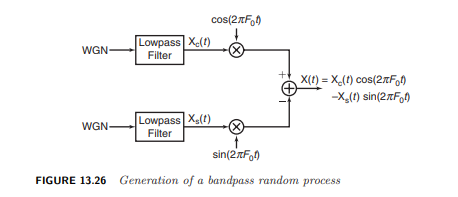
\includegraphics[width=1\linewidth]{BPGeneration.png}
\end{figure}
5 Generate samples of a Gaussian bandpass random process by first generating
samples of two statistically independent Gaussian random processes $X_c(t)$ and
$X_s(t)$ and then using these to modulate the quadrature carriers $\cos(2\pi F_0t)$ and
$\sin(2\pi F_0t)$ \\
\vspace{1em}
On a digital computer or in MATLAB, samples of the lowpass processes $X_c(t)$
and $X_s(t)$ are generated by filtering two independent Gaussian white noise sequences by two identical lowpass filters. Thus we obtain the samples $X_c(n)$ and
$X_s(n)$, corresponding to the sampled values of $X_c(t)$ and $X_s(t)$. Then $X_c(n)$ modulates the sampled carrier $\cos(2\pi F_0nT)$, and Xs(n) modulates the quadrature
carrier $\sin(2\pi F_0nT)$, where T is the appropriate sampling interval.
The MATLAB script for these computations is given below. For illustrative
purposes, we have selected the lowpass filter to have a system function
\begin{equation}
H(z) =\frac{1}{1-0.9z^{-1}}
\end{equation}
Also, we selected T = 0.001 sec or sampling rate of 1000 sam/sec and $F_0$ =
200 Hz. A representative segment of the bandpass process, its autocorrelation,
and the resulting PSD are shown 
\begin{lstlisting}
M = 100; % Number of sample sequences to average over
N = 10000; % Number of samples in each sample sequence
varW = 1; % Variance of the input WGN process
sigW = sqrt(varW); % Standard deviation
maxlag = 50; % Maximum number of lag values
Nfft = 2048; Nfft2 = Nfft/2; % FFT size
Rxsum = zeros(2*maxlag+1,1)'; % Contains Autoc sum for averaging
Sxsum = zeros(Nfft+1,1); % Contains PSD sum for averaging
ell = -maxlag:maxlag; % Lag indices
f = linspace(-0.5,0.5,Nfft+1); % Frequency grid
Fs = 1000; % Sampling rate in Khz
F = f*Fs; % Frequencies in KHz
F0 = 200; % Carrier frequency in Hz
T = 1/Fs; % Sampling interval
t = (0:N-1)*T; % Sampled time instances
% Lowpass filter for illustration
b = 1; a = [1,-0.9];
% Loop over M Sample Sequences
for k = 1:M
% Generate 10000 samples of WGN process
wcn = sigW*randn(N,1)'; % Input WGN for Xc(n)
wsn = sigW*randn(N,1)'; % Input WGN for Xs(n)
xcn = filter(b,a,wcn); % WGN -> lowpass filter -> Xc(n)
xsn = filter(b,a,wsn); % WGN -> lowpass filter -> Xs(n)
xn = xcn.*cos(2*pi*F0*t) - xsn.*sin(2*pi*F0*t); % BP process
% Compute ACRS
[Rx,lags] = xcorr(xn, maxlag,'unbiased');
Rxsum = Rx+Rxsum;
Sx = PSD(Rx,maxlag,Nfft); % Compute PSD
Sxsum = Sx+Sxsum;
end
Rx = Rxsum/M; Sx = Sxsum/M;
% Plotting commands follow
\end{lstlisting}
\begin{figure}[H]
    \centering
    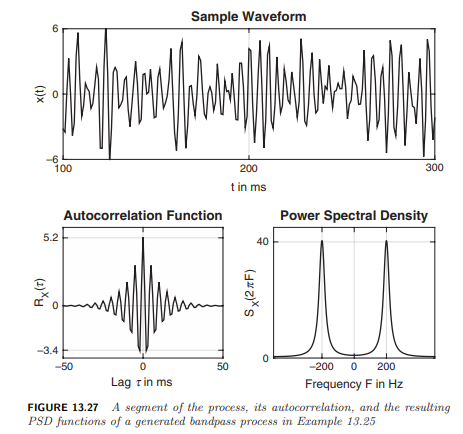
\includegraphics[width=1\linewidth]{BPProcessAutoPSD.png}
\end{figure}

\subsection{Causes of Noise in Systems}
1. Electromagnetic Interference (EMI) \\
Source: Nearby power lines, motors, Wi-Fi, switching power supplies, fluorescent lights, or other electronic devices.\\
2. Power Supply Noise\\
Source: Ripple from poorly regulated power supplies, switching transients from DC-DC converters. \\
Symptoms: You'll often see 60 Hz or 120 Hz hum (from AC line frequency or its harmonics) in analog circuits. \\
3. Thermal Noise (a.k.a. Johnson-Nyquist noise) \\
Source: Every resistor generates this due to random thermal motion of electrons. \\
 4. Crosstalk \\
Source: Signals from adjacent traces or wires coupling into each other. \\
5. Ground Loops \\
Source: Multiple paths to ground at different potentials, causing current to flow through unintended paths. \\
6. Quantization Noise (in DSP systems) \\
Source: Finite resolution of ADCs or digital systems. \\
7. Switching Noise \\
Source: Fast switching edges in digital systems (e.g., microcontrollers, FPGAs) that generate harmonics. \\
8. Layout-induced Noise \\
Source: Poor PCB layout, long signal return paths, missing ground planes.
\section{Linear Prediction and Optimum Linear Filters}
\subsection{Motivation}
You are working on a wearable biomedical device that records electrocardiogram (ECG) signals from a patient. However, the ECG is contaminated by 60 Hz power-line interference and sensor noise. The noise is uncorrelated with the clean ECG signal but measurable via a separate reference sensor.

Your objective is to recover the clean ECG signal as closely as possible. \\
\vspace{1em}
The measured ECG signal is:
\begin{center}
$x(n) = s(n) + v(n)$
\end{center}
where: \\
s(n): clean ECG signal (unknown, desired) \\
\vspace{1em}
v(n): additive noise (correlated with an auxiliary measurement) \\
\vspace{1em}
You are given a reference signal r(n), obtained from a nearby sensor, which captures the noise characteristics (e.g., 60 Hz + sensor noise), and is correlated with v(n) but uncorrelated with s(n). \\
\vspace{1em}
Design an optimal linear filter h(n), based on the reference r(n), such that: \\
\begin{center}
$$\hat{s}(n)=\sum_{k=0}^{M-1}h(k)x(n-k)$$
\end{center}
or, when using a reference signal:
\begin{center}
$$\bar{s}(n)=\sum_{k=0}^{M-1}h(k)r(n-k)$$
\end{center}
The design of filters to perform signal estimation is a problem that
frequently arises in the design of communication systems and control
systems, in geophysics, and in many other disciplines. In this chapter, we
treat the problem of optimum filter design from a statistical viewpoint.
The filters are constrained to be linear and the optimization criterion is
based on the minimization of the mean square error. As a consequence,
only the second-order statistics (autocorrelation and cross-correlation
functions) of a stationary process are required in the determination of
optimum filters.
Included in this treatment is the design of optimum filters for linear
prediction. Linear prediction is a particularly important topic in digital
signal processing, with applications in a variety of areas, such as speech
signal processing, image processing, and noise suppression in communication systems. 
\subsection{Summary of 14.1 (finish autocorrelation plots)}
In this section, we demonstrate that a wide-sense stationary random process may be represented as the output of a causal and causally invertible
linear system excited by a white noise process. The condition that the
system is causally invertible also allows us to represent the wide-sense
stationary random process by the output of the inverse system, which is
a white noise process Let us consider a wide-sense stationary process X(n) with autocorrelation sequence $R_{XX}(m)$ and power spectral density $S_{XX}(f)$, $|f| \leq \frac{1}{2}$. We
assume that $S_{XX}(f)$ is real and continuous for all $|f| \leq \frac{1}{2}$. The z-transform
of the autocorrelation sequence $R_{XX}(m)$ was termed the complex PSD
and is given by
\begin{equation}
S_{XX}(z) = \sum_{m=-\infty}^{\infty}R_{XX}(m)z^{-m}
\end{equation}
\begin{equation}
\log S_{XX}(z) = \sum_{m = -\infty}^{\infty}v(m)z^{-m}
\end{equation}
\begin{equation}
\log S_{XX}(f) = \log\sigma^2_W+\log H(f) + \log H^*(f)= \sum_{m=-\infty}^{\infty}v(m)e^{-j2\pi fm} 
\end{equation}
\begin{equation}
S_{XX}(f) = \sigma^2_W|H(f)|^2
\end{equation}
\begin{equation}
H(z) = \sum_{n=0}^{\infty}h(n)z^{-n}
\end{equation}
Note: $S_{XX}(f) = S_{XX}(2\pi f)$
\begin{figure}[H]
    \centering
    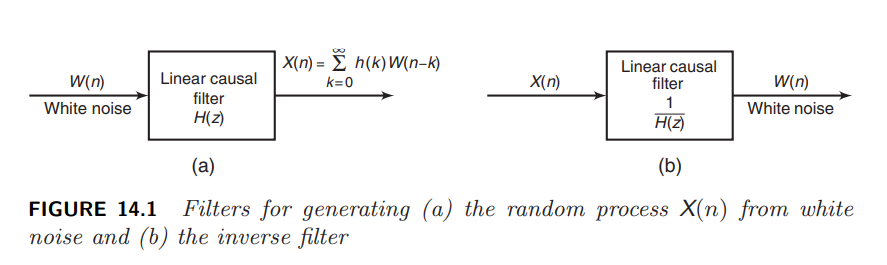
\includegraphics[width=1\linewidth]{LinearCasualFilterBlock.png}
\end{figure}
A linear casual filter transforms white noise into a stationary random process X(n) and the inverse of the linear casual filter transforms a random process into white noise, hence why the inverse of the linear casual filter is called a "noise whitening filter".
\subsection{Properties of the Linear Prediction-Error Filters }
Linear prediction-error filters possess several important properties, which
are described in this section. We begin by demonstrating that the forward
prediction-error filter is minimum phase. \\
\vspace{1em}
\textbf{Minimum Phase Property of the Forward Prediction-Error Filter}:  Since the MMSE is zero, the random process X(n) is called predictable or deterministic. Specifically, a purely sinusoidal
random process with sample functions of the form
\begin{equation}
x(n) \ \sum_{k=1}^{M}\alpha_ke^{j(nw_k+\theta_k)}
\end{equation}
where the phases $\theta_k$ are statistically independent and uniformly distributed over $(0,2\pi)$. \\
\vspace{1em}
In summary, the minimum phase property implies all zeros are strictly inside the unit circle in the z-plane, causality and stability, and casuality and stability of the inverse. \\
\vspace{1em}
Other properties: \textbf{Maximum Phase Property of the Backward Prediction-Error
Filter, Whitening Property}.



\subsection{Summary of 14.5}
\subsection{Wiener Filters}
In many practical applications, we are given an input signal x(n), which
consists of the sum of a desired signal s(n) and an undesired noise or interference w(n), and we are asked to design a filter that will suppress the undesired interference component. In such a case, the objective is to design a
system that filters out the additive interference while preserving the characteristics of the desired signal s(n). We assume that these signals are sample sequences of random processes X(n), S(n), and W(n), respectively. (Uppercase vars are random processes and lowercase are sample sequences).

\begin{figure}[H]
    \centering
    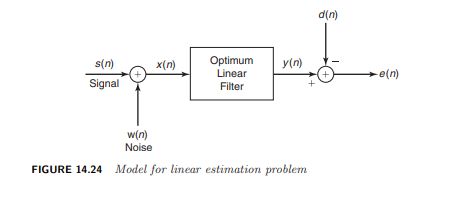
\includegraphics[width=1\linewidth]{LinearEstimationModel.png}
\end{figure}
In this section, we treat the problem of signal estimation in the
presence of an additive noise disturbance. The estimator is constrained
to be a linear filter with impulse response h(n), which is designed so
that its output approximates some specified desired signal process D(n),
with sample sequence d(n). Figure 14.24 illustrates the linear estimation
problem.
The filter's input sequence is x(n) = s(n) + w(n) and its output
sequence is y(n)—that is, a sample sequence of the process Y(n). The
difference between the desired signal and the filter output is the error
sequence e(n) = d(n) - y(n), with the underlying process denoted by
E(n). We distinguish three special cases: \\
\vspace{1em}
(a) If d(n) = s(n), the linear estimation problem is referred to as filtering. \\
\vspace{1em}
(b) If $d(n) = s(n + D)$, where $D > 0$, the linear estimation problem is 
referred to as signal prediction. Note that this problem is different
than the prediction considered in the previous section, where d(n) =
x(n + D), D $\geq$ 0. \\
\vspace{1em}
(c) If d(n) = s(n - D), where $D > 0$, the linear estimation problem is
termed signal smoothing. \\
\vspace{1em}
The basic assumptions
are that the processes S(n), W(n), and D(n) are zero mean and wide-sense
stationary. The linear filter will be assumed to be either FIR or IIR. If it is
IIR, we assume that the input data x(n) is available over the infinite past.
We begin with the design of the optimum FIR filter. The optimum linear
filter, in the sense of minimum mean-square error (MMSE), is called a
Wiener filter.

\subsubsection{FIR Wiener Filter}
Suppose that the filter is constrained to be of length M with coefficients
h(k), $0 \leq k \leq M-1$. Hence its output y(n) depends on the finite data
record $x(n), x(n-1),...,x(n-M+1),$
\begin{equation}
y(n) = \sum_{k=0}^{M-1}h(k)x(n-k)
\end{equation}
The mean-square value of the error between the desired output d(n) and
the actual output y(n) is
\[
\mathrm{E} \left[ \left( D(n) - \sum_{k=0}^{M-1} h(k) X(n-k) \right)^2 \right]
\]
The equation for the Wiener prediction filter :
\begin{equation}
\sum_{k=0}^{M-1}h(k)[R_{ss}(l-k)+R_{WW}(l-k)]=R_{SS}(\ell+D), \space \ell = 0,1,...M-1
\end{equation}\
Let us consider a signal x(n) = s(n) + w(n), where s(n) is a sample sequence
of an AR(1) process S(n) that satisfies the difference equation
\begin{center}
$s(n) = 0.6s(n-1)+v(n)$
\end{center}
where v(n) is a sample sequence of a white noise process V(n) with variance $\sigma_V^2=0.64$ and w(n) is a sample sequence of a white noise process W(n) with variance $\sigma^2_W=1$. \\
\vspace{1em}
a. Design a Wiener FIR filter of length M = 2 to estimate the desired signal
S(n). \\
b. Use MATLAB to design the optimum FIR Wiener filter for lengths M = 3, 4,
and 5, and the corresponding MMSE for these cases. Comment on how the
MMSE changes as M is increased from M = 2 to M = 5. \\
\vspace{1em}
Since S(n) is obtained by exciting a single-pole filter by white noise, the power
spectral density of S(n) is 
\begin{center}
$S_{SS}(f) = \sigma_V^2|H(e^{j2\pi f})|^2=\frac{0.64}{|1-0.6e^{-j2\pi f}|^2}=\frac{0.64}{1.36-1.2\cos(2\pi f)}$
\end{center}
Using the procedure given in Example 13.14, the corresponding autocorrelation
sequence $R_{SS}(m)$ is
\begin{center}
$R_{SS}(m)=(0.6)^{|m|}$
\end{center}
a. The equations for the filter coefficients are
\begin{center}
2h(0) + 0.6h(1) = 1 \\
\vspace{1em}

0.6h(0) = 2h(1) = 0.6  \\
\vspace{1em}
Solutions of these equations yields the result \\
\vspace{1em}
h(0) = 0.451,  \space \space h(1) = 0.165 \\
\vspace{1em}
The corresponding minimum MSE is \\
\vspace{1em}
MMS$E_2$ = $1-h(0)R_{SS}(0)-h(1)R_{SS}(1) = 1 - 0.451 -(0.165)(0.6) = 0.45$
\end{center}
\begin{lstlisting}
 varW = 1; M = 2; m = 0:M-1;
 Rss = 0.6.^m; TM = toeplitz(Rss) + varW*eye(M);
 RD = Rss';
 hopt2 = TM\RD
hopt2 =
0.4505
0.1648
 MMSE2 = Rss(1) - RD'*hopt2
MMSE2 =
0.4505
\end{lstlisting}
The filter coefficients and the corresponding MMSE values are obtained
using the following MATLAB script.
\begin{lstlisting}
 M = 3; m = 0:M-1;
 Rss = 0.6.^m; TM = toeplitz(Rss) + varW*eye(M); RD = Rss';
 hopt3 = TM\RD; MMSE3 = Rss(1) - RD'*hopt3
MMSE3 =
0.4451
 M = 4; m = 0:M-1;
 Rss = 0.6.^m; TM = toeplitz(Rss) + varW*eye(M); RD = Rss';
 hopt4 = TM\RD; MMSE4 = Rss(1) - RD'*hopt4
MMSE4 =
0.4445
 M = 5; m = 0:M-1;
 Rss = 0.6.^m; TM = toeplitz(Rss) + varW*eye(M); RD = Rss';
 hopt5 = TM\RD; MMSE5 = Rss(1) - RD'*hopt5
MMSE5 =
0.4445
 MMSE = [MMSE2,MMSE3,MMSE4,MMSE5];
 % Plotting commands follow
\end{lstlisting}
 \begin{figure}[H]
     \centering
     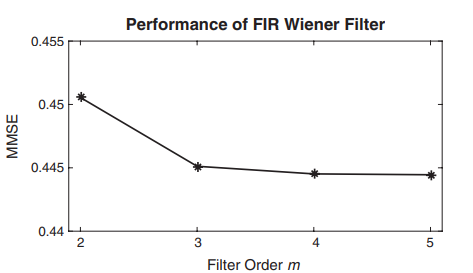
\includegraphics[width=1\linewidth]{FIRWienerPerformance1.png}
     \caption{Plot of MMSE vs. filter order }
 \end{figure}
a. Repeat the above example when the variance of V(n) = $\sigma^2_V=0.64$ and the
variance of the additive noise W(n) is $\sigma^2_W = 0.1$ \\
b. Generate the AR(1) signal sequence s(n) and the corresponding received
sequence
\begin{center}
x(n) = s(n) + w(n), $0 \leq n \leq 1000$ \\
\vspace{1em}

Filter the sequence x(n), $0 \leq n \leq 1000$, by the Wiener filter with M =
2, 3, 4, 5 and plot the output $y_2(n), y_3(n), y_4(n)$, and $y_5(n)$, along with the
derived signal s(n). Comment on the effectiveness of the Wiener filter in
estimating the derived signal s(n).
\end{center}
The PSD and autocorrelation of S(n), respectively, are
given by
\begin{center}
    $S_{SS}(f) = \frac{0.64}{1.36-1.2\cos2\pi f}$ \\
    $R_{SS}(m)=0.64^{|m|}$
\end{center}
\begin{lstlisting}
 varW = 0.1; M = 2; m = 0:M-1;
 Rss = 0.6.^m; TM = toeplitz(Rss) + varW*eye(M);
 RD = Rss';
 hopt2 = TM\RD;
 MMSE2 = Rss(1) - RD'*hopt2
MMSE2 =
0.0871
 M = 3; m = 0:M-1;
 Rss = 0.6.^m; TM = toeplitz(Rss) + varW*eye(M); RD = Rss';
 hopt3 = TM\RD; MMSE3 = Rss(1) - RD'*hopt3
MMSE3 =
0.0870
 M = 4; m = 0:M-1;
 Rss = 0.6.^m; TM = toeplitz(Rss) + varW*eye(M); RD = Rss';
 hopt4 = TM\RD; MMSE4 = Rss(1) - RD'*hopt4
MMSE4 =
0.0870
 M = 5; m = 0:M-1;
 Rss = 0.6.^m; TM = toeplitz(Rss) + varW*eye(M); RD = Rss';
 hopt5 = TM\RD; MMSE5 = Rss(1) - RD'*hopt5
MMSE5 =
0.0870
 % Plotting commands follow    
\end{lstlisting}
Clearly, the MMSE values are very small and quickly settle into a
steady-state value of 0.0807.
\begin{figure}[H]
    \centering
    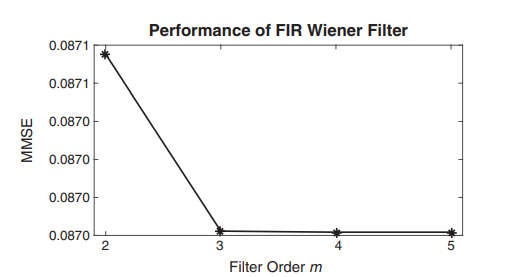
\includegraphics[width=1\linewidth]{MMSE2.png}
\end{figure}
Signal generation and Wiener filtering operations are given in the following
MATLAB script.
\begin{lstlisting}
 n = 0:1000; varW = 0.1;
 varV = 0.64; vn = sqrt(varV)*randn(1,length(n));
 sn = filter(1,[1-0.6],vn);
 wn = sqrt(varW)*randn(1,length(n));
 xn = sn + wn;
 yn2 = filter(hopt2,1,xn);
 yn3 = filter(hopt3,1,xn);
 yn4 = filter(hopt4,1,xn);
 yn5 = filter(hopt5,1,xn);    
\end{lstlisting}
\begin{figure}[H]
    \centering
    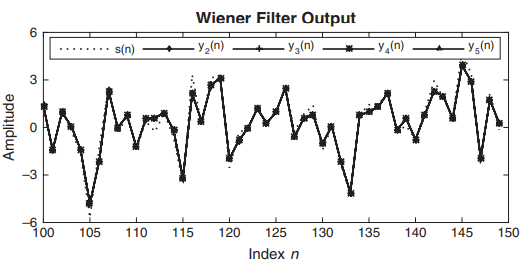
\includegraphics[width=1\linewidth]{WienerFilterResponse.png}
    \caption{Plots of signal s(n) and Wiener filter estimates $y_k(n)|_{k=2}^{5}$}
\end{figure}






































































\newpage
\section{Applications of Adaptive Filtering (unfinished)}
In contrast to the filter design techniques considered in those two
chapters, there are many digital signal processing applications in which
the filter coefficients cannot be specified a priori. For example, let us consider a high-speed modem that is designed to transmit data over telephone
channels. Such a modem employs a filter called a channel equalizer to compensate for the channel distortion. The modem must effectively transmit
data through communication channels that have different frequency response characteristics and hence result in different distortion effects. The
only way in which this is possible is if the channel equalizer has adjustable
coefficients that can be optimized to minimize some measure of the distortion, on the basis of measurements performed on the characteristics of
the channel. Such a filter with adjustable parameters is called an adaptive
filter—in this case, an adaptive equalizer. Numerous applications of adaptive filters have been described in the
literature. Some of the more noteworthy applications include (1) adaptive
antenna systems, in which adaptive filters are used for beam steering and
for providing nulls in the beam pattern to remove undesired interference
[97], (2) digital communication receivers, in which adaptive filters are
used to provide equalization of intersymbol interference and for channel identification [81], (3) adaptive noise canceling techniques, in which an
adaptive filter is used to estimate and eliminate a noise component in
some desired signal [96, 34, 15], and (4) system modeling, in which an
adaptive filter is used as a model to estimate the characteristics of an unknown system. These are just a few of the best-known examples on the use
of adaptive filters.
Although both IIR and FIR filters have been considered for adaptive filtering, the FIR filter is by far the most practical and widely used.
The reason for this preference is quite simple. The FIR filter has only
adjustable zeros, and hence it is free of stability problems associated with
adaptive IIR filters that have adjustable poles as well as zeros. We should
not conclude, however, that adaptive FIR filters are always stable. On the
contrary, the stability of the filter depends critically on the algorithm for
adjusting its coefficients.
Of the various FIR filter structures that we may use, the direct form
and the lattice form are the ones often used in adaptive filtering applications. An important consideration in the use of an adaptive filter is the
criterion for optimizing the adjustable filter parameters. The criterion
must not only provide a meaningful measure of filter performance, but it
must also result in a practically realizable algorithm.
One criterion that provides a good measure of performance in adaptive filtering applications is the least-squares criterion, and its counterpart
in a statistical formulation of the problem, namely, the mean-square-error
(MSE) criterion. The least-squares (and MSE) criterion results in a quadratic performance index as a function of the filter coefficients, and hence
it possesses a single minimum. The resulting algorithms for adjusting the
coefficients of the filter are relatively easy to implement.
In this chapter, we describe a basic algorithm, called the least-meansquare (LMS) algorithm, to adaptively adjust the coefficients of an FIR
filter. The adaptive filter structure that will be implemented is the direct form FIR filter structure with adjustable coefficients h(0), h(1),...,h(N-1)
\begin{figure}[H]
    \centering
    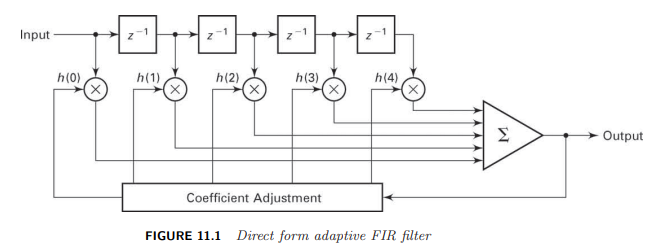
\includegraphics[width=1\linewidth]{AdaptiveFIR.png}
\end{figure}

\subsection{LMS algorithm for coefficient adjustment}
Suppose we have an FIR filter with adjustable coefficients $\{h(k), 0 \leq k \leq N - 1\}.$ Let \{x(n)\} denote the input sequence to the filter, and let the corresponding output be \{y(n)\} where 
\begin{equation}
y(n) = \sum_{k=0}^{N-1}h(k)x(n-k), \space n =0,....,M 
\end{equation}
Suppose that we also have a desired sequence {d(n)} with which we can
compare the FIR filter output. Then we can form the error sequence
\{e(n)\} by taking the difference between d(n) and y(n), that is,
\begin{equation}
e(n) = d(n) - y(n), \space n = 0,...,M
\end{equation}
The coefficients of the FIR filter will be selected to minimize the sum of
squared errors. Thus we have
\begin{equation}
\epsilon = \sum_{n=0}^{M}d^2(n)-2\sum_{k=0}^{N-1}h(k)r_{dx}(k)+\sum_{k=0}^{N-1}\sum_{l=0}^{N-1}h(k)h(l)r_{xx}(k-l)
\end{equation}
where 
\begin{equation}
r_{dx}(k)= \sum_{n=0}^{M}d(n)x(n-k), \space0 \leq k \leq N -1
\end{equation}
\begin{equation}
r_{xx}(k)= \sum_{n=0}^{M}x(n)x(n+k), \space0 \leq k \leq N -1
\end{equation}
We call {rdx(k)} the cross-correlation between the desired output
sequence {d(n)} and the input sequence {x(n)}, and {rxx(k)} is the
autocorrelation sequence of {x(n)}. The sum of squared errors $\epsilon$ is a quadratic function of the FIR filter
coefficients. Consequently, the minimization of $\epsilon$ with respect to the filter
coefficients {h(k)} results in a set of linear equations. Hence, 
\begin{equation}
\sum_{k=0}^{N-1}h(k)r_{xx}(k-m)=r_{dx}(m), \space 0 \leq m \leq N -1
\end{equation}
the filter coefficients are updated according to the equation
\begin{equation}
h_n(k)=h_{n-1}(k)+\Delta *e(n)*x(n-k), 0 \leq k \leq N -1, n = 0,1,... 
\end{equation}
where $\Delta$ is is called the step-size parameter, x(n - k) is the sample of the
input signal located at the kth tap of the filter at time n, and e(n)x (n - k)
is an approximation (estimate) of the negative of the gradient for the kth
filter coefficient. This is the LMS recursive algorithm for adjusting the
filter coefficients adaptively so as to minimize the sum of squared errors $\epsilon$.
The step-size parameter $\Delta$ controls the rate of convergence of the
algorithm to the optimum solution.


\subsection{Projects}
\subsubsection{System Identification}
In system identification or system modeling, we have an unknown system,
called a plant, that we wish to identify. The system is modeled by an FIR filter with adjustable coefficients. Both the plant and model are excited
by an input sequence x(n). If y(n) denotes the output of the plant and $\bar{y}(n)$ denotes the output of the model
\begin{figure}
    \centering
    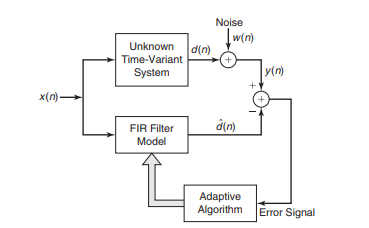
\includegraphics[width=1\linewidth]{SystemIdentification.png}
\end{figure}
\begin{equation}
\bar{y}(n) = \sum_{k=0}^{M-1}h(k)x(n-k)
\end{equation}
we may form the error sequence
\begin{equation}
e(n) = y(n) -\bar{y}(n), \space \space n = 0,1...
\end{equation}
and select the coefficients h(k) to minimize the sum of square errors, that is
\begin{equation}
\epsilon_M=\sum_{n=0}^{N}[y(n)-\sum_{n=0}^{M-1}h(k)x(n-k)]^2
\end{equation}
where N + 1 is the number of observations. This is the least-squares
criterion for determining the filter coefficients, which results in the set of
linear equations
\begin{equation}
\sum_{k=0}^{M-1}h(k)r_{xx}(l-k)=r_{yx}(l), \space \space l = 0, 1,...,M-1
\end{equation}
\begin{equation}
r_{xx}(l)=\sum_{n=0}^{N}x(n)x(n-l)
\end{equation}
\begin{equation}
r_{yx}(l)=\sum_{n=0}^{N}y(n)x(n-l)
\end{equation}
By solving (15.4), we obtain the filter coefficients for the model. Since
the filter parameters are obtained directly from measurement data at the
input and output of the system, without prior knowledge of the plant, we
call the FIR filter model an adaptive filter. If our only objective were to identify the system by use of the FIR
model, the solution of (15.4) would suffice. In control systems applications,
however, the system being modeled may be time-variant, changing slowly
with time, and our purpose for having a model is to ultimately use it for designing a controller that controls the plant. Furthermore, measurement
noise is usually present at the output of the plant. This noise introduces
uncertainty in the measurements and corrupts the estimates of the filter
coefficients in the model. Such a scenario is illustrated in Figure 15.2.
In this case, the adaptive filter must identify and track the time-variant
characteristics of the plant in the presence of measurement noise at the
output of the plant
\begin{center}
Consider the system identification problem as illustrated in the above figure. Suppose
the unknown system has two complex-conjugate poles with a system function
\begin{equation}
H(z) = \frac{1}{1-2Re(p)z^{-1}+|p|^2z^{-2}}
\end{equation}
\end{center}
where p is one of the poles. The additive noise sequence w(n) is a sample
sequence of a white, zero-mean Gaussian process W(n) with variance $\sigma^2_W=0.02$. The excitation sequence x(n) is also a sample sequence of a white, zero-mean Gaussian process X(n) with variance $\sigma^2_x=1$. The processes W(n) and X(n) are
uncorrelated (neither signal contains information about the other). The FIR filter model has impulse response h(n) for $0 \leq n \leq M - 1$ \\
\vspace{1em}
a. Generate the output sequence y(n) for $0 \leq n \leq 1000$ and the corresponding
desired sequence d(n) for $0 \leq n \leq 1000$, when p = $0.8e^{j\pi/4}$ andd M = 15. \\
\vspace{1em}
b. Compute the autocorrelation sequence $r_{xx}(m)$ and the cross-correlation sequence $r_{yx}(m) $ for $0 \leq m \leq M-1 $. Then compute the FIR filter coefficients
from the least-sequence equation. \\
\vspace{1em}
c. Plot and compare the impulse response of the unknown system with that of
the FIR filter model. Also plot and compare the frequency response of the
unknown system with that of the model. \\
\vspace{1em}
d. Repeat the parts (a), (b), and (c) when the sequence x(n) is the output of a
first-order AR process described by the difference equation
\begin{equation}
x(n) = \frac{1}{2}x(n-1)+v(n)
\end{equation}
where v(n) is a sample function of a white Gaussian noise process with
variance $\sigma^2_V=1$ \\
\vspace{1em}
a.
\begin{lstlisting}
 varW = 0.02; % Additive noise variance
 varX = 1; % Excitation seq Variance
 N = 1000; n = 0:N; % # of samples and indices
 p = 0.8*exp(1j*pi/4); % Pole location
 a = [1,-2*real(p),abs(p)^2]; % Plant denominator coeff
 M = 15; % FIR filter model order
 xn = sqrt(varX)*randn(N+1,1); % Input sequence
 wn = sqrt(varW)*randn(N+1,1); % Noise sequence
 dn = filter(1,a,xn); % Output of the plant
 yn = dn+wn; % Noisy plant output   
\end{lstlisting}
b. 
\begin{lstlisting}
 [rxx,lags] = xcorr(xn,M-1); % ACRS of x(n)
 Rxx = toeplitz(rxx(M:end)); % ACRM of x(n)
 ryx = xcorr(yn,xn,M-1); % CCRS between y(n) and x(n)
 ryx = ryx(M:end); % CCRV between y(n) and x(n)
 hm = Rxx\ryx; % Model coeff (or Imp resp)
 hp = impz(1,a,M+5); % Plant impulse response    
\end{lstlisting}
c.
\begin{lstlisting}
 om = linspace(0,1,1001)*pi;
 Hm = freqz(hm,1,om);
 Hm_mag = abs(Hm);
 Hm_pha = angle(Hm)/pi;
 Hp = freqz(1,a,om);
 Hp_mag = abs(Hp);
 Hp_pha = angle(Hp)/pi;
 % Plotting commands follow    
\end{lstlisting}
\begin{figure}[H]
    \centering
    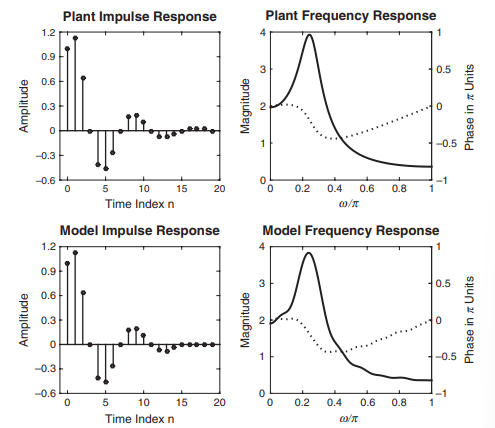
\includegraphics[width=1\linewidth]{PlantModel1.png}
\end{figure}
d.
\begin{lstlisting}
 varW = 0.02; % Additive noise variance
 varV = 1; % Excitation seq Variance
 N = 1000; n = 0:N; % Number of samples and indices
 p = 0.8*exp(1j*pi/4); % Pole location
 a = [1,-2*real(p),abs(p)^2]; % Plant denominator coeff
 M = 15; % FIR filter model order
 vn = sqrt(varV)*randn(N+1,1); % Gaussian seq for Input x(n)
 xn = filter(1,[1,-1/2],vn); % Input sequence x(n)
 wn = sqrt(varW)*randn(N+1,1); % Noise sequence
 dn = filter(1,a,xn); % Output of the plant
 yn = dn+wn; % Noisy plant output
 [rxx,lags] = xcorr(xn,M-1); % ACRS of x(n)    
 Rxx = toeplitz(rxx(M:end)); % ACRM of x(n)
 ryx = xcorr(yn,xn,M-1); % CCRS between y(n) and x(n)
 ryx = ryx(M:end); % CCRV
 hm = Rxx\ryx; % Model coeff (or Imp resp)
 hp = impz(1,a,M+5); % Plant impulse response
 om = linspace(0,1,1001)*pi;
 Hm = freqz(hm,1,om);
 Hm_mag = abs(Hm); Hm_pha = angle(Hm)/pi;
 Hp = freqz(1,a,om);
 Hp_mag = abs(Hp); Hp_pha = angle(Hp)/pi;
\end{lstlisting}
\begin{figure}[H]
    \centering
    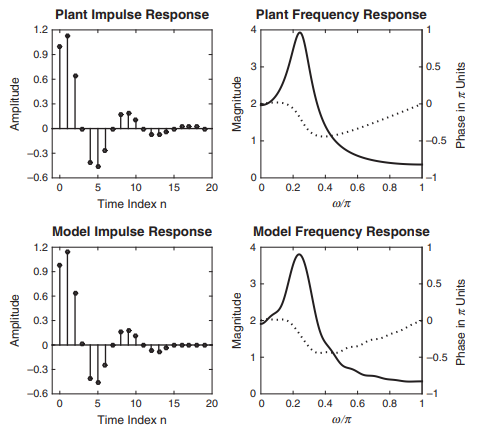
\includegraphics[width=1\linewidth]{PlantModel2.png}
\end{figure}
\newpage
\section{Terminology}
Synthesizer - A device used to produce oscillations (i.e. Oscilloscope) \\
\vspace{1em}
Quantizer - A device that is used for number arithmetic processing in A/D and D/A conversion (i.e. Raspberry Pi) \\
\vspace{1em}
Aliasing - Refers to distortion. Aliasing occurs when a signal's frequencies is greater than half the sampling rate (Nyquist rate). When a signal is an alias, it cannot appear unique to other signals, whereas signals less than half the sampling rate do appear unique. \\
\vspace{1em}
Round-off error - The rounding error associated with D/A and A/D conversion. Non floating point hardware generally have a lot of round-off errors. \\
\vspace{1em}
Equalizer - An equalizer (EQ) is a type of filter system used to adjust the balance of frequency components in a signal, most commonly audio. (literally makes the frequency response balanced, hende the term "equalizer") \\
\vspace{1em}
Autocorrelation - Measure of the how similar a signal is to itself after being shifted over and over. Used to check for periodicity. If it is non periodic, we generally consider the signal to be a random process (speech, noise, etc.). \\
\vspace{1em}
Band-limited - A signal is band-limited if there exists a finite radian frequency $\Omega_0$ such that $X_a(j\Omega)$ is zero for $|\Omega| > \Omega_0$. The frequency $F_0 = \Omega_0/2\pi$ is
called the signal bandwidth in Hz. \\
\vspace{1em}
Reconstruction - This is the reconstruction of a digital signal into an analog signal. \\
\vspace{1em}
MSE -  (Mean Square Error): The average squared difference between the estimated values and the true value \\
\vspace{1em}
Correlation - Signals are said to be correlated when one signal contains information about the other signal. This comes up in adaptive and wiener filtering \\
\vspace{1em}
Gortzeal Algorithm 




































\newpage
\section{GNU Octave} 
Solid alternative to MATLAB and completely free
\newpage

\section{Embedded Systems}
Embedded systems are absolutely needed for real time signal processing

\subsection{SPI vs $I^2C$}
\begin{tabular}{|c|c|c|}
\hline
\textbf{Term} & \textbf{SPI} & \textbf{$I^2C$}  \\
\hline
Simplicity & Simple protocol & More complex logic \\
\hline
Speed & Faster (1–50+ MHz) & Slower (100 kHz–3.4 MHz) \\
\hline
Wires & 4 (min) & 2 \\
\hline
Scalability & Needs extra CS pins & Supports many devices via addresses \\
\hline
Direction & Full-duplex & Half-Duplex\\
\hline
Noise immunity & Less (noisy at high speed) & Better (open-drain)\\
\hline
Throughput & High & Medium \\
\hline
Applications & High-speed DACs, audio, SD cards & Sensors, EEPROMs, slow peripherals \\
\hline
\end{tabular}
\section{SIMD Programming for ARM Cortex M4}
Capable of processing multiple data with a single instruction, SIMD operations are widely used for 3D graphics and audio/video processing in multimedia applications. 
\begin{figure}[H]
    \centering
    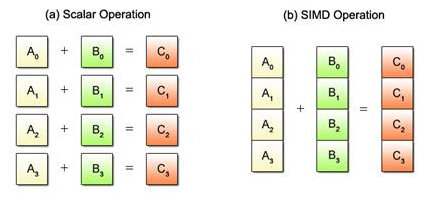
\includegraphics[width=1\linewidth]{SIMD_EX1.png}
\end{figure}
With conventional scalar operations, four add instructions must be executed one after another to obtain the sums as shown in Fig. 2.1 (a). Meanwhile, SIMD uses only one add instruction to achieve the same result, as shown in Fig. 2.1 (b). Requiring fewer instructions to process a given mass of data, SIMD operations yield higher efficiency than scalar operations.
\subsection{Restrictions}
Despite the advantage of being able to process multiple data per instruction, SIMD operations can only be applied to certain predefined processing patterns. Fig. 2.2 shows one such pattern where the same add operation is performed for all data.
\begin{figure}[H]
    \centering
    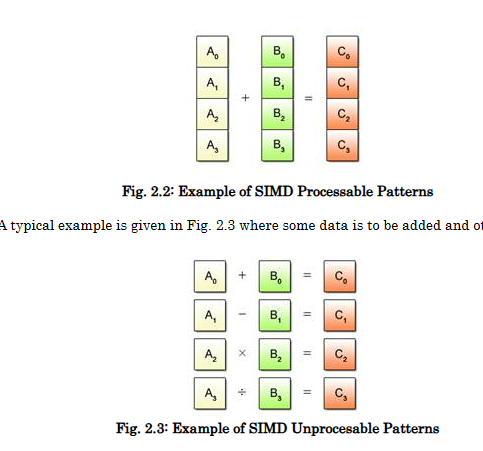
\includegraphics[width=1\linewidth]{SIMD_Restrictions.png}
\end{figure}
\subsection{Data used in SIMD Programming}
Conventional data types used in the C programming language, such as char, int and float, are called scalar types. Data types used for SIMD operations are called vector types. Each vector type has its corresponding scalar type as shown below \\
\begin{tabularx}{\textwidth}{|X|X|}
\hline
\textbf{Vector Type} & \textbf{Data} \\
\hline

\_\_vector unsigned char & 	
Sixteen unsigned 8-bit data \\
\hline
\_\_vector signed  char & 	
Sixteen signed 8-bit data \\ 
\hline
\_\_vector unsigned short & 	
Eight unsigned 16-bit data \\
\hline
\_\_vector signed short & 	
Eight signed 16-bit data \\
\hline
\_\_vector unsigned int & 	
Four unsigned 32-bit data \\
\hline
\_\_vector signed int & 	
Four signed 32-bit data \\
\hline
\_\_vector unsigned long long & 	
Two unsigned 64-bit data \\
\hline
\_\_vector signed long long & 	
Two signed 64-bit data \\
\hline
\_\_vector float & 	
Four single-precision floating-point data \\
\hline
\_\_vector double & 	
Two double-precision floating-point data \\
\hline
\end{tabularx}
The Cell uses 128-bit (16-byte) fixed-length vectors made up of 2 to 16 elements according to the data type. A vector can be interpreted as a series of scalars of the corresponding type (char, int, float and so on) in a 16-byte space. As shown in Fig. 2.4
\begin{figure}[H]
    \centering
    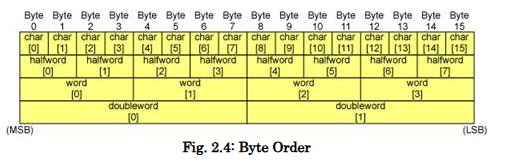
\includegraphics[width=1\linewidth]{ByteThing.png}
\end{figure}
\textbf{Vector Literal} is another data type. A vector literal is written as a parenthesized vector type followed by a curly braced set of constant expressions. The elements of the vector are initialized to the corresponding expression. Elements for which no expressions are specified default to 0. Vector literals may be used either in initialization statements or as constants in executable statements.
\begin{lstlisting}[language=C]
void func_a(void)
{
    __vector signed int va = (__vector signed int) { -2, -1,  1,  2 };    
\end{lstlisting}
\begin{lstlisting}[language=C]
va = vec_add(va, ((__vector signed int) { 1, 2, 3, 4 }));   
\end{lstlisting}
\begin{tabularx}{\textwidth}{|X|X|}
\hline
\textbf{Vector Type} & \textbf{Data} \\
\hline

(\_\_vector unsigned char)\{unsigned char,…\} & 	
Sixteen unsigned 8-bit data \\
\hline
(\_\_vector signed char)\{signed char,…\} & 	
Sixteen signed 8-bit data \\ 
\hline
(\_\_vector unsigned short)\{unsigned short,…\} & 	
Eight unsigned 16-bit data \\
\hline
(\_\_vector signed short)\{signed short,…\} & 	
Eight signed 16-bit data \\
\hline
(\_\_vector unsigned int)\{unsigned int,…\} & 	
Four unsigned 32-bit data \\
\hline
(\_\_vector signed int)\{signed int,…\} & 	
Four signed 32-bit data \\
\hline
(\_\_vector unsigned long long)\{unsigned long long,…\} & 	
Two unsigned 64-bit data \\
\hline
(\_\_vector signed long long)\{signed long long,…\} & 	
Two signed 64-bit data \\
\hline
(\_\_vector float)\{float,…\} & 	
Four single-precision floating-point data\{ unsigned int,…\} \\
\hline
(\_\_vector double)\{double,…\} & 	
Two double-precision floating-point data\{ unsigned int,…\} \\
\hline
\end{tabularx}
\subsection{Relationship between Vectors and Scalars}
With SIMD programming, there often arises a need to refer to a specific vector element as a scalar or to refer to a block of scalars as a single vector. This section describes the referencing method to meet that need, which, for example, makes it possible to output only the third element of a vector or to bundle scalar array input data into vectors suitable for SIMD processing.
\subsection{SIMD Operations}
This section describes SIMD operations using a summation as an example of simple arithmetic operations
\subsubsection{Addition}
Suppose that four add operations, each adding two numbers together, are required.
\begin{lstlisting}[language=C]
int a[4] = { 1, 3, 5, 7 };

int b[4] = { 2, 4, 6, 8 };

int c[4];


c[0] = a[0] + b[0];     // 1 + 2

c[1] = a[1] + b[1];     // 3 + 4
c[2] = a[2] + b[2];     // 5 + 6
c[3] = c[3] + c[3];     // 7 + 8
\end{lstlisting}
Scalar operations are based on a rule of “single data = single data + single data”. That is, the four add instructions in the example must be executed in sequence as stated in the 5th to 8th lines of the program in order to obtain the sums for all four equations. The SIMD equivalent program is written below 
\begin{lstlisting}[language=C]
 1 int a[4] __attribute__((aligned(16))) = { 1, 3, 5, 7 };

 2 int b[4] __attribute__((aligned(16))) = { 2, 4, 6, 8 };

 3 int c[4] __attribute__((aligned(16)));

 4

 5 __vector signed int *va = (__vector signed int *) a;

 6 __vector signed int *vb = (__vector signed int *) b;

 7 __vector signed int *vc = (__vector signed int *) c;

 8

 9 *vc = vec_add(*va, *vb);    // 1 + 2, 3 + 4, 5 + 6, 7 + 8    
\end{lstlisting}
SIMD operations process data on the principle of “multiple data = multiple data + multiple data”. This means that SIMD operations can process a greater quantity of data per instruction than scalar operations, making it possible to reduce the number of instructions necessary to be executed and thus the time required for processing.
\section{Arduino Uno R4}
The MCU for the Arduino Uno R4 is the RA4M1.

 
\subsection{Clocks}
The clock associated with the DAC12 is Peripheral module clock B (PCLKB). \\
The clock associated with ADC14 is Peripheral module clock C (PCLKC). \\
https://www.nongnu.org/avr-libc/user-manual/modules.html
\begin{figure}[H]
    \centering
    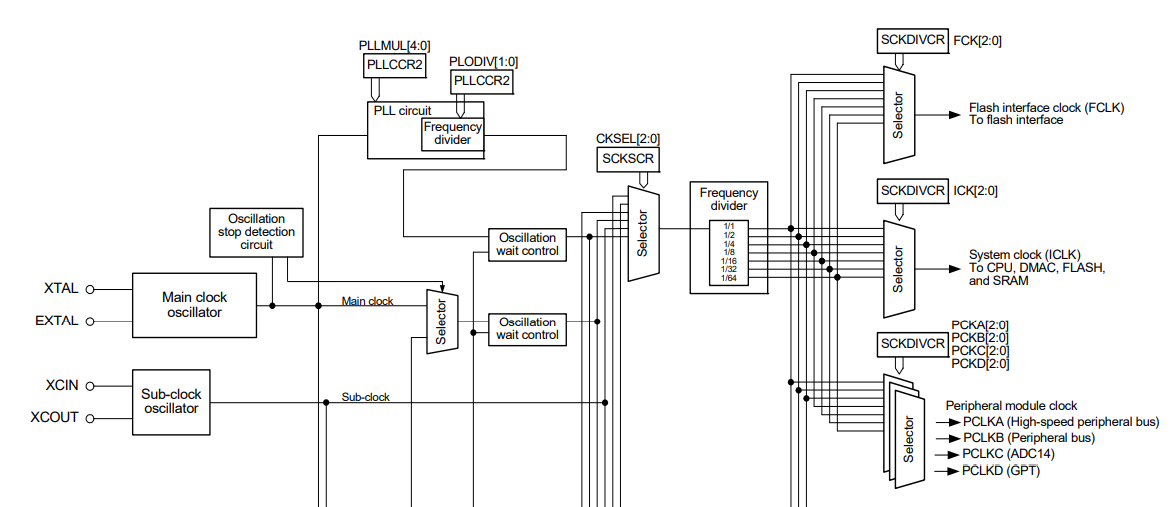
\includegraphics[width=1\linewidth]{ClockGenerationCircuit.png}
    \caption{Clock Generation Circuit}
\end{figure}
Both PCLKB and PCLKC can be found in the System Clock Division Control Register (SCKDIVCR). The address is SYSTEM.SCKDIVCR 4001 E020h. PCLKB is associated with b10 to b8 of this register. The clock can be prescaled by changing the bit values for b10 to b8, e.g. \\
\begin{center}
Bit prescaler setting for PCLKB \\
\vspace{1em}
\begin{tabular}{|c|c|c|c|}
    \hline
    b10 &  b9 & b8 & factor\\
     \hline
    0 &  0 & 0 & x1/1 \\
    \hline
    0 &  0 & 1 & x1/2 \\
    \hline
    0 &  1 & 0 & x1/4 \\
    \hline
    0 &  1 & 1 & x1/8 \\
    \hline
    1 &  0 & 0 & x1/16 \\
    \hline
    1 &  0 & 1 & x1/32 \\
    \hline
    1 &  1 & 0 & x1/64 \\
    \hline
\end{tabular}    
\end{center}
\begin{center}
PCLKC is one of the same \\
\vspace{1em}
\begin{tabular}{|c|c|c|c|}
    \hline
    b6 &  b5 & b4 & factor\\
     \hline
    0 &  0 & 0 & x1/1 \\
    \hline
    0 &  0 & 1 & x1/2 \\
    \hline
    0 &  1 & 0 & x1/4 \\
    \hline
    0 &  1 & 1 & x1/8 \\
    \hline
    1 &  0 & 0 & x1/16 \\
    \hline
    1 &  0 & 1 & x1/32 \\
    \hline
    1 &  1 & 0 & x1/64 \\
    \hline
\end{tabular}    
\end{center}
\subsection{Interrupts}
The Interrupt Controller Unit (ICU) controls which event signals are linked to the Nested Vector Interrupt Controller
(NVIC), Data Transfer Control (DTC), and Direct Memory Access Controller (DMAC) modules. The ICU also controls
non-maskable interrupts. Each peripheral can raise an interrupt request (IRQ), The NVIC can prioritize them (0–15 levels).
Will essentially allow for automatic sampling
\begin{figure}[H]
    \centering
    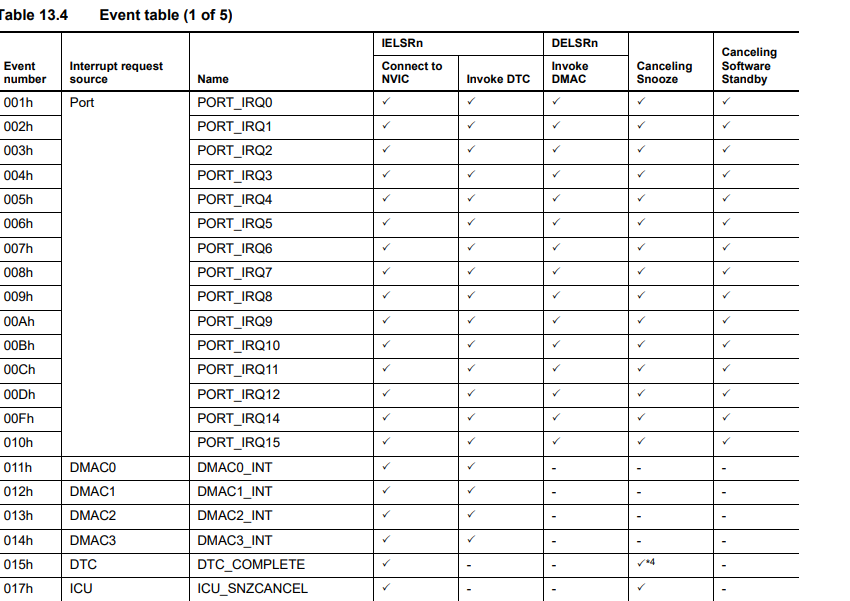
\includegraphics[width=1\linewidth]{EventTable1.png}
\end{figure}
\begin{figure}
    \centering
    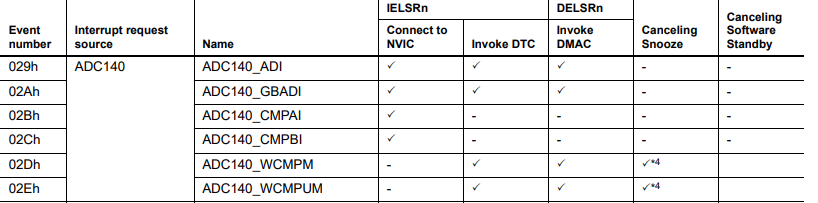
\includegraphics[width=1\linewidth]{EventTable2.png}
\end{figure}
\subsection{DMAC (unfinished)}
The MCU includes a 4-channel DMA Controller (DMAC) that can transfer data without intervention from the CPU.
When a DMA transfer request is generated, the DMAC transfers data stored at the transfer source address to the transfer
destination address.
\begin{figure}[H]
    \centering
    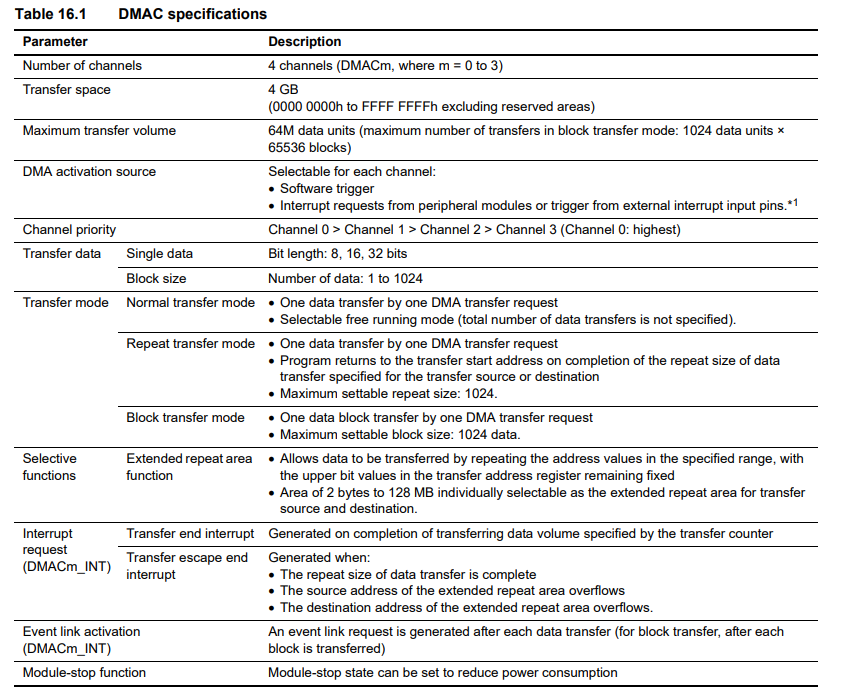
\includegraphics[width=1\linewidth]{DMAC1.png}
\end{figure}
\begin{figure}[H]
    \centering
    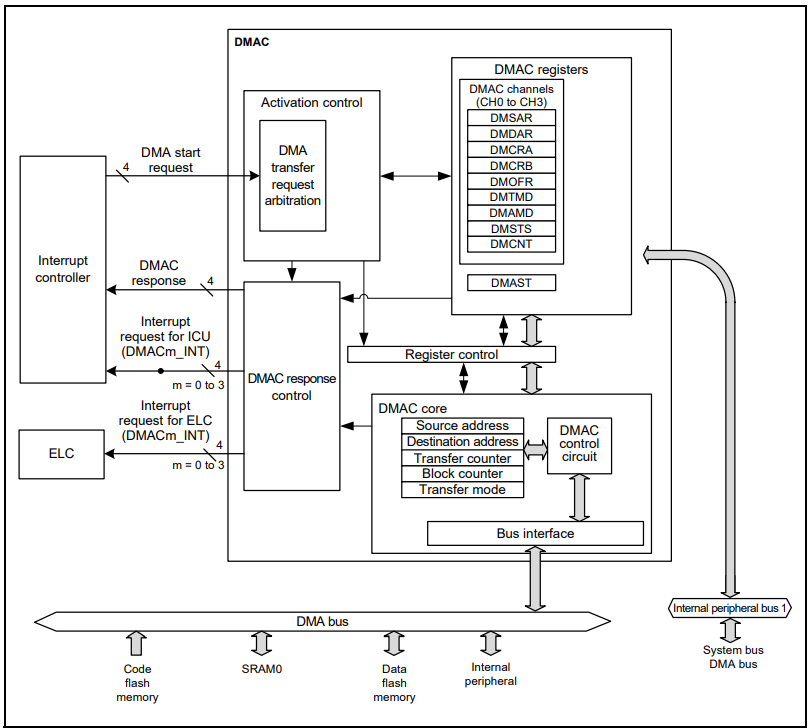
\includegraphics[width=1\linewidth]{DMAC2.png}
\end{figure}
\subsection{ELC (unfinished)}
\subsection{Asynchronous General-purpose Timer (AGT) (unfinished)}
\subsection{General PWM Timers (GPT32/GPT16) (unfinished)}
\subsection{SPI (unfinished)}
\subsection{DAC12 (unfinished)}
\begin{figure}[H]
    \centering
    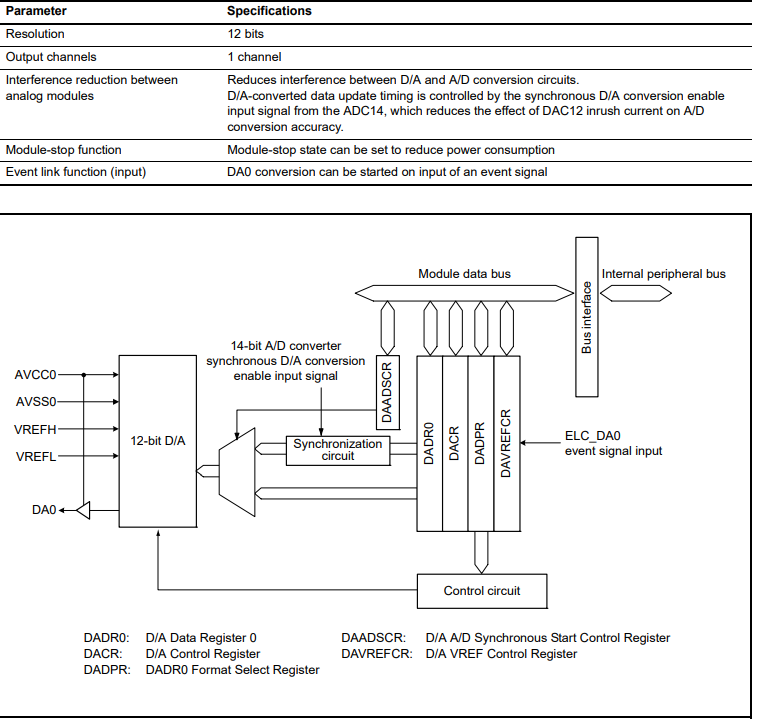
\includegraphics[width=1\linewidth]{DAC12BlockDiagram.png}
\end{figure}
\begin{figure}[H]
    \centering
    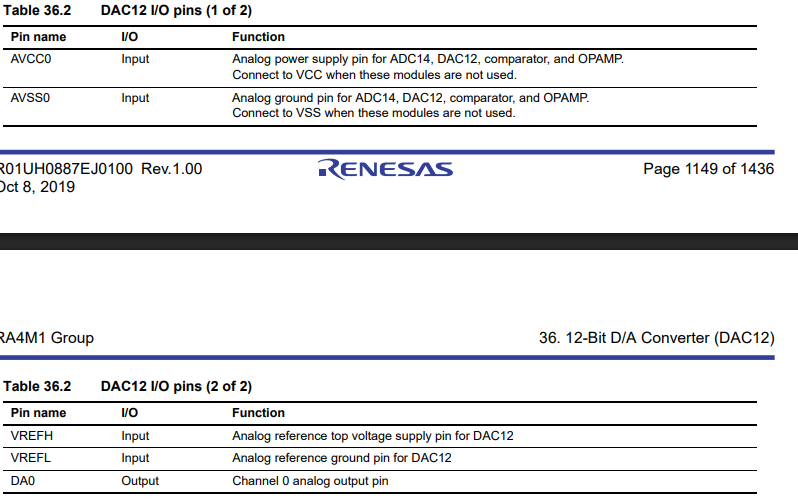
\includegraphics[width=1\linewidth]{DAC12IO.png}
\end{figure}
\subsection{ADC14 (unfinished)}
https://renesas.github.io/fsp/
\begin{figure}[H]
    \centering
    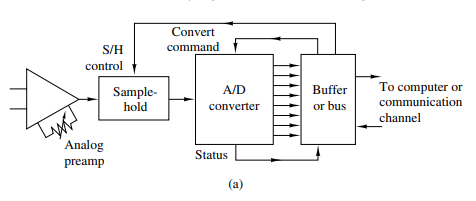
\includegraphics[width=1\linewidth]{ADBlockDiagram.png}
\end{figure}
\begin{figure}[H]
    \centering
    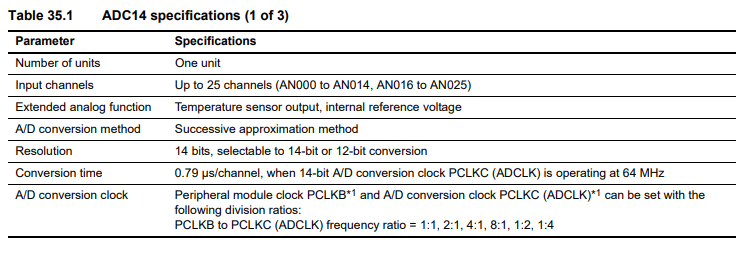
\includegraphics[width=1\linewidth]{ADC14Spec1.png}
\end{figure}
\begin{figure}[H]
    \centering
    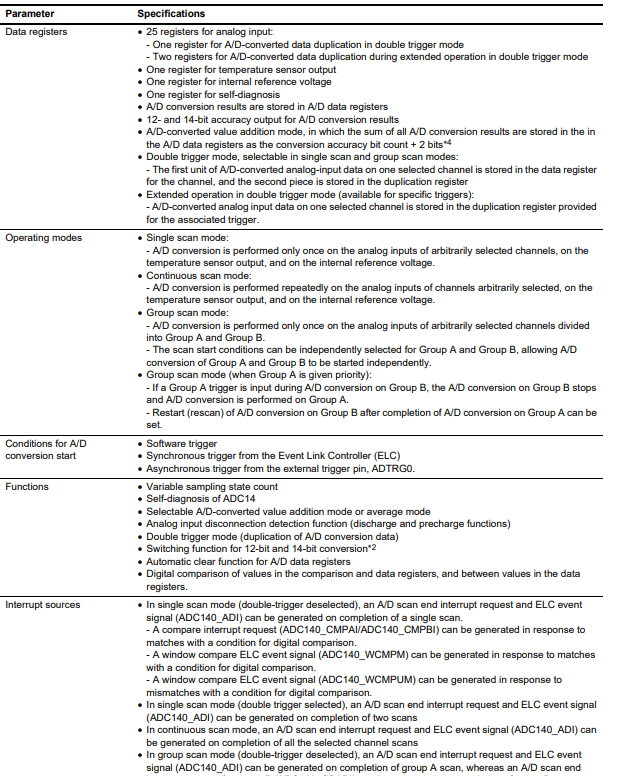
\includegraphics[width=1\linewidth]{ADC14Spec2.png}
\end{figure}
\begin{figure}[H]
    \centering
    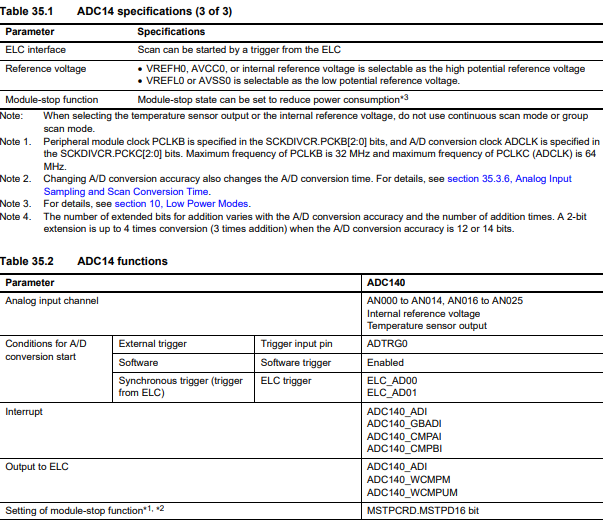
\includegraphics[width=1\linewidth]{ADC14Spec3.png}
\end{figure}
\begin{figure}[H]
    \centering
    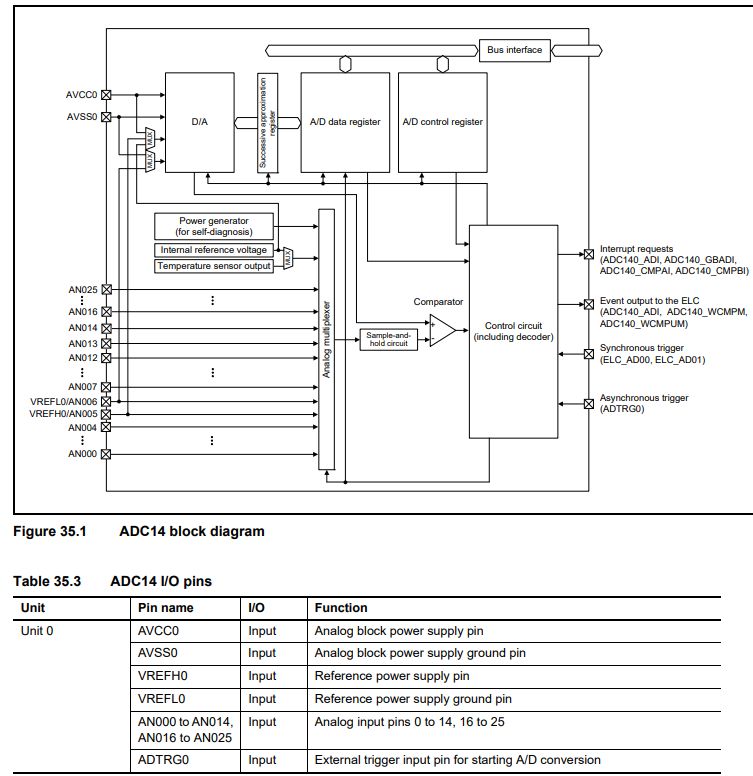
\includegraphics[width=1\linewidth]{BlockDiagramADC14.png}
\end{figure}
\newpage
















\section{Design Problems}
\subsection{A/D \& DAC }
\subsubsection{D/A on Raspberry Pi using FOH}
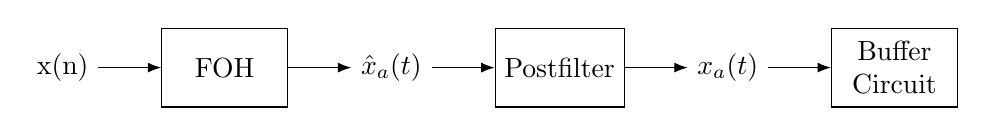
\begin{tikzpicture}[
  node distance=1.8cm and 0.8cm,
  box/.style={draw, minimum width=1.6cm, minimum height=1cm,align=center},
  arrow/.style={-Latex}
]
    

% Nodes
\node[] (n1) {x(n)};
\node[box, right=of n1] (n2) {FOH};
\node[right=of n2] (n3) {$\hat{x}_a(t)$};
\node[box, right=of n3] (n4) {Postfilter};
\node[right=of n4] (n5) {$x_a(t)$};
\node[box, right=of n5] (n6) {Buffer \\ Circuit};
% Pointers
\draw[arrow] (n1) -- (n2);
\draw[arrow] (n2) -- (n3);
\draw[arrow] (n3) -- (n4);
\draw[arrow] (n4) -- (n5);
\draw[arrow] (n5) -- (n6);
\end{tikzpicture} \\
\vspace{1em}
\begin{lstlisting}
mypi = raspi('192.168.0.16','thegotoman','tBh_4200');
configurePin(mypi,4,'DigitalOutput')

% First order hold
% Discrete - time signal x1(n) : Ts = 0.001
Ts = 0.001; n = -25:1:25; nTs = n* Ts ; x = exp ( -1000* abs ( nTs ));
%Plots
subplot (2 ,1 ,2) ; plot ( nTs *1000 , x);
xlabel ('t in msec '); ylabel ('Amplitude ')
title (' Reconstructed Signal from x_1 (n) Using FOH '); hold on
stem (n* Ts *1000 , x) ; hold off
% if Ts is 0.001 Fs = 1000 Hz so we must filter everything above the
% Nyquist rate 500 Hz 
while true
    for k=1:length(x)
        writeDigitalPin(mypi, 4, x(k) < 5); % Control the digital output based on x
        pause(Ts);
    end
end
\end{lstlisting}
Buffer Circuit:
\begin{figure}[H]
    \centering
    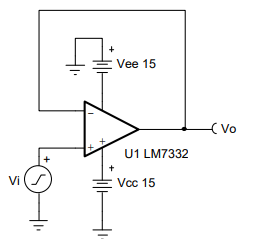
\includegraphics[width=0.25\linewidth]{Buffer.png}
\end{figure}
\subsection{IIR Filter Design}
\begin{lstlisting}
    
\end{lstlisting}

\section{Projects}
In Git: \\
cd: "$C:\backslash Users\backslash keeno\backslash OneDrive\backslash Documents\backslash MATLAB"$ \\
git init \\
git add Synthesizer\_App.mlapp \\
git commit -m "Initial commit"


\section{References}
\begin{enumerate}
  \setcounter{enumi}{0}  % Starts numbering from 2
  \item  V. K. Ingle and J. G. Proakis, \textit{Digital Signal Processing Using MATLAB V.4.} Brooks/Cole, 1997
  \item K. D. Rao and M. N. S. Swamy, \textit{Digital Signal Processing: Theory and Practice}. Singapore: Springer, 2018.
  \item D. G. Manolakis and V. K. Ingle, \textit{Applied Digital Signal Processing: Theory and Practice}. New York: Cambridge University Press, 2011.
  \item E. S. Gopi, \textit{Mathematical Summary for Digital Signal Processing Applications with Matlab}. Springer Science \& Business Media, 2010.
  \item T. B. Welch, Cameron H.G. Wright, and M. G. Morrow, \textit{Real-Time Digital Signal Processing from MATLAB® to C with the TMS320C6x DSPs, Second Edition}. CRC Press, 2011.
  \item R. Oshana, \textit{DSP software development techniques for embedded and real-time systems}. Burlington, Ma ; Oxford: Newnes, 2006.
  \item R. G. Lyons, \textit{Streamlining Digital Signal Processing}. John Wiley \& Sons, 2012.
  \item S. M. Kuo, B. H. Lee, and W. Tian, \textit{Real-Time Digital Signal Processing}. John Wiley \& Sons, 2006.
  \item N. Dahnoun, \textit{Multicore DSP}. Newark: John Wiley \& Sons, Incorporated, 2017
\end{enumerate}


\end{document}



